\documentclass[12pt,a4paper,oneside]{abntex2}
\usepackage[utf8]{inputenc}
\usepackage{amsmath}
\usepackage{esint}
\usepackage{amsfonts}
\usepackage{amssymb}
\usepackage{graphicx}
\usepackage{subfig}
\graphicspath{{fig/}}
\providecommand{\norm}[1]{\lVert#1\rVert}
\usepackage{empheq}
\usepackage{lscape}

%\usepackage[alf ,abnt-etal-cite=2 , abnt-year-extra-label=yes , abnt-etal-list=0, abnt-etal-text=it]{abntex2cite}

%capa
\autor{DAVID DA COSTA DE PINHO}% introduz nome do autor
\titulo{MODELAGEM MATEM\'ATICA E NUM\'ERICA DO EFEITO MAGNETO-EL\'ASTICO}
\data{2020}
\local{MACA\'E}

%anverso da folha de rosto
\preambulo{Tese apresentada ao Centro de Ci\^encia e Tecnologia da Universidade Estadual do Norte Fluminense, como parte das exig\^encias para conclus\~ao do curso de Doutorado.}
\orientador{Viatcheslav Ivanovich Priimenko, Ph.D}
\coorientador{Marcia Miranda Azeredo, D.Sc}
\tipotrabalho{monografia}

\begin{document}

\imprimircapa

\imprimirfolhaderosto%anverso

%{\ABNTEXchapterfont\Large\textsc{\imprimirautor}} - para aumentar a fonte e colocar em caixa alta

%importante dar enter para pular linha entre os tipos de textos

\begin{folhadeaprovacao}

\begin{center}
{\ABNTEXchapterfont\Large\bfseries\imprimirtitulo}\\\vspace{1cm}
{\ABNTEXchapterfont\Large\textsc{\imprimirautor}}
\end{center}

\vspace{1cm}
\hspace{.45\textwidth} \begin{minipage}{.5\textwidth}
\imprimirpreambulo
\end{minipage}

\vspace{1cm}
Trabalho aprovado em $\,19\,$ de Agosto de \imprimirdata.\\

\vspace{1cm}
Comiss\~ao Examinadora:\\
\assinatura{Prof. S\'ergio Gon\c{c}alves Pereira, D.Sc \\ FeMASS}
\assinatura{Prof. André Duarte Bueno, D.Sc \\ UENF}
\assinatura{Prof. Fernando Diogo de Siqueira, D.Sc \\ UENF}
\assinatura{Prof. Marcia Miranda Azeredo, D.Sc \\ UENF}
\assinatura{Prof Viatcheslav Ivanovich Priimenko, Ph.D\\ UENF}
%\assinatura{Prof. \imprimirorientador\\ UENF}

\begin{center}
\vfill
{\large\imprimirlocal}
\par
{\large\imprimirdata}
\end{center}

\end{folhadeaprovacao}

\begin{center}
{\ABNTEXchapterfont\Large\imprimirtitulo}\\\vspace{1cm}

\end{center}

\begin{resumo}
O objetivo principal desta obra \'e apresentar os fundamentos das teorias f\'isicas e matem\'atica relacionados ao efeito magneto-el\'astico, bem como um recondicionamento do modelo usado para descrever tal efeito. Inicialmente, apresentamos uma revis\~ao dos principais fen\^omenos pesquisados atualmente, envolvendo propaga\c{c}\~ao de ondas el\'asticas e eletromagn\'eticas. A mec\^anica do cont\'inuo e o eletromagnetismo s\~ao as duas teorias f\'isicas que descrevem a magneto-elasticidade, e introduzimos os principais conceitos dessas \'areas necess\'arios aos propositos desta monografia. Estudamos como ocorre o acoplamento entre ondas el\'asticas e eletromagn\'eticas bem como sua propaga\c{c}\~ao na subsuperf\'icie terrestre, atrav\'es de camadas estratigr\'aficas. Finalizamos com uma reescrita do modelo desse acoplamento de forma que possamos desenvolv\^e-lo analiticamente e produzir uma solu\c{c}\~ao num\'erica em trabalhos posteriores.
\\
Esta monografia tem por finalidade essencial o desenvolvimento anal\'itico do m\'etodo matricial de Ursin aplicado ao efeito magneto-el\'astico. Primeiramente, apresentamos uma revis\~ao sobre a utiliza\c{c}\~ao do m\'etodo matricial em problemas de prospec\c{c}\~ao de petr\'oleo, onde v\'arias dessas publica\c{c}\~oes foram produzidas no LENEP. Inclu\'imos uma sumariza\c{c}\~ao das ferramentas da f\'isica-matem\'atica necess\'arias ao entendimento desta obra. Transformamos as EDP's do efeito magneto-el\'astico em EDO's e mostramos como o m\'etodo matricial \'e utilizado na solu\c{c}\~ao de sistemas de EDO's que modelam a propaga\c{c}\~ao de ondas na subsuperf\'icie terrestre. Por fim, aplicamos o m\'etodo matricial nas EDO's da magneto-elasticidade de forma que possamos produzir um algoritmo computacional para obter as solu\c{c}\~oes numericamente.


\vspace{\onelineskip} 
\noindent 
\textbf{Palavras-chave}: Magneto-Elasticidade, Mec\^anica do Cont\'inuo, Equa\c{c}\~oes de Maxwell, Magneto-Elasticidade, M\'etodo Matricial de Ursin, Prospec\c{c}\~ao de Petr\'oleo.
\end{resumo}

\begin{center}
{\ABNTEXchapterfont\Large FOUNDATIONS OF MAGNETO-ELASTICITY}\\\vspace{1cm}
\end{center}

\begin{resumo}[Abstract]
\begin{otherlanguage*}{english}
The main purpose of this paper is present the foundations of physical and mathematical theories about magneto-elastic effect, and a reconditioning model to describe such effect. Firstly, we present a review of some phenomena found in current surveys, involving the propagations of elastic and eletromagnetics waves. Continuous mechanics and eletromagnetism describe magneto-elasticity, and we introduce a lots of required concepts from these areas to achieve the monography's goals. We also study how occurs the coupled propagation of elastic and eletromagnetics waves in Earth's subsurface, through stratigraphics layers. We finished rewriting the coupling's model in such manner that allow us to develope it analiticaly and to build a numerical solver in further works.
\\
This paper aims analitical development of Ursin's matricial method applied to magneto-elastic effect. First, we present a review about matricial method applied to different kind of oil prospecting issues, found in surveys produced in LENEP. Summaries of physical and mathematical tools required to understand this text were included. We transform magneto-elastic effect's PDE to ODE ones and we show how the matricial method can be usefull to solve ODE systems that describe propagations of waves in Earth's subsurface. Best for the last, we applied matricial method to magneto-elasticity's ODE in such way that we can build an algorithm to return numerical solutions.

\vspace{\onelineskip} 
\noindent 
\textbf{Keywords}: Magneto-Elasticity, Continuous Mechanics, Maxwell's Equations, Magneto-Elasticity, Ursin's Matricial Method, Oil Prospecting.

\end{otherlanguage*}
\end{resumo}

\listoffigures

\newpage

\tableofcontents

\textual

%\chapter{Introdução}
Esta monografia tem como finalidade principal o detalhamento da teoria que envolve o acoplamento de ondas eletromagnéticas e ondas elásticas que se propagam em meios estratificados, e homogêneos por camada, no subsolo terrstre. O desenvolvimento dessa teoria segue o modelo apresentado por \cite{erigen_1963} que trata da propagação de ondas elásticas num campo eletromagnético (geomagnético), onde essa propagação gera pequenas alterações geomagnéticas que se propagam, não com a velocidade da luz, mas ''acompanhando`` a onda elástica mantendo a velocidade desta última. 

A teoria é essencialmente uma combinação de eleasticidade infinitesimal e teoria eletromagnética linearizada, e para torna o texto o mais auto-didata possível, serão apresentados nos capítulos \ref{sec.fund_eletr} e \ref{sec.fund_elast} os principais conceitos e definições acerca das teorias básicas sobre eletromagnetismo e elasticidade. 

Esta monografia faz parte de um conjunto de pesquisas que objetivam desenvolver um novo modelo matemático-computacional para descrever os fenômenos que envolvem a propagação simultânea de ondas eletromagnéticas e elásticas em subsuperfície, de modo que tal levantamento possa ser usado para aprimorar as técnicas de exploração de petróleo ou outro bem mineiral.
%\chapter{Revis\~ao Bibliogr\'afica}

Existem diferentes tipos de modelos f\'isicos que descrevem as propaga\c{c}\~oes de ondas el\'asticas e eletromagn\'eticas bem como a intera\c{c}\~oes entre elas na subsuperf\'icie terrestre. A esses modelos s\~ao aplicados variados m\'etodos matem\'aticos e num\'ericos, incluindo o m\'etodo matricial, que realizam a simula\c{c}\~ao desses fen\^omenos f\'isicos. Apresentaremos nesse cap\'itulo algumas publica\c{c}\~oes nesse sentido, as quais est\~ao de alguma forma relacionadas ao objetivo desta monografia. 

\section{Prospec\c{c}\~ao Eletro-s\'ismica}

Alguns pesquisadores j\'a trabalharam em sistema acoplados, como \cite{White_Zhou_2006}, que estudaram fen\^omenos de \textit{Eletro-s\'ismica} que descrevem a convers\~ao de ondas eletromagn\'eticas em ondas s\'ismicas na subsuperf\'icie terrestre na prospec\c{c}\~ao de hidrocarbonetos. A convers\~ao entre as ondas ocorre em meios porosos onde uma onda eletromagn\'etica pode excitar uma onda s\'ismica de mesma frequ\^encia e vice-versa, atrav\'es do movimento dos fluidos contidos nos poros. A altera\c{c}\~ao que uma onda eletromagn\'etica promove numa onda s\'ismica de mesma frequ\^encia pode ser registrada na superf\'icie terrestre trazendo informa\c{c}\~oes sobre as propriedades el\'etricas da subsuperf\'icie. 


Esses estudiosos aplicam transformadas nas EDP's deduzidas por \cite{pride_94}, as quais passam a ser escritas como sistemas de EDO's. Utilizam o m\'etodo matricial contido em \cite{Ursin-1983} nessas EDO's para obter as solu\c{c}\~oes em cada camada estratigr\'afica e, por \'ultimo, retornam as solu\c{c}\~oes para o espa\c{c}o original. Ap\'os deduzir f\'ormulas explicitas, apresentam um algoritmo computacional onde os resultados num\'ericos s\~ao obtidos. Esse algoritmo pode ser modificado para computar separadamente a propaga\c{c}\~ao de ondas el\'asticas, ondas eletromagn\'eticas e as ondas da teoria de Biot. Como o artigo trata da produ\c{c}\~ao de onda s\'ismica atrav\'es de fontes eletromagn\'eticas, \'e necess\'ario um n\'ivel suficiente de corrente el\'etrica para que se produza uma resposta s\'ismica satisfat\'oria. 


Na figura \ref{fig.white_zhou} podemos observar um tra\c{c}o s\'ismico de fonte eletromagn\'etica obitdo pelo simulador, que \'e an\'alogo a um tra\c{c}o s\'ismico convencional. Note pela escala da figura que sinais muito pequenos podem ser identificados. Esses pequenos sinais t\^em no m\'aximo a amplitude dos ru\'idos provocados pela sensibilidade dos geofones e s\~ao menores do que muitas fontes de ru\'idos que podem ser identificadas no campos, da\'i uma m\'edia consider\'avel de sinais se faz necess\'aria para que a detec\c{c}\~ao seja plenamente confi\'avel. Como as equa\c{c}\~oes que descrevem os fen\^omenos s\~ao linearizadas, as escalas dos resultados tamb\'em s\~ao lineares com as correntes el\'etricas usadas como fonte, ent\~ao as pequenas respostas podem ser melhoradas com o aumento da corrente.
\begin{figure}
\centering
\includegraphics[scale=1]{white_zhou}
\caption{\textit{Tra\c{c}o s\'ismico obtido a partir de for\c{c}as eletromagn\'eticas como fonte.}}
\label{fig.white_zhou}
\end{figure}  

\section{M\'etodo Matricial em Meios Poroel\'asticos}\label{sec.matricial_poroelast}


\subsection{Sistema de Biot para Baixas Frequ\^encias}\label{sec.biot}

Alguns pesquisadores utilizaram o m\'etodo matricial em meios poroel\'asticos. Por exemplo,
\cite{Azeredo_2013} aplica o m\'etodo matricial para resolver de forma anal\'itico-num\'erica equa\c{c}\~oes de poroelasticidade deduzidas por Maurice Biot em 1956, as quais descrevem a propaga\c{c}\~ao de ondas em meio plano estratificado formado por camadas homog\^eneas e isotr\'opicas. 


Este trabalho apresenta dois tipos de fontes para produ\c{c}\~ao de ondas s\'ismicas:  uma fonte constitu\'ida por dinamite e uma fonte que emite uma for\c{c}a pontual vertical, que pode ser tipo martelo, queda de peso ou \textit{vibroseis}. O m\'etodo fornece f\'ormulas expl\'icitas para a constru\c{c}\~ao de algoritmo computacional  para obter a solu\c{c}\~ao do problema considerando que o fluxo de fluido \'e do tipo \textit{Poiseuille}, isto \'e, baixo n\'umero de \textit{Reynolds} e baixas frequ\^encias.

S\~ao apresentados alguns modelos geol\'ogicos para realiza\c{c}\~ao das simula\c{c}\~oes num\'ericas e cada modelo \'e testado utilizando diferentes frequ\^encias. Um desses modelos apresenta duas camadas horizontais homog\^eneas e isotr\'opicas com a interface terra-ar localizada em $z_0=0\,m$  e a superf\'icie de descontinuidade \'e dada na profundidade $z_1=1500\,m$. Al\'em disso,
considera-se que a camada 2 tem espessura infinita e a frequ\^encia de propaga\c{c}\~ao das ondas \'e de $15\,Hz$. Podemos visualizar na figura \ref{fig.marcia} o surgimento de dois eventos: o evento 1 representa a onda direta, a qual atinge o receptor sem que haja reflex\~ao em qualquer interface, e o segundo evento \'e a onda refletida na interface de descontinuidade entre a primeira e segunda camadas. S\~ao apresentados dois gr\'aficos simulando diferentes dist\^ancias entre fonte e receptor, pois assim \'e poss\'ivel analisar sua influ\^encia na amplitude do sinal registrado.
\begin{figure}
\centering
\includegraphics[scale=.77]{simograma_marcia}
\caption{\textit{Componente vertical da velocidade da matriz porosa. Frequ\^encia dominante da fonte igual a $15\,Hz$ e dist\^ancia fonte-receptor igual a: (a) $500\,m$ e (b) $1000\,m$.}}
\label{fig.marcia}
\end{figure}


Sendo assim, observa-se que, \`a medida em que a dist\^ancia fonte-receptor aumenta, passando de $500\,m$ para $1000\,m$, a amplitude do sinal registrado diminui. Isto acontece porque a amplitude da onda s\'ismica diminui com o passar do tempo devido \`a redistribui\c{c}\~ao da energia entre as fases durante da passagem da onda s\'ismica atrav\'es de meio poroso. 
%Observe que, como esse modelo \'e composto por apenas uma superf\'icie de descontinuidade, aparecem apenas os eventos 1 e 2.

\subsection{Propaga\c{c}\~ao para Altas Frequ\^encias e Sistema de Biot-JKD}\label{sec.biot-jkd}

Outro exemplo de propaga\c{c}\~ao de ondas em meios poroel\'asticos pode ser visto em \cite{miranda_2016}, que utliza o modelo de Biot-JKD em regime de altas frequ\^encias. Em 1987, Johnson, Koplik e Desher (JKD) publicaram uma express\~ao geral da permeabilidade din\^amica, a qual varia de acordo com a frequ\^encia temporal, para caracterizar a dispers\~ao de energia no caso de poros aleat\'orios. Para baixas frequ\^encias, o comprimento de onda \'e grande quando comparado com a dimens\~ao do volume elementar: os efeitos viscosos s\~ao
preponderantes. J\'a no caso de altas frequ\^encias, o comprimento de onda \'e compar\'avel com a dimens\~ao do volume elementar: os efeitos inerciais s\~ao preponderantes. O limite entre baixas e altas frequ\^encias \'e atingido quando os efeitos viscosos e inerciais s\~ao similares.

O trabalho apresenta uma an\'alise dos efeitos de dispers\~ao e atenua\c{c}\~ao das ondas, fazendo uma compara\c{c}\~ao entre os modelos de Biot e Biot-JKD. Na figura \ref{fig.dispersao_mari}, podemos observar um gr\'afico mostrando as velocidades de fase para ambos os modelos em fun\c{c}\~ao da frequ\^encia temporal.
\begin{figure}
\centering
\includegraphics[scale=.8]{dispersao_mari}
\caption{\textit{Velocidades de fase em fun\c{c}\~ao da frequ\^encia.}}
\label{fig.dispersao_mari}
\end{figure} 
Para baixas frequ\^encias, as curvas de dispers\~ao tem valores aproximados. Para o intervalo $[10^4,10^6]\,Hz$, as curvas apresentam uma diferen\c{c}a significativa e para frequ\^encias maiores que $10^6\,Hz$, ambas as velocidades se aproximam do valor $1370\,m/s$.


Na figura \ref{fig.atenuacao_mari}, podemos observar um gr\'afico comparando as atenua\c{c}\~oes para os modelos de Biot e Biot-JKD tamb\'em em fun\c{c}\~ao da frequ\^encia temporal.
\begin{figure}
\centering
\includegraphics[scale=.78]{atenuacao_mari}
\caption{\textit{Atenua\c{c}\~ao em fun\c{c}\~ao da frequ\^encia.}}
\label{fig.atenuacao_mari}
\end{figure}
As curvas da atenua\c{c}\~ao s\~ao bem similares para frequ\^encias at\'e $10^4\,Hz$, e h\'a uma pequena diferen\c{c}a no intervalo $[10^4,10^5]\,Hz$. A partir de um pouco mais que $10^5\,Hz$ a atenua\c{c}\~ao \'e quase est\'atica para o sistema de Biot e cresce bem r\'apida para o sistema de Biot-JKD.

Apesar deste trabalho apresentar a an\'alise dispers\~ao e atenua\c{c}\~ao, e um algoritmo matem\'atico e num\'erico para resolver o sistema de Biot-JKD, n\~ao houve a implementa\c{c}\~ao computacional deste algoritmo para simular a propaga\c{c}\~ao da ondas.

\subsection{Sistema de Biot e de Biot-JKD para Espa\c{c}o 1D}
Similarmente ao que foi feito nas subse\c{c}\~oes \ref{sec.biot} e \ref{sec.biot-jkd}, encontramos em \cite{oliveira_2018} uma modelagem matem\'atica e num\'erica do sistema de Biot juntamente com o de Biot-JKD. A modelagem \'e realizada para um caso mais simples, onde considera-se a propaga\c{c}\~ao das ondas somente no espa\c{c}o 1D e n\~ao no espa\c{c}o 3D como os dois casos anteriores. No entanto, \'e apresentada uma an\'alise de dispers\~ao e atenua\c{c}\~ao das ondas para quatro meios porosos distintos (saturado com \'agua, \'oleo leve, \'oleo m\'edio e \'oleo pesado), e a implementa\c{c}\~ao computacional de um algoritmo num\'erico para a solu\c{c}\~ao dos dois sitemas.

A simula\c{c}\~ao num\'erica \'e realizada considerando v\'arios casos, com alta ou baixa frequ\^encia e para fontes e receptores na superf\'icie ou no interior da primeira camada. Na figura \ref{fig.igor} podemos observar os gr\'aficos do caso para baixa frequ\^encia com fonte e receptor na superf\'icie. Como trabalha-se com caso 1D n\~ao \'e poss\'ivel visualizar a chegada de ondas cisalhantes, e como para baixas frequ\^encias o meio n\~ao suporta ondas compressionais lentas, s\'o podemos visualizar as ondas compressionais r\'apidas. Neste dom\'inio de baixas frequ\^encias n\~ao notamos diferen\c{c}a de amplitude entre o modelo de Biot e de Biot-JKD. 

Comparando o modelo de Biot da figura \ref{fig.igor} com o modelo de Biot da figura \ref{fig.marcia}, podemos observar uma maior estabilidade num\'erica para o caso 1D. Possivelmente, tal estabilidade se deve ao fato de uma dedu\c{c}\~ao mais simples das equa\c{c}\~oes quando comparado ao caso 3D, pois para o caso 1D n\~ao s\~ao necess\'arias as transformadas laterais de Fourier, mudan\c{c}a nos eixos de coordenadas usando rota\c{c}\~ao nem a transformada inversa de Hankel para que a solu\c{c}\~ao seja obtida no espa\c{c}o da frequ\^encia novamente.
\begin{figure}
\centering
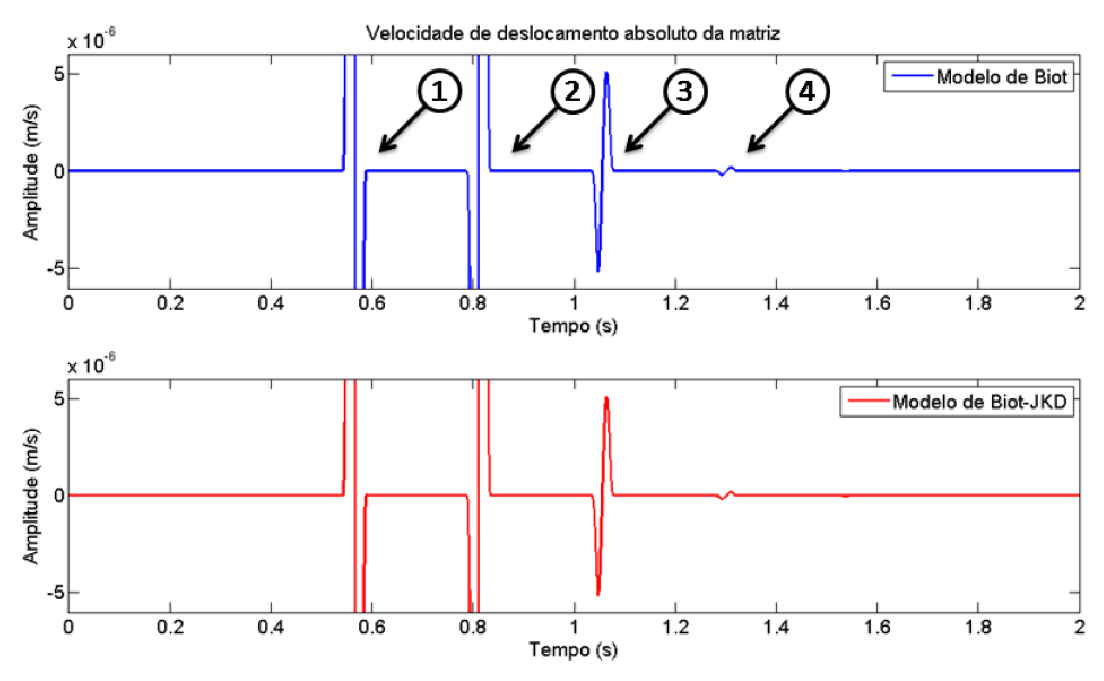
\includegraphics[scale=.65]{igor}
\caption{\textit{Velocidade de deslocamento da matriz para baixas frequ\^encias.}}
\label{fig.igor}
\end{figure}
Al\'em disso, no caso 1D a solu\c{c}\~ao do sistema de Biot pode ser formulada totalmente de maneira anal\'itica e expl\'icita. No caso 3D, todo o c\'odigo computacional s\'o pode ser implementado fazendo uso de opera\c{c}\~oes com matrizes, promovendo desafios em termos de aproxima\c{c}\~oes e instabilidades num\'ericas.


\section{Modelagem Matem\'atica e Num\'erica do Efeito Sismo-Magn\'etico}

Podemos observar uma an\'alise matem\'atica e num\'erica do efeito de indu\c{c}\~ao sismo-magn\'etica em \cite{mikhailenko_97}, onde \'e descrita a solu\c{c}\~ao simult\^anea de equa\c{c}\~oes el\'asticas com o acoplamento da for\c{c}a de Lorentz, e as equa\c{c}\~oes quasi-estacion\'arias de Maxwell com o acoplamento da velocidade de deslocamento do meio de propaga\c{c}\~ao das ondas. Tais sistemas de EDP's foram obtidos do modelo desenvolvido por \cite{Novacki_83} e foram transformados num sistema de EDO's utilizando transformadas finitas de Fourier.

O sistema de EDO's \'e escrito introduzindo uma matriz de vari\'aveis $A$, e a solu\c{c}\~ao num\'erica \'e obtida pelo m\'etodo de fatoriza\c{c}\~ao encontrado em \cite{Mikhailenko_89}, o qual utiliza a matriz de equa\c{c}\~oes de Riccati para a determina\c{c}\~ao das componentes $a_{ij}$. Tal abordagem n\~ao tem restri\c{c}\~oes computacionais se trabalhada com propaga\c{c}\~ao de ondas de alta frequ\^encia.

As simula\c{c}\~oes foram realizadas considerando ondas longitudinais, transversais e Rayleigh. Os resultados  mostraram, principalmente, que as primeiras chegadas das varia\c{c}\~oes geomagn\'eticas coincidiram com as chegadas dos tipos de ondas que as produziram. Essa coincid\^encia ocorreu para onda longitudinal, Rayleigh e para uma onda refletida na interface entre as camadas.

%\chapter{Elementos da F\'isica-Matem\'atica}

\section{EDP de uma Onda}
Segundo \cite{farlow_93}, a EDP de uma onda 
\begin{equation}\label{eq.edp_geral}
\frac{\partial^2\mathbf{f}(\mathbf{x},t)}{\partial\,t^2}=\norm{\mathbf{v}}^2\nabla^2\mathbf{f}(\mathbf{x},t)
\end{equation}
possui a solu\c{c}\~ao de D'Alembert
\begin{equation}
\mathbf{f}(\mathbf{x},t)=\mathbf{g}_1(\mathbf{x}-\mathbf{v}\,t)+\mathbf{g}_2(\mathbf{x}+\mathbf{v}\,t),
\end{equation}
onde $\mathbf{x}=(x,y,z)^\top$ representa o espa\c{c}o $\mathbb{R}^3$, $\mathbf{v}$ \'e a \textit{velocidade} de propaga\c{c}\~ao da onda, $(\mathbf{x}\pm\mathbf{v}\,t)$ \'e a \textit{fase} da onda, $\mathbf{g}_1$ \'e a propaga\c{c}\~ao da onda no semiespa\c{c}o positivo do eixo $x$ e $\mathbf{g}_2$ \'e a propaga\c{c}\~ao da onda no semiespa\c{c}o negativo do eixo $x$.

De acordo com \cite{chew}, ondas tridimensionais oriundas de fonte pontual se propagam em formato esferoidal mas localmente podem ser tratadas como ondas planas, principalmente para raios distantes da fonte. A onda esf\'erica, solu\c{c}\~ao da EDP \ref{eq.edp_geral}, pode ser representada pela superposi\c{c}\~ao de ondas planas atrav\'es da identidade de \textit{Weyl}, onde tal superposi\c{c}\~ao tamb\'em \'e solu\c{c}\~ao da EDP \ref{eq.edp_geral}, conforme \cite{weyl_19}.

No $\mathbb{R}^3$ o \textit{vetor de onda} $\mathbf{k}=(k_x,k_y,k_z)^\top$ \'e aquele que aponta na dire\c{c}\~ao de propaga\c{c}\~ao da onda e sua magnitude, denominada \textit{n\'umero de onda}, \'e definida como 
\begin{equation}
\norm{\mathbf{k}}=k=\frac{\omega}{\norm{\mathbf{v}}},
\end{equation}
onde $\omega$ \'e a frequ\^encia temporal. Desta forma, a fase da onda pode ser escrita em termos do vetor de onda e da frequ\^encia como $(\mathbf{k}\cdot\mathbf{x}-\omega\,t)$, e a solu\c{c}\~ao da equa\c{c}\~ao \ref{eq.edp_geral} pode ser reescrita como uma superposi\c{c}\~ao de ondas planas
\begin{equation}
\mathbf{f}(\mathbf{x},t)=\mathbf{A}\,\sum_{\mathbf{k},\omega}{e^{i\,(\mathbf{k}\cdot\mathbf{x}-\omega\,t)}},
\end{equation}
onde $\mathbf{A}$ \'e a \textit{amplitude} da onda.

Podemos verificar em \cite{White_Zhou_2006}, para o caso $\mathbb{R}^2$ o \textit{vetor de onda horizontal} \'e definido como $\mathbf{k}=(k_x,k_y)^\top$, o \textit{n\'umero de onda horizontal} e a \textit{vagarosidade horizontal} s\~ao, respectivamente,
\begin{equation}\label{eq.numero_onda_vagarozidade_horizontal}
k=\sqrt{k_x^2+k_y^2}\qquad\text{e}\qquad\gamma=\frac{k}{\omega}.
\end{equation}
A vagarosidade vertical \'e definida como
\begin{equation}
q_0=\frac{1}{v_z},
\end{equation}
onde $v_z$ \'e a componente vertical da velocidade. Denotando o \textit{n\'umero de onda vertical} por $k_z$, temos que a \textit{vagarosidade vertical} pode ser escrita como
\begin{equation}
q_0=\frac{k_z}{\omega}.
\end{equation}
Combinando as vagarosidades horizontal e vertical, temos
\begin{equation}\label{eq.vagarosidade_vertical}
\gamma^2+q_0^2=\frac{1}{\norm{\mathbf{v}}^2}\qquad\text{ou}\qquad q_0=\sqrt{\epsilon_0\mu_0-\gamma^2},
\end{equation}
j\'a que $\epsilon_0\mu_0=\frac{1}{\norm{\mathbf{v}}^2}$.

\section{Transformadas Laterais de Fourier}

Segundo \cite{butkov_88}, podemos definir as transformadas laterais de Fourier direta e inversa entre o espa\c{c}o bidimensional e o vetor de onda horizontal como
\begin{align}\label{eq.trans_fourier_1}
\mathbf{\widehat{f}}(k_x,k_y,z) &= \iint_{\mathbb{R}^2}\mathbf{f}(x,y,z)\,e^{-i(k_xx+k_yy)}dx\,dy\\\nonumber\\\label{eq.trans_fourier_2}
\mathbf{f}(x,y,z) &= \left(\frac{1}{2\,\pi}\right)^2\iint_{\mathbb{R}^2}\mathbf{\widehat{f}}(k_x,k_y,z)\,e^{i(k_xx+k_yy)}dk_xdk_y.
\end{align}
O s\'imbolo $\,\widehat{}\,$ denota a fun\c{c}\~ao no espa\c{c}o da transformada lateral de Fourier.

A propriedade da transformada de derivadas \'e a que mais nos interessa e, supondo $f$ uma fun\c{c}\~ao escalar de uma \'unica vari\'avel, essa propriedade pode ser descrita como  
\begin{align*}
\widehat{f'}(x)&=\int_{-\infty}^{\infty}f'(x)\,e^{-i\,k_xx}dx\\
&=f(x)\,e^{-i\,k_xx}|_{-\infty}^{\infty}-(-i\,k_x)\int_{-\infty}^{\infty}f(x)\,e^{-i\,k_xx}dx\\
&=i\,k_x\widehat{f}(k_x).
\end{align*}
Na passagem da segunda para a terceira igualdade utilizamos a hip\'otese bastante difundida em geof\'isica de que $f(x)\rightarrow 0$ quando $x \rightarrow \pm \infty $, a qual podemos observar em demonstra\c{c}\~oes de teoremas como, por exemplo, o toerema de \textit{Helmholtz} encontrado em \cite{griffiths}. 


\section{Rota\c{c}\~oes}

Segundo \cite{lang_1986}, podemos produzir uma rota\c{c}\~ao antihor\'aria em torno do eixo $z$ aplicando o operador linear
\begin{equation*}
\begin{pmatrix}
\cos\theta&-\sin\theta&0\\
\sin\theta&\cos\theta&0\\
0&0&1
\end{pmatrix},
\end{equation*}
onde $\theta$ \'e o \^angulo que um vetor est\'a sendo rotacionado. Como a geometria do nosso problema considera ondas se propagando na parte negativa do eixo $z$ (consideramos $z$ positivo no sentido descendente), para produzirmos uma rota\c{c}\~ao antihor\'aria devemos considerar o \^angulo $-\theta$, e com isso nossa matriz de rota\c{c}\~ao se torna
\begin{equation*}
\begin{pmatrix}
\cos\theta&\sin\theta&0\\
-\sin\theta&\cos\theta&0\\
0&0&1
\end{pmatrix},
\end{equation*}
lembrando a paridade das fun\c{c}\~oes seno e cosseno. Para promovermos uma rota\c{c}\~ao orientando a primeira coordenada  no sentido de propaga\c{c}\~ao das ondas horizontais, temos que $\theta$ ser\'a o \^angulo entre $(x,0,0)^\top$ e $(k_x,k_y,0)^\top$, e a matriz de rota\c{c}\~ao se torna
\begin{equation}\label{eq.operador_rotacao}
\Omega=
\begin{pmatrix}
\frac{k_x}{k}&\frac{k_y}{k}&0\\
-\frac{k_y}{k}&\frac{k_x}{k}&0\\
0&0&1
\end{pmatrix}.
\end{equation}
Para escrevermos novamente as equa\c{c}\~oes no sistema de coordenadas original, precisamos aplicar a rota\c{c}\~ao inversa. Para isso, basta inverter a matriz de rota\c{c}\~ao \ref{eq.operador_rotacao} mas, como se trata de uma matriz ortogonal, a inversa \'e a sua transposta. Assim, usaremos
\begin{equation}\label{eq.rotacao_inversa}
\Omega^\top=
\begin{pmatrix}
\frac{k_x}{k}&-\frac{k_y}{k}&0\\
\frac{k_y}{k}&\frac{k_x}{k}&0\\
0&0&1
\end{pmatrix}.
\end{equation}


A rota\c{c}\~ao de um tensor $\tau$ \'e dada por 
\begin{equation}\label{eq.rotacao_tensor}
\tilde{\tau}=\Omega\,\tau\,\Omega^\top,
\end{equation}
e sua rota\c{c}\~ao inversa \'e dada por
\begin{equation}\label{eq.rot_inver_tensor}
\tau=\Omega^\top\tilde{\tau}\,\Omega.
\end{equation}


\section{A fun\c{c}\~ao $\delta$ de Dirac}\label{sec.dirac}

Em algumas aplica\c{c}\~oes f\'isicas pode ser necess\'ario trabalhar com conceito de um pulso de dura\c{c}\~ao infinitamente curta. De acordo com \cite{butkov_88}, podemos tomar o exemplo de um corpo colocado em movimento, a partir do repouso, atrav\'es de um golpe instant\^aneo que faz o mesmo adquirir um momento igual \`a impuls\~ao $I$ do choque, ou seja,
\begin{equation}
I=\int_{t_0}^{t_0+\Delta\,t}f(t)dt,
\end{equation}
onde $f(t)$ \'e a for\c{c}a e $\Delta\,t$ \'e o tempo de a\c{c}\~ao da for\c{c}a. A implus\~ao \'e um n\'umero finito e sua altera\c{c}\~ao ocorre instantaneamente, pois $\Delta\,t$ \'e um n\'umero muito pequeno. Assim, temos que a for\c{c}a deveria ter valor infinito durante o golpe e nula nos outros instantes, conforme o gr\'afico da figura \ref{fig.dirac}.
\begin{figure}
\centering
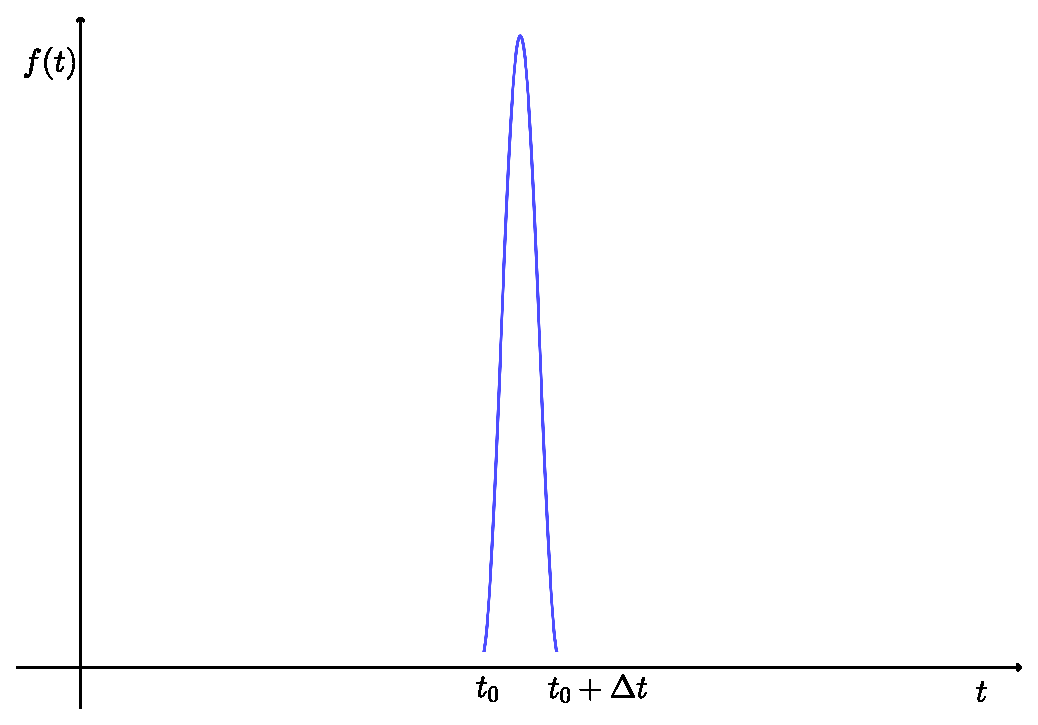
\includegraphics[scale=.6]{dirac_function}
\caption{\textit{Representa\c{c}\~ao de uma fun\c{c}\~ao fortemente concentrada.}}
\label{fig.dirac}
\end{figure}
A fim de facilitar v\'arias opera\c{c}\~oes da f\'isica-matem\'atica, Dirac prop\^os a introdu\c{c}\~ao da chamada fun\c{c}\~ao $\delta(x)$, que pode representar uma fun\c{c}\~ao infinitamente concentrada e \'e dada simbolicamente por
\begin{empheq}[left={\delta(x)=\empheqlbrace}]{align*}
0\,,&\quad\text{se}\quad x\neq 0\\
\infty\,,&\quad\text{se}\quad x=0
\end{empheq}
e $\delta$ deve satisfazer a seguinte condi\c{c}\~ao
\begin{equation}\label{eq.condicao_dirac}
\int_{-\infty}^{\infty}\delta(x)\,dx=1.
\end{equation}
Sendo $f$ uma fun\c{c}\~ao cont\'inua qualquer, a utilidade da fun\c{c}\~ao $\delta$ consiste em determinar o valor de 
\begin{equation}
\int_{-\infty}^{\infty}\delta(x)\,f(x)\,dx
\end{equation}
substituindo os limites de integra\c{c}\~ao por $-\epsilon$ e $\epsilon$, onde $\epsilon$ \'e um n\'umero positivo infinitesimalmente pr\'oximo de zero. Tal substitui\c{c}\~ao se justifica pois $\delta=0$ se $x\neq0$ e teremos uma aproxima\c{c}\~ao para o valor dessa integral. Assim, usando a defini\c{c}\~ao de $\delta$, a condi\c{c}\~ao \ref{eq.condicao_dirac} e a continuidade de $f$, temos
\begin{align*}
\int_{-\infty}^{\infty}\delta(x)\,f(x)\,dx&=\int_{-\infty}^{-\epsilon}\delta(x)\,f(x)\,dx+\int_{-\epsilon}^{\epsilon}\delta(x)\,f(x)\,dx+\int_{\epsilon}^{\infty}\delta(x)\,f(x)\,dx\\
&=\int_{-\epsilon}^{\epsilon}\delta(x)\,f(x)\,dx\\
&\approx\,f(0)\int_{-\epsilon}^{\epsilon}\delta(x)\,dx\\
&=f(0).
\end{align*}
Desta forma podemos representar a aplica\c{c}\~ao de uma fun\c{c}\~ao fortemente concentrada, incluindo a representa\c{c}\~ao de uma fonte pontual de onda s\'ismica que \'e de interesse geof\'isico, como veremos na subse\c{c}\~ao \ref{sec.presenca_fonte}.

\section{Fun\c{c}\~ao de Bessel de Primeira Esp\'ecie}

De acordo com \cite{butkov_88}, sendo $f(x)$ uma fun\c{c}\~ao qualquer, podemos escrever a equa\c{c}\~ao diferencial ordin\'aria de Bessel na forma
\begin{equation}
\frac{d^2f}{dx}+\frac{1}{x}\frac{df}{dx}+\left(1-\frac{m^2}{x^2} \right)\,f=0,
\end{equation}
onde, estudando o caso geral temos que $m$ \'e um n\'umero real arbitr\'ario que pode ser considerado n\~ao-negativo, mas no nosso trabalho vamos considerar $m$ inteiro positivo. A equa\c{c}\~ao acima \'e a EDO de Bessel de ordem $m$, suas solu\c{c}\~oes s\~ao conhecidas como fun\c{c}\~oes cil\'indricas e entre elas est\~ao as fun\c{c}\~oes de Bessel. Expandindo a fun\c{c}\~ao $f(x)$ numa s\'erie de \textit{Frobenius} e substituindo-a  na EDO de Bessel podemos deduzir que a solu\c{c}ao \'e dada por
\begin{equation}\label{eq.funcao_bessel_1}
J_m(x)=\sum_{j=0}^{\infty}(-1)^j\frac{x^{m+2\,j}}{j!\,\Gamma\,(m+j+1)\,2^{m+2\,j}}.
\end{equation}
A fun\c{c}\~ao $\Gamma$ \'e uma fun\c{c}\~ao fatorial de vari\'avel real com representa\c{c}\~ao na forma integral dada por
\begin{equation*}
\Gamma(\xi)=\int_0^\infty t^{\xi-1}e^tdt,\qquad x>0.
\end{equation*}
Como estamos trabalhando com $m$ inteiro positivo, a fun\c{c}\~ao $\Gamma(\xi)$ \'e dada simplesmente por $(\xi-1)!$. Assim, a express\~ao \ref{eq.funcao_bessel_1} passa a ser escrita como
\begin{equation}\label{eq.funcao_bessel_2}
J_m(x)=\sum_{j=0}^{\infty}\frac{(-1)^j}{j!\,(m+j)!}\left(\frac{x}{2}\right)^{m+2\,j}
\end{equation}
e \'e chamada fun\c{c}\~ao de Bessel de primeira esp\'ecie de ordem $m$.

\section{Transformadas de Hankel}\label{sec.trans_hankel}
A transformada de Hankel utiliza as fun\c{c}\~oes de Bessel para transformar um sistema de coordenadas $\mathbf{x}$ para outro $\pmb{\xi}$. De acordo com \cite{baruch_2013}, assumindo que $f$ seja uma fun\c{c}\~ao radial, ou seja, que depende apenas da magnitude $x$ de $\mathbf{x}$, umas das defini\c{c}\~oes da transformada de Hankel \'e dada por
\begin{equation*}
\mathcal{B}_m[f(x)](\xi)=\int_0^\infty x\,J_m(x\,\xi)\,f(x)\,dx.
\end{equation*}
E a transformada inversa, considerando $\xi=\norm{\pmb{\xi}}$, \'e
\begin{equation*}
\mathcal{B}^{-1}_m[F(\xi)](x)=\int_0^\infty \xi\,J_m(x\,\xi)\,F(\xi)\,d\xi,
\end{equation*}
onde $J_m$ \'e uma fun\c{c}\~ao de Bessel de primeira esp\'ecie de ordem $m$, conforme visto na subse\c{c}\~ao anterior.











%\chapter{Fundamentos de eletromagnetismo}\label{sec.fund_eletr}

\section{Introdução}

\section{Fatos experimentais}

\subsection{Lei de Gauss para os fluxos elétrico e magnético}
De acordo com \cite{jackson_classical_1999} e \cite{sommerfeld_52} , os conceitos, definições e resultados em eletromagnetismo clássico partem das experiências de Cavendish e Coulomb no final do Séc. $XVIII$. A partir desses experimentos foi estabelecida a Lei de Coulomb
\begin{equation}\label{eq.forc_elet}
\textbf{F}=k\,\frac{q_1\,q_2}{||\textbf{x}_1-\textbf{x}_2||^2}\frac{\textbf{x}_1-\textbf{x}_2}{||\textbf{x}_1-\textbf{x}_2||},
\end{equation}
onde $q_i$ são as cargas elétricas (campos escalares) presentes nos pontos $\textbf{x}_i$, respectivamente, $k$ (campo escalar) é uma constante de proporcionalidade cujo valor depende do sistema de unidades de medida adotado, $||\textbf{x}_1-\textbf{x}_2||^2$ é a distância euclidiana entre as cargas e $\textbf{F}$ é a força elétrica exercida pela carga $q_1$ sobre a carga $q_2$. As notações em negrito representam campos vetorias pertencentes ao espaço $\mathbb{R}^3$, e o vetor normal que fornece a direção de interação entre as cargas é dado por $(\textbf{x}_1-\textbf{x}_2)/||\textbf{x}_1-\textbf{x}_2||$.

O campo elétrico $\textbf{E}$ é definido como sendo a força elétrica por unidade de carga em um determinado ponto que contém a carga de prova $q_2$, portanto é uma função vetorial que depende da posição da carga de prova em relação à carga fonte $q_1$, ou seja,
\begin{equation}\label{eq.camp_elet}
\textbf{E}=\lim_{q_2\to 0}\frac{\textbf{F}}{q_2}.
\end{equation}
A carga de prova foi tomada infinitesimalmente pequena para que o campo gerado por ela não perturbe a carga fonte. Experimentalmente, tanto a direção da força como a razão entre a força e a quantidade de carga vão se tornando constantes à medida que a quantidade de carga se torna cada vez menor, definindo a magnitude e a direção do campo elétrico. No SI, a unidade de medida de carga é o \textit{coulomb} $(C)$, o campo elétrico é o \textit{newton/coulomb} $(N/C)$ ou o \textit{volt/metro} $(V/m)$, e a constante $k=(4\pi\,\epsilon_0)^{-1}$ onde $\epsilon_0\simeq8.854\times10^{-12}$ é a \textit{permissividade elétrica no vácuo} medida em \textit{farad/m} $(F/m)$.

Substituindo a equação \ref{eq.camp_elet} em \ref{eq.forc_elet} temos que o campo elétrico agindo num ponto $\textbf{x}$ qualquer devido a uma carga $q_1$ no ponto $\textbf{x}_1$ é
\begin{equation}\label{eq.campo_eletrico}
\textbf{E}=k\,\frac{q_1}{||\textbf{x}_1-\textbf{x}||^2}\frac{\textbf{x}_1-\textbf{x}}{||\textbf{x}_1-\textbf{x}||},
\end{equation}
como podemos observar na figura \ref{fig.camp_eletr} simulando um sistema de coordenadas qualquer.
\begin{figure}[!htb]
\centering
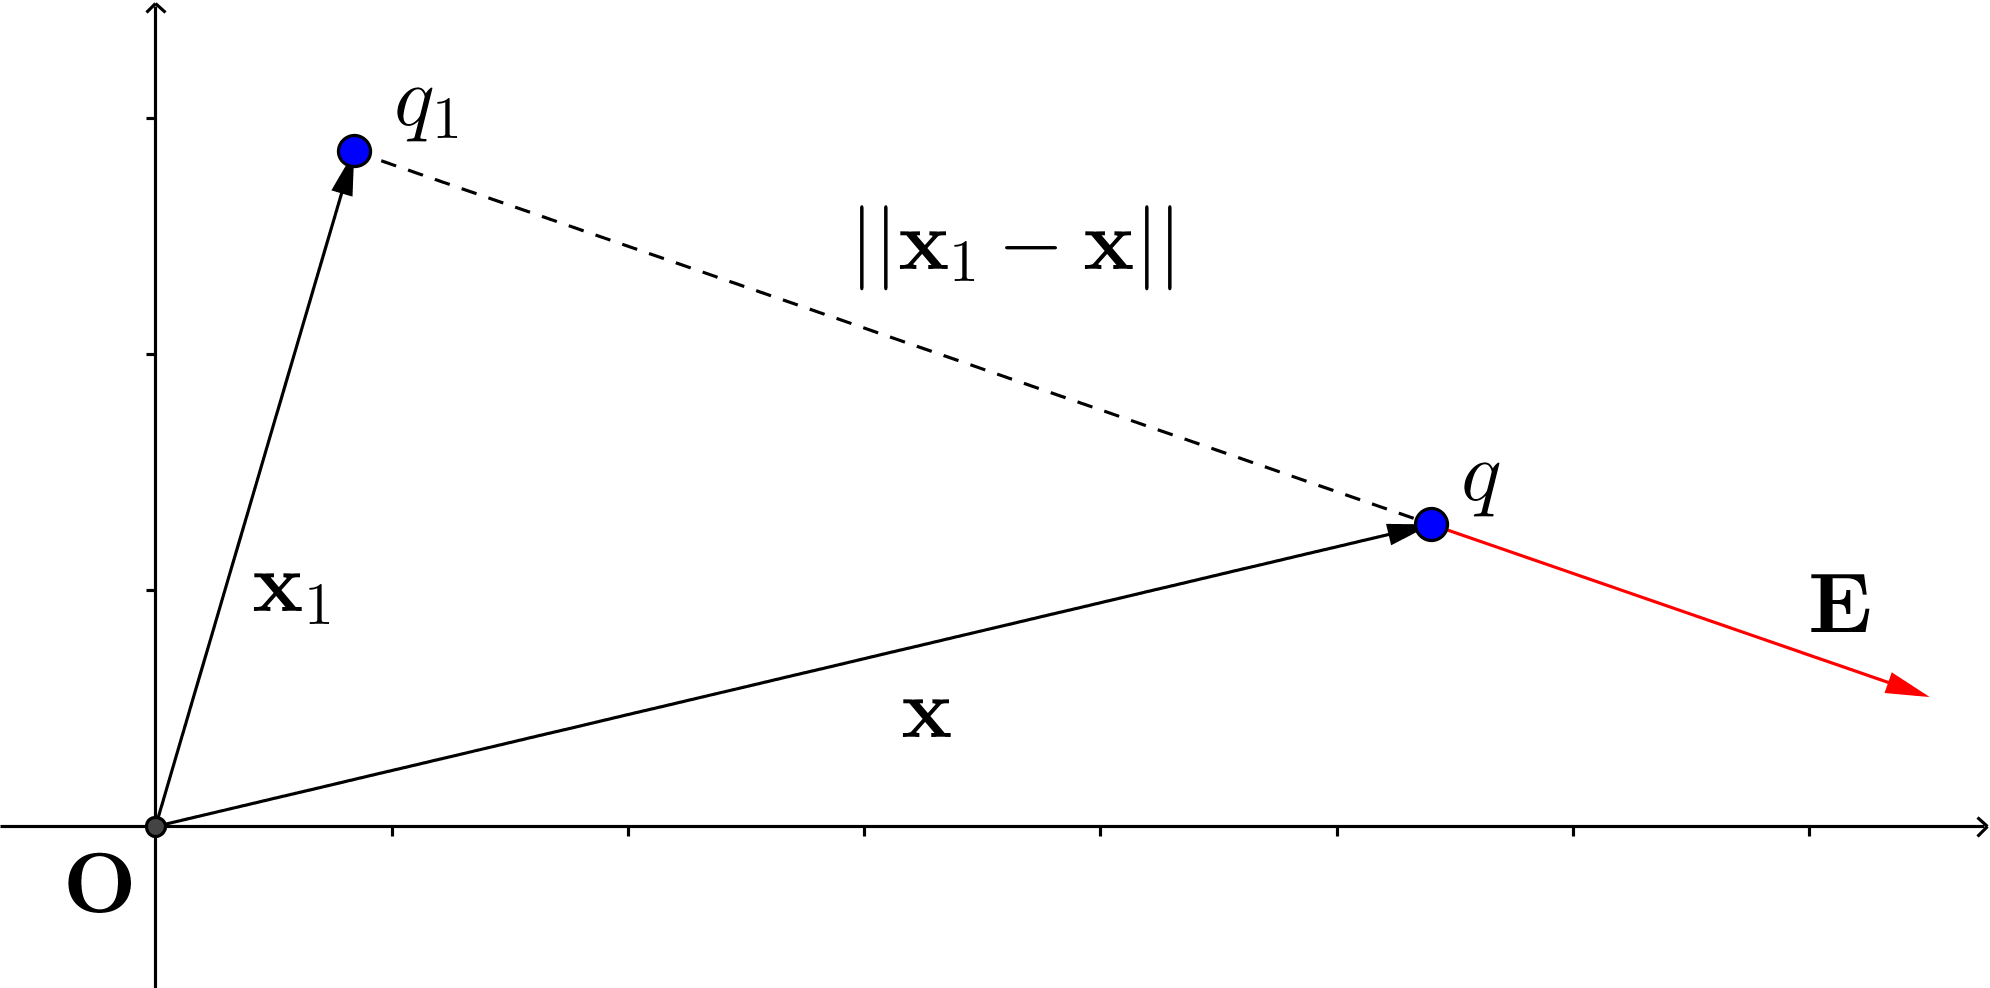
\includegraphics[scale=1.5]{camp_elet}
\caption{\textit{Exemplificação da interação entre cargas elétricas devido à geração, em função de $q_1$, de um campo elétrico. A força elétrica $\textbf{F}$ atuando numa carga qualquer $q$ tem mesma direção do campo elétrico $\textbf{E}$, com mesmo sentido ou sentido oposto conforme a carga $q$ é positiva ou negativa, respectivamente.}}
\label{fig.camp_eletr}
\end{figure}

%\begin{figure}[!htb]
%\centering
%\subfloat{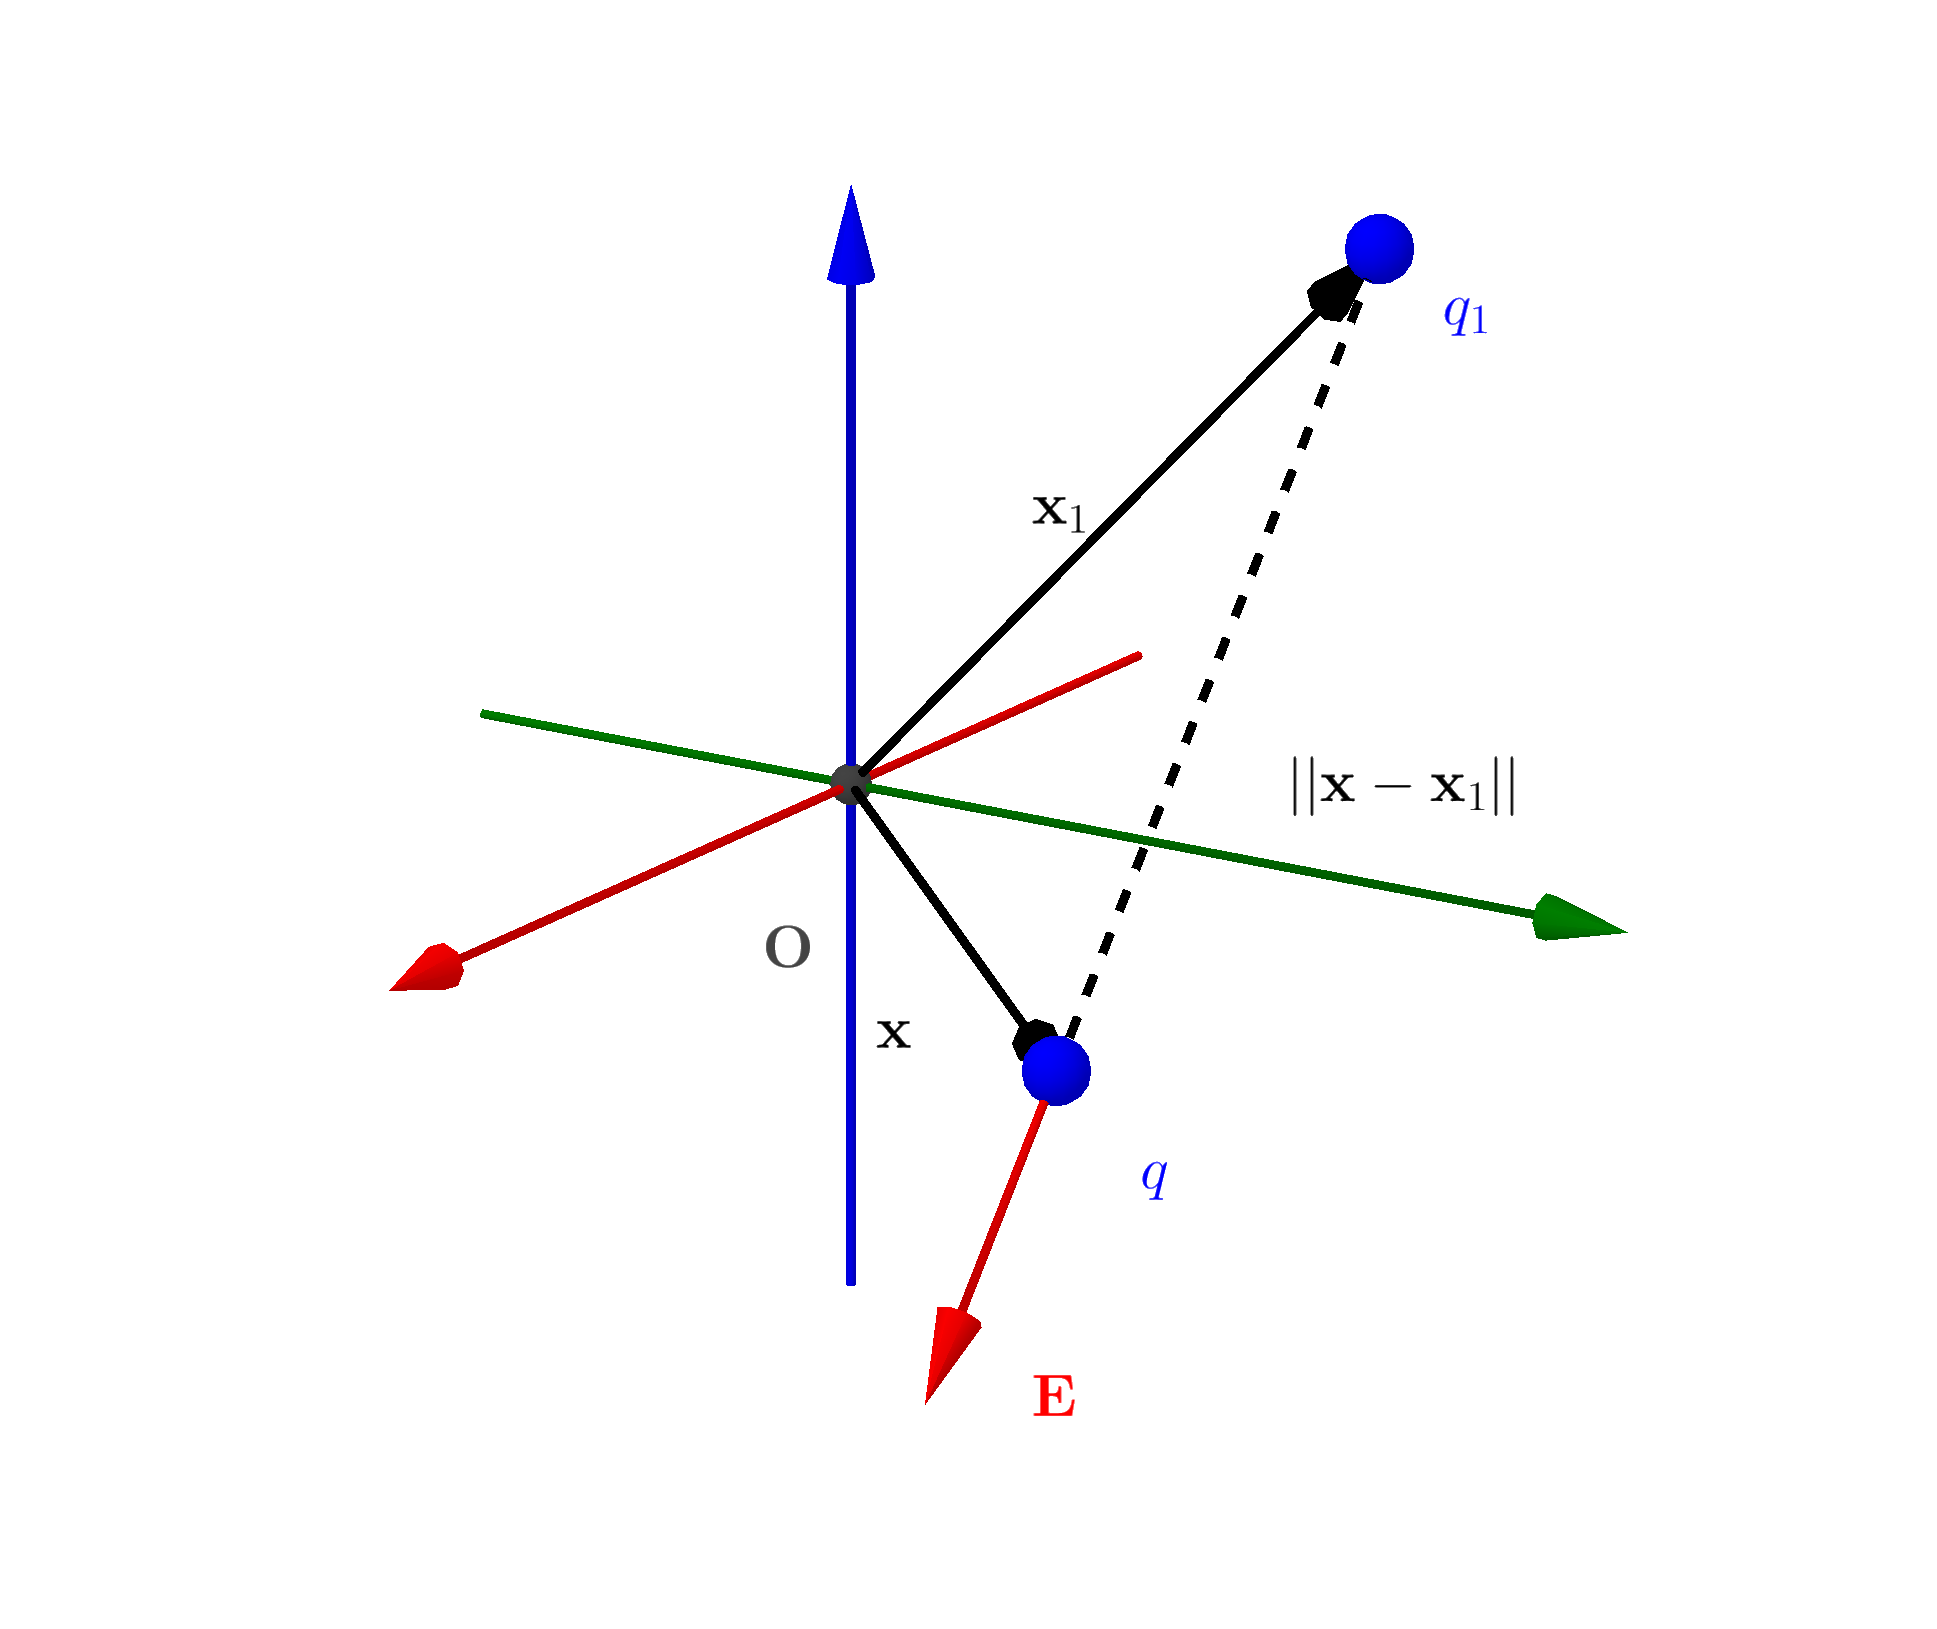
\includegraphics[scale=1]{camp_elet_3D}}
%\subfloat{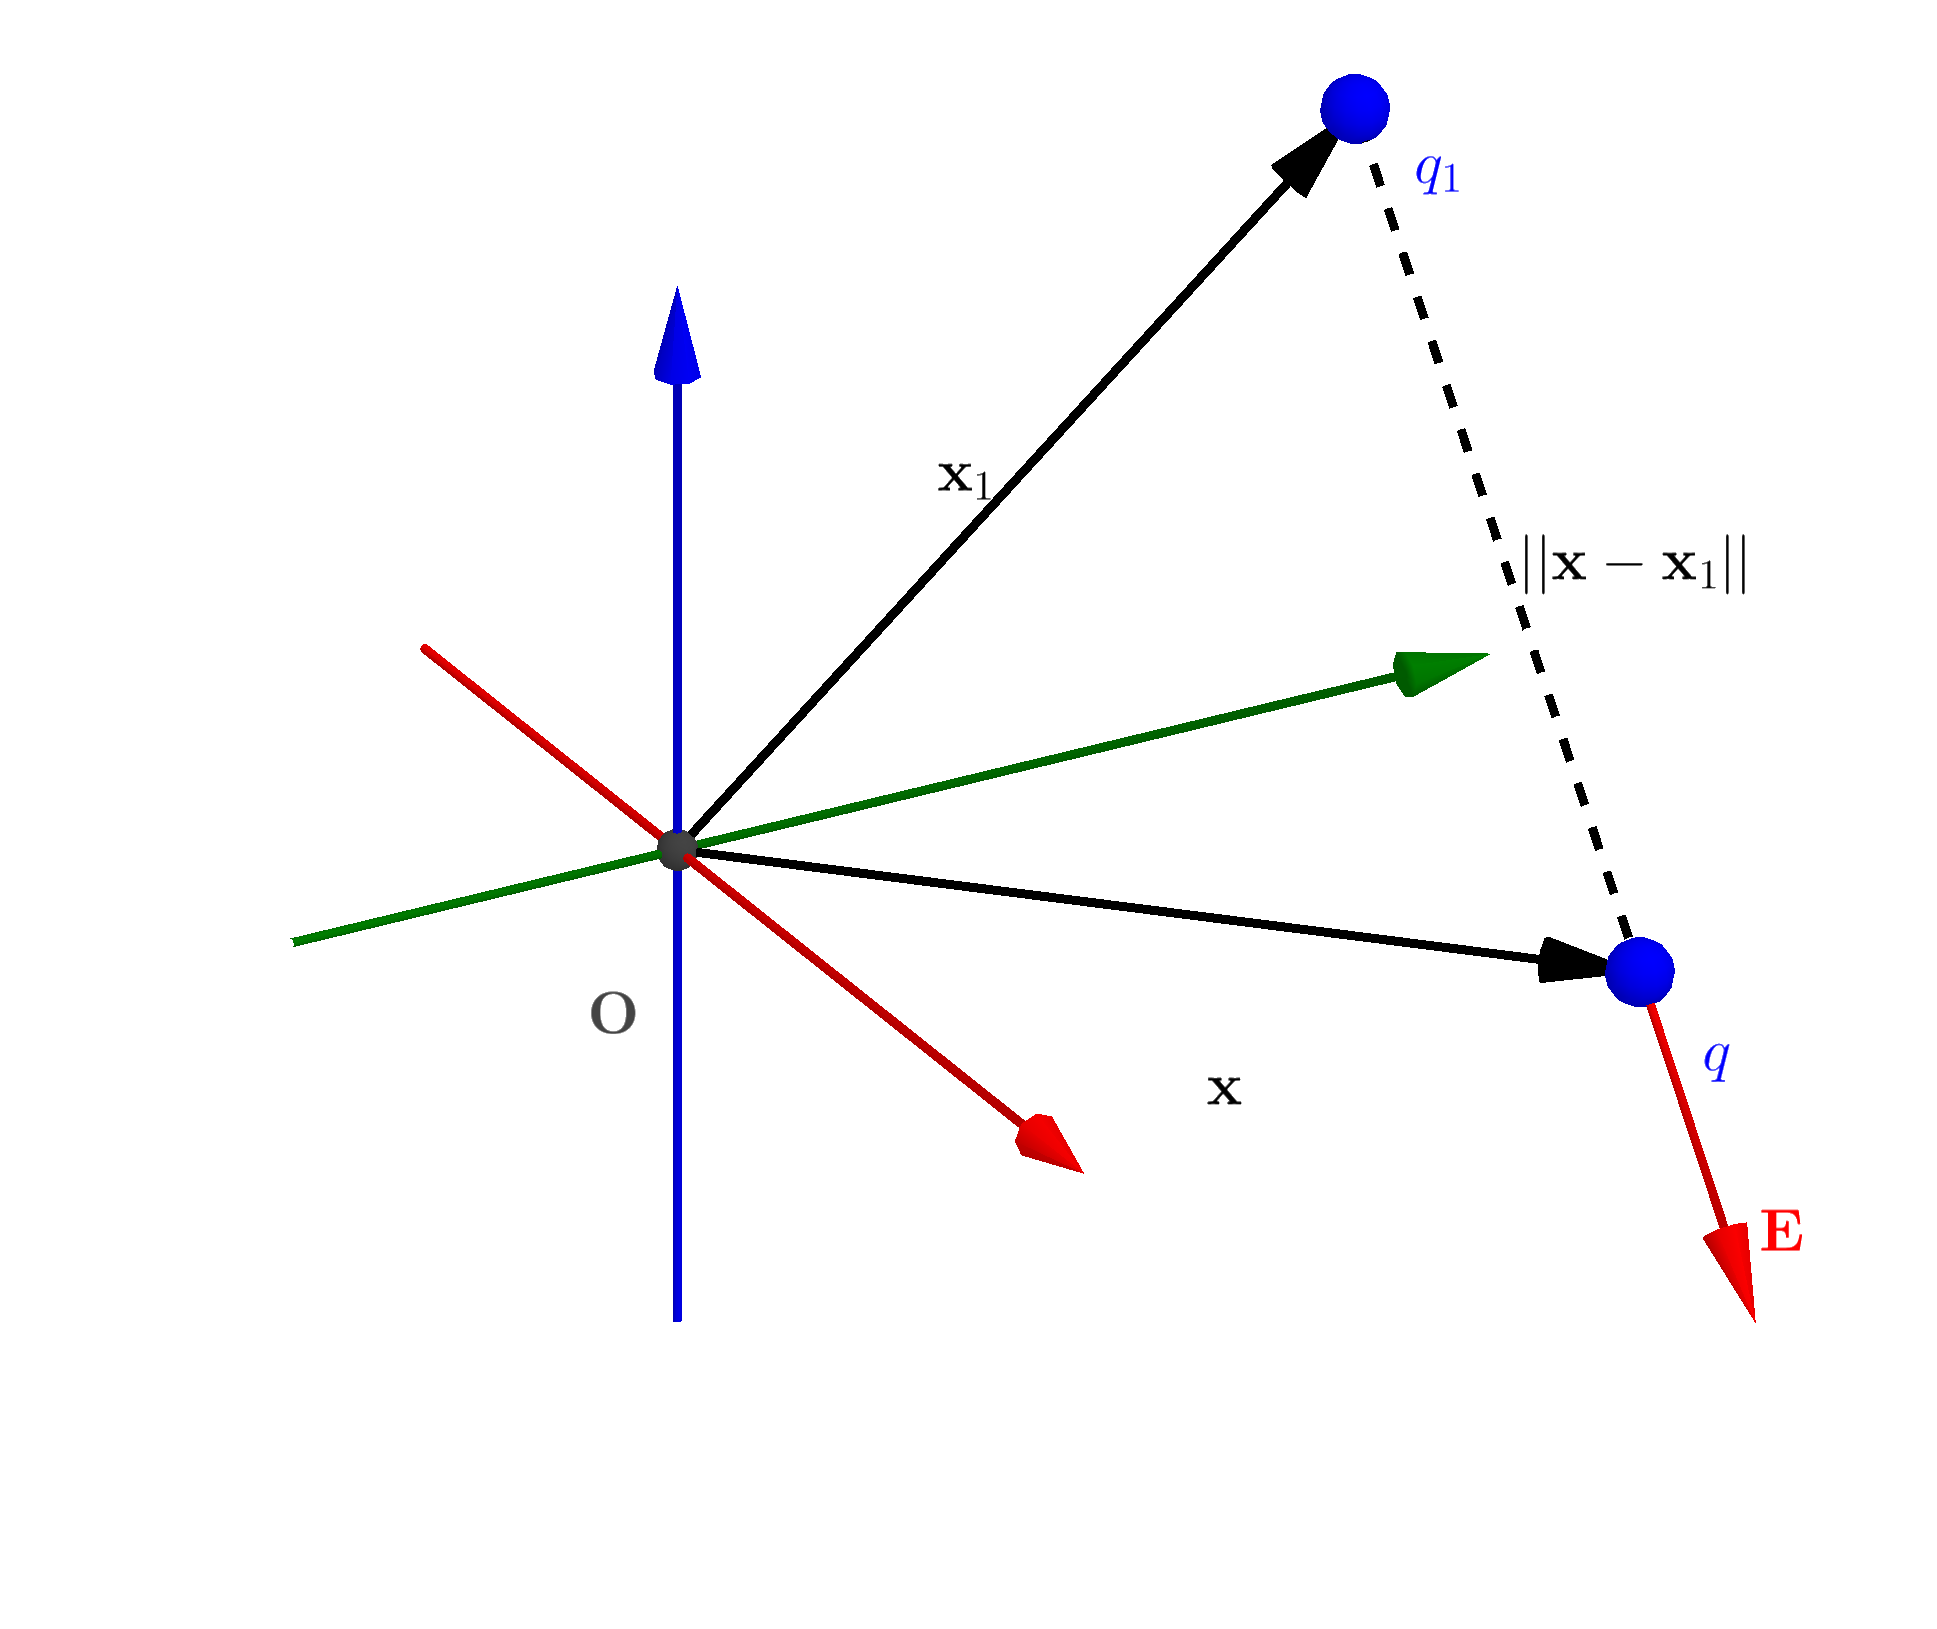
\includegraphics[scale=1]{camp_elet_3D2}}
%\caption{}
%\label{fig.mossul}
%\end{figure}

Num sistema com mais de uma carga fonte produzindo campos elétricos, foi observado experimentalmente que o campo elétrico total atuando num ponto $\textbf{x}$ é simplesmente o somatório dos campos produzidos por cada carga, o que ficou conhecido como a \textit{Superposição Linear} e pode ser expressada na forma
\begin{equation*}
\textbf{E}=k\,\sum_{i=1}^{n}q_i\,\frac{\textbf{x}_i-\textbf{x}}{||\textbf{x}_i-\textbf{x}||^3}.
\end{equation*} 
O campo elétrico devido a um pequeno número de cargas pode ser calculado a partir do princípio da superposição linear. Mas se temos uma quantidade muito grande de cargas num determinado volume $V$, devemos calcular a \textit{densidade volumétrica de carga} $\rho$ num volume infinitesimal situado em $\textbf{x}_0$ e em seguida integrar sobre o volume $V$ para obter a quantidade total de carga $Q$. A densidade de carga é definida por
\begin{equation*}
\rho(\textbf{x}_0)=\lim_{\Delta V_i \to 0}\frac{\Delta q_i}{\Delta V_i}=\frac{d\,q}{d\,V},
\end{equation*}
medida, no SI, em $C/m^3$. A quantidade total de carga $Q=\sum_i \Delta\,q_i$ no volume $V$ é
\begin{equation*}
Q=\int_{V}\rho(\textbf{x}_0)\,dV.
\end{equation*}

O \textit{fluxo elétrico} é definido como a quantidade linhas do campo elétrico que atravessam uma dada superfície, e é dado pela equação
\begin{equation*}
\Phi_\textbf{E}=\textbf{E}\cdot\textbf{A}. 
\end{equation*} 
O \textit{vetor área} é definido como a magnitude da área da superfície atravessada apontando na direção do vetor normal à superfície, $\textbf{A}=A\,\textbf{n}$, e estamos considerando um campo elétrico uniforme $\textbf{E}$ que se desloca na direção $\textbf{n}$, ou seja, é perpendicular à superfície $A$ como podemos observar na figura \ref{fig.flux_ele}.
\begin{figure}[!htb]
\centering
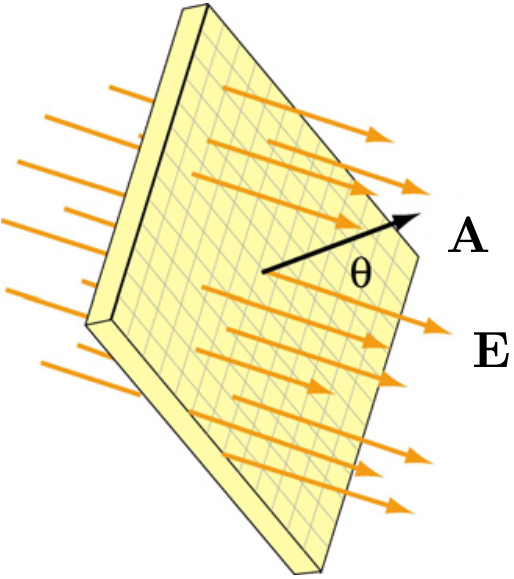
\includegraphics[scale=.5]{campo_area}
\caption{\textit{Fluxo elétrico, linhas de campo elétrico passando através de uma superfície.}}
\label{fig.flux_ele}
\end{figure}
Mas se o campo elétrico se propaga formando um ângulo $\theta$ com o vetor normal da superfície, então o fluxo elétrico é dado por
\begin{equation*}
\Phi_\textbf{E}=\textbf{E}\cdot\textbf{A}=E\,A\,\cos\theta,
\end{equation*}
com $E=\textbf{E}\cdot\textbf{n}$ sendo a componente do campo elétrico na direção $\textbf{n}$. Em geral uma superfície pode ser curva e estamos interessados numa superfície \textit{fechada}, ou seja, aquela que engloba um determinado volume, o qual contém uma carga elétrica. Tomando uma área bem pequena dessa superfície, $\Delta\textbf{A}_i$, o campo elétrico pode ser variável em cada parte da superfície e nessas condições temos que o fluxo nessa pequena região é dado por
\begin{equation*}
\Delta\,\Phi_\textbf{E}=\textbf{E}_i\cdot\Delta\,\textbf{A}_i.
\end{equation*}
O fluxo positivo atravessando toda a superfície de dentro para fora é calculado tomando o limite quando $\Delta\textbf{A}_i\to 0$ e aumentando infinitamente a quantidade dessas pequenas áreas
\begin{equation}\label{eq.fluxo_eletr}
\Phi_\textbf{E}=\lim_{i\to\infty}\sum_i\textbf{E}_i\cdot\textit{d}\textbf{A}_i=\int\int_S\textbf{E}\cdot\textit{d}\textbf{A}.
\end{equation}

Considere uma carga pontual positiva $q$ localizada no centro de uma esfera imaginária de raio $r$, onde essa carga produz um campo elétrico que aponta na direção radial conforme a figura \ref{fig.esfe_gauss}. Sabemos que a área da superfície dessa esfera é dada por $A=4\pi\,r^2$ e que, segundo a equação \ref{eq.campo_eletrico}, a magnitude do campo elétrico em qualquer ponto da superfície esférica é
\begin{equation*}
E=\frac{q}{4\pi\epsilon_0\,r^2},
\end{equation*}
assim o fluxo elétrico é calculado usando a equação \ref{eq.fluxo_eletr}.
\begin{align*}
\Phi_\textbf{E}&=\int\int_S\textbf{E}\cdot\textit{d}\textbf{A}\\
&=\int\int_S\textbf{E}\cdot\textbf{n}\,\textit{d}A\\
&=E\,\int\int_S\textit{d}A\\
&=E\,A\\
&=\frac{q}{4\pi\epsilon_0\,r^2}\,4\pi\,r^2\\
&=\frac{q}{\epsilon_0}.
\end{align*}
Na demonstração acima escolhemos uma esfera como \textit{superfície Gaussiana} mas, introduzindo o conceito de \textit{ângulo sólido}, vemos que a demonstração é válida para qualquer superfície fechada, utilizada em aplicações que apresentem mais ou menos alguma simetria (esférica, planar ou cilíndrica). Para mais detalhes consultar \cite{jackson_classical_1999}. Assim, concluímos que o fluxo elétrico através de uma superfície fechada que apresente mais ou menos alguma simetria é diretamente proporcional à quantidade de carga enclausurada pela superfície. Matematicamente, a \textit{lei de Gauss} para o fluxo elétrico é
\begin{equation*}
\Phi_\textbf{E}=\int\int_S\textbf{E}\cdot\textit{d}\textbf{A}=\frac{q}{\epsilon_0}.
\end{equation*}
\begin{figure}[!htb]
\centering
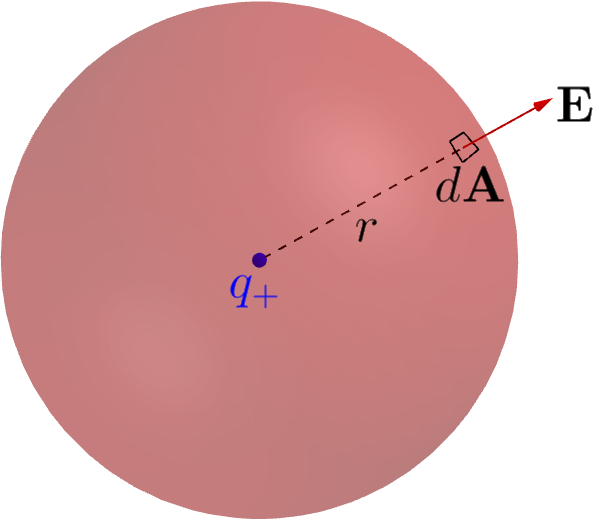
\includegraphics[scale=.3]{esfera_gaussiana}
\caption{\textit{Esfera Gaussiana enclausurando uma carga positiva $q$. Nessas condições, o ângulo entre o vetor campo elétrico e o vetor normal à superfície infinitesimal $d\textbf{A}$ é zero.}}
\label{fig.esfe_gauss}
\end{figure}

Uma carga elétrica produz um campo elétrico, e de maneira similar uma barra magnética, ou ímã, produz um \textit{campo magnético} $\textbf{B}$. Um ímã possui um polo norte de onde partem as linhas de campo magnético e um polo sul por onde as linhas de campo magnético retornam ao ímã (figura \ref{fig.barras_mag}). Diferentemente das cargas elétricas que são observadas isoldamente na natureza, os dois polos magnéticos sempre aparecem aos pares, ou seja, monopolos magnéticos não existem isoladamente apesar de a suposição de sua existência ser de interesse teórico. Assim, sempre que um ímã é fracionado, mesmo que em partes muito elementares, o resultado sempre será um novo ímã com dois polos magnéticos conforme a figura \ref{fig.barras_mag}.
\begin{figure}[!htb]
\centering
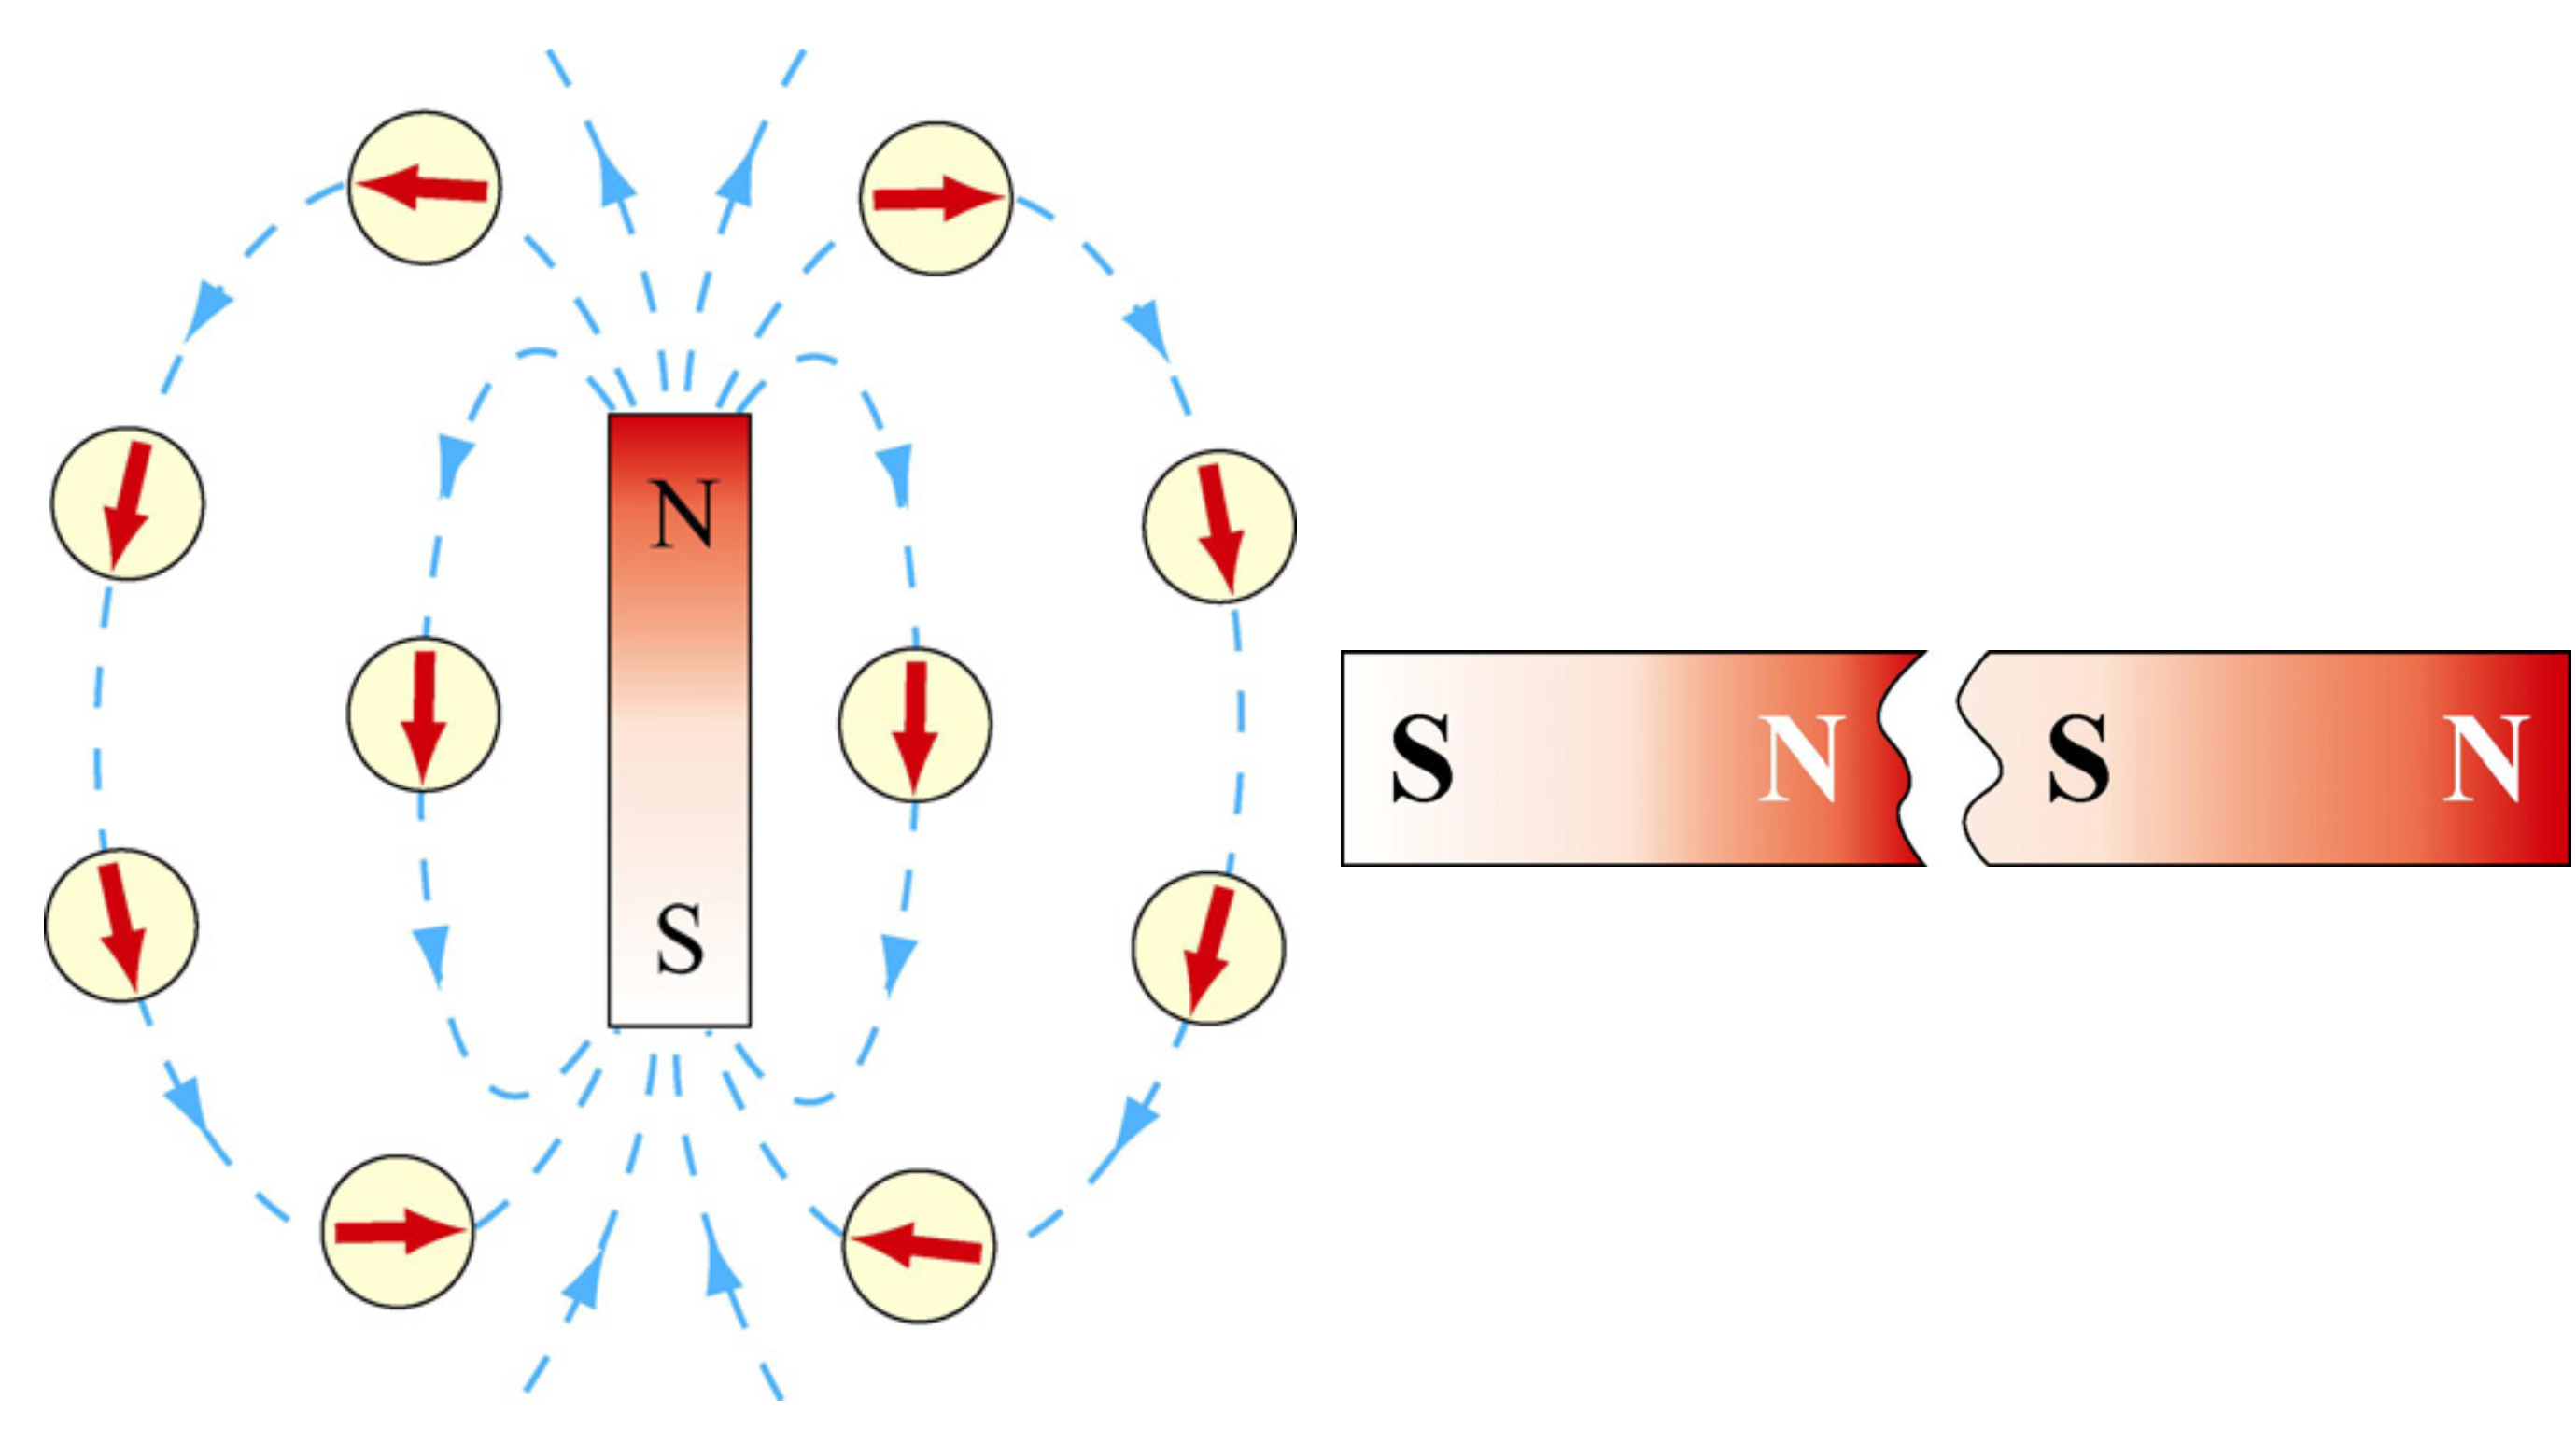
\includegraphics[scale=.7]{barras_magn}
\caption{\textit{Barras magnéticas onde polos de mesmo sinal se repelem e polos de sinais contrários se atraem.}}
\label{fig.barras_mag}
\end{figure}
Como não existem monopolos magnéticos, o campo magnético deve ser definido de forma diferente do campo elétrico, e experimentalmente foram observadas algumas características relacionadas ao movimento de uma carga elétrica $q$ com velocidade $\textbf{v}$ num campo magnético $\textbf{B}$:
\begin{itemize}
\item a magnitude da força magnética $\textbf{F}_B$ é proporcional à $v$, $B$ e $q$, onde $v$ e $B$ são as magnitudes da velocidade e do campo magnético respectivamente,
\item a direção de $\textbf{F}_B$ é perpendicular ao plano formado por $\textbf{v}$ e $\textbf{B}$,
\item $\textbf{F}_B$ é proporcional ao $\sin\theta$, o ângulo formado por $\textbf{v}$ e $\textbf{B}$. Se $\textbf{v}$ e $\textbf{B}$ são paralelos então $\textbf{F}_B=0$, e
\item o sentido de $\textbf{F}_B$ depende do sinal da carga $q$.
\end{itemize}
Essas observações são ilustradas na figura \ref{fig.froca_mag_veloc} e a força magnética é definida como
\begin{equation*}
\textbf{F}_B=q\textbf{v}\times\textbf{B}.
\end{equation*}
\begin{figure}[!htb]
\centering
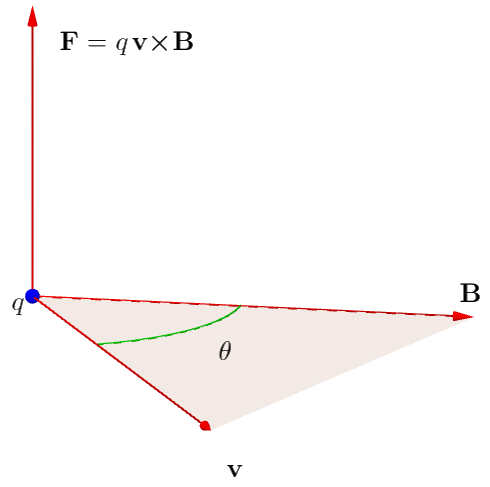
\includegraphics[scale=.4]{forca_camp_mag_veloc}
\caption{\textit{Força magnética agindo numa carga elétrica que se desloca num campo magnético.}}
\label{fig.froca_mag_veloc}
\end{figure}
Teoricamente, poderíamos tentar determinar a lei de Gauss para o fluxo magnético com o mesmo procedimento aplicado ao fluxo elétrico e obter
\begin{equation*}
\Phi_\textbf{B}=\int\int_S\textbf{B}\cdot\textit{d}\textbf{A}=\frac{q_m}{\mu_0},
\end{equation*} 
onde $q_m$ é a carga magnética (suposto monopolo magnético) enclausurado pela superfície Gaussiana, $B$ é o campo magnético e $\mu_0$ é a \textit{permeabilidade magnética no vácuo} com valor $\mu_0=4\,\pi\times 10^{-7} T.m/A$. No entanto, não foi constatada a existência de qualquer carga magnética isolada mesmo após muitos esforços. Como $q_m=0$, temos que a lei de Gauss para o magnetismo é
\begin{equation}\label{eq.gauss_flux_mag}
\Phi_\textbf{B}=\int\int_S\textbf{B}\cdot\textit{d}\textbf{A}=0.
\end{equation}
Conforme podemos ver na figura tal, a equação \ref{eq.gauss_flux_mag} implica que a quantidade de linhas do campo magnético saindo da superfície é igual à quantidade que está entrando, ou seja, não há uma origem isolada e um término isolado para o fluxo magnético como há para o fluxo elétrico. Outro problema é que a barra imantada atravessa a superfície que, de acordo com a hipóteses da lei de Gauss, deveria ser fechada.
\begin{figure}[!htb]
\centering
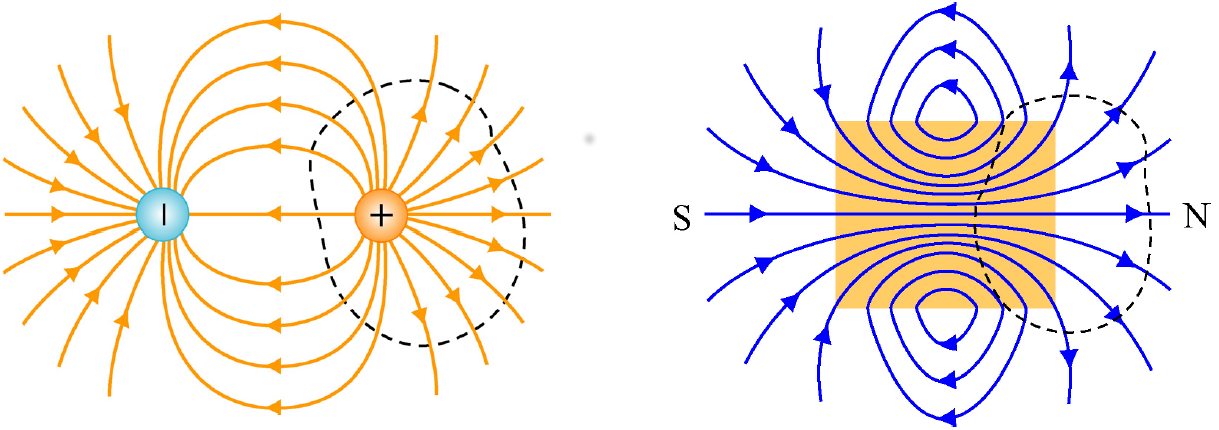
\includegraphics[scale=.3]{flux_ele_mag}
\caption{\textit{As linhas do campo magnético que emanam do polo norte do ímã em direção ao polo sul retornam para dentro da superfície Gaussiana descrevendo um laço fechado.}}
\label{fig.flux_elet_magn}
\end{figure}

\subsection{A Lei de Ampère}
Correntes elétricas podem ser produzidas por cargas elétricas que se movem num fio condutor. Essas correntes elétricas são fontes de campos magnéticos $d\,\textbf{B}$, num determinado ponto $x$, e que podem ser calculados em função da corrente $I$ num intervalo infinitesimal $d\,\textbf{l}$ do fio. Visualização na figura \ref{fig.corrente_fio}. A fonte de corrente infinitesimal é dada por $I\,d\,\textbf{l}$ e $r$ é a distância entre o ponto de aplicação do campo magnético e a fonte de corrente infinitesimal. O vetor $\textbf{n}$ é o vetor normal que aponta na direção de $x$ e o vetor $d\,\textbf{l}$ aponta na direção e sentido da corrente $I$. 
\begin{figure}
\centering
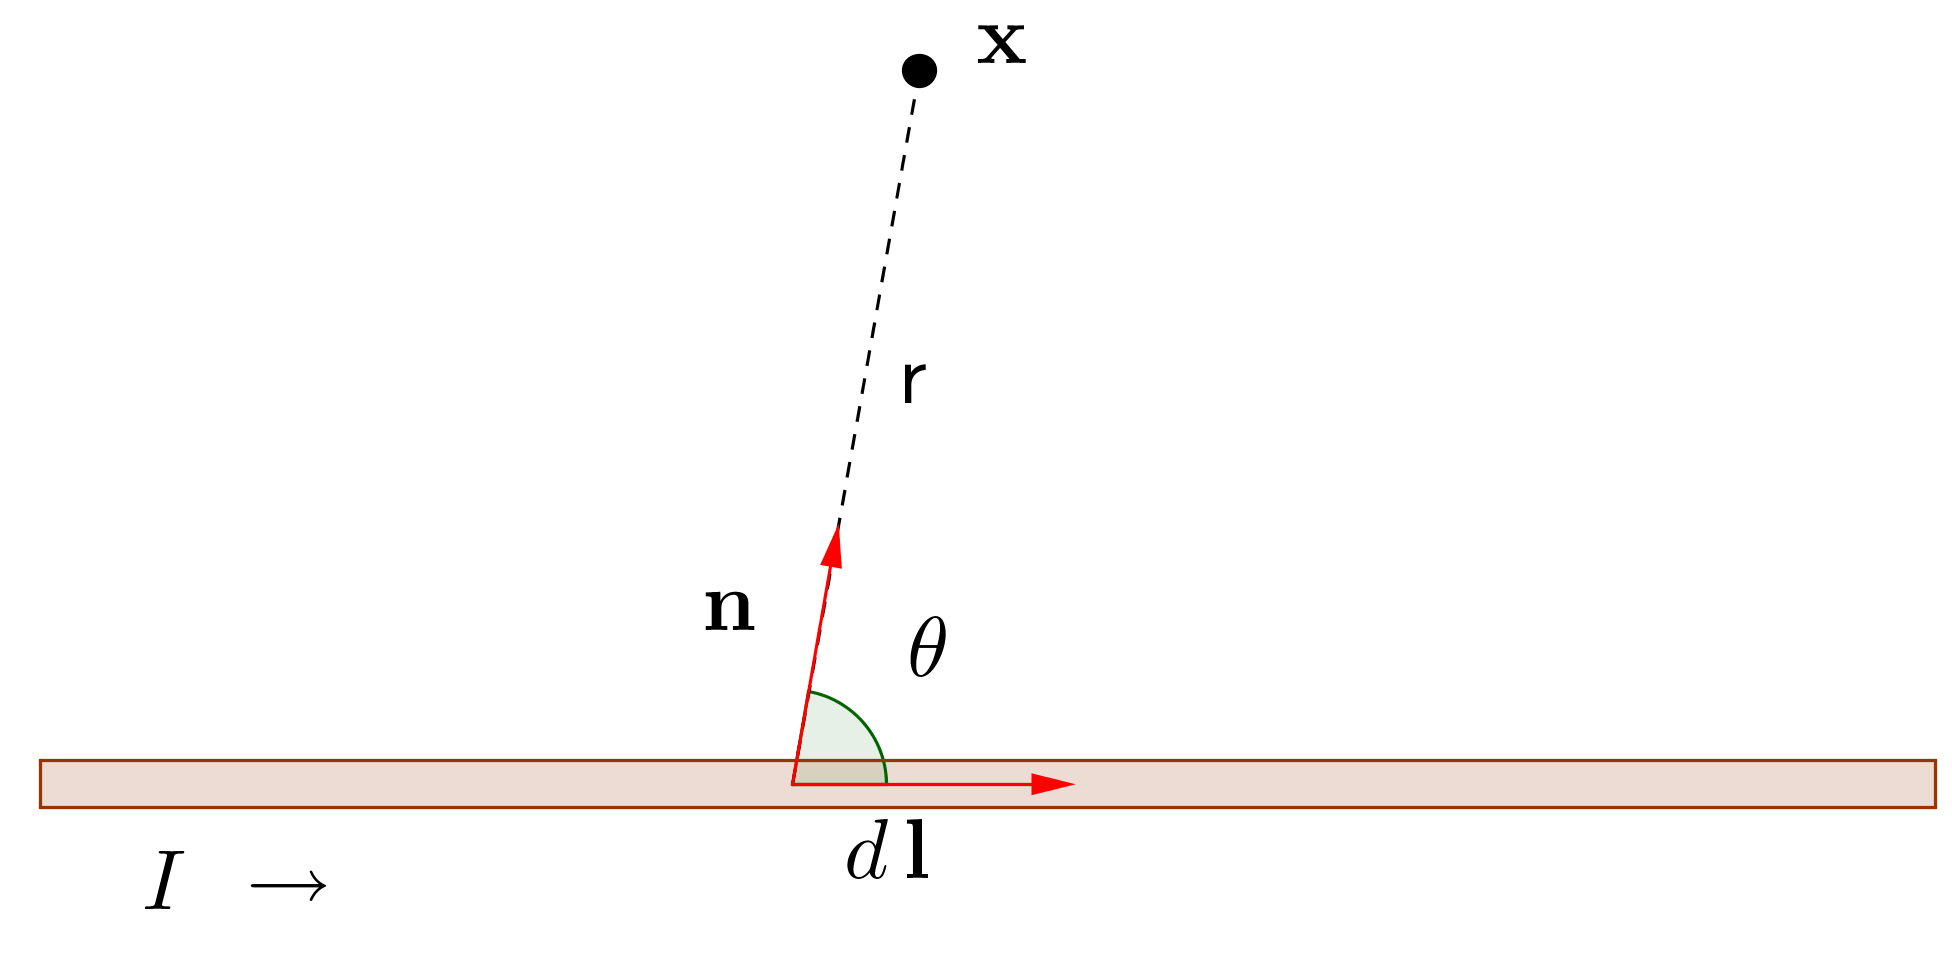
\includegraphics[scale=1.1]{corrente_fio}
\caption{\textit{Campo magnético no ponto $\textbf{x}$ devido a passagem de uma corrente elétrica $I$ pelo fio. Observe que a magnitude do campo depende também do ângulo $\theta$ entre $\textbf{l}$ e $\textbf{n}$}.}
\label{fig.corrente_fio}
\end{figure}
Assim sendo, a \textit{Lei de Biot-Savart} tem definição análoga à lei de Coulomb e pode ser expressa como
\begin{equation}\label{eq.lei_biot_savart}
d\,\textbf{B}=\frac{\mu_0\,I}{4\,\pi}\frac{d(\textbf{l}\times\textbf{n})}{r^2},
\end{equation}
e o campo magnético no volume ao redor do fio pode ser obtido integrando sobre a direção perpendicular ao plano formado por $\textbf{l}$ e $\textbf{n}$ ao longo do comprimento do fio.
\begin{equation}
\textbf{B}=\frac{\mu_0I}{4\,\pi}\int_{\textbf{l}}\frac{d(\textbf{l}\times\textbf{n})}{r^2}.
\end{equation}

Considere agora um laço circular (linha de campo magnético) de raio $r$ contido num plano perpendicular ao fio condutor, divido em pequenos comprimentos $\Delta\textbf{s}=\Delta s\,\pmb{\phi}$, cujos vetores correspondentes apontam na direção do vetor tangencial à circunferência naquele ponto, conforme  a figura tal. Esse laço fechado contido num plano é denominado \textit{laço Amperiano} e é usado para calcular o campo magnético referente àquela linha de campo tomando o limite quando $\Delta\textbf{s}\to 0$ e integrando no intervalo dado pelo comprimento da circunferência. Repare, pela figura \ref{fig.corrente_fio}, que nesse caso $\theta=\pi rd$ e que $\pmb{\phi}$ é perpendicular ao plano formado por $\textbf{l}$ e $\textbf{n}$, portanto a magnitute do vetor  $\textbf{B}$ na direção $\pmb{\phi}$ é dada pela lei de Biot-Savart na equação \ref{eq.lei_biot_savart}.
\begin{equation*}
\int_{s}\textbf{B}\cdot d\textbf{s}=B\int_{s}ds=\frac{\mu_0I}{2\pi\,r}2\pi\,r=\mu_0I.
\end{equation*} 
\begin{figure}[h]
\centering
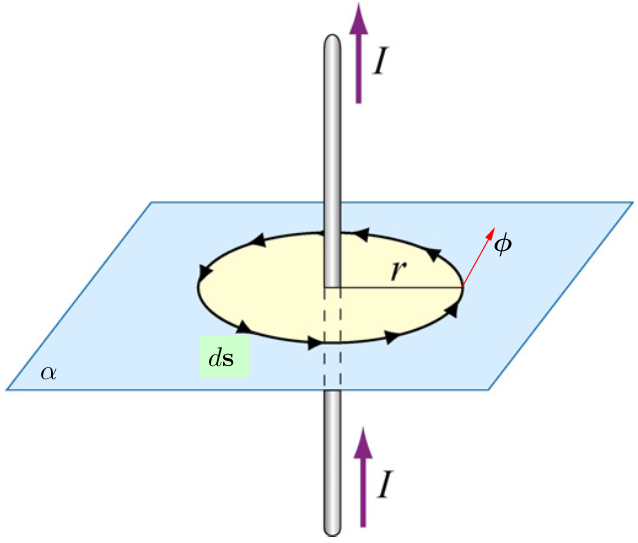
\includegraphics[scale=.5]{laco_amperiano}
\caption{\textit{Laço amperiano seguindo a regra da mão direita: posicionando o polegar no sentido da corrente, o campo magnético tem o mesmo sentido dos demais dedos curvando em torno do fio.}}
\label{fig.laco_amperiano}
\end{figure}

Vamos considerar um outro exemplo de laço amperiano cujo contorno denotado por $abcda$ se sobrepõe a duas linhas de campo magnético coplanares, observado na figura tal. No desenvolvimento abaixo, a primeira e terceira integrais zeram pois o campo magnético é perpendicular ao caminho de integração nesses intervalos, e $B_2(r_2\theta)$ e $B_1[r_1(2\pi-\theta)]$ são os comprimentos dos arcos $bc$ e $da$, respectivamente. A integral de linha do campo magnético no contorno $abcda$ é
\begin{align*}
\int_{abcda}\textbf{B}\cdot d\textbf{s}&=\int_{ab}\textbf{B}\cdot d\textbf{s}+\int_{bc}\textbf{B}\cdot d\textbf{s}+\int_{cd}\textbf{B}\cdot d\textbf{s}=\int_{da}\textbf{B}\cdot d\textbf{s}\\
&=0+B_2(r_2\theta)+0+B_1[r_1(2\pi-\theta)]\\
&=\frac{\mu_0I}{2\pi\,r_2}(r_2\theta)+\frac{\mu_0I}{2\pi\,r_1}[r_1(2\pi-\theta)]\\
&=\frac{\mu_0I}{2\pi}\theta+\frac{\mu_0I}{2\pi}(2\pi-\theta)\\
&=\mu_0I.
\end{align*}
\begin{figure}
\centering
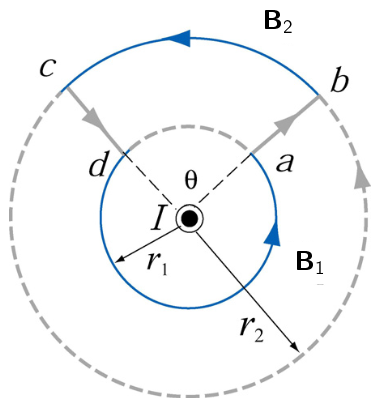
\includegraphics[scale=.5]{laco_amperiano_2}
\caption{\textit{Laço amperiano passando por duas linhas de campo. O ponto no centro significa que o sentido da corrente elétrica está ``saindo do plano do papel".}}
\label{fig.laco_amper_2}
\end{figure}
Vemos o mesmo resultado se o laço amperiano envolve uma ou duas linhas de campo magnético e, usando coordenadas cilíndricas, podemos demonstrar que o mesmo resultado é válido para uma quantidade arbitrária de linhas de campo magnético, ou seja, a integral de linha do campo magnético através de qualquer laço amperiano fechado é proporcional à corrente elétrica inscrita no laço. A \textit{Lei de Ampère} é dada por
\begin{equation*}
\int_{s}\textbf{B}\cdot d\textbf{s}=\mu_0I.
\end{equation*}
Analogamente à lei de Gauss para campos elétricos, para ser aplicada a lei de Ampère é necessário que o laço possua alguma simetria em relação ao fio. No caso de um fio condutor suficientemente grande para que suas extremidades não interfiram na aplicação, temos uma simetria cilíndrica e a lei de Ampère pode ser aplicada normalmente. Caso contrário, devemos utilizar a lei de Biot-Savart. 

Agora considere a seguinte situação, descrita por Maxwell, onde o circuito elétrico está interrompido por um capacitor. 
\begin{figure}
\centering
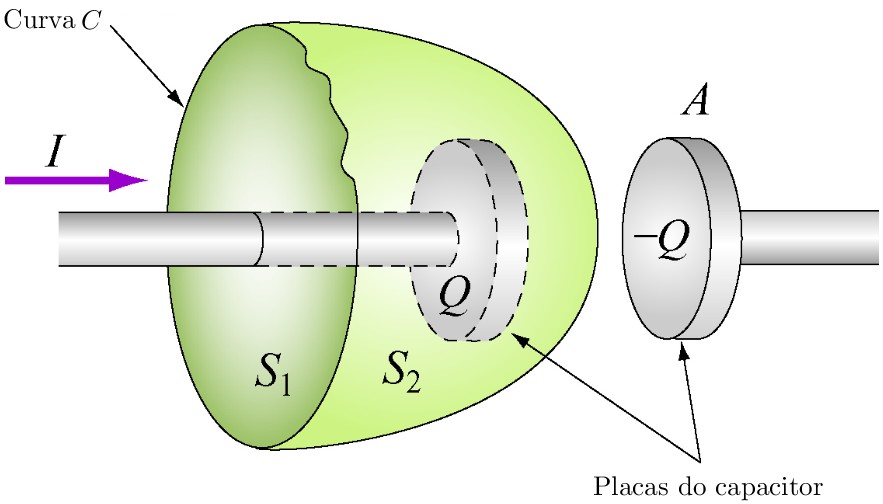
\includegraphics[scale=.3]{capacitor}
\caption{\textit{Quando há corrente no circuito, cargas positivas se acumulam numa placa do capacitor assim como cargas negativas se acumulam na outra placa. Tal acúmulo gera um fluxo elétrico variável entre as placas.}}
\label{fig.capacitor}
\end{figure}
Como vimos pela lei de Ampère, o campo magnético depende somente da corrente no circuito e do comprimento da circunferência que limita a superfície atravessada pelo fio condutor, e não depende dessa superfície em si. Portanto, o campo magnético referente à curva $C$ da figura \ref{fig.capacitor} pode ser calculado considerando a superfície $S_1$ ou a superfície $S_2$. A superfície $S_1$ é atravessada pela corrente $I$ a qual produz o campo magnético $\mathbf{B}$, mas superfície $S_2$ não é atravessada por $I$ e, no entanto, é produzido o mesmo campo magnético $\mathbf{B}$. Assim podemos sugerir que exista um outro fenômeno físico entre as placas do capacitor que seja responsável pela geração de $\mathbf{B}$. À medida que o capacitor vai sendo carregado, cargas elétricas opostas vão se acumulando em sua placas gerando um campo elétrico variável entre as placas, o qual produz um fluxo elétrico variável através da área da placa do capacitor. Maxwell mostrou que que o produto da variação desse fluxo elétrico pela permissividade elétrica no vácuo era numericamente igual à corrente $I$, e por isso produzia o mesmo campo $\mathbf{B}$ quando integrado longo da curva $C$,
\begin{equation*}
I_d=\epsilon_0\frac{d\phi_E}{dt}.
\end{equation*}
Tal produto foi denominado \textit{corrente deslocada} e foi adicionado à lei de Ampère, a qual se tornou a \textit{lei de Ampére generalizada} ou \textit{lei de Ampère-Maxwell},
\begin{equation*}
\int_s\mathbf{B}\cdot d\mathbf{s}=\mu_0I+\mu_0\epsilon_0\frac{d\phi_E}{dt}.
\end{equation*}
Note que quando consideramos a superfície $S_1$, $I_d=0$ já que o fluxo elétrico é constante e assim $\mathbf{B}$ é dado somente por $I$. Quando consideramos a superfície $S_2$, $I=0$ e $\mathbf{B}$ é dado somente por $I_d$. 




\subsection{A Lei de Faraday}
Analogamente ao caso da força gravitacional, o \textit{trabalho} $W$ realizado por uma força elétrica $\textbf{F}_e$ para levar uma carga elétrica $q$ de um ponto $A$ até um ponto $B$ é definido como
\begin{equation}\label{eq.trabalho}
W=\int_{A}^{B}\textbf{F}_e\cdot d\textbf{s}.
\end{equation}
A diferença entre a \textit{energia potencial} $U$ em cada um dos pontos $A$ e $B$ é o que ocasiona o deslocamento da carga, assim a variação da energia potencial tem definição
\begin{equation}\label{eq.energia_potencial}
\Delta U=U_b-U_a=-\int_{A}^{B}\textbf{F}_e\cdot d\textbf{s}=-W.
\end{equation}
A \textit{diferença de potencial elétrico}, $\Delta V$, também chamada \textit{ddp}, é variação da energia potencial por unidade de carga elétrica $q$. Utilizando a equação \ref{eq.camp_elet}, que relaciona força elétrica e campo elétrico, podemos definir a ddp como
\begin{equation}\label{eq.ddp}
\Delta V=-\int_{A}^{B}\frac{\textbf{F}_e}{q}\cdot d\textbf{s}=-\int_{A}^{B}\textbf{E}\cdot d\textbf{s}
\end{equation}
A ddp representa a quantidade de trabalho por unidade de carga para mover a carga do ponto $A$ ao ponto $B$ e sua unidade de medida no SI é o volt ($V=\frac{J}{C}$). Observe nas definições acima que só importa os valores no pontos $A$ e $B$, e não importa necessariamente o caminho que a carga vai percorrer de um ponto até o outro. 

Agora, num circuito elétrico fechado, as cargas percorrem um determinado caminho a partir de uma fonte de energia elétrica. Essa fonte é chamada de \textit{força eletromotriz}, representada por $\varepsilon$, e que pode ser pensada como uma ``bomba" de cargas que as impulsiona de um potencial menor para um potencial maior. A força eletromotriz é definida como o trabalho realizado para mover uma carga unitária na direção de maior potencial, matematicamente,
\begin{equation*}
\varepsilon=\frac{dW}{dq}, 
\end{equation*}
também medida em volt. Como o campo magnético não produz trabalho, o trabalho realizado sobre o movimento das cargas deve ser devido a um campo elétrico e para escrever a força eletromotriz em termos do campo elétrico de forma análoga ao que foi feito nas equações \ref{eq.trabalho}, \ref{eq.energia_potencial} e \ref{eq.ddp}, devemos utilizar uma integral de linha, pois nesse caso a corrente percorre um determinado caminho. Como o campo elétrico é não-conservativo (senão não haveria corrente) o valor da integral é diferente de zero. Assim,
\begin{equation}\label{eq.emf_E_nc}
\varepsilon=\int_{linha}\pmb{E}\cdot d\pmb{s}.
\end{equation}
 
O \textit{fluxo magnético} é definido de maneira similar ao fluxo elétrico e o entendimento pode ser acompanhado pela figura \ref{fig.flux_ele}. O fluxo magnético através de uma superfície é definido como
\begin{equation*}
\phi_B=\textbf{B}\textbf{A}=B\,A\,\cos\theta,
\end{equation*}
onde o vetor área é $\textbf{A}=A\textbf{n}$, $\textbf{n}$ é o vetor normal à superfície atravessada, $A$ é a magnitude da área, $B=\textbf{B}\cdot\textbf{n}$ é a componente do campo magnético na direção do vetor normal e $\theta$ é o ângulo entre $\textbf{B}$ e $\pmb{A}$. Tomando um elemento infinitesimal da área e integrando sobre a superfície o fluxo magnético é
\begin{equation*}
\phi_B=\int\int_S\pmb{B}\,d\pmb{A},
\end{equation*}
medido em \textit{Weber}, $Wb=\frac{T}{m^2}$. 

Em 1831, Faraday descobriu que se pode criar um campo elétrico variando um campo magnético em função do tempo num fenômeno que foi batizado de \textit{indução eletromagnética}. Um dos experimentos de Faraday (figura tal) consiste em movimentar um ímã dentro de uma bobina feita de fio condutor onde se pode observar a geração de uma corrente elétrica, como se a bobina estivesse conectada a fonte de força eletromotriz. O experimento mostra que a força eletromotriz induzida é proporcional à taxa (negativa) de variação do fluxo magnético através da bobina, a \textit{lei de Faraday} é
\begin{equation*}
\varepsilon=-\frac{d\phi_B}{dt}.
\end{equation*}
Podemos reescrever a lei de Faraday usando a equação \ref{eq.emf_E_nc},
\begin{equation*}
\varepsilon=\int_{linha}\pmb{E}\cdot d\pmb{s}=-\frac{d\phi_B}{dt},
\end{equation*}
o que implica que a variação do fluxo magnético induz um campo elétrico não-conservativo que varia com o tempo, diferente do campo elétrico conservativo gerado por cargas elétricas estacionárias.

%\begin{figure}[!htb]
%\centering
%\includegraphics[scale=5]{•}
%\caption{\textit{•}}
%\label{fig.exper_faraday}
%\end{figure}









\section{Equações de Maxwell}

\section{Generalizações da teoria}

\section{Conclusões}
%\chapter{Fundamentos de Elasticidade}\label{sec.fund_elast}

\section{Introdu\c{c}\~ao}
A teoria formal da propaga\c{c}\~ao de ondas s\'ismicas repousa nas intera\c{c}\~oes entre as part\'iculas infinitesimais discretas do meio \`a medida que uma deforma\c{c}\~ao se propaga. \'E muito dif\'icil estudar individualmente cada uma dessas intera\c{c}\~oes, mas dados experimentais que foram coletados como resultados dessas intera\c{c}\~oes sugerem que as mesmas podem ser consideradas em conjunto. Assim, o estudo da propaga\c{c}\~ao de ondas s\'ismicas atrav\'es de camadas de subsuperf\'icie num material discretizado pode ser feito considerando o meio como cont\'inuo, e tais estudos s\~ao os objetos da \textit{mec\^anica do cont\'inuo}. 

No desenvolvimento te\'orico da mec\^anica do cont\'inuo n\~ao s\~ao consideradas as caracter\'isticas at\^omicas da mat\'eria bem como as intera\c{c}\~oes entre essas part\'iculas, ou seja, a mat\'eria n\~ao \'e estudada do ponto de vista microsc\'opico. Segundo \cite{slawinski}, tal abordagem se justifica pelo fato de que a mat\'eria \'e formada por part\'iculas suficientemente pouco espa\c{c}adas e suas caracter\'isticas e comportamento podem ser descritos por fun\c{c}\~oes cont\'inuas e diferenci\'aveis. Assim, \'e assummido que elementos infinitesimais da mat\'eria t\^em as mesmas propriedades observadas em experimentos macrosc\'opicos, pois essa hip\'otese permite a cria\c{c}\~ao de um modelo matem\'atico abstrato \textit{efetivo} na descri\c{c}\~ao da realidade f\'isica. Como exemplo, vamos considerar a cor de um objeto. Pr\'otons e el\'etrons n\~ao possuem cor, mas os meios materiais (que s\~ao formados por pr\'otons e el\'etrons) t\^em a capacidade de absorver ou refletir determinados comprimentos de ondas eletromagn\'eticas as quais determinam a cor de cada meio. Outros conceitos da mec\^anica do cont\'inuo s\~ao elasticidade, viscosidade, fric\c{c}\~ao, rigidez, etc, como veremos mais a frente.


\section{Fatos experimentais}
A teoria sobre elasticidade est\'a baseada em conceitos primitivos e conclus\~oes estabelecidas a partir de fatos experimentais verificados em v\'arios textos sobre o assunto como \cite{liu}, \cite{dahlem} e \cite{slawinski}. Adicionalmente, em geral as equa\c{c}\~oes que governam a propaga\c{c}\~ao de ondas em meios el\'asticos s\~ao n\~ao-lineares. Contudo, em experimentos s\'ismicos foi constatado que aspectos importantes da propaga\c{c}\~ao de ondas podem ser analisados a partir de equa\c{c}\~oes lineares, resultando numa abordagem chamada \textit{teoria da elasticidade linearizada}.

\subsection{Deforma\c{c}\~ao}

A \textit{deforma\c{c}\~ao} de um meio el\'astico cont\'inuo \'e a mudan\c{c}a na posi\c{c}\~ao dos pontos que comp\~oem o corpo em rela\c{c}\~ao uns aos outros. Ou seja, h\'a uma mudan\c{c}a relativa entre os pontos e n\~ao um deslocamento do corpo como um todo e sem mudan\c{c}a de sua forma, caso em que ter\'iamos um \textit{movimento r\'igido}. Nesta subse\c{c}\~ao estamos interessados nas caracter\'isticas geom\'etricas relativas \`a deforma\c{c}\~ao de um corpo. N\~ao estamos considerando as causas de deforma\c{c}\~ao de um corpo, como aplica\c{c}\~ao de carga ou varia\c{c}\~ao de temperatura, nem discutiremos a composi\c{c}\~ao do material, assumindo apenas que o mesmo seja cont\'inuo e el\'astico. Assim, vamos relacionar as caracter\'isticas geom\'etricas de um corpo antes da deforma\c{c}\~ao com as caracter\'isticas ap\'os a deforma\c{c}\~ao.

\subsection{Dedu\c{c}\~ao do Tensor de Deforma\c{c}\~oes}\label{sec.deriva_deforma}

Para determinar o tensor de deforma\c{c}\~oes vamos considerar dois pontos pertencentes ao espaco $\mathbb{R}^3$ bastante pr\'oximos um do outro denotados por
\begin{align*}
\mathbf{x}&=(x_1,x_2,x_3)\quad\text{e}\\
\mathbf{y}=\mathbf{x}+d\mathbf{s}&=(x_1+dx_1,x_2+dx_2,x_3+dx_3),
\end{align*}
e que podem ser observados na figura \ref{fig.deformacao_meio}. O quadrado da dist\^ancia entre esses dois pontos \'e
\begin{equation}\label{eq.dist_antes_defor}
\norm{d\mathbf{s}}^2=(dx_1)^2+(dx_2)^2+(dx_3)^2.
\end{equation}
\begin{figure}
\centering
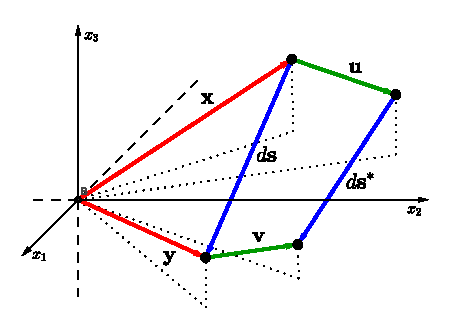
\includegraphics[scale=1.4]{deformacao_meio}
\caption{\textit{Mudan\c{c}a na posi\c{c}\~ao relativa entre os pontos que comp\~oem um  meio el\'astico cont\'inuo.}}
\label{fig.deformacao_meio}
\end{figure}
A aplica\c{c}\~ao de uma deforma\c{c}\~ao depende do ponto de aplica\c{c}\~ao, ou seja, a deforma\c{c}\~ao aplicada no ponto $\mathbf{x}$ difere da aplica\c{c}\~ao no ponto $\mathbf{y}$. Caso o vetor que d\'a a deforma\c{c}\~ao tenha componentes constantes, n\~ao teremos uma deforma\c{c}\~ao relativa, apenas uma transla\c{c}\~ao dos pontos. Assim, podemos definir o \textit{vetor de deslocamento} para cada ponto de aplica\c{c}\~ao
\begin{align*}
\mathbf{u}(\mathbf{x})&=(u_1,u_2,u_3),\\
\mathbf{v}(\mathbf{y})&=(v_1,v_2,v_3),
\end{align*}
e som\'a-los aos respectivos pontos $\mathbf{x}$ e $\mathbf{y}$ para obter suas posi\c{c}\~oes ap\'os a deforma\c{c}\~ao,
\begin{align*}
\mathbf{x}^*&=(x_1+u_1,x_2+u_2,x_3+u_3)\\
\mathbf{y}^*&=(x_1+dx_1+v_1,x_2+dx_2+v_2,x_3+dx_3+v_3).
\end{align*}
Subtraindo, obtemos o vetor que d\'a a diferen\c{c}a entre os pontos ap\'os a deforma\c{c}\~ao
\begin{equation}\label{eq.dist_apos_defor}
d\mathbf{s}^*=(dx_1+v_1-u_1,dx_2+v_2-u_2,dx_3+v_3-u_3).
\end{equation}
Como a varia\c{c}\~ao entre os pontos $\mathbf{x}$ e $\mathbf{y}$ \'e infinitesimal, vamos aplicar a expans\~ao de Taylor de segunda ordem em torno do ponto $\mathbf{x}$ e desprezar o resto de Lagrange para escrever as componentes de $\mathbf{v}$ em fun\c{c}\~ao das componentes de $\mathbf{u}$, aproximadamente,
\begin{align*}
v_1&\approx u_1+\frac{\partial u_1}{\partial x_1}\Bigg\vert_{\mathbf{x}}dx_1+\frac{\partial u_1}{\partial x_2}\Bigg\vert_{\mathbf{x}}dx_2+\frac{\partial u_1}{\partial x_3}\Bigg\vert_{\mathbf{x}}dx_3\\\\
v_2&\approx u_2+\frac{\partial u_2}{\partial x_1}\Bigg\vert_{\mathbf{x}}dx_1+\frac{\partial u_2}{\partial x_2}\Bigg\vert_{\mathbf{x}}dx_2+\frac{\partial u_2}{\partial x_3}\Bigg\vert_{\mathbf{x}}dx_3\\\\
v_3&\approx u_3+\frac{\partial u_3}{\partial x_1}\Bigg\vert_{\mathbf{x}}dx_1+\frac{\partial u_3}{\partial x_2}\Bigg\vert_{\mathbf{x}}dx_2+\frac{\partial u_3}{\partial x_3}\Bigg\vert_{\mathbf{x}}dx_3.
\end{align*}
Substituindo esses valores na equa\c{c}\~ao \ref{eq.dist_apos_defor}, simplificando e introduzindo a nota\c{c}\~ao de somat\'orio temos
\begin{equation*}
d\mathbf{s}^*\approx\left(dx_1+\sum_{i=1}^3\frac{\partial u_1}{\partial x_i}\Bigg\vert_{\mathbf{x}}dx_i\,,\,dx_2+\sum_{i=1}^3\frac{\partial u_2}{\partial x_i}\Bigg\vert_{\mathbf{x}}dx_i\,,\,dx_3+\sum_{i=1}^3\frac{\partial u_3}{\partial x_i}\Bigg\vert_{\mathbf{x}}dx_i\right).
\end{equation*}
O quadrado da dist\^ancia entre os pontos ap\'os a deforma\c{c}\~ao \'e dado por
\begin{equation*}
\norm{d\mathbf{s}^*}^2\approx\left(dx_1+\sum_{i=1}^3\frac{\partial u_1}{\partial x_i}\Bigg\vert_{\mathbf{x}}dx_i\right)^2+\left(dx_2+\sum_{i=1}^3\frac{\partial u_2}{\partial x_i}\Bigg\vert_{\mathbf{x}}dx_i\right)^2+\left(dx_3+\sum_{i=1}^3\frac{\partial u_3}{\partial x_i}\Bigg\vert_{\mathbf{x}}dx_i\right)^2.
\end{equation*}
Abrindo cada uma das parcelas quadr\'aticas, temos
\begin{align*}
\norm{d\mathbf{s}^*}^2&\approx(dx_1)^2+2\,dx_1\,\sum_{i=1}^3\frac{\partial u_1}{\partial x_i}\Bigg\vert_{\mathbf{x}}dx_i+\left(\sum_{i=1}^3\frac{\partial u_1}{\partial x_i}\Bigg\vert_{\mathbf{x}}dx_i\right)^2\\\\
&+(dx_2)^2+2\,dx_2\,\sum_{i=1}^3\frac{\partial u_2}{\partial x_i}\Bigg\vert_{\mathbf{x}}dx_i+\left(\sum_{i=1}^3\frac{\partial u_2}{\partial x_i}\Bigg\vert_{\mathbf{x}}dx_i\right)^2\\\\
&+(dx_3)^2+2\,dx_3\,\sum_{i=1}^3\frac{\partial u_3}{\partial x_i}\Bigg\vert_{\mathbf{x}}dx_i+\left(\sum_{i=1}^3\frac{\partial u_3}{\partial x_i}\Bigg\vert_{\mathbf{x}}dx_i\right)^2.
\end{align*}
Pela equa\c{c}\~ao \ref{eq.dist_antes_defor}, a coluna  da esquerda \'e $\norm{d\mathbf{s}}^2$. Como estamos trabalhando com quantidades infinitesimais, podemos negligenciar a coluna da direita por se tratar do quadrado do gradiente de cada componente do vetor de deslocamento num produto escalar com o vetor que d\'a a dist\^ancia entre os pontos $\mathbf{x}$  e $\mathbf{y}$. A coluna do meio se desdobra em dezoito parcelas que podem ser reagrupadas num somat\'orio duplo. Assim,
\begin{equation*}
\norm{d\mathbf{s}^*}^2\approx\norm{d\mathbf{s}}^2+\sum_{i=1}^3\sum_{j=1}^3\left(\frac{\partial u_i}{\partial x_j}\Bigg\vert_{\mathbf{x}}+\frac{\partial u_j}{\partial x_i}\Bigg\vert_{\mathbf{x}}\right)dx_i\,dx_j,
\end{equation*}
onde o termo entre par\^enteses \'e definido como o \textit{tensor de deforma\c{c}\~ao} na teoria da elasticidade,
\begin{equation*}
\varepsilon_{i,j}=\frac{1}{2}\left(\frac{\partial u_i}{\partial x_j}\Bigg\vert_{\mathbf{x}}+\frac{\partial u_j}{\partial x_i}\Bigg\vert_{\mathbf{x}}\right),\qquad\text{e}\qquad i,j\,\in\,\{1,2,3\}.
\end{equation*}
Considerando deslocamentos infinitesimais, os componentes desse tensor nos permitem descrever as deforma\c{c}\~oes associadas a esses deslocamentos entre os pontos iniciais. Analisando as entradas do tensor vemos que se o vetor de deslocamento \'e constante ent\~ao $\epsilon_{i,j}=0$ para todo o tensor, e n\~ao h\'a deforma\c{c}\~ao, apenas movimento r\'igido como descrito anteriormente. Como se trata de uma matriz sim\'etrica, no espa\c{c}o $\mathbb{R}^3$ temos apenas seis componentes independentes para o tensor.

\subsection{Interpreta\c{c}\~ao Geom\'etrica do Tensor de Deforma\c{c}\~ao}

Existem basicamente dois tipos de deforma\c{c}\~oes descritas pelo tensor, uma onde podemos ter mudan\c{c}a de comprimento em alguma dimens\~ao ocasionando mudan\c{c}a de volume, mas sem mudan\c{c}a na forma do corpo estudado. Outra com mudan\c{c}a na forma mas sem mudan\c{c}a de volume. Vamos analisar como cada entrada do tensor \'e respons\'avel por altera\c{c}\~oes geom\'etricas do meio.

\subsubsection{Altera\c{c}\~ao Relativa de Comprimento}\label{sec.alte_compri}

Considerando o caso unidimensional, vamos aplicar as deforma\c{c}\~oes $\mathbf{u}$ e $\mathbf{v}$ aos pontos $\mathbf{x}=(x_1,0,0)$ e $\mathbf{y}=(x_1+dx_1,0,0)$, respectivamente,
\begin{equation*}
\mathbf{x}^*=(x_1+u_1,u_2,u_3)\quad\text{e}\quad\mathbf{y}^*=(x_1+dx_1+v_1,v_2,v_3).
\end{equation*}
Calculando a dist\^ancia entre os pontos ap\'os a deforma\c{c}\~ao temos
\begin{equation*}
d\mathbf{s}^*=(dx_1+v_1-u_1,v_2-u_2,v_3-u_3).
\end{equation*}
Analogamente a subse\c{c}\~ao \ref{sec.deriva_deforma}, vamos usar a expans\~ao de Taylor e ignorar o resto de Lagrange para escrever a primeira componente de $\mathbf{v}$ em fun\c{c}\~ao da primeira componente de $\mathbf{u}$. 
\begin{equation*}
v_1(\mathbf{y})=u_1(\mathbf{x})+\frac{\partial u_1}{\partial x_1}\Bigg\vert_{\mathbf{x}}dx_1+\frac{1}{2}\frac{\partial^2 u_1}{\partial x_1^2}\Bigg\vert_{\mathbf{x}}(dx_1)^2+\cdots
\end{equation*}
Novamente, utilizando a aproxima\c{c}\~ao para os dois primeiros termos e substituindo a primeira componente do vetor $d\mathbf{s}^*$, temos
\begin{equation}
dx_1^*\approx dx_1+\frac{\partial u_1}{\partial x_1}\Bigg\vert_{\mathbf{x}}dx_1\approx \left(1+\frac{\partial u_1}{\partial x_1}\Bigg\vert_{\mathbf{x}}\right)\,dx_1. 
\end{equation}
Usando a nota\c{c}\~ao dos componentes do tensor de deforma\c{c}\~ao, temos
\begin{equation}\label{eq.defor_unidi}
dx_1^*\approx(1+\epsilon_{11})\,dx_1.
\end{equation} 
Assim, vemos que $\epsilon_{11}$ \'e uma contra\c{c}\~ao ou dilata\c{c}\~ao ao longo do eixo $x_1$ e, analogamente, podemos demonstrar que $\epsilon_{22}$ e $\epsilon_{33}$ determinam a distens\~ao ou contra\c{c}\~ao ao longo dos eixos $x_2$ e $x_3$, respectivamente.
Utilizando um abuso de nota\c{c}\~ao, podemos escrever a express\~ao \ref{eq.defor_unidi} como
\begin{equation*}
\frac{dx_1^*}{dx_1}\approx \frac{\partial x_1+\partial u_1}{\partial x_1},
\end{equation*}
e desse jeito podemos perceber que o fator $(1+\epsilon_{11})$ \'e uma mudan\c{c}a relativa (citada na subse\c{c}\~ao \ref{sec.deriva_deforma}) no comprimento ao longo do eixo $x_1$ devido a deforma\c{c}\~ao.

\subsubsection{Altera\c{c}\~ao Relativa de Volume}

Para estudar as altera\c{c}\~oes no volume de um s\'olido el\'astico vamos considerar uma caixa retangular (paralelep\'ipedo) com dimens\~oes $\Delta x_1, \Delta x_2\,\text{e}\,\Delta x_3$ nas dire\c{c}\~oes dos eixos coordenados.  Dessa forma, o volume do paralelep\'ipedo \'e dado por\begin{equation*}
V=\Delta x_1\,\Delta x_2\,\Delta x_3.
\end{equation*}
Conforme subse\c{c}\~ao \ref{sec.alte_compri}, aplicando a mudan\c{c}a relativa de comprimento a cada uma das tr\^es dimans\~oes, temos que ap\'os a deforma\c{c}\~ao, o volume do s\'olido \'e dado por
\begin{align}\nonumber
V^*&=(1+\epsilon_{11})\Delta x_1\,(1+\epsilon_{22})\Delta x_2\,(1+\epsilon_{33})\Delta x_3\\\label{eq.altera_volume}
&=(1+\epsilon_{11})\,(1+\epsilon_{22})\,(1+\epsilon_{33})\,V.
\end{align}
Como a deforma\c{c}\~ao aplicada tem tamanho infinitesimal, estamos supondo que as altera\c{c}\~oes relativas de comprimento n\~ao fujam significativamente das dire\c{c}\~oes can\^onicas dos eixos coordenados, assim h\'a altera\c{c}\~ao apenas no volume do s\'olido e n\~ao no seu formato. Ainda por conta do valores infinitesimais de $\epsilon_{ii}$, podemos negligenciar os termos n\~ao lineares resultantes da multiplica\c{c}\~ao na equa\c{c}\~ao \ref{eq.altera_volume} e aproximar o volume ap\'os a deforma\c{c}\~ao para
\begin{equation}\label{eq.altera_volume_2}
V^*\approx(1+\epsilon_{11}+\epsilon_{22}+\epsilon_{33})\,V.
\end{equation}
Observe que $\epsilon_{11}+\epsilon_{22}+\epsilon_{33}$ \'e o tra\c{c}o do tensor de deforma\c{c}\~ao, pode ser calculado atrav\'es do divergente do vetor de deslocamento e ser\'a denotado por $\varphi$ definindo a \textit{dilata\c{c}\~ao},
\begin{align*}
\varphi &=\epsilon_{11}+\epsilon_{22}+\epsilon_{33}\\
&=\frac{\partial u_1}{\partial x_1}+\frac{\partial u_2}{\partial x_2}+\frac{\partial u_3}{\partial x_3}\\
&=\left(\frac{\partial}{\partial x_1},\frac{\partial}{\partial x_2},\frac{\partial}{\partial x_3}\right)\cdot(u_1,u_2,u_3)\\
&=\nabla\cdot \mathbf{u}.
\end{align*}
Como o tra\c{c}o de uma matriz \'e um escalar e este n\~ao se altera quando \'e aplicada uma transforma\c{c}\~ao nos eixos coordenados, temos que a dilata\c{c}\~ao e a consequente altera\c{c}\~ao no volume de um s\'olido n\~ao depende do sistema de coordenadas escolhido. Manipulando a equa\c{c}\~ao \ref{eq.altera_volume_2} podemos constatar que a dilata\c{c}\~ao se trata de uma mudan\c{c}a relativa do volume
\begin{equation*}
\frac{V^*-V}{V}\approx\epsilon_{11}+\epsilon_{22}+\epsilon_{33}.
\end{equation*}

\subsubsection{Altera\c{c}\~ao Relativa na Forma}

O tensor de deforma\c{c}\~ao tamb\'em descreve uma mudan\c{c}a no formato do corpo, conforme podemos acompanhar pela figura \ref{fig.deforma_formato}, onde um ret\^angulo \'e transformado num paralelogramo. 
\begin{figure}
\centering
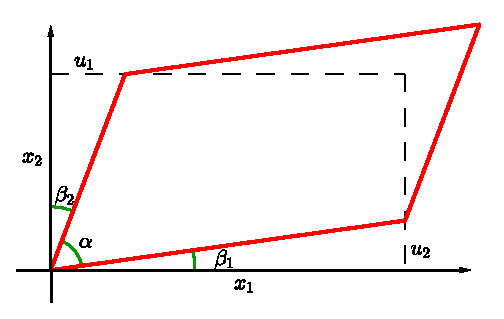
\includegraphics[scale=1.4]{deforma_formato}
\caption{\textit{Exemplo em duas dimens\~oes de como algumas componentes do tensor de deforma\c{c}\~ao promove a varia\c{c}\~ao no formato do meio.}}
\label{fig.deforma_formato}
\end{figure}
O angulo reto inicialmente formado pelos eixos coordenados $x_1$ e $x_2$ \'e reduzido a um \^angulo $\alpha$ que obedece \`a rela\c{c}\~ao
\begin{equation*}
\alpha=\frac{\pi}{2}-\beta_1-\beta_2,
\end{equation*}
onde $\beta_1$ e $\beta_2$ s\~ao os \^angulos formados pelos lados do paralelogramo e os eixos $x_1$ e $x_2$, respectivamente. Como a varia\c{c}\~ao angular \'e bastante pequena, temos que cada \^angulo $\beta_i$ pode ser aproximado por sua respectiva tangente, e considerando deslocamentos infinitesimais, temos
\begin{align*}
\beta_1+\beta_2&\approx\tan(\beta_1)+\tan(\beta_2)\\
&=\frac{\partial u_2}{\partial x_1}+\frac{\partial u_1}{\partial x_2}\\
&=2\epsilon_{12}=2\epsilon_{21}.
\end{align*}
Portanto, temos que o tensor de deforma\c{c}\~ao tamb\'em \'e respons\'avel pela altera\c{c}\~ao na dire\c{c}\~ao dos seguimentos que comp\~oem um corpo, mudando assim seu formato.


\subsection{Conserva\c{c}\~ao da Massa, Tens\~ao e o Equil\'ibrio do Momento Linear}\label{sec.massa_tensao_momen_lin}

O princ\'ipio de conserva\c{c}\~ao da massa \'e fundamental em mec\^anica do cont\'inuo na determina\c{c}\~ao da rela\c{c}\~ao entre o vetor de deslocamento $\mathbf{u}$ e a densidade de massa de um corpo $\rho$. Por defini\c{c}\~ao, a quantidade de massa ocupando um volume $V$  num dado tempo $t$ \'e
\begin{equation*}
m=\iiint_V\rho\,dV,
\end{equation*}
onde tanto a massa como a densidade n\~ao dependem apenas do tempo mas tamb\'em da posi\c{c}\~ao $\mathbf{x}$. Fixado um volume $V$, a taxa de varia\c{c}\~ao da massa no tempo \'e dada por
\begin{equation}\label{eq.massa_1}
\frac{d}{dt}m=\iiint_V\frac{\partial\rho}{\partial t}dV.
\end{equation}
Assumindo que n\~ao h\'a destrui\c{c}\~ao nem produ\c{c}\~ao de massa dentro do volume, a varia\c{c}\~ao da massa se d\'a apenas pelo quantidade de massa que passa pelo volume, ou que passa atrav\'es de uma das superf\'icies que limita esse volume, o que pode ser escrito como
\begin{equation}\label{eq.massa_2}
\frac{dm}{dt}=-\iint_S\rho\,\mathbf{v}\cdot d\mathbf{S},
\end{equation}
onde $\mathbf{v}$ \'e a velocidade da quantidade de massa que atravessa a superf\'icie $S$. A superf\'icie infinitesimal $dS$ \'e pequena o suficiente para ser considerada plana e tem o mesmo fluxo de massa em todos os seus pontos, e o sinal negativo decorre do fato de que o vetor normal \`a superf\'icie aponta no sentido de sa\'ida do volume. 

Substituindo a equa\c{c}\~ao \ref{eq.massa_2} na equa\c{c}\~ao \ref{eq.massa_1} temos
\begin{equation}\label{eq.massa_3}
\iiint_V\frac{\partial\rho}{\partial t}dV=-\iint_S\rho\,\mathbf{v}\cdot d\mathbf{S},
\end{equation}
ou seja, a taxa de varia\c{c}\~ao da quantidade de massa num determinado volume \'e proporcional \`a taxa de varia\c{c}\~ao da quantidade de massa que atravessa a superf\'icie que limita esse volume. Pelo teorema do divergente temos que
\begin{equation}\label{eq.massa_divergente}
\iint_S\rho\,\mathbf{v}\cdot d\mathbf{S}=\iiint_V\nabla\cdot (\rho\,\mathbf{v})\,dV,
\end{equation}
onde substiutindo a equa\c{c}\~ao \ref{eq.massa_divergente} na equa\c{c}\~ao \ref{eq.massa_3} e agrupando os integrandos sob um mesmo volume, temos
\begin{equation*}
\iiint_V\left[\frac{\partial\rho}{\partial t}+\nabla\cdot (\rho\,\mathbf{v})\right]\,dV=0,
\end{equation*}
que \'e a equa\c{c}\~ao que descreve a \textit{conserva\c{c}\~ao de massa} num determinado volume $V$.

Em geral, as for\c{c}as agindo no interior de um meio continuo s\~ao as chamadas \textit{for\c{c}as de superf\'icie}, ou seja, quando um material \'e submetido ao contato de uma carga em sua superf\'ice, for\c{c}as internas se propagam no inteiror do material atrav\'es de outras superf\'icies imagin\'arias provocando a deforma\c{c}\~ao desse material. Assim, podemos definir a \textit{tens\~ao} como o conjunto dessas for\c{c}as de superf\'ice, fazendo com que tens\~ao e deforma\c{c}\~ao estejam diretamente relacionadas. Matematicamente, tens\~ao media \'e definida como a for\c{c}a por unidade de \'area
\begin{equation}\label{eq.tensao_media}
\mathbf{\overline{T}}=\frac{\Delta\mathbf{F}}{\Delta S},
\end{equation}
e segundo o princ\'ipio fundamental da mec\^anica do cont\'inuo estabelecido por Cauchy, existe o limite para o valor da tens\~ao quando $\Delta S\to 0$,
\begin{equation*}
\mathbf{T}^{\mathbf{n}}=\lim_{\Delta S\to 0}\frac{\Delta\mathbf{F}}{\Delta S}=\frac{d\mathbf{F}}{dS}.
\end{equation*}
O vetor $\mathbf{n}$ \'e normal a superf\'icie de aplica\c{c}\~ao da tens\~ao $\mathbf{T}^{\mathbf{n}}$ e \'e \'util para identificar que determinada tens\~ao se aplica a determinada superf\'icie.

Al\'em das for\c{c}as de superf\'icie temos tamb\'em as for\c{c}as de corpo que agem \`a dist\^ancia como a for\c{c}a gravitacional ou a for\c{c}a el\'etrica que agem sobre um corpo material ou sobre uma carga el\'etrica, respectivamente. Denotando tal for\c{c}a por $\mathbf{f}(\mathbf{x},t)$ temos que a for\c{c}a total atuando num corpo \'e
\begin{equation}\label{eq.forca_total}
\mathbf{F}_T=\iint_S\mathbf{T}\,dS+\iiint_V\mathbf{f}\,dV,
\end{equation}
onde $V$ \'e o volume enclausurado pela superf\'icie $S$. Usando a defini\c{c}\~ao de for\c{c}a dada pela segunda lei de Newton, podemos reescrever a equa\c{c}\~ao \ref{eq.forca_total} como
\begin{equation}\label{eq.forca_total_2}
\frac{d}{dt}\iiint_V\rho\frac{d\mathbf{u}}{dt}\,dV=\iint_S\mathbf{T}\,dS+\iiint_V\mathbf{f}\,dV,
\end{equation}
onde $\mathbf{u}$ \'e o vetor deslocamento. A equa\c{c}\~ao \ref{eq.forca_total_2} estabelece o equil\'ibrio do \textit{momento linear}, ou seja, a taxa de varia\c{c}\~ao do momento linear de uma part\'icula no meio cont\'inuo \'e igual ao somat\'orio de for\c{c}as externas agindo nessa part\'icula. Discretizando a \'ultima integral da equa\c{c}\~ao acima podemos escrever
\begin{equation*}
\frac{1}{2}\sum_{i=1}^n\sum_{j=1}^n(\mathbf{F}_{ji}+\mathbf{F}_{ij}),
\end{equation*}
onde $\mathbf{F}_{ji}$ \'e a for\c{c}a exercida na part\'icula $i$ devida \`a part\'icula $j$. Pela terceira lei de Newton, for\c{c}as entre part\'iculas tem mesma intensidade e dire\c{c}\~ao e sentidos opostos, assim, $\mathbf{F}_{ji}=-\mathbf{F}_{ij}$. Mais ainda, uma part\'icula n\~ao exerce uma for\c{c}a em si mesma, ent\~ao $\mathbf{F}_{ii}=0$. Portanto, a equa\c{c}\~ao \ref{eq.forca_total_2} se resume a
\begin{equation*}
\frac{d}{dt}\iiint_V\rho\frac{d\mathbf{u}}{dt}\,dV=\iint_S\mathbf{T}\,dS.
\end{equation*}
Somente for\c{c}as externas s\~ao respons\'aveis por altera\c{c}\~oes no momento linear.

\subsection{O Tensor de Tens\~oes}\label{sec.tensor_tensoes}

Para deriva\c{c}\~ao do tensor de tens\~oes vamos utilizar o argumento do tetraedro de Cauchy, estudando as for\c{c}as agindo no inteiror de um meio cont\'inuo em rela\c{c}\~ao a um plano imagin\'ario com orienta\c{c}\~ao arbitr\'aria. O tetraedro \'e limitado pelos $O(0,0,0)$, $X(x,0,0)$, $Y(0,y,0)$ e $Z(0,0,z)$, contendo faces ortogonais, $OYZ$, $XOZ$ e $XYO$ e a face obl\'iqua $XYZ$, conforme a figura \ref{fig.tetraedro}.
\begin{figure}
\centering
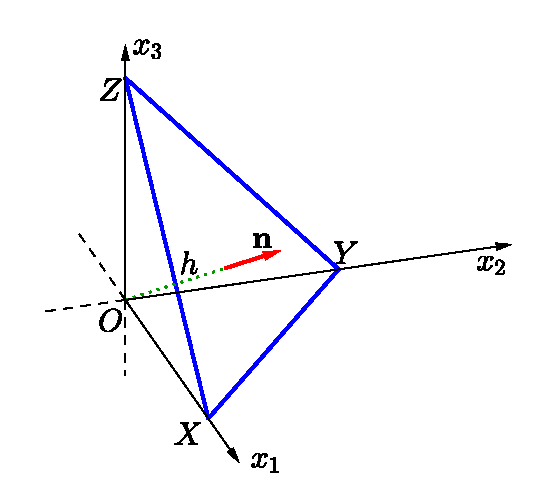
\includegraphics[scale=1]{tetraedro_cauchy}
\caption{\textit{Tetraedro de Cauchy, com for\c{c}as superficiais agindo em cada uma das faces ortogonais e na face obl\'iqua.}}
\label{fig.tetraedro}
\end{figure}

 Utilizando o equil\'ibro do momento linear dado pela equa\c{c}\~ao \ref{eq.forca_total_2}, podemos determinar a for\c{c}a agindo na face obl\'iqua de \'area $\Delta S$, considerando um tetraedro de dimens\~oes finitas.
\begin{equation}\label{eq.forca_total_3}
\overline{\rho}\,\Delta V\frac{d\overline{\mathbf{v}}}{dt}=\Delta \mathbf{F}+\Delta\mathbf{F}^{(\mathbf{e}_1)}+\Delta\mathbf{F}^{(\mathbf{e}_2)}+\Delta\mathbf{F}^{(\mathbf{e}_3)}+\overline{f}\Delta V,
\end{equation} 
onde $\Delta\mathbf{F}$ \'e a for\c{c}a superficial agindo na face obl\'iqua, $\Delta\mathbf{F}^{(\mathbf{e}_i)}$ \'e a for\c{c}a superficial agindo na face ortogonal cujo a normal \'e o eixo $x_i$, $\overline{f}$ \'e a for\c{c}a de campo agindo no tetraedro de volume $\Delta V$ e densidade $\rho$, e $\frac{d\overline{\mathbf{v}}}{dt}$ \'e a velocidade usada no c\'alculo da taxa de varia\c{c}\~ao do momento linear. As barras acima de cada s\'imbolo significam valores m\'edios para tetraedros de dimens\~oes finitas. Substituindo a equa\c{c}\~ao \ref{eq.tensao_media} na equa\c{c}\~ao \ref{eq.forca_total_3} temos
\begin{equation}\label{eq.forca_total_4}
\overline{\rho}\,\Delta V\frac{d\overline{\mathbf{v}}}{dt}=\mathbf{\overline{T}}^{(\mathbf{n})}\,\Delta S-\mathbf{\overline{T}}^{(\mathbf{e}_1)}\,\Delta S_1-\mathbf{\overline{T}}^{(\mathbf{e}_2)}\,\Delta S_2-\mathbf{\overline{T}}^{(\mathbf{e}_3)}\,\Delta S_3+\overline{f}\,\Delta V,
\end{equation}
onde $\Delta S_i$ \'e a \'area da face cujo a normal \'e o eixo $x_i$. Note, ainda pela figura \ref{fig.tetraedro}, que as faces ortogonais tem suas respectivas normais com a mesma dire\c{c}\~ao mas sentido oposto ao respectivo vetor unit\'ario $\mathbf{e}_i$ do eixo correspondente, da\'i o sinal negativo na equa\c{c}\~ao acima por conta da terceira lei de Newton. Para continuarmos nossa deriva\c{c}\~ao precisamos relacionar a \'area da face obl\'iqua com as \'areas das faces ortogonais. Observe que cada componente $n_i$ do vetor $\mathbf{n}$ \'e, por defini\c{c}\~ao,
\begin{align*}
n_1&=\mathbf{n}\cdot\mathbf{e}_1=\norm{\mathbf{n}}\,\norm{\mathbf{e}_1}\cos(X\hat{O}N)\\
n_2&=\mathbf{n}\cdot\mathbf{e}_2=\norm{\mathbf{n}}\,\norm{\mathbf{e}_2}\cos(Y\hat{O}N)\\
n_3&=\mathbf{n}\cdot\mathbf{e}_3=\norm{\mathbf{n}}\,\norm{\mathbf{e}_3}\cos(Z\hat{O}N)\\
\end{align*}
Usando a defini\c{c}\~ao de cosseno nos tri\^angulos $XON$, $YON$ e $ZON$ temos que
\begin{equation*}
h=\overline{XO}\,n_1=\overline{YO}\,n_2=\overline{ZO}\,n_3,
\end{equation*}
e calculando o volume do tetraedro em rela\c{c}\~ao a cada uma das faces temos
\begin{equation}\label{eq.volume_tetraedro}
\Delta V=\frac{1}{3}h\,\Delta S=\frac{1}{3}\overline{XO}\Delta S_1=\frac{1}{3}\overline{YO}\Delta S_2=\frac{1}{3}\overline{ZO}\Delta S_3,
\end{equation}
e da\'i temos a rela\c{c}\~ao entre as \'areas,
\begin{equation}\label{eq.relacao_areas}
\Delta S=\Delta S_in_i,\quad\text{onde}\quad i=1,2,3.
\end{equation}
Usando as equa\c{c}\~oes \ref{eq.volume_tetraedro} e \ref{eq.relacao_areas} podemos escrever a equa\c{c}\~ao \ref{eq.forca_total_4} como
\begin{equation*}
\overline{\rho}\,\frac{1}{3}h\,\Delta S\frac{d\overline{\mathbf{v}}}{dt}=\mathbf{\overline{T}}^{(\mathbf{n})}\,\Delta S-\mathbf{\overline{T}}^{(\mathbf{e}_1)}\,n_1\,\Delta S-\mathbf{\overline{T}}^{(\mathbf{e}_2)}\,n_2\,\Delta S-\mathbf{\overline{T}}^{(\mathbf{e}_3)}\,n_3\,\Delta S+\overline{f}\,\frac{1}{3}h\,\Delta S.
\end{equation*}
Cancelando $\Delta S$, temos
\begin{equation*}
\overline{\rho}\,\frac{1}{3}h\frac{d\overline{\mathbf{v}}}{dt}=\mathbf{\overline{T}}^{(\mathbf{n})}-\mathbf{\overline{T}}^{(\mathbf{e}_1)}\,n_1-\mathbf{\overline{T}}^{(\mathbf{e}_2)}\,n_2-\mathbf{\overline{T}}^{(\mathbf{e}_3)}\,n_3+\overline{f}\frac{1}{3}h.
\end{equation*}
Reduzindo o tetraedro de dimens\~oes finitas a um tetraedro infinitesimal, fazemos $h\to 0$ mantendo o v\'ertice $O$ centrado na origem e sem alterar a dire\c{c}\~ao de $h$,
\begin{equation*}
\mathbf{T}^{(\mathbf{n})}=\mathbf{T}^{(\mathbf{e}_1)}\,n_1+\mathbf{T}^{(\mathbf{e}_2)}\,n_2+\mathbf{T}^{(\mathbf{e}_3)}\,n_3.
\end{equation*}
Em termos matriciais, temos
\begin{align}\nonumber
\mathbf{T}^{(\mathbf{n})}&=
\begin{bmatrix}
T_1^{(\mathbf{e}_1)}\\
T_2^{(\mathbf{e}_1)}\\
T_3^{(\mathbf{e}_1)}
\end{bmatrix}
n_1+
\begin{bmatrix}
T_1^{(\mathbf{e}_2)}\\
T_2^{(\mathbf{e}_2)}\\
T_3^{(\mathbf{e}_2)}
\end{bmatrix}
n_2+
\begin{bmatrix}
T_1^{(\mathbf{e}_3)}\\
T_2^{(\mathbf{e}_3)}\\
T_3^{(\mathbf{e}_3)}
\end{bmatrix}
n_3\\\label{eq.matriz_tensao}
&=
\begin{bmatrix}
T_1^{(\mathbf{e}_1)}&T_1^{(\mathbf{e}_2)}&T_1^{(\mathbf{e}_3)}\\
T_2^{(\mathbf{e}_1)}&T_2^{(\mathbf{e}_2)}&T_2^{(\mathbf{e}_3)}\\
T_3^{(\mathbf{e}_1)}&T_3^{(\mathbf{e}_2)}&T_3^{(\mathbf{e}_3)}
\end{bmatrix}
\begin{bmatrix}
n_1\\
n_2\\
n_3
\end{bmatrix}.
\end{align}
Ou seja, se sabemos as tens\~oes em tr\^es planos mutuamente ortogonais com rela\c{c}\~ao a um determinado ponto $P$, podemos determinar a tens\~ao num outro plano qualquer passando por $P$.

Definindo a matrix
\begin{equation*}
\tau=
\begin{bmatrix}
\tau_{11}&\tau_{12}&\tau_{13}\\
\tau_{21}&\tau_{22}&\tau_{23}\\
\tau_{31}&\tau_{32}&\tau_{33}
\end{bmatrix},
\end{equation*}
onde cada componente $\tau_{ij}$ representa a j-\'esima componente da for\c{c}a superficial agindo no plano cuja normal tem mesma dire\c{c}\~ao do eixo $x_i$. Assim, comparando a matriz da equa\c{c}\~ao \ref{eq.matriz_tensao} com a matriz $\tau$ e considerando as defini\c{c}\~oes dadas para os \'indices, vemos que
\begin{equation*}
\tau_{ij}=T_j^{(\mathbf{e}_i)},
\end{equation*}
ou seja, a equa\c{c}\~ao \ref{eq.matriz_tensao} pode ser escrita compactamente como
\begin{equation}\label{eq.tensor_tau}
\mathbf{T}^{(\mathbf{n})}=\tau^\top\mathbf{n}.
\end{equation}
A matriz $\tau$ \'e chamada de \textit{tensor de tens\~oes de Cauchy}, o s\'imbolo $\top$ indica transposi\c{c}\~ao e $\mathbf{T}^{(\mathbf{n})}$ \'e a tens\~ao aplicada em um plano qualquer com orienta\c{c}\~ao $\mathbf{n}$. Utilizando a nota\c{c}\~ao de somat\'orio podemos escrever a equa\c{c}\~ao \ref{eq.tensor_tau} na forma
\begin{equation}\label{eq.somatorio_tensor_tau}
\mathbf{T}^{(\mathbf{n})}=\sum_{j=1}^3\tau_{ji}n_j,\quad \text{para}\quad i=1,2,3.
\end{equation}

\subsection{Equa\c{c}\~ao do Movimento de um Corpo El\'astico e Cont\'inuo}

Para deduzir a equa\c{c}\~ao do movimento vamos fazer uso do conceito de equil\'ibrio do momento linear estabelecido na subse\c{c}\~ao \ref{sec.massa_tensao_momen_lin} e da defini\c{c}\~ao do tensor de tens\~oes estabelacido na subse\c{c}\~ao \ref{sec.tensor_tensoes}. Assim, substituindo a equa\c{c}\~ao \ref{eq.somatorio_tensor_tau} na equa\c{c}\~ao \ref{eq.forca_total_2} temos
\begin{align*}
\iiint_V\rho\frac{d^2\mathbf{u}}{dt^2}\,dV&=\iint_S\mathbf{T}\,dS+\iiint_V\mathbf{f}\,dV\\
\iiint_V\rho\frac{d^2u_i}{dt^2}\,dV&=\iint_S\sum_{j=1}^3\tau_{ji}n_jdS+\iiint_Vf_i\,dV,\quad \text{para}\quad i=1,2,3.
\end{align*}
Para escrever todas as integrais como integral de volume vamos usar o teorema do divergente,
\begin{equation}
\iiint_V\rho\frac{d^2u_i}{dt^2}\,dV=\iiint_V\sum_{j=1}^3\frac{\partial\tau_{ji}}{\partial x_j}dV+\iiint_Vf_i\,dV,\quad \text{para}\quad i=1,2,3
\end{equation}
e como os volumes s\~ao os mesmos em cada integral, podemos usar a linearidade da integra\c{c}\~ao e escrever
\begin{equation}
\iiint_V\left(\sum_{j=1}^3\frac{\partial\tau_{ji}}{\partial x_j}dV+f_i-\rho\frac{d^2u_i}{dt^2}\right)dV=0,\quad \text{para}\quad i=1,2,3.
\end{equation}
Para satisfazer essa integral o integrando deve ser nulo, de onde podemos concluir que
\begin{equation}
\sum_{j=1}^3\frac{\partial\tau_{ji}}{\partial x_j}dV+f_i=\rho\frac{d^2u_i}{dt^2},\quad \text{para}\quad i=1,2,3.
\end{equation}
Essa equa\c{c}\~ao \'e conhecida como a \textit{equa\c{c}\~ao do movimento de Cauchy} ou \textit{primeira lei do movimento de Cauchy}, e relaciona dois tipos de for\c{c}a, superficial e de corpo, com a acelera\c{c}\~ao de um corpo num meio cont\'inuo e el\'astico. Ou seja, a acelera\c{c}\~ao de um corpo num meio cont\'inuo e el\'astico resulta da aplica\c{c}\~ao desses dois tipos de for\c{c}a.

  
\section{Equações de Lamé}
\subsection{Rela\c{c}\~oes Constitutivas}

As rela\c{c}\~oes contitutivas, ou rela\c{c}\~oes de tens\~ao-deforma\c{c}\~ao, foram estabelecidas experimentalmente e descrevem como as for\c{c}as aplicadas em materiais el\'asticos est\~ao linearmente relacionadas com a deforma\c{c}\~ao observada nesses materiais. As rela\c{c}\~oes consitutivas s\~ao conhecidas tamb\'em como a lei de Hooke, a qual estabelece que cada componente do tensor de tens\~oes est\'a linearmente relacionada com todas as componentes do tensor de deforma\c{c}\~oes. Dessa forma, a lei de Hooke pode ser escrita como
\begin{equation}\label{eq.lei_hooke}
\sigma_{ij}=\sum_{k=1}^3\sum_{l=1}^3c_{ijkl}\,\varepsilon_{kl}
\end{equation}
onde $i,j = 1,2,3$ e $c$ \'e constante.
Dadas as simetrias de ambos os tensores, a lei de Hooke pode ser escrita na forma matricial contendo seis equa\c{c}\~oes independentes. Para isso, vamos realizar uma mudan\c{c}a de \'indices criando uma lista ordenada com os pares ordenados $(i,j)$ onde $i\le j$, e considerando o n\'umero $m = 1,2,3,4,5,6$ que d\'a a posi\c{c}\~ao de cada par nessa lista. Assim, temos que os poss\'iveis pares ordenados s\~ao substituidos pelos seguintes valores de $m$
\begin{equation*}
(1,1)\rightarrow 1\quad (2,2)\rightarrow 2\quad (3,3)\rightarrow 3\quad (2,3)\rightarrow 4\quad (1,3)\rightarrow 5\quad (1,2)\rightarrow 6. 
\end{equation*}
Ou seja, estamos fazendo a substitui\c{c}\~ao $(i,j)\rightarrow m$ com 
\begin{empheq}[left=\empheqlbrace]{align*}
m&=i&\text{se}\quad i=j\\
m&=9-(i+j)&\text{se}\quad i\neq j.
\end{empheq}
Analogamente, podemos fazer a substitui\c{c}\~ao dos \'indices $(k,l)\rightarrow n$ e escrever $c_{ijkl}$ como $C_{mn}$, obtendo a \textit{matriz de elasticidade} $C=C_{mn}$ com $m,n \in \left\{1,2,3,4,5,6\right\}$.
Dessa forma, as equa\c{c}\~oes de tens\~ao-deforma\c{c}\~ao definidas em \ref{eq.lei_hooke} podem ser escritas na forma matricial como
\begin{equation*}
\begin{bmatrix}
\sigma_{11}\\
\sigma_{22}\\
\sigma_{33}\\
\sigma_{23}\\
\sigma_{13}\\
\sigma_{12}
\end{bmatrix}=
\begin{bmatrix}
C_{11}&C_{12}&C_{13}&C_{14}&C_{15}&C_{16}\\
C_{21}&C_{22}&C_{23}&C_{24}&C_{25}&C_{26}\\
C_{31}&C_{32}&C_{33}&C_{34}&C_{35}&C_{36}\\
C_{41}&C_{42}&C_{43}&C_{44}&C_{45}&C_{46}\\
C_{51}&C_{52}&C_{53}&C_{54}&C_{55}&C_{56}\\
C_{61}&C_{62}&C_{63}&C_{64}&C_{65}&C_{66}
\end{bmatrix}
\begin{bmatrix}
\varepsilon_{11}\\
\varepsilon_{22}\\
\varepsilon_{33}\\
2\,\varepsilon_{23}\\
2\,\varepsilon_{13}\\
2\,\varepsilon_{12}
\end{bmatrix}.
\end{equation*}
Podemos notar que, por conta da simetria dos tensores de tens\~ao e de deforma\c{c}\~ao, basta considerar apenas seis das nove equa\c{c}\~oes iniciais dadas pela rela\c{c}\~ao \ref{eq.lei_hooke}.

\subsection{Os Par\^ametros de Lam\'e}

Considere um material com determinadas caracter\'isticas e com posi\c{c}\~ao medida em rela\c{c}\~ao a um determinado sistema de coordenadas. Podemos alterar o sistema de coordenadas sem alterar as caracter\'isticas do material em quest\~ao. Essa invari\^ancia das caracter\'isticas de um corpo em rela\c{c}\~ao a uma mudan\c{c}a no sistema de coordenadas \'e chamada \textit{simetria material}. Num certo sistema de coordenadas, a matriz de elasticidade nos permite reconhecer qual o tipo de simetria que um corpo apresenta (s\~ao oito no total), pois uma altera\c{c}\~ao no sistema de coordenadas gera um efeito nas equa\c{c}\~oes de tens\~ao-deforma\c{c}\~ao.  Ainda mais, sob determinadas condi\c{c}\~oes, a matriz de elasticidade \'e invariante para algumas altera\c{c}\~oes no sistema de coordenadas.
Estamos interessados em transforma\c{c}\~ao de coordenadas que preservam dist\^ancias entre pontos, ou seja as rota\c{c}\~oes e reflex\~oes, tamb\'em conhecidas como \textit{tansforma\c{c}\~oes ortogonais}. Dado um ponto $\mathbf{x}\in\mathbb{R}^3$, uma transforma\c{c}\~ao ortogonal \'e dada por uma matriz $A_{3\times 3}$ onde 
\begin{equation*}
\mathbf{\hat{x}}=A\,\mathbf{x},
\end{equation*} 
com $A^\top A=I$, ou $A^\top=A^{-1}$, e $I$ \'e a matriz identidade $3\times 3$.
O conjunto de todas as transforma\c{c}\~oes ortogonais $A$ que n\~ao alteram as caracter\'isticas el\'asticas de um meio cont\'inuo s\~ao chamadas \textit{grupo de simetria}. Dentre os grupos de simetria, o que nos interessa \'e o caso \textit{isotr\'opico cont\'inuo}, que cont\'em todas as transforma\c{c}\~oes ortogonais usadas nas deriva\c{c}\~oes dos grupos anteriores, fazendo com que qualquer sistema de coordenadas seja efetivo no estudo das caracter\'isticas el\'asticas de um meio n\~ao sendo necess\'aria uma orienta\c{c}\~ao em particular. Assim, atrav\'es dos grupos de simetria anteriores, podemos demonstrar que a matriz de elasticidade para o grupo isotr\'opico cont\'inuo \'e
\begin{equation}
C_{iso}=
\begin{bmatrix}
\lambda +2\,\mu & \lambda & \lambda &0&0&0\\
\lambda&\lambda+2\,\mu&\lambda&0&0&0\\
\lambda&\lambda&\lambda+2\,\mu&0&0&0\\
0&0&0&\mu&0&0\\
0&0&0&0&\mu&0\\
0&0&0&0&0&\mu
\end{bmatrix},
\end{equation} 
onde os par\^ametros $\lambda$ e $\mu$ s\~ao conhecidos como os \textit{par\^ametros de Lam\'e}, e est\~ao estreitamente relacionados aos autovalores da matriz $C_{iso}$. Fisicamente, $\mu$ est\'a relacionado com a rigidez do s\'olido em quest\~ao e $\lambda$ com sua compressibilidade.

\subsection{Condi\c{c}\~oes de Contorno}

Vimos que a matriz de elasticidade para meios isotr\'opicos possui os par\^ametros $\lambda$ e $\mu$ que definem as caracter\'isticas el\'asticas do meio. Uma mudan\c{c}a abrupta nesses par\^ametros indica uma altera\c{c}\~ao na composi\c{c}\~ao do meio de propaga\c{c}\~ao da deforma\c{c}\~ao, indicando que a mesma atravessou uma superf\'icie de contato entre duas camadas de subsuperf\'icie. Vamos analisar como a descontinuidade dos par\^ametros de Lam\'e afetam os tensores de tens\~ao e de deforma\c{c}\~ao.
 
Dados dois meios $M_1$ e $M_2$ com caracter\'isticas el\'asticas distintas contidos no espa\c{c}o $\mathbb{R}^3$, separados por uma superf\'icie de contato $S$ com dire\c{c}\~ao normal $\mathbf{n}$. Sendo $\mathbf{F}$ o campo de for\c{c}as de contato, $\mathbf{p}_0\in S$, $\mathbf{p}_1\in M_1$ e $\mathbf{p}_2\in M_2$, queremos calcular a diferen\c{c}a entre os limites de $\mathbf{F}$ aplicada a $\mathbf{p}_1$ e $\mathbf{p}_2$ quando esses pontos tendem a $\mathbf{p}_0$ atrav\'es dos meios $M_1$ e $M_2$, respectivamente. Ou seja, queremos calcular o salto de $\mathbf{F}$ em $\mathbf{p}_0$ e assumindo que os limites parciais existem, temos
\begin{equation*}
\left[\left[\mathbf{F}\right]\right]=\lim_{\mathbf{p}_1\to\mathbf{p}_0}\mathbf{F}(\mathbf{p}_1)-\lim_{\mathbf{p}_2\to\mathbf{p}_0}\mathbf{F}(\mathbf{p}_2).
\end{equation*}
Fixado um ponto $\mathbf{p}_0\in S$ qualquer vamos utilizar um cilindro infinitesimal centrado em $\mathbf{p}_0$, com altura $dh$ e \'area das bases $dA$, com orienta\c{c}\~ao normal $\mathbf{n}$ e onde cada metade do cilindro se encontra nos meios $M_1$ e $M_2$ conforme a figura \ref{fig.interface_elastici}. 
\begin{figure}[!htb]
\centering
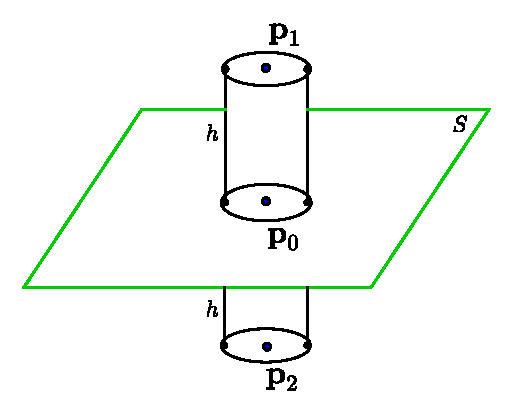
\includegraphics[scale=1]{interface_elastici}
\caption{\textit{Cilindro de dimens\~oes infinitesimais dividido pela interface separadora dos meios 1 e 2.}}
\label{fig.interface_elastici}
\end{figure}
Considerando ainda que cada um dos pontos $\mathbf{p}_1$ e $\mathbf{p}_2$ s\~ao os centros de cada uma das bases do cilindro, temos que os pontos $\mathbf{p}_0$, $\mathbf{p}_1$ e $\mathbf{p}_2$ est\~ao alinhados. Utilizando novamente a equa\c{c}\~ao \ref{eq.forca_total_3} e desprezando as for\c{c}as aplicadas na parede do cilindro (j\'a que vamos fazer $h\to 0$), temos que o equil\'ibrio de for\c{c}as aplicadas ao cilindro \'e dado por 
\begin{equation*}
\mathbf{F}=\mathbf{F}(\mathbf{p}_1)+\mathbf{F}(\mathbf{p}_2)+f
\end{equation*} 
onde $f$ \'e uma for\c{c}a de campo. Utilizando a segunda lei de Newton, utilizando a equa\c{c}\~ao \ref{eq.tensao_media} e desprezando as for\c{c}as de campo, temos
\begin{equation*}
\rho\,dh\,dA\frac{d\mathbf{v}}{dt}=\mathbf{T}(\mathbf{p}_1,\mathbf{n})dA+\mathbf{T}(\mathbf{p}_2,-\mathbf{n})dA.
\end{equation*} 
Fazendo o limite quando $h\to 0$ e mantendo constantes as \'areas das bases do cilindro, temos que os pontos $\mathbf{p}_i$ convergem para $\mathbf{p}_0$, e a equa\c{c}\~ao acima se torna
\begin{equation*}
\mathbf{T}(\mathbf{p}_0,\mathbf{n})-\mathbf{T}(\mathbf{p}_0,\mathbf{n})=\mathbf{0}.
\end{equation*}
Como o ponto $\mathbf{p}_0$ \'e tomado arbitrariamente, temos que o salto do tensor de tens\~oes ao longo da superf\'icie $S$ \'e nulo
\begin{equation*}
\left[\left[\mathbf{T}\right]\right]=\mathbf{0}.
\end{equation*}
Considerando um modelo onde uma camada n\~ao vai invadir a outra temos que a componente normal do vetor de deslocamento $\mathbf{u}\in S$ \'e nula. Da mesma forma, considerando que uma camada n\~ao desliza sobre a outra, temos que as componentes tangenciais de $\mathbf{u}$ tamb\'em s\~ao zero, e da\'i assumimos que o salto de $\mathbf{u}$ \'e nulo bem como sua velocidade,
\begin{equation*}
\left[\left[\mathbf{u}\right]\right]=\mathbf{0}\quad\text{e}\quad\left[\left[\frac{\partial}{\partial t}\mathbf{u}\right]\right]=\mathbf{0}.
\end{equation*}



\section{Generalizações da teoria}

\section{Conclusões}
%\chapter{Acoplamento Magneto-e\'alstico}

\section{Introdu\c{c}\~ao}

Como vimos na subse\c{c}\~ao \ref{sec.fund_eletr}, quando uma estrutura condutiva se movimenta num campo magn\'etico, uma corrente el\'etrica e um campo magn\'etico vari\'avel s\~ao gerados nessa estrutura. Segundo \cite{Mikhailenko_1997}, a passagem de uma onda s\'ismica pela subsuperf\'icie terrestre gera o movimento do material que comp\~oe essa subsuperf\'icie. Considerando que esse material \'e cont\'inuo e el\'astico, cont\'em uma certa distribui\c{c}\~ao de cargas el\'etricas e que o planeta Terra possui um campo geomagn\'etico natural, temos que o movimento relativo entre o material e o campo geomagn\'etico vai gerar varia\c{c}\~oes geomagn\'eticas locais associadas \`as ondas s\'ismicas que provocaram o movimento do material. Mais ainda, segundo \cite{Anisimov_1985} e \cite{Sadovsky_1980}, a onda eletromagn\'etica induzida \'e ''congelada`` \`a onda s\'ismica e se propaga n\~ao com a velocidade da luz, mas com a velocidade da onda $P$ ou da onda $S$, dependendo do tipo de onda s\'ismica, e podemos registrar e estudar essa varia\c{c}\~ao geomagn\'etica.
Um corpo nessas condi\c{c}\~oes \'e chamado de s\'olidos eletromagn\'etico-el\'asticos, essas varia\c{c}\~oes no campo geomagn\'etico s\~ao chamadas de \textit{ondas sismomagn\'eticas} e esse efeito recebeu o nome de \textit{efeito sismomagn\'etico} ou \textit{efeito magnetoel\'astico}.

Segundo \cite{erigen_1963}, \'e poss\'ivel investigar algumas intera\c{c}\~oes din\^amicas que podem ocorrer entre campos eletromagn\'eticos e campos el\'asticos em s\'olidos homog\^eneos e isotr\'opicos. Assim, esses autores desenvolveram um modelo matem\'atico de combina\c{c}\~ao entre a teoria de elasticidade infinitesimal e a teoria eletromagn\'etica linearizada, o qual ser\'a apresentado a seguir. A intera\c{c}\~ao se deve principalmente \`a for\c{c}a de corpo de Lorentz, \`a modifica\c{c}\~ao das equa\c{c}\~oes constitutivas e das condi\c{c}\~oes de contorno provocada pela velocidade do material, e \`as for\c{c}as superficiais introduzidas pelos campos.

\section{Equa\c{c}\~oes Constitutivas do Meio}
Seguindo a nota\c{c}\~ao apresentada em \cite{erigen_1963}, temos que os vetores eletromagn\'eticos que representam o meio de propaga\c{c}\~ao das ondas propriamnte dito s\~ao representados por $\mathbf{E}^0$, $\mathbf{D}^0$, $\mathbf{B}^0$, $\mathbf{H}^0$ e
$\mathbf{J}^0$. Essas mesmas quantidades, quando se referirem \`as medidas observadas em laborat\'orio s\~ao denotadas apenas retirando-se o sobre-escrito $0$. Transferindo essa nota\c{c}\~ao para as equa\c{c}\~oes \ref{eq.D_funcao_E} e \ref{eq.B_funcao_H} temos
\begin{equation}\label{eq.constitutivas_parciais}
\mathbf{D}^0=\epsilon\,\mathbf{E}^0\quad\text{e}\quad\mathbf{B}^0=\mu\,\mathbf{H}^0.
\end{equation}

Em muitos materiais, a densidade de corrente el\'etrica \'e linearmente dependente de um campo el\'etrico externo, e tal rela\c{c}\~ao, conhecida como a \textit{lei de Ohm}, pode ser escrita usando a nota\c{c}\~ao apresentada acima como
\begin{equation}\label{eq.lei_ohm}
\mathbf{J}^0=\sigma\,\mathbf{E}^0,
\end{equation}
onde $\sigma$ \'e a \textit{condutividade} do meio. As equa\c{c}\~oes \ref{eq.constitutivas_parciais} juntamente com a equa\c{c}\~ao \ref{eq.lei_ohm} s\~ao denominadas \textit{equa\c{c}\~oes eletromagn\'eticas contitutivas do meio}, quando o mesmo \'e isotr\'opico, homog\^eneo e se encontra em repouso. As mesmas equa\c{c}\~oes se mant\^em quando o meio se move por ocasi\~ao da passagem de uma onda s\'ismica. 


\section{Modelo de Dunkin e Erigen}






\section{Conclusões}
%\chapter{Recondicionamento do Modelo de Dunkin e Erigen}
Uma das contribui\c{c}\~oes dessa monografia \'e a utiliza\c{c}\~ao de hip\'oteses simplificadoras de ordem f\'isica e experimental, dispon\'iveis na literatura, para reeescrever o modelo do acoplamento magneto-el\'astico de forma que o mesmo possa receber um tratamento matem\'atico e computacional, no sentido de solucionar um problema direto.

Como vimos na subse\c{c}\~ao \ref{sec.magnetizacao_polarizacao}, a polariza\c{c}\~ao e magnetiza\c{c}\~ao de um determinado material depende das caracter\'isticas de cada material. De acordo com \cite{jackson_classical_1999} e \cite{griffiths}, as equa\c{c}\~oes constitutivas apresentadas na subse\c{c}\~ao \ref{sec.constitutivas_dunkin} podem n\~ao ser simples pois existe uma diversidade enorme de propriedades el\'etricas e magn\'eticas dos materias, especialmente em s\'olidos cristal\'inicos  e materias ferroel\'etricos e ferromagn\'eticos que t\^em polariza\c{c}\~ao e magnetiza\c{c}\~ao n\~ao nulos mesmo na absten\c{c}\~ao de aplica\c{c}\~ao de campos eletromagn\'eticos. Com excess\~ao desses tipos de materias, a aplica\c{c}\~ao de campos eletromagn\'eticos produzem polariza\c{c}\~ao e magnatiza\c{c}\~ao proporcional aos campos aplicados, e a rela\c{c}\~ao do campo de densidade de fluxo el\'etrico com o campo el\'etrico bem como a rela\c{c}\~ao do campo magn\'etico auxiliar com o campo magn\'etico s\~ao consideradas lineares, pois a contribui\c{c}\~ao das parcelas n\~ao-lineares tornam-se desprez\'iveis. Podemos ainda considerar a permeabilidade magn\'etica de muitos materiais tendo valor muito pr\'oximo da permeabilidade magn\'etica no v\'acuo, assim $\mu=\mu_0$. Com isso, temos que o escalar $\alpha$ definido em \ref{eq.constitutiva_1} tem seu valor considerado nulo, e as express\~oes para o campo de densidade de fluxo el\'etrico e o campo magn\'etico da subse\c{c}\~ao \ref{sec.constitutivas_dunkin} se tornam
\begin{align}\label{eq.constitutiva_alpha_1}
\mathbf{D}&=\epsilon\,\mathbf{E}\\\nonumber\\\label{eq.constitutiva_alpha_2}
\mathbf{B}&=\mu\,\mathbf{H}.
\end{align}
Substituindo a equa\c{c}\~ao \ref{eq.constitutiva_alpha_1} na equa\c{c}\~ao \ref{eq.campo_dunkin_1} e aplicando a transformada de Fourier, temos a rela\c{c}\~ao entre o campo el\'etrico e o campo magn\'etico auxiliar dada por
\begin{equation}
\nabla\times\mathbf{\widehat{E}}=i\,\omega\,\mu_0\mathbf{\widehat{H}},
\end{equation}
onde $i$ \'e um n\'umero complexo, $\omega$ \'e a frequ\^encia temporal e a nota\c{c}\~ao $\widehat{\,\,}$ significa que a fun\c{c}\~ao vetorial est\'a no dom\'inio da frequ\^encia temporal.

Ondas eletromagn\'eticas se propagam com velocidade da luz que \'e limitada. Segundo \cite{jackson_classical_1999}, num sistema onde as dimens\~oes s\~ao pequenas comparadas ao comprimento de onda eletromagn\'etica e comparadas \`a escala de tempo dominante, podemos tratar a velocidade da luz como instant\^anea num regime denominado \textit{quasi-estacion\'ario}. Como consequ\^encia dessa premissa, em meios condutivos a contribui\c{c}\~ao do campo de densidade de fluxo el\'etrico \'e muito pequena quando comparada \`a contribui\c{c}\~ao da densidade de corrente el\'etrica na produ\c{c}\~ao de campos magn\'eticos. Assim, podemos desprezar a parcela referente \`a corrente deslocada introduzida por Maxwell na lei de Amper\`e, o que implica (pela equa\c{c}\~ao \ref{eq.campo_dunkin_3}) em $\rho_e=0$. 
Vamos supor ainda que o campo magn\'etico auxiliar medido durante o efeito magneto-el\'astico seja uma combina\c{c}\~ao do campo magn\'etico gerado $\mathbf{H}$ mais o campo magn\'etico natural da Terra $\mathbf{H}^0$, e para manter a nota\c{c}\~ao vamos usar a substitui\c{c}\~ao 
\begin{equation}
\mathbf{H}\longrightarrow\mathbf{H}+\mathbf{H}^0.
\end{equation}
Utilizando a equa\c{c}\~ao \ref{eq.constitutiva_alpha_2}, o campo de densidade de corrente el\'etrica dado pela subse\c{c}\~ao \ref{sec.constitutivas_dunkin} poder ser reescrito como
\begin{equation}
\mathbf{J}=\sigma\,\mathbf{E}+\mathbf{v}\times\sigma\,\mu_0\mathbf{H}.
\end{equation}
Substituindo esta \'ultima rela\c{c}\~ao juntamente com a equa\c{c}\~ao \ref{eq.constitutiva_alpha_1} na equa\c{c}\~ao \ref{eq.campo_dunkin_2}, e aplicando a transformada de Fourier, temos
\begin{equation}
\nabla\times\mathbf{\widehat{H}}=(\sigma-i\,\epsilon\,\omega)\,\mathbf{\widehat{E}}+\mathbf{\widehat{v}}\times\sigma\mu_0\mathbf{H}^0,
\end{equation}
onde $\mathbf{\widehat{v}}=-i\,\omega\mathbf{\widehat{u}}$ \'e a velocidade de deslocamento do meio. Na dedu\c{c}\~ao da equa\c{c}\~ao acima, estamos considerando que a contribui\c{c}\~ao da parcela $\mathbf{\widehat{v}}\times\sigma\mu_0\mathbf{\widehat{H}}$ \'e desprez\'ivel se comparada \`a contribui\c{c}\~ao do campo geomagn\'etico, ainda como uma consequ\^encia do regime quasi-estacion\'ario.

De acordo com \cite{Knopoff_1955}, a altera\c{c}\~ao que o campos eletromagn\'eticos aplicam em ondas el\'asticas \'e desprez\'ivel, e assim podemos excluir a for\c{c}a de Lorentz e reescrever a equa\c{c}\~ao \ref{eq.campo_dunkin_5} no dom\'inio da frequ\^encia na forma matricial como 
\begin{equation}
-i\,\omega\rho\,\mathbf{\widehat{v}}=\nabla\cdot\widehat{\tau} + \mathbf{\widehat{F}}.
\end{equation}
A lei de Hooke dada na subse\c{c}\~ao \ref{sec.constitutivas_dunkin} pode ser reescrita no dom\'inio da frequ\^encia e em sua forma matricial como
\begin{equation}
\widehat{\tau}=\lambda\,\nabla\cdot\mathbf{\widehat{u}}\cdot\,I + \mu\,(\nabla\,\mathbf{\widehat{u}}+\nabla\mathbf{\widehat{u}}^\top),
\end{equation}
onde $I$ \'e a matriz identidade e $\nabla\mathbf{\widehat{u}}=(\nabla u_1,\nabla u_2,\nabla u_3)$ \'e o gradiente do campo vetorial que d\'a o deslocamento do meio de propaga\c{c}\~ao das ondas.

Substituindo a equa\c{c}\~ao \ref{eq.constitutiva_alpha_2} na equa\c{c}\~ao \ref{eq.campo_dunkin_4} e aplicando a transformada de Fourier, temos
\begin{equation}
\nabla\cdot\mathbf{\widehat{H}}=0.
\end{equation}

Assumindo as hip\'oteses simplificadoras acima, com a depend\^encia do tempo dada por $e^{(-i\,\omega\,t)}$, as equa\c{c}\~oes diferenciais parciais linearizadas de magneto-elasticidade s\~ao
\begin{align*}
\nabla\times\mathbf{\widehat{E}}&=i\,\omega\,\mu_0\mathbf{\widehat{H}}\\\\
\nabla\times\mathbf{\widehat{H}}&=(\sigma-i\,\epsilon\,\omega)\,\mathbf{\widehat{E}}+\mathbf{\widehat{v}}\times\sigma\mu_0\mathbf{H}^0\\\\
-i\,\omega\rho\,\mathbf{\widehat{v}}&=\nabla\cdot\widehat{\tau} + \mathbf{\widehat{F}}\\\\
\widehat{\tau}&=\lambda\,\nabla\cdot\mathbf{\widehat{u}}\cdot\,I + \mu\,(\nabla\,\mathbf{\widehat{u}}+\nabla\mathbf{\widehat{u}}^\top)\\\\
\nabla\cdot\mathbf{\widehat{H}}&=0
\end{align*}

Vamos definir $\sigma^*=(\sigma-i\,\epsilon\,\omega)$. No subsolo, por conta do regime quasi-estacion\'ario, $(\sigma>>\epsilon\,\omega)$  e  temos $\sigma^*=\sigma$. No ar, a condutividade \'e zero e a permeabilidade el\'etrica \'e pr\'oxima a do v\'acuo, assim temos $\sigma^*=-i\,\epsilon_0\omega$.
%\chapter{M\'etodo Matricial para Solu\c{c}\~ao de EDO's}

Este cap\'itulo trata do estudo do m\'etodo matricial para analisar a propaga\c{c}\~ao de ondas em subsuperf\'icie terrestre, conforme estruturado em \cite{Ursin-1983}. Gra\c{c}as a similaridade matem\'atica entre sistemas de EDP's eletromagn\'eticas (Maxwell) e sistemas de EDP's el\'asticas (Lamè), podemos dar um desenvolvimento unificado para esses sistemas. Utilizamos um conjunto de transformadas e mudan\c{c}a de eixos coordenados para dividir esses dois sistemas de EDP's em quatro sistemas de EDO's escritos em forma matricial, onde as vari\'aveis dependentes estejam em fun\c{c}\~ao apenas da profundidade e da frequ\^encia temporal. Os coeficientes desses sistemas de EDO's podem ser reunidos numa matriz $M$ de dimens\~ao $2n\times 2n$, a qual pode ser particionada em quatro submatrizes de dimens\~ao $n\times n$, e \'e usada como o ponto de partida para o estudo da propaga\c{c}\~ao de ondas em subsuperf\'icie.  

As propriedades de simetria da matriz $M$ nos permitem separar o campo de ondas em ascendentes e descendentes atrav\'es de uma decomposi\c{c}\~ao em autovetores. Essas propriedades nos permitem tamb\'em deduzir caracter\'isticas invariantes da propaga\c{c}\~ao, onde uma dessas caracter\'isticas \'e v\'alida apenas para meios de baixa dissipa\c{c}\~ao de ondas e correspondem \`a conserva\c{c}\~ao de energia. A matriz de propaga\c{c}\~ao de ondas pode ser computada para camadas homog\^eneas ou n\~ao, atrav\'es de um m\'etodo relativamente simples. Dado o vetor de ondas na camada superficial, podemos calcular seu valor para qualquer camada usando a matriz de propaga\c{c}\~ao.

A propaga\c{c}\~ao de ondas em meios estratificados produz fen\^omenos de transmiss\~ao e reflex\~ao de ondas. Dadas as dedu\c{c}\~oes das matrizes de transmiss\~ao e reflex\~ao, podemos relacion\'a-las com a matriz de propaga\c{c}\~ao, bem como deduzir propriedades de simetrias para essas matrizes atrav\'es das caracter\'isticas invariantes da propaga\c{c}\~ao. Podemos ainda deduzir as matrizes de transmiss\~ao e reflex\~ao modificadas para pilha de camadas limitadas superiormente por uma superf\'icie livre.

\section{Caracter\'isticas das Equa\c{c}\~oes na Forma Matricial de Ursin}

%Sendo $\mathbf{x}=(x,y,z)^{\top}$ o espa\c{c}o $\mathbb{R}^3$ e aplicando as tranformadas de Fourier direta e inversa na forma
%\begin{align*}
%F(\omega,k_1,k_2,z) &= \iiint_{-\infty}^{\infty}f(t,x,y,z)\,e^{i\omega t-ik_1x-ik_2y}dt\,dxdy\\\\
%f(t,x,y,z) &= \left(\frac{1}{2\,\pi}\right)^3\,\iiint_{-\infty}^{\infty}F(\omega,k_1,k_2,z)\,e^{-i\omega t+ik_1x+ik_2y}d\omega\,dk_1dk_2\,,
%\end{align*}
%podemos escrever um conjunto de EDP's que descevem a propaga\c{c}\~ao de ondas sismomagn\'eticas em camadas horizontais da subsuperf\'icie terrestre somente em fun\c{c}\~ao da profundidade $z$. 
%
%A t\'itulo de exemplo, tanto as EDP's de Maxwell para o eletromagnetismo
%\begin{align}\label{eq.faraday_ampere}\nonumber
%\nabla\times\mathbf{E}&=-\frac{\partial}{\partial t}\mathbf{B}\\\\\nonumber
%\nabla\times\mathbf{H}&=\sigma\mathbf{E}+\frac{\partial}{\partial t}\mathbf{D}+\mathbf{G}\,,
%\end{align}
%como as EDP's el\'asticas
%\begin{align}\label{eq.cauchy_hooke}\nonumber
%\rho\frac{\partial^2 \mathbf{U}}{\partial t^2}&=\nabla\cdot\tau+\mathbf{F}\\\\\nonumber
%\tau&=\lambda\nabla\cdot \mathbf{U}\cdot I + \mu(\nabla \mathbf{U}+\nabla \mathbf{U}^*)\,,
%\end{align}
%podem ser escritas no formato matricial apresentado por Ursin, ou seja, 
\'E poss\'ivel utilizar o m\'etodo matricial no formato preconizado por \cite{Ursin-1983} para resolver sistemas de EDO's desde que se possa escrever tal sistema como
\begin{align}\label{eq.matricial}
\frac{\partial\,\mathbf{\Phi}^{(m)}}{\partial\,z} &= -\,i\,\omega\,M^{(m)}\,\mathbf{\Phi}^{(m)}+\mathbf{S}^{(m)},\quad\text{com}\quad m\,\in\mathbb{N},
\end{align}
%\begin{bmatrix}
%\mathbf{\Phi_1}\\
%\mathbf{\Phi_2}	
%\end{bmatrix}\,,
onde $\mathbf{S}^{(m)}$ \'e um vetor de fonte de onda s\'ismica de dimens\~ao $2\,n_m$ e as matrizes $M^{(m)}_{2\,n_m\times2\,n_m}$ t\^em o formato
\begin{equation}\label{eq.matriz_M}
M^{(m)}
=
\begin{pmatrix}
\mathbf{0}&M_1^{(m)}\\
M_2^{(m)}&\mathbf{0}
\end{pmatrix},
\end{equation}
onde $M_1^{(m)}$ e $M_2^{(m)}$ s\~ao submatrizes sim\'etricas de dimens\~ao $n_m\times n_m$.

A equa\c{c}\~ao \ref{eq.matricial} tem as seguintes caracter\'isticas:
\begin{itemize}
\item $M^{(m)}_{2\,n\times2\,n}$ \'e uma matriz que pode ser particionada em quatro submatrizes $n\times n$, com submatrizes de zeros na diagonal principal e submatrizes sim\'etricas $M_1^{(m)}$ e $M_2^{(m)}$ na diagonal secund\'aria. As componentes de $M_1^{(m)}$ e $M_2^{(m)}$ s\~ao fun\c{c}\~oes dos par\^ametros das EDP's que est\~ao sendo trabalhadas, s\~ao fun\c{c}\~oes tamb\'em de $z$ e do vetor real de vagarosidade $\pmb{\gamma}=\frac{\mathbf{k}}{\omega}$. Para meios de baixa dissipa\c{c}\~ao das ondas, as matrizes $M_1^{(m)}$ e $M_2^{(m)}$ s\~ao reais; 
\item O vetor de onda $\mathbf{\Phi}^{(m)}$ tem dimens\~ao $2n\times1$ e \'e particionado em dois vetores $\mathbf{\Phi}^{(m)}_1$ e $\mathbf{\Phi}^{(m)}_2$ com dimens\~ao $n\times1$ . As componentes do vetor de onda s\~ao escolhidas de forma que $\mathbf{\Phi}^{(m)}$ seja cont\'inuo atrav\'es das fronteiras entre duas camadas;
\item  Para ondas el\'asticas, metade das componentes de $\mathbf{\Phi}^{(m)}$ s\~ao zeros na superf\'icie livre, ou seja, existe uma matriz de permuta\c{c}\~ao $T_{2n\times2n}$ onde $T^{-1}=T^\top$ e tal que
\begin{equation*}
\begin{bmatrix}
\mathbf{V}_1(\mathbf{0})\\
\mathbf{0}
\end{bmatrix}
=T\,\mathbf{\Phi}^{(m)}\quad\text{quando}\quad z = 0\,;
\end{equation*}
\item As componentes do vetor de onda $\mathbf{\Phi}^{(m)}$ s\~ao escolhidas de forma que o fluxo de energia na dire\c{c}\~ao $z$ seja dado por
\begin{equation*}
J=-\frac{1}{4}(\mathbf{\Phi}_1^{(m)\,H}\mathbf{\Phi}^{(m)}_2+\mathbf{\Phi}_2^{(m)\,H}\mathbf{\Phi}^{(m)}_1)=-\frac{1}{4}\mathbf{\Phi}^{(m)\,H}\,M_0\mathbf{\Phi}^{(m)}\,,
\end{equation*}
onde $H$ denota complexo conjugado transposto,
\begin{equation*}
M_0=
\begin{bmatrix}
0_{n\times n}&I\\
I&0_{n\times n}
\end{bmatrix}
\end{equation*}
e $I$ \'e uma matriz identidade $n\times n$.
\end{itemize}

O m\'etodo a seguir \'e aplicado em equa\c{c}\~oes escritas no formato matricial \ref{eq.matricial}, com ondas se propagando numa pilha de camadas homog\^eneas e assumimos que os par\^ametros das equa\c{c}\~oes s\~ao fun\c{c}\~oes cont\'inuas no interior de cada camada e que dependem apenas da profundidade $z$. O modelo inclui pilha de camadas homog\^eneas com par\^ametros constantes por camada e consideramos o eixo $z$ como sendo positivo no sentido descendente.

\section{Diagonaliza\c{c}\~ao}\label{sec.diagonalizacao}
Considere matrizes $M$ conforme a equa\c{c}\~ao \ref{eq.matriz_M}, onde por simplicidade de escrita n\~ao usaremos o sobrescrito $m$. Vamos aplicar nesta matriz um procedimento de diagonaliza\c{c}\~ao que pode ser encontrado em trabalhos como \cite{Ursin-1983}, \cite{White_Zhou_2006} e \cite{Azeredo_2013}.

Seja $(\mathbf{a}_m,\,\mathbf{b}_m)^\top$ seja um autovetor da matriz $M$ associado ao autovalor $q_m$, com $m=1,...,n$, assim
\begin{equation}
\begin{pmatrix}
0_{n\times n}&M_1\\
M_2&0_{n\times n}
\end{pmatrix}
\begin{pmatrix}
\mathbf{a}_m\\
\mathbf{b}_m
\end{pmatrix}
=
q_m\,
\begin{pmatrix}
\mathbf{a}_m\\
\mathbf{b}_m
\end{pmatrix}.
\end{equation}
Ou seja, 
\begin{equation}\label{eq.M1_b}
M_1\mathbf{b}_m=q_m\,\mathbf{a}_m 
\end{equation}
e
\begin{equation}\label{eq.M2_a}
M_2\mathbf{a}_m=q_m\,\mathbf{b}_m. 
\end{equation}
Multiplicando \ref{eq.M1_b} pela esquerda por $M_2$ e substituindo \ref{eq.M2_a}, temos
\begin{equation}\label{eq.m2m1bm}
M_2M_1\mathbf{b}_m=q_m^2\mathbf{b}_m.
\end{equation} 
Analogamente, multiplicando \ref{eq.M2_a} pela esquerda por $M_1$ substituindo \ref{eq.M1_b}, temos 
\begin{equation}\label{eq.m1m2am}
M_1M_2\mathbf{a}_m=q_m^2\mathbf{a}_m.
\end{equation}
Desta forma, $\mathbf{a}_m$ \'e um autovetor associado \`a matriz $M_1M_2$, e $\mathbf{b}_m$ \'e um autovetor associado \`a matriz $M_2M_1$. 

Como estamos assumindo que $M_1$ e $M_2$ s\~ao sim\'etricas, partindo da equa\c{c}\~ao \ref{eq.m2m1bm} e usando a equa\c{c}\~ao \ref{eq.m1m2am}, temos
\begin{align*}
q_m^2\mathbf{b}_m&=M_2M_1\mathbf{b}_m\\
q_m^2\mathbf{a}_j^\top\mathbf{b}_m&=\mathbf{a}_j^\top M_2M_1\mathbf{b}_m\\
&=\mathbf{b}_m^\top M_1M_2\mathbf{a}_j\\
&=q_j^2\mathbf{a}_j^\top\mathbf{b}_m.
\end{align*}
Isolando $\mathbf{a}_j^\top\mathbf{b}_m$ na \'ultima igualdade acima, temos que 
\begin{empheq}[left={\mathbf{a}_j^\top\mathbf{b}_m=\empheqlbrace}]{align}\label{eq.ajTbm}\nonumber
0\,,&\quad\text{se}\quad m\neq j\\\\\nonumber
\alpha_{j,m}\,,&\quad\text{se}\quad m=j,
\end{empheq}
onde $\alpha$ \'e um valor indeterminado.

Vamos definir a matriz $L_1$ de dimens\~ao $n\times n$ onde cuja $m$-\'esima coluna \'e dada por $\mathbf{a}_m$, e a matriz $L_2$ tamb\'em de dimens\~ao $n\times n$ cuja $m$-\'esima coluna \'e dada por $\mathbf{b}_m$. Assim, podemos reescrever as equa\c{c}\~oes \ref{eq.M1_b} e \ref{eq.M2_a}, respectivamente, como
\begin{align}\label{eq.m1l2}
M_1L_2&=L_1\Lambda\\\label{eq.m2l1}
M_2L_1&=L_2\Lambda,
\end{align}
onde a matriz $\Lambda_{n\times n}$ \'e a matriz diagonal dos autovalores. Observe que podemos trabalhar com as equa\c{c}\~oes normalizadas tomando $\alpha_{j,m}=1$ na equa\c{c}\~ao \ref{eq.ajTbm}, que passa a definir o s\'imbolo \textit{Delta de Kroneker}\footnote{Nos abstivemos de usar o caracter grego $\delta$ na equa\c{c}\~ao \ref{eq.ajTbm} por este j\'a definir a fun\c{c}\~ao Delta de Dirac em nosso escopo.}, conforme \cite{lebedev_2003}. Assim, escrevemos as componentes de $\Lambda$ como $\Lambda_{j,m}=q_j\mathbf{a}_j^\top\mathbf{b}_m$. Observe ainda que, deste modo, a equa\c{c}\~ao \ref{eq.ajTbm} define a matriz identidade $I_{n\times n}$, a qual podemos usar para mostrar que
\begin{align}\label{eq.l1l2}
L_1^{-1}&=L_2^\top\\\label{eq.l2l1}
L_2^{-1}&=L_1^\top.
\end{align}
Multiplicando pela direita as equa\c{c}\~oes \ref{eq.m1l2} e \ref{eq.m2l1} respectivamente por $L_2^{-1}$ e $L_1^{-1}$, e substituindo as equa\c{c}\~oes \ref{eq.l1l2} e \ref{eq.l2l1}, temos
\begin{align}
M_1&=L_1\Lambda L_1^\top\\
M_2&=L_2\Lambda L_2^\top.
\end{align}
Definindo a matriz $L_{2\,n\times 2\,n}$ como
\begin{equation}\label{eq.matriz_L}
L=\frac{1}{\sqrt{2}}
\begin{pmatrix}
L_1&L_1\\
L_2&-L_2
\end{pmatrix},
\end{equation}
e a matriz $\tilde{\Lambda}$ como
\begin{equation}\label{eq.tildeLambda}
\tilde{\Lambda}=
\begin{pmatrix}
\Lambda&0\\
0&-\Lambda
\end{pmatrix},
\end{equation}
podemos deduzir que
\begin{equation}\label{eq.L^-1}
L^{-1}=\frac{1}{\sqrt{2}}
\begin{pmatrix}
L_2^\top&L_1^\top\\
L_2^\top&-L_1^\top
\end{pmatrix}
\end{equation}
e
\begin{equation}\label{eq.m_semelhante_lambda}
M=L\,\tilde{\Lambda}\,L^{-1}.
\end{equation}

\section{Solu\c{c}\~ao de EDO's na Aus\^encia de Fonte}\label{sec.ausencia_fonte}

Vamos determinar inicialmente a solu\c{c}\~ao de EDO's  considerando o meio homog\^eneo e livre de fonte de onda s\'ismica. Ap\'os a diagonaliza\c{c}\~ao dessas equa\c{c}\~oes, podemos aplicar um m\'etodo utilizado por alguns autores como \cite{Ursin-1983}, \cite{Azeredo_2013}, \cite{White_Zhou_2006}, \cite{miranda_2016} entre outros, para determinar as solu\c{c}\~oes na aus\^encia de fonte. Esse mesmo m\'etodo pode ser utilizado para determinar as solu\c{c}\~oes na presen\c{c}a de fonte como veremos no cap\'itulo \ref{sec.presenca_fonte}. Aus\^encia de fonte significa que temos $\mathbf{S}^{(m)}=0$ na equa\c{c}\~ao \ref{eq.matricial}. A matriz ${M}^{(m)}$ possui entradas constantes por camada estratigr\'afica, as submatrizes na diagonal principal s\~ao nulas e as submatrizes na diagonal secund\'aria s\~ao sim\'etricas. 

\subsection{Ondas Ascendentes e Ondas Descendentes}

Vamos redefinir o vetor de ondas como
\begin{equation}\label{eq.Phi}
\mathbf{\Phi}=L\,\mathbf{\Psi}.
\end{equation}
Substituindo a equa\c{c}\~ao \ref{eq.Phi} na equa\c{c}\~ao \ref{eq.matricial}, temos
\begin{equation}\label{eq.matricial_sem_fonte}
\frac{\partial\,\mathbf{\Psi}}{\partial\,z} =-\,i\,\omega\,L^{-1}M\,L\,\mathbf{\Psi},
\end{equation}
onde o sobrescrito $m$ est\'a sendo omitido por quest\~ao de simplicidade.
De acordo com a equa\c{c}\~ao \ref{eq.m_semelhante_lambda}, temos que as matrizes $M$ e $\tilde{\Lambda}$ s\~ao semelhantes, assim
\begin{equation*}
\tilde{\Lambda}=L^{-1}M\,L.
\end{equation*}
Substituindo $\tilde{\Lambda}$ na equa\c{c}\~ao \ref{eq.matricial_sem_fonte}, temos
\begin{equation}\label{eq.matricial_sem_fonte_2}
\frac{\partial\,\mathbf{\Psi}}{\partial\,z} =-\,i\,\omega\,\tilde{\Lambda}\,\mathbf{\Psi}.
\end{equation}
De acordo com a equa\c{c}\~ao \ref{eq.tildeLambda}, $\tilde{\Lambda}$ \'e uma matriz cuja diagonal principal cont\'em a submatriz $\Lambda$, onde $\Lambda$ \'e uma matriz diagonal contendo os autovalores $q_i$.
Definindo
\begin{equation}\label{eq.definicao_psi}
\mathbf{\Psi}=
\begin{pmatrix}
\mathbf{U}\\
\mathbf{D}
\end{pmatrix}
\end{equation}
e usando o fato de que $\tilde{\Lambda}$ \'e uma matriz diagonal, podemos resolver a equa\c{c}\~ao diferencial \ref{eq.matricial_sem_fonte_2} e expressar a solu\c{c}\~ao na forma
\begin{align}\nonumber
\mathbf{\Psi}(z)&=e^{-i\,\omega\,\tilde{\Lambda}(z-z_0)}\mathbf{\Psi}(z_0)\\\label{eq.solucao_psi}
&=\begin{pmatrix}
e^{-i\,\omega\,\Lambda(z-z_0)}\,\mathbf{U}(z_0)\\
e^{i\,\omega\,\Lambda(z-z_0)}\,\,\,\mathbf{D}(z_0)
\end{pmatrix}.
\end{align}
Desta maneira, $\mathbf{U}$ representa ondas ascendentes e $\mathbf{D}$ representa ondas descendentes, $z_0$ \'e um ponto fixo na mesma regi\~ao livre de fonte de $z$ e $e^{\pm i\,\omega\,\Lambda(z-z_0)}$ \'e uma matriz diagonal onde o $j$-ésimo elemento da diagonal principal \'e dado por $e^{\pm i\,\omega\,q_j(z-z_0)}$. 

\subsection{Matriz de Salto para Camadas Estratificadas}

A profundidade onde encontra-se uma interface entre duas camadas estratificadas ser\'a denotada por $\overline{z}$, onde as quantidades avaliadas imediatamente abaixo da interface ser\'a denotada por $\overline{z}^+$ e as quantidades avaliadas imediatamente acima da interface ser\'a denotada por $\overline{z}^-$.
De acordo com \cite{White_Zhou_2006}, temos a continuidade de $\mathbf{\Phi}$ atrav\'es das fronteiras entre as camadas, assim \'e v\'alida a rela\c{c}\~ao $\mathbf{\Phi}^+=\mathbf{\Phi}^-$. Substituindo a equa\c{c}\~ao \ref{eq.Phi}, temos 
\begin{align}\nonumber
L^+\mathbf{\Psi}^+&=L^-\mathbf{\Psi}^-\\\nonumber
\mathbf{\Psi}^+&=(L^+)^{-1}L^-\mathbf{\Psi}^-\\\label{eq.psi_matriz_salto}
\mathbf{\Psi}^+&=J\,\mathbf{\Psi}^-,
\end{align}
onde $J=(L^+)^{-1}L^-$ \'e denominada \textit{matriz de salto}. Substituindo a equa\c{c}\~ao \ref{eq.matriz_L}, podemos expressar a matriz de salto como
\begin{equation}
J=
\begin{pmatrix}
J_A&J_B\\
J_B&J_A
\end{pmatrix},
\end{equation}
onde $J_A$ e $J_B$ s\~ao dadas por
\begin{align}\label{eq.j_a}
J_A&=\frac{1}{2}\left[(L_2^+)^\top L_1^-+(L_1^+)^\top L_2^-\right]\\\label{eq.j_b}
J_B&=\frac{1}{2}\left[(L_2^+)^\top L_1^--(L_1^+)^\top L_2^-\right].
\end{align}
Com outra simples multiplica\c{c}\~ao de matrizes temos que
\begin{align}\nonumber
J^{-1}&=(L^-)^{-1}L^+\\\label{eq.inversa_matriz_salto}
&=
\begin{pmatrix}
J_A^\top&-J_B^\top\\
-J_B^\top&J_A^\top
\end{pmatrix}.
\end{align}

\subsection{Matriz de Reflex\~ao e Matriz de Transmiss\~ao}

Considere um meio estratificado, homog\^eneo no interior de cada camada, com $N$ interfaces nas profundidades $0<z_1<z_2<...<z_N<\infty$ e sem exist\^encia de fonte nessas camadas. 

\subsubsection{Reflex\~ao e Transmiss\~ao na \'Ultima Interface}
Pela figura \ref{fig.ondas_em_zn}, considerando que n\~ao h\'a ondas ascendentes depois da \'ultima interface em $z=z_N$, podemos substituir a defini\c{c}\~ao \ref{eq.definicao_psi} na equa\c{c}\~ao \ref{eq.psi_matriz_salto} e obter
\begin{align*}
\mathbf{\Psi}_N^-&=J_N^{-1}\,\mathbf{\Psi}_N^+\\\\
\begin{pmatrix}
\mathbf{U}_N^-\\
\mathbf{D}_N^-
\end{pmatrix}
&=J_N^{-1}\,
\begin{pmatrix}
0\\
\mathbf{D}_N^+
\end{pmatrix}.
\end{align*}

\begin{figure}
\centering
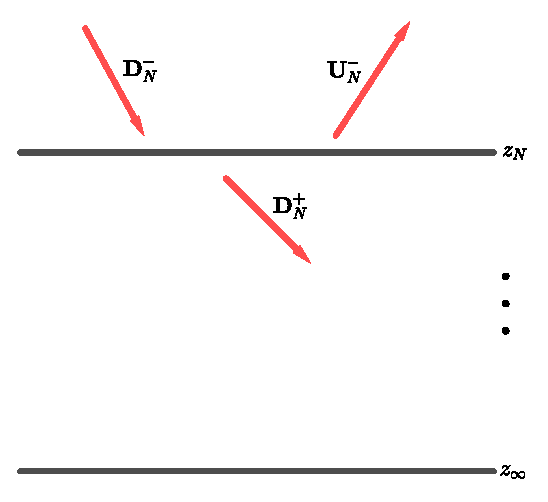
\includegraphics[scale=1]{ondas_em_zn}
\caption{\textit{Ondas ascendentes e descendentes na \'ultima interface. Observe que n\~ao h\'a ondas ascendentes depois da \'ultima camada}.}
\label{fig.ondas_em_zn}
\end{figure}

Substituindo a equa\c{c}\~ao \ref{eq.inversa_matriz_salto} na equa\c{c}\~ao anterior, temos
\begin{align*}
\begin{pmatrix}
\mathbf{U}_N^-\\
\mathbf{D}_N^-
\end{pmatrix}
&=
\begin{pmatrix}
J_{A,N}^\top&-J_{B,N}^\top\\
-J_{B,N}^\top&J_{A,N}^\top
\end{pmatrix}
\,
\begin{pmatrix}
0\\
\mathbf{D}_N^+
\end{pmatrix}\\\\
&=
\begin{pmatrix}
-J_{B,N}^\top \mathbf{D}_N^+\\
 J_{A,N}^\top \mathbf{D}_N^+
\end{pmatrix},
\end{align*}
ou seja,
\begin{align*}
\mathbf{U}_N^-&=-J_{B,N}^\top J_{A,N}^{-\top}\mathbf{D}_N^-\\
\mathbf{D}_N^+&=J_{A,N}^{-\top}\mathbf{D}_N^-.
\end{align*}
Assim, vemos que para computar uma onda refletida, ou seja, uma onda ascendente a partir de uma interface entre camadas, usamos uma \textit{matriz de reflex\~ao} que fica definida como
\begin{equation}\label{eq.reflexao_N}
\Gamma_N=-J_{B,N}^\top J_{A,N}^{-\top}.
\end{equation} 
Analogamente, vemos que para computar uma onda transmitida, ou seja, uma onda descendente a partir de uma interface entre camadas, usamos uma \textit{matriz de transmiss\~ao} que fica definida como
\begin{equation}\label{eq.transmissao_N}
T_N=J_{A,N}^{-\top}.
\end{equation} 

\subsubsection{Reflex\~ao e Transmiss\~ao numa Interface Qualquer}
Definimos a espessura de uma camada, a partir da interface superior, como
\begin{equation}
\Delta\,z_m=z_{m+1}-z_m,\qquad m=1,2,...,N-1,
\end{equation}
e temos que uma onda se propagando da interface na profundidade $z_m$ at\'e a interface em $z_{m+1}$ percorre uma profundidade total $\Delta\,z_m$. O valor dessa onda no fim da trajet\'oria, quando $z=z_{m+1}$, \'e aproximadamente igual a $\mathbf{\Psi}^-_{m+1}$, conforme a figura \ref{fig.N_interfaces}. Assim, usando a solu\c{c}\~ao \ref{eq.solucao_psi} podemos escrever
\begin{equation}\label{eq.solucao_delta_zm}
\mathbf{\Psi}^-_{m+1}=e^{-i\,\omega\tilde{\Lambda}_m\Delta\,z_m}\mathbf{\Psi}^+_m.
\end{equation}

\begin{figure}
\centering
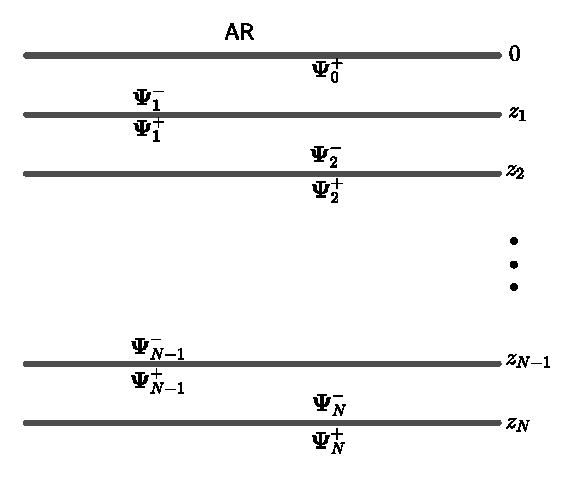
\includegraphics[scale=1]{n_interfaces}
\caption{\textit{Visualiza\c{c}\~ao de $N$ interfaces em subsuperf\'icie e a nota\c{c}\~ao das ondas nas proximadades de cada interface.}}
\label{fig.N_interfaces}
\end{figure}

Sabendo que essa onda se propagando na camada abaixo da interface em $z_m$ veio da camada anterior, podemos usar a matriz de salto na equa\c{c}\~ao \ref{eq.psi_matriz_salto} e escrever
\begin{align}\label{eq.salto_m}
\mathbf{\Psi}^+_{m}&=J_m\,\mathbf{\Psi}^-_m.
\end{align}
Substituindo a equa\c{c}\~ao \ref{eq.salto_m} na equa\c{c}\~ao \ref{eq.solucao_delta_zm}, temos
\begin{align}\label{eq.psi_m-}\nonumber
\mathbf{\Psi}^-_{m+1}&=e^{-i\,\omega\tilde{\Lambda}_m\Delta\,z_m}\mathbf{\Psi}^+_m\\\nonumber
\mathbf{\Psi}^-_{m+1}&=e^{-i\,\omega\tilde{\Lambda}_m\Delta\,z_m}J_m\,\mathbf{\Psi}^-_m\\
\mathbf{\Psi}^-_m&=J^{-1}_me^{i\,\omega\tilde{\Lambda}_m\Delta\,z_m}\mathbf{\Psi}^-_{m+1}
\end{align}
Substituindo a equa\c{c}\~ao \ref{eq.definicao_psi} e a equa\c{c}\~ao \ref{eq.inversa_matriz_salto} na equa\c{c}\~ao \ref{eq.psi_m-}, temos
\begin{align}\label{eq.refle_trans_1}
\mathbf{U}_m^-&=J^\top_{A,m}e^{i\,\omega\Lambda_m\Delta\,z_m}\mathbf{U}^-_{m+1}-J^\top_{B,m}e^{-i\,\omega\Lambda_m\Delta\,z_m}\mathbf{D}^-_{m+1}\\\nonumber\\\label{eq.refle_trans_2}
\mathbf{D}_m^-&=-J^\top_{B,m}e^{i\,\omega\Lambda_m\Delta\,z_m}\mathbf{U}^-_{m+1}+J^\top_{A,m}e^{-i\,\omega\Lambda_m\Delta\,z_m}\mathbf{D}^-_{m+1}.
\end{align}
Assim como definimos matriz de reflex\~ao para a \'ultima interface em $z_N$, podemos definir a matriz de reflex\~ao para uma interface qualquer, ou seja,
\begin{equation}\label{eq.reflexao_m+1}
\mathbf{U}^-_{m+1}=\Gamma_{m+1}\mathbf{D}^-_{m+1}.
\end{equation}
Substituindo a equa\c{c}\~ao \ref{eq.reflexao_m+1} na equa\c{c}\~ao \ref{eq.refle_trans_1} e na equa\c{c}\~ao \ref{eq.refle_trans_2}, temos
\begin{align}\label{eq.refle_trans_3}
\mathbf{U}_m^-&=(J^\top_{A,m}e^{i\,\omega\Lambda_m\Delta\,z_m}\Gamma_{m+1}-J^\top_{B,m}e^{-i\,\omega\Lambda_m\Delta\,z_m})\mathbf{D}^-_{m+1}\\\nonumber\\\label{eq.refle_trans_4}
\mathbf{D}_m^-&=(-J^\top_{B,m}e^{i\,\omega\Lambda_m\Delta\,z_m}\Gamma_{m+1}+J^\top_{A,m}e^{-i\,\omega\Lambda_m\Delta\,z_m})\mathbf{D}^-_{m+1}\,.
\end{align}
Substituindo a equa\c{c}\~ao \ref{eq.refle_trans_4} na equa\c{c}\~ao \ref{eq.refle_trans_3}, temos
\begin{align*}
\mathbf{U}_m^-&=(J^\top_{A,m}e^{i\,\omega\Lambda_m\Delta\,z_m}\Gamma_{m+1}-J^\top_{B,m}e^{-i\,\omega\Lambda_m\Delta\,z_m})\\
&\,\,\cdot\,\,(-J^\top_{B,m}e^{i\,\omega\Lambda_m\Delta\,z_m}\Gamma_{m+1}+J^\top_{A,m}e^{-i\,\omega\Lambda_m\Delta\,z_m})^{-1}\mathbf{D}_m^-\,,
\end{align*}
de onde podemos concluir que a matriz de reflex\~ao em uma interface em $z_m$ qualquer \'e dada por
\begin{align*}
\Gamma_{m}&=(J^\top_{A,m}e^{i\,\omega\Lambda_m\Delta\,z_m}\Gamma_{m+1}-J^\top_{B,m}e^{-i\,\omega\Lambda_m\Delta\,z_m})\\
&\,\,\cdot\,\,(-J^\top_{B,m}e^{i\,\omega\Lambda_m\Delta\,z_m}\Gamma_{m+1}+J^\top_{A,m}e^{-i\,\omega\Lambda_m\Delta\,z_m})^{-1},
\end{align*}
ou
\begin{align}\nonumber
\Gamma_{m}&=(J^\top_{A,m}e^{i\,\omega\Lambda_m\Delta\,z_m}\Gamma_{m+1}e^{i\,\omega\Lambda_m\Delta\,z_m}-J^\top_{B,m})\\\label{eq.matriz_reflexao_m}
&\,\,\cdot\,\,(-J^\top_{B,m}e^{i\,\omega\Lambda_m\Delta\,z_m}\Gamma_{m+1}e^{i\,\omega\Lambda_m\Delta\,z_m}+J^\top_{A,m})^{-1}.
\end{align}
Quando uma onda atinge uma interface, al\'em da possibilidade de reflex\~ao h\'a tamb\'em a possibilidade de trasmiss\~ao da onda para a camada inferior. De maneira an\'aloga ao desenvolvido para reflex\~ao de ondas, podemos deduzir a matriz para a transmiss\~ao de ondas em uma interface qualquer, que \'e dada por
\begin{equation}\label{eq.matriz_transmissao_m}
T_m=T_{m+1}e^{i\,\omega\,\Lambda\Delta\,z_m}(-J^\top_{B,m}e^{i\,\omega\Lambda_m\Delta\,z_m}\Gamma_{m+1}e^{i\,\omega\Lambda_m\Delta\,z_m}+J^\top_{A,m})^{-1}.
\end{equation}
A validade das equa\c{c}\~oes \ref{eq.matriz_reflexao_m} e \ref{eq.matriz_transmissao_m} para qualquer interface pode ser demonstrada por indu\c{c}\~ao sobre $m$, e todas as matrizes de reflex\~ao e transmiss\~ao podem ser computadas por recurss\~ao partindo das equa\c{c}\~oes \ref{eq.reflexao_N} e \ref{eq.transmissao_N}.

\section{Solu\c{c}\~ao na Presen\c{c}a de Fonte}\label{sec.presenca_fonte}
Em prospec\c{c}\~ao de petr\'oleo s\~ao utilizadas alguns tipos de fontes de ondas, atrav\'es das quais se faz um mapeamento das caracter\'isticas das camadas de subsuperf\'icie. Segundo \cite{dobrin_88}, esses tipos de fontes podem ser uma queda de peso, um caminh\~ao \textit{vibroseis}, explosivos e canh\~ao de ar, esta \'ultima fonte utilizada em prospec\c{c}\~ao mar\'itima. Sendo assim, vamos desenvolver uma solu\c{c}\~ao para o nosso problema considerando agora a presen\c{c}a de uma fonte.

Considere ainda a equa\c{c}\~ao \ref{eq.matricial} com o sobrescrito $m$ omitido. Uma fonte $\mathbf{S}$ localizada numa profundidade $z_s$ pode ser representada na forma
\begin{equation}\label{eq.fonte_geral}
\mathbf{S}=\mathbf{S}_0\delta(z-z_s)+\mathbf{S}_1\delta^\prime(z-z_s),
\end{equation}
onde $\mathbf{S}_0$ e $\mathbf{S}_1$ n\~ao dependem da profundidade e $\delta$ \'e a fun\c{c}ao \textit{Delta de Dirac} conforme a subse\c{c}\~ao \ref{sec.dirac}. Fontes que s\~ao distribu\'idas ao longo da profundidade podem, geralmente, ser sintetizadas por superposi\c{c}\~ao de fontes do tipo $\mathbf{S}_0$ e $\mathbf{S}_1$. 

Uma solu\c{c}\~ao por ser escrita como a combina\c{c}\~ao de uma solu\c{c}\~ao inicial sofrendo a a\c{c}\~ao de alguma fonte, ou seja,
\begin{equation}\label{eq.solucao_inicial_fonte}
\mathbf{\Phi}=\mathbf{\Phi}_0+\mathbf{S}_1\delta(z-z_s).
\end{equation} 
Substituindo a equa\c{c}\~ao \ref{eq.solucao_inicial_fonte} e a equa\c{c}\~ao \ref{eq.fonte_geral} na equa\c{c}\~ao \ref{eq.matricial}, temos
\begin{equation}\label{eq.matricial_fonte}
\frac{d\,\mathbf{\Phi}_0}{d\,z}=-i\,\omega\,M\,\mathbf{\Phi}_0+\left[\mathbf{S}_0-i\,\omega\,M\,\mathbf{S}_1\right]\,\delta(z-z_s),
\end{equation}
e por simplicidade, vamos escrever
\begin{equation}\label{eq.fonte_simplificada}
i\,\omega\,M\,\mathbf{S}_1-\mathbf{S}_0=
\begin{pmatrix}
\mathbf{S}_A\\
\mathbf{S}_B
\end{pmatrix}.
\end{equation}
Considerando a exist\^encia de uma interface imagin\'aria na profundidade $z_s$ da fonte, podemos determinar as condi\c{c}\~oes de salto no local da fonte da mesma forma que estudamos as condi\c{c}\~oes de salto nas interfaces que separam as camadas. Assim, integrando a equa\c{c}\~ao \ref{eq.matricial_fonte} no intervalo que come\c{c}a imediatamente acima da interface imagin\'aria da fonte $z_s^-$, e termina imediatamente abaixo da interface imagin\'aria da fonte em $z_s^+$, e substituindo a equa\c{c}\~ao \ref{eq.fonte_simplificada}, temos como solu\c{c}\~ao
\begin{equation*}
\mathbf{\Phi}_0(z_s^-)=\mathbf{\Phi}_0(z_s^+)+
\begin{pmatrix}
\mathbf{S}_A\\
\mathbf{S}_B
\end{pmatrix}.
\end{equation*}
Substituindo a equa\c{c}\~ao \ref{eq.solucao_inicial_fonte} e considerando as caracter\'isticas da fun\c{c}\~ao Delta de Dirac, temos a seguinte condi\c{c}\~ao de salto na profundidade da fonte
\begin{equation}\label{eq.salto_zs}
\mathbf{\Phi}(z_s^-)=\mathbf{\Phi}(z_s^+)+
\begin{pmatrix}
\mathbf{S}_A\\
\mathbf{S}_B
\end{pmatrix}.
\end{equation}

Vamos agora inserir uma interface imagin\'aria imediatamente abaixo da fonte, em $z=z_s^+$ e utilizar os m\'etodos do cap\'itulo \ref{sec.ausencia_fonte} para computar a matriz de reflex\~ao $\Gamma_s\equiv\Gamma(z_s^+)$ a partir do topo desta camada. J\'a que a interface em $z_s^+$ \'e fict\'icia, as propriedades do meio s\~ao iguais acima e abaixo dessa interface, assim temos que $L_2^+=L_2^-$ e $L_1^+=L_1^-$. Substituindo essas identidades nas equa\c{c}\~oes \ref{eq.j_a} e \ref{eq.j_b}, temos
\begin{align}\label{eq.j_a_ficticia}
J_A&=\frac{1}{2}\left[(L_2)^\top L_1+(L_1)^\top L_2\right]\\\label{eq.j_b_ficticia}
J_B&=\frac{1}{2}\left[(L_2)^\top L_1-(L_1)^\top L_2\right].
\end{align}
Substituindo as equa\c{c}\~oes \ref{eq.l1l2} e \ref{eq.l2l1} nas equa\c{c}\~oes \ref{eq.j_a_ficticia} e \ref{eq.j_b_ficticia}, obtemos que
\begin{align*}
J_A&=I\\
J_B&=0.
\end{align*}
Desta forma, a onda ascendente $\mathbf{U}(z_s^+)$ e a onda descendente $\mathbf{D}(z_s^+)$ a partir da interface em $z_s^+$ podem ser introduzidas na equa\c{c}\~ao \ref{eq.definicao_psi} para obtermos
\begin{equation*}
\mathbf{\Psi}(z_s^+)=
\begin{pmatrix}
\mathbf{U}(z_s^+)\\
\mathbf{D}(z_s^+)
\end{pmatrix}.
\end{equation*}
Substituindo a equa\c{c}\~ao \ref{eq.reflexao_m+1} na equa\c{c}\~ao acima, temos
\begin{equation}\label{eq.Psi_descendente}
\mathbf{\Psi}(z_s^+)=
\begin{pmatrix}
\Gamma_s\mathbf{D}(z_s^+)\\
\mathbf{D}(z_s^+)
\end{pmatrix},
\end{equation}
pois as ondas est\~ao numa mesma camada e da\'i usamos que
\begin{align*}
\mathbf{U}^-(z_s^+)&=\mathbf{U}(z_s^+)\\
\mathbf{D}^-(z_s^+)&=\mathbf{D}(z_s^+).
\end{align*}
Multiplicando a equa\c{c}\~ao \ref{eq.salto_zs} por $L^{-1}$ e substituindo a equa\c{c}\~ao \ref{eq.Phi}, obtemos
\begin{equation}\label{eq.Psi_salto_zs}
\mathbf{\Psi}(z_s^-)=\mathbf{\Psi}(z_s^+)+L^{-1}
\begin{pmatrix}
\mathbf{S}_A\\
\mathbf{S}_B
\end{pmatrix}.
\end{equation}
Substituindo a express\~ao para $L^{-1}$ dada pela equacao \ref{eq.L^-1}, juntamente com a equa\c{c}\~ao \ref{eq.Psi_descendente} na equa\c{c}\~ao \ref{eq.Psi_salto_zs}, temos
\begin{equation}\label{eq.solucao_phi_zs-}
\mathbf{\Psi}(z_s^-)=
\begin{pmatrix}
\Gamma_s\mathbf{D}(z_s^+)\\
\mathbf{D}(z_s^+)
\end{pmatrix}
+
\frac{1}{\sqrt{2}}\,
\begin{pmatrix}
L_2^\top\mathbf{S}_A+L_1^\top\mathbf{S}_B\\
L_2^\top\mathbf{S}_A-L_1^\top\mathbf{S}_B
\end{pmatrix}.
\end{equation}
Admitindo que a fonte esteja no interior da primeira camada, ou seja, $0<z_s<z_1$, a solu\c{c}\~ao dada pela equa\c{c}\~ao \ref{eq.solucao_phi_zs-} \'e propagada para cima a partir de $z_s^-$ usando a equa\c{c}\~ao \ref{eq.solucao_psi}, e o salto atrav\'es das interfaces entre camadas \'e dado pela equa\c{c}\~ao \ref{eq.psi_matriz_salto} at\'e que a onda atinja a interface terra/ar em $z=0^+$. Assim,
\begin{equation*}
\mathbf{\Psi}(0^+)=e^{-i\,\omega\,\tilde{\mathbf{\Lambda}}\,(0^+-z_s^-)}\,\mathbf{\Psi}(z_s^-),
\end{equation*}
e podemos usar as $n$ condi\c{c}\~oes de fronteira em $z=0$ para determinarmos as $n$ inc\'ognitas de $\mathbf{D}_s$. Os demais termos da solu\c{c}\~ao s\~ao conhecidos. A diferen\c{c}a $z_s^--0^+$ corresponde \`a profundidade da fonte, assim a solu\c{c}\~ao anterior pode ser reescrita como
\begin{align*}
\mathbf{\Psi}(0^+)&=e^{-i\,\omega\,\tilde{\mathbf{\Lambda}}\,(-z_s)}\,\mathbf{\Psi}(z_s^-)\\\\
\mathbf{\Psi}(0^+)&=
\begin{pmatrix}
e^{i\,\omega\,\mathbf{\Lambda}\,z_s}&\mathbf{0}\\
\mathbf{0}&e^{-i\,\omega\,\mathbf{\Lambda}\,z_s}
\end{pmatrix}
\mathbf{\Psi}(z_s^-).
\end{align*}
Substituindo a equa\c{c}\~ao \ref{eq.solucao_phi_zs-} na equa\c{c}\~ao acima, temos
\begin{equation}\label{eq.Psi_zero+}
\mathbf{\Psi}(0^+)=
\begin{pmatrix}
e^{i\,\omega\,\mathbf{\Lambda}\,z_s}\,\Gamma_s\mathbf{D}(z_s^+)\\
e^{-i\,\omega\,\mathbf{\Lambda}\,z_s}\,\mathbf{D}(z_s^+)
\end{pmatrix}
+
\frac{1}{\sqrt{2}}\,
\begin{pmatrix}
e^{i\,\omega\,\mathbf{\Lambda}\,z_s}\,(L_2^\top\mathbf{S}_A+L_1^\top\mathbf{S}_B)\\
e^{-i\,\omega\,\mathbf{\Lambda}\,z_s}\,(L_2^\top\mathbf{S}_A-L_1^\top\mathbf{S}_B)
\end{pmatrix},
\end{equation}
e teremos os valores de cada campo quando as ondas retornarem \`a superf\'icie.



%%\chapter{Solu\c{c}\~ao das Equa\c{c}\~oes \ref{eq.matricial_1}-\ref{eq.matricial_4} na Aus\^encia de Fonte}\label{sec.ausencia_fonte}

Vamos determinar inicialmente a solu\c{c}\~ao das equa\c{c}\~oes \ref{eq.matricial_1}-\ref{eq.matricial_4} considerando o meio homog\^eneo e livre de fonte de onda sismica. Apos a diagonalizacao dessas equacoes, podemos aplicar um m\'etodo utilizado por alguns autores como \cite{Ursin-1983}, \cite{Azeredo_2013}, \cite{White_Zhou_2006}, \cite{miranda_2016} entre outros, para determinar as solu\c{c}\~oes na aus\^encia de fonte. Esse mesmo metodo pode ser utilizado para determinar as solucoes na presenca de fonte como veremos no capitulo \ref{sec.presenca_fonte}. Aus\^encia de fonte significa que temos $\mathbf{S}^{(m)}=0$ para $m=1,2,3,4\,$ na equa\c{c}\~ao \ref{eq.matricial}. A matriz $\mathbf{M}^{(m)}$ \'e constante onde as submatrizes na diagonal principal s\~ao nulas e as submatrizes na diagonal secund\'aria s\~ao sim\'etricas. 



\section{Ondas Ascendentes e Ondas Descendentes}

Vamos redefinir o vetor de ondas como
\begin{equation}\label{eq.Phi}
\mathbf{\Phi}=L\,\mathbf{\Psi}.
\end{equation}
Substituindo a equa\c{c}\~ao \ref{eq.Phi} na equa\c{c}\~ao \ref{eq.matricial}, temos
\begin{equation}\label{eq.matricial_sem_fonte}
\frac{\partial\,\mathbf{\Psi}}{\partial\,z} =-\,i\,\omega\,L^{-1}M\,L\,\mathbf{\Psi},
\end{equation}
onde o sobrescrito $m$ est\'a sendo omitido por quest\~ao de simplicidade.
De acordo com a subse\c{c}\~ao \ref{sec.diagonalizacao_ursin}, temos que as matrizes $M$ e $\tilde{\Lambda}$ s\~ao semelhantes, assim
\begin{equation*}
\tilde{\Lambda}=L^{-1}M\,L.
\end{equation*}
Substituindo $\tilde{\Lambda}$ na equa\c{c}\~ao \ref{eq.matricial_sem_fonte}, temos
\begin{equation}\label{eq.matricial_sem_fonte_2}
\frac{\partial\,\mathbf{\Psi}}{\partial\,z} =-\,i\,\omega\,\tilde{\Lambda}\,\mathbf{\Psi}.
\end{equation}
Ainda de acordo com a subse\c{c}\~ao \ref{sec.diagonalizacao_ursin}, podemos escrever
\begin{equation}
\tilde{\Lambda}=
\begin{pmatrix}
\Lambda&0\\
0&-\Lambda
\end{pmatrix},
\end{equation}
onde $\Lambda$ \'e uma submatriz diagonal contendo os autovalores $q_i$.
Definindo
\begin{equation}\label{eq.definicao_psi}
\mathbf{\Psi}=
\begin{pmatrix}
\mathbf{U}\\
\mathbf{D}
\end{pmatrix}
\end{equation}
e usando o fato de que $\tilde{\Lambda}$ \'e uma matriz diagonal, podemos resolver a equa\c{c}\~ao diferencial \ref{eq.matricial_sem_fonte_2} e expressar a solu\c{c}\~ao na forma
\begin{align}\nonumber
\mathbf{\Psi}(z)&=e^{-i\,\omega\,\tilde{\Lambda}(z-z_0)}\mathbf{\Psi}(z_0)\\\label{eq.solucao_psi}
&=\begin{pmatrix}
e^{-i\,\omega\,\Lambda(z-z_0)}\,\mathbf{U}(z_0)\\
e^{i\,\omega\,\Lambda(z-z_0)}\,\,\,\mathbf{D}(z_0)
\end{pmatrix}.
\end{align}
Desta maneira, $\mathbf{U}$ representa ondas ascendentes e $\mathbf{D}$ representa ondas descendentes, $z_0$ \'e um ponto fixo na mesma regi\~ao livre de fonte de $z$ e $e^{\pm i\,\omega\,\Lambda(z-z_0)}$ \'e uma matriz diagonal onde o $i$-ésimo elemento da diagonal principal \'e dado por $e^{\pm i\,\omega\,q_i(z-z_0)}$. 

\section{Matriz de Salto para Camadas Estratificadas}

A profundidade onde encontra-se uma interface entre duas camadas estratificadas ser\'a denotada por $\overline{z}$, onde as quantidades avaliadas exatamente abaixo da interface ser\'a denotada por $\overline{z}^+$ e as quantidades avaliadas exatamente acima da interface ser\'a denotada por $\overline{z}^-$.
De acordo com TAL, temos a continuidade de $\mathbf{\Phi}$ atrav\'es das fronteiras entre as camadas, assim \'e v\'alida a rela\c{c}\~ao $\mathbf{\Phi}^+=\mathbf{\Phi}^-$. Substituindo a equa\c{c}\~ao \ref{eq.Phi}, temos 
\begin{align}\nonumber
L^+\mathbf{\Psi}^+&=L^-\mathbf{\Psi}^-\\\nonumber
\mathbf{\Psi}^+&=(L^+)^{-1}L^-\mathbf{\Psi}^-\\\label{eq.psi_matriz_salto}
\mathbf{\Psi}^+&=J\,\mathbf{\Psi}^-,
\end{align}
onde $J=(L^+)^{-1}L^-$ \'e denominada \textit{matriz de salto}. Pela subse\c{c}\~ao \ref{sec.diagonalizacao_ursin} podemos verificar que
\begin{equation}\label{eq.matriz_L}
L=\frac{1}{\sqrt{2}}
\begin{pmatrix}
L_1&L_1\\
L_2&-L_2
\end{pmatrix},
\end{equation}
e podemos expressar a matriz de salto como
\begin{equation}
J=
\begin{pmatrix}
J_A&J_B\\
J_B&J_A
\end{pmatrix},
\end{equation}
onde $J_A$ e $J_B$ s\~ao dadas por
\begin{align}\label{eq.j_a}
J_A&=\frac{1}{2}\left[(L_2^+)^\top L_1^-+(L_1^+)^\top L_2^-\right]\\\label{eq.j_b}
J_B&=\frac{1}{2}\left[(L_2^+)^\top L_1^--(L_1^+)^\top L_2^-\right].
\end{align}
Com uma simples multiplica\c{c}\~ao de matrizes temos que
\begin{align}\nonumber
J^{-1}&=(L^-)^{-1}L^+\\\label{eq.inversa_matriz_salto}
&=
\begin{pmatrix}
J_A^\top&-J_B^\top\\
-J_B^\top&J_A^\top
\end{pmatrix}.
\end{align}

\section{Matriz de Reflex\~ao e Matriz de Transmiss\~ao}

Considere um meio estratificado, homog\^eneo no interior de cada camada, com $N$ interfaces nas profundidades $0<z_1<z_2<...<z_N<\infty$ e sem exist\^encia de fonte nessas camadas. 

\subsection{Reflex\~ao e Transmiss\~ao na \'Ultima Interface}
Pela figura \ref{fig.ondas_em_zn}, considerando que n\~ao h\'a ondas ascendentes depois da \'ultima interface em $z=z_N$, podemos substituir a defini\c{c}\~ao \ref{eq.definicao_psi} na equa\c{c}\~ao \ref{eq.psi_matriz_salto} e obter
\begin{align*}
\mathbf{\Psi}_N^-&=J_N^{-1}\,\mathbf{\Psi}_N^+\\\\
\begin{pmatrix}
\mathbf{U}_N^-\\
\mathbf{D}_N^-
\end{pmatrix}
&=J_N^{-1}\,
\begin{pmatrix}
0\\
\mathbf{D}_N^+
\end{pmatrix}.
\end{align*}

\begin{figure}
\centering
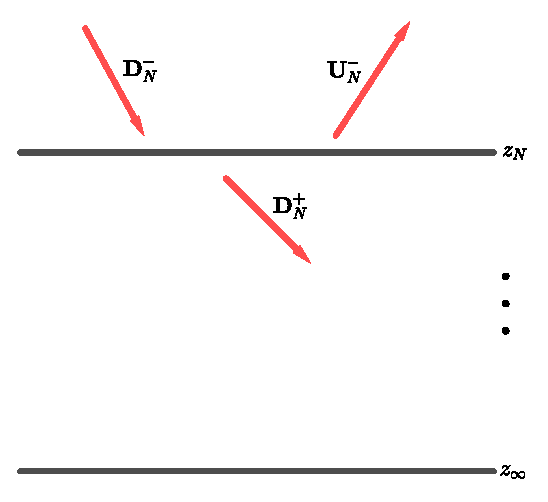
\includegraphics[scale=1]{ondas_em_zn}
\caption{\textit{Ondas ascendentes e descendentes na \'ultima interface.}}
\label{fig.ondas_em_zn}
\end{figure}

Substituindo a equa\c{c}\~ao \ref{eq.inversa_matriz_salto} na equa\c{c}\~ao anterior, temos
\begin{align*}
\begin{pmatrix}
\mathbf{U}_N^-\\
\mathbf{D}_N^-
\end{pmatrix}
&=
\begin{pmatrix}
J_{A,N}^\top&-J_{B,N}^\top\\
-J_{B,N}^\top&J_{A,N}^\top
\end{pmatrix}
\,
\begin{pmatrix}
0\\
\mathbf{D}_N^+
\end{pmatrix}\\\\
&=
\begin{pmatrix}
-J_{B,N}^\top \mathbf{D}_N^+\\
 J_{A,N}^\top \mathbf{D}_N^+
\end{pmatrix},
\end{align*}
ou seja,
\begin{align*}
\mathbf{U}_N^-&=-J_{B,N}^\top J_{A,N}^{-\top}\mathbf{D}_N^-\\
\mathbf{D}_N^+&=J_{A,N}^{-\top}\mathbf{D}_N^-.
\end{align*}
Assim, vemos que para computar uma onda refletida, ou seja, uma onda ascendente a partir de uma interface entre camadas, usamos uma \textit{matriz de reflex\~ao} que fica definida como
\begin{equation}\label{eq.reflexao_N}
\Gamma_N=-J_{B,N}^\top J_{A,N}^{-\top}.
\end{equation} 
Analogamente, vemos que para computar uma onda transmitida, ou seja, uma onda descendente a partir de uma interface entre camadas, usamos uma \textit{matriz de transmiss\~ao} que fica definida como
\begin{equation}\label{eq.transmissao_N}
T_N=J_{A,N}^{-\top}.
\end{equation} 

\subsection{Reflex\~ao e Transmiss\~ao numa Interface Qualquer}
Definimos a espessura de uma camada, a partir da interface superior, como
\begin{equation}
\Delta\,z_m=z_{m+1}-z_m,\qquad m=1,2,...,N-1,
\end{equation}
e temos que uma onda se propagando da interface na profundidade $z_m$ at\'e a interface em $z_{m+1}$ percorre uma profundidade total $\Delta\,z_m$. O valor dessa onda no fim da trajet\'oria, quando $z=z_{m+1}$, \'e aproximadamente igual a $\mathbf{\Psi}^-_{m+1}$, conforme a figura \ref{fig.N_interfaces}. Assim, usando a solu\c{c}\~ao \ref{eq.solucao_psi} podemos escrever
\begin{equation}\label{eq.solucao_delta_zm}
\mathbf{\Psi}^-_{m+1}=e^{-i\,\omega\tilde{\Lambda}_m\Delta\,z_m}\mathbf{\Psi}^+_m.
\end{equation}

\begin{figure}
\centering
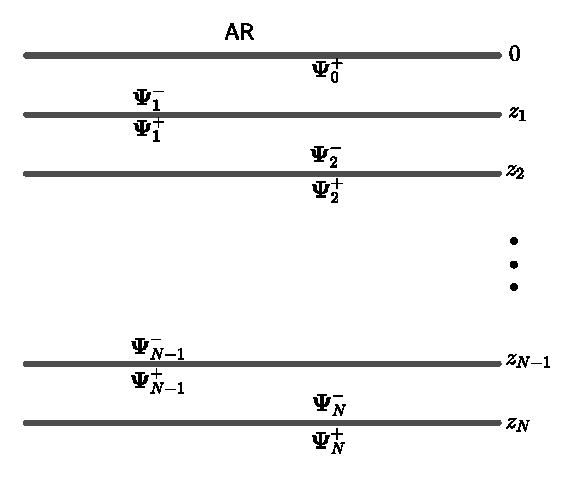
\includegraphics[scale=1]{n_interfaces}
\caption{\textit{Visualizacao de $N$ interfaces em subsuperficie e a notacao das ondas nas proximadades de cada interface.}}
\label{fig.N_interfaces}
\end{figure}

Sabendo que essa onda se propagando na camada abaixo da interface em $z_m$ veio da camada anterior, podemos usar a matriz de salto na equa\c{c}\~ao \ref{eq.psi_matriz_salto} e escrever
\begin{align}\label{eq.salto_m}
\mathbf{\Psi}^+_{m}&=J_m\,\mathbf{\Psi}^-_m.\\
\end{align}
Substituindo a equa\c{c}\~ao \ref{eq.salto_m} na equa\c{c}\~ao \ref{eq.solucao_delta_zm}, temos
\begin{align*}
\mathbf{\Psi}^-_{m+1}&=e^{-i\,\omega\tilde{\Lambda}_m\Delta\,z_m}\mathbf{\Psi}^+_m\\
\mathbf{\Psi}^-_{m+1}&=e^{-i\,\omega\tilde{\Lambda}_m\Delta\,z_m}J_m\,\mathbf{\Psi}^-_m\\
\mathbf{\Psi}^-_m&=J^{-1}_me^{i\,\omega\tilde{\Lambda}_m\Delta\,z_m}\mathbf{\Psi}^-_{m+1}
\end{align*}
Substituindo a equa\c{c}\~ao \ref{eq.definicao_psi} e a equa\c{c}\~ao \ref{eq.inversa_matriz_salto}, temos
\begin{align}\label{eq.refle_trans_1}
\mathbf{U}_m^-&=J^\top_{A,m}e^{i\,\omega\Lambda_m\Delta\,z_m}\mathbf{U}^-_{m+1}-J^\top_{B,m}e^{-i\,\omega\Lambda_m\Delta\,z_m}\mathbf{D}^-_{m+1}\\\nonumber\\\label{eq.refle_trans_2}
\mathbf{D}_m^-&=-J^\top_{B,m}e^{i\,\omega\Lambda_m\Delta\,z_m}\mathbf{U}^-_{m+1}+J^\top_{A,m}e^{-i\,\omega\Lambda_m\Delta\,z_m}\mathbf{D}^-_{m+1}.
\end{align}
Assim como definimos matriz de reflex\~ao para a \'ultima interface em $z_N$, podemos definir a matriz de reflex\~ao para uma interface qualquer, ou seja,
\begin{equation}\label{eq.reflexao_m+1}
\mathbf{U}^-_{m+1}=\Gamma_{m+1}\mathbf{D}^-_{m+1}.
\end{equation}
Substituindo a equa\c{c}\~ao \ref{eq.reflexao_m+1} na equa\c{c}\~ao \ref{eq.refle_trans_1} e na equa\c{c}\~ao \ref{eq.refle_trans_2}, temos
\begin{align}\label{eq.refle_trans_3}
\mathbf{U}_m^-&=(J^\top_{A,m}e^{i\,\omega\Lambda_m\Delta\,z_m}\Gamma_{m+1}-J^\top_{B,m}e^{-i\,\omega\Lambda_m\Delta\,z_m})\mathbf{D}^-_{m+1}\\\nonumber\\\label{eq.refle_trans_4}
\mathbf{D}_m^-&=(-J^\top_{B,m}e^{i\,\omega\Lambda_m\Delta\,z_m}\Gamma_{m+1}+J^\top_{A,m}e^{-i\,\omega\Lambda_m\Delta\,z_m})\mathbf{D}^-_{m+1}\,.
\end{align}
Substituindo a equa\c{c}\~ao \ref{eq.refle_trans_4} na equa\c{c}\~ao \ref{eq.refle_trans_3}, temos
\begin{align*}
\mathbf{U}_m^-&=(J^\top_{A,m}e^{i\,\omega\Lambda_m\Delta\,z_m}\Gamma_{m+1}-J^\top_{B,m}e^{-i\,\omega\Lambda_m\Delta\,z_m})\\
&\,\,\cdot\,\,(-J^\top_{B,m}e^{i\,\omega\Lambda_m\Delta\,z_m}\Gamma_{m+1}+J^\top_{A,m}e^{-i\,\omega\Lambda_m\Delta\,z_m})^{-1}\mathbf{D}_m^-\,,
\end{align*}
de onde podemos concluir que a matriz de reflex\~ao em uma interface em $z_m$ qualquer \'e dada por
\begin{align*}
\Gamma_{m}&=(J^\top_{A,m}e^{i\,\omega\Lambda_m\Delta\,z_m}\Gamma_{m+1}-J^\top_{B,m}e^{-i\,\omega\Lambda_m\Delta\,z_m})\\
&\,\,\cdot\,\,(-J^\top_{B,m}e^{i\,\omega\Lambda_m\Delta\,z_m}\Gamma_{m+1}+J^\top_{A,m}e^{-i\,\omega\Lambda_m\Delta\,z_m})^{-1},
\end{align*}
ou
\begin{align}\nonumber
\Gamma_{m}&=(J^\top_{A,m}e^{i\,\omega\Lambda_m\Delta\,z_m}\Gamma_{m+1}e^{i\,\omega\Lambda_m\Delta\,z_m}-J^\top_{B,m})\\\label{eq.matriz_reflexao_m}
&\,\,\cdot\,\,(-J^\top_{B,m}e^{i\,\omega\Lambda_m\Delta\,z_m}\Gamma_{m+1}e^{i\,\omega\Lambda_m\Delta\,z_m}+J^\top_{A,m})^{-1}.
\end{align}
Quando uma onda atinge uma interface, alem da possibilidade de reflexao ha tambem a possibilidade de trasmissao da onda para a camada inferior. De maneira analoga ao desenvolvido para reflexao de ondas, podemos deduzir a matriz para a transmissao de ondas em uma interface qualquer, que eh dada por
\begin{equation}\label{eq.matriz_transmissao_m}
T_m=T_{m+1}e^{i\,\omega\,\Lambda\Delta\,z_m}(-J^\top_{B,m}e^{i\,\omega\Lambda_m\Delta\,z_m}\Gamma_{m+1}e^{i\,\omega\Lambda_m\Delta\,z_m}+J^\top_{A,m})^{-1}.
\end{equation}
A validade das equacoes \ref{eq.matriz_reflexao_m} e \ref{eq.matriz_transmissao_m} para qualquer interface pode ser demonstrada por inducao sobre $m$, e todas as matrizes de reflexao e transmissao podem ser computadas por recurssao partindo das equacoes \ref{eq.reflexao_N} e \ref{eq.transmissao_N}.





mesclado
% %\chapter{Solu\c{c}\~ao na Presen\c{c}a de Fonte}\label{sec.presenca_fonte}
Em porspec\c{c}\~ao de petr\'oleo s\~ao utilizadas alguns tipos de fontes de ondas, atrav\'es das quais se faz um mapeamento das caracter\'isticas das camadas de subsuperf\'icie. Esses tipos de fontes podem ser uma queda de peso, um caminh\~ao \textit{vibroseis}, explosivos e canh\~ao de ar, esta \'ultima fonte utilizada em prospec\c{c}\~ao mar\'itima. Sendo assim, vamos desenvolver uma solu\c{c}\~ao para o nosso problema considerando agora a presen\c{c}a de uma fonte.

Considere ainda a equa\c{c}\~ao \ref{eq.matricial} com o sobrescrito $m$ omitido. Uma fonte $\mathbf{S}$ localizada numa profundidade $z_s$ pode ser representada na forma
\begin{equation}\label{eq.fonte_geral}
\mathbf{S}=\mathbf{S}_0\delta(z-z_s)+\mathbf{S}_1\delta^\prime(z-z_s),
\end{equation}
onde $\mathbf{S}_0$ e $\mathbf{S}_1$ n\~ao dependem da profundidade e $\delta$ \'e a fun\c{c}ao \textit{Delta de Dirac}. Fontes que s\~ao distribu\'idas ao longo da profundidade podem, geralmente, ser sintetizadas por superposi\c{c}\~ao de fontes do tipo $\mathbf{S}_0$ e $\mathbf{S}_1$. 

Uma solu\c{c}\~ao por ser escrita como a combina\c{c}\~ao de uma solu\c{c}\~ao inicial sofrendo a a\c{c}\~ao de alguma fonte, ou seja,
\begin{equation}\label{eq.solucao_inicial_fonte}
\mathbf{\Phi}=\mathbf{\Phi}_0+\mathbf{S}_1\delta(z-z_s).
\end{equation} 
Substituindo a equa\c{c}\~ao \ref{eq.solucao_inicial_fonte} e a equa\c{c}\~ao \ref{eq.fonte_geral} na equa\c{c}\~ao \ref{eq.matricial}, temos
\begin{equation}\label{eq.matricial_fonte}
\frac{d\,\mathbf{\Phi}_0}{d\,z}=-i\,\omega\,M\,\mathbf{\Phi}_0+\left[\mathbf{S}_0-i\,\omega\,M\,\mathbf{S}_1\right]\,\delta(z-z_s),
\end{equation}
e por simplicidade, vamos escrever
\begin{equation}\label{eq.fonte_simplificada}
i\,\omega\,M\,\mathbf{S}_1-\mathbf{S}_0=
\begin{pmatrix}
\mathbf{S}_A\\
\mathbf{S}_B
\end{pmatrix}.
\end{equation}
Considerando a exist\^encia de uma interface imagin\'aria na profundidade $z_s$ da fonte, podemos determinar as condi\c{c}\~oes de salto no local da fonte da mesma forma que estudamos as condi\c{c}\~oes de salto nas interfaces que separam as camadas. Assim, integrando a equa\c{c}\~ao \ref{eq.matricial_fonte} no intervalo que come\c{c}a imediatamente acima da interface imagin\'aria da fonte $z_s^-$, e termina imediatamente abaixo da interface imagin\'aria da fonte em $z_s^+$, e substituindo a equa\c{c}\~ao \ref{eq.fonte_simplificada}, temos como solu\c{c}\~ao
\begin{equation*}
\mathbf{\Phi}_0(z_s^-)=\mathbf{\Phi}_0(z_s^+)+
\begin{pmatrix}
\mathbf{S}_A\\
\mathbf{S}_B
\end{pmatrix}.
\end{equation*}
Substituindo a equa\c{c}\~ao \ref{eq.solucao_inicial_fonte} e considerando as caracter\'isticas da fun\c{c}\~ao Delta de Dirac, temos a seguinte condi\c{c}\~ao de salto na profundidade da fonte
\begin{equation}\label{eq.salto_zs}
\mathbf{\Phi}(z_s^-)=\mathbf{\Phi}(z_s^+)+
\begin{pmatrix}
\mathbf{S}_A\\
\mathbf{S}_B
\end{pmatrix}.
\end{equation}

Vamos agora inserir uma interface imagin\'aria imediatamente abaixo da fonte, em $z=z_s^+$ e utilizar os m\'etodos do cap\'itulo \ref{sec.ausencia_fonte} para computar a matriz de reflex\~ao $\Gamma_s\equiv\Gamma(z_s^+)$ a partir do topo desta camada. J\'a que a interface em $z_s^+$ eh fict\'icia, as propriedades do meio s\~ao iguais acima e abaixo dessa interface, assim temos que $L_2^+=L_2^-$ e $L_1^+=L_1^-$. Substituindo essas identidades nas equa\c{c}\~oes \ref{eq.j_a} e \ref{eq.j_b}, temos
\begin{align}\label{eq.j_a_ficticia}
J_A&=\frac{1}{2}\left[(L_2)^\top L_1+(L_1)^\top L_2\right]\\\label{eq.j_b_ficticia}
J_B&=\frac{1}{2}\left[(L_2)^\top L_1-(L_1)^\top L_2\right].
\end{align}
Pela diagonaliza\c{c}\~ao de Ursin apresentada nas subse\c{c}\~oes \ref{sec.diagonalizacao_1}-\ref{sec.diagonalizacao_4}, conclu\'imos que 
\begin{align*}
L_1^\top&=L_2^{-1}\\
L_2^\top&=L_1^{-1},
\end{align*}
e substituindo as equa\c{c}\~oes acima nas equa\c{c}\~oes \ref{eq.j_a_ficticia} e \ref{eq.j_b_ficticia}, obtemos que
\begin{align*}
J_A&=I\\
J_B&=0.
\end{align*}
Desta forma, a onda ascendente $\mathbf{U}(z_s^+)$ e a onda descendente $\mathbf{D}(z_s^+)$ a partir da interface em $z_s^+$ podem ser introduzidas na equa\c{c}\~ao \ref{eq.definicao_psi} para obtermos
\begin{equation*}
\mathbf{\Psi}(z_s^+)=
\begin{pmatrix}
\mathbf{U}(z_s^+)\\
\mathbf{D}(z_s^+)
\end{pmatrix}.
\end{equation*}
Substituindo a equa\c{c}\~ao \ref{eq.reflexao_m+1} na equa\c{c}\~ao acima, temos
\begin{equation}\label{eq.Psi_descendente}
\mathbf{\Psi}(z_s^+)=
\begin{pmatrix}
\Gamma_s\mathbf{D}(z_s^+)\\
\mathbf{D}(z_s^+)
\end{pmatrix},
\end{equation}
pois as ondas est\~ao numa mesma camada e da\'i usamos que
\begin{align*}
\mathbf{U}^-(z_s^+)&=\mathbf{U}(z_s^+)\\
\mathbf{D}^-(z_s^+)&=\mathbf{D}(z_s^+).
\end{align*}
Multiplicando a equa\c{c}\~ao \ref{eq.salto_zs} por $L^{-1}$ e substituindo a equa\c{c}\~ao \ref{eq.Phi}, obtemos
\begin{equation}\label{eq.Psi_salto_zs}
\mathbf{\Psi}(z_s^-)=\mathbf{\Psi}(z_s^+)+L^{-1}
\begin{pmatrix}
\mathbf{S}_A\\
\mathbf{S}_B
\end{pmatrix}.
\end{equation}
Generalizando os desenvolvimentos apresentados nas subse\c{c}\~oes \ref{sec.diagonalizacao_1}-\ref{sec.diagonalizacao_4}, podemos escrever 
\begin{equation*}
L^{-1}=\frac{1}{\sqrt{2}}
\begin{pmatrix}
L_2^\top&L_1^\top\\
L_2^\top&-L_1^\top
\end{pmatrix},
\end{equation*}
e substituindo esta express\~ao para $L^{-1}$ juntamente com a equa\c{c}\~ao \ref{eq.Psi_descendente} na equa\c{c}\~ao \ref{eq.Psi_salto_zs}, temos
\begin{equation}\label{eq.solucao_phi_zs-}
\mathbf{\Psi}(z_s^-)=
\begin{pmatrix}
\Gamma_s\mathbf{D}(z_s^+)\\
\mathbf{D}(z_s^+)
\end{pmatrix}
+
\frac{1}{\sqrt{2}}\,
\begin{pmatrix}
L_2^\top\mathbf{S}_A+L_1^\top\mathbf{S}_B\\
L_2^\top\mathbf{S}_A-L_1^\top\mathbf{S}_B
\end{pmatrix}.
\end{equation}
Admitindo que a fonte esteja no interior da primeira camada, ou seja, $0<z_s<z_1$, a solu\c{c}\~ao dada pela equa\c{c}\~ao \ref{eq.solucao_phi_zs-} \'e propagada para cima a partir de $z_s^-$ usando a equa\c{c}\~ao \ref{eq.solucao_psi}, e o salto atrav\'es das interfaces entre camadas \'e dado pela equa\c{c}\~ao \ref{eq.psi_matriz_salto} at\'e que a onda atinja a interface terra/ar em $z=0^+$. Assim,
\begin{equation*}
\mathbf{\Psi}(0^+)=e^{-i\,\omega\,\tilde{\mathbf{\Lambda}}\,(0^+-z_s^-)}\,\mathbf{\Psi}(z_s^-),
\end{equation*}
e podemos usar as $n$ condi\c{c}\~oes de fronteira em $z=0$ para determinarmos as $n$ inc\'ognitas de $\mathbf{D}_s$. Os demais termos da solu\c{c}\~ao s\~ao conhecidos. A diferen\c{c}a $z_s^--0^+$ corresponde \`a profundidade da fonte, assim a solu\c{c}\~ao anterior pode ser reescrita como
\begin{align*}
\mathbf{\Psi}(0^+)&=e^{-i\,\omega\,\tilde{\mathbf{\Lambda}}\,(-z_s)}\,\mathbf{\Psi}(z_s^-)\\\\
\mathbf{\Psi}(0^+)&=
\begin{pmatrix}
e^{i\,\omega\,\mathbf{\Lambda}\,z_s}&\mathbf{0}\\
\mathbf{0}&e^{-i\,\omega\,\mathbf{\Lambda}\,z_s}
\end{pmatrix}
\mathbf{\Psi}(z_s^-).
\end{align*}
Substituindo a equa\c{c}\~ao \ref{eq.solucao_phi_zs-} na equa\c{c}\~ao acima, temos
\begin{equation}\label{eq.Psi_zero+}
\mathbf{\Psi}(0^+)=
\begin{pmatrix}
e^{i\,\omega\,\mathbf{\Lambda}\,z_s}\,\Gamma_s\mathbf{D}(z_s^+)\\
e^{-i\,\omega\,\mathbf{\Lambda}\,z_s}\,\mathbf{D}(z_s^+)
\end{pmatrix}
+
\frac{1}{\sqrt{2}}\,
\begin{pmatrix}
e^{i\,\omega\,\mathbf{\Lambda}\,z_s}\,(L_2^\top\mathbf{S}_A+L_1^\top\mathbf{S}_B)\\
e^{-i\,\omega\,\mathbf{\Lambda}\,z_s}\,(L_2^\top\mathbf{S}_A-L_1^\top\mathbf{S}_B)
\end{pmatrix}.
\end{equation}

TALVEZ SEJA INTERESSANTE COLOCAR A PARTE SEGUINTE NO CAPITULO ONDE SE DESENVOLVE AS EQUACOES MAIS PARTICULARES.

Para an\'alises futuras ser\'a interessante escrever a solu\c{c}\~ao na superf\'icie como
\begin{equation}\label{eq.Phi_G_AB}
\mathbf{\Phi}(0^+)=
\begin{pmatrix}
G_A\mathbf{\Phi}_g\\
G_B\mathbf{\Phi}_g
\end{pmatrix},
\end{equation}
onde as matrizes $G_A$ $G_B$ s\~ao de dimens\~ao $n\times n$ e $\mathbf{\Phi}_g$ \'e um vetor de dimens\~ao $n$ formado por inc\'ognitas em $z=0$.
Considerando o sistema \ref{eq.matricial_1}, temos
\begin{equation*}
\mathbf{\Phi}^{(1)}=
\begin{pmatrix}
\tilde{E}_1\\
\tilde{H}_2
\end{pmatrix}
\end{equation*}
e sua condi\c{c}\~ao de fronteira, quando $z=0$ \'e dada pela equa\c{c}\~ao \ref{eq.cond_fron_1}, 
\begin{equation*}
\tilde{H}_2=-\frac{\epsilon_0}{q_0}\tilde{E}_1.
\end{equation*}
Substituindo esta condi\c{c}\~ao em $\mathbf{\Phi}^{(1)}$, temos
\begin{equation*}
\mathbf{\Phi}^{(1)}=
\begin{pmatrix}
\tilde{E}_1\\\\
-\frac{\epsilon_0}{q_0}\tilde{E}_1
\end{pmatrix}_{z=0^+}.
\end{equation*}
Colocando a equa\c{c}\~ao acima no formato da equa\c{c}\~ao \ref{eq.Phi_G_AB}, temos que
\begin{equation*}
\mathbf{\Phi}_g^{(1)}=\tilde{E}_1,
\end{equation*}
\begin{equation*}
G_A^{(1)}=1\qquad\text{e}\qquad G_B^{(1)}=-\frac{\epsilon_0}{q_0}.
\end{equation*}
De maneira an\'aloga, vamos escrever as solu\c{c}\~oes dos tr\^es sistemas restantes na forma dada pela equa\c{c}\~ao \ref{eq.Phi_G_AB}. Substituindo a condi\c{c}\~ao de contorno \ref{eq.cond_fron_2} no sistema \ref{eq.matricial_2}, $\mathbf{\Phi}^{(2)}$ \'e dado por
\begin{equation*}
\mathbf{\Phi}^{(2)}=
\begin{pmatrix}
\tilde{E}_2\\\\
-\frac{q_0}{\mu_0}\tilde{E}_2
\end{pmatrix}_{z=0^+}
\end{equation*}
e temos
\begin{equation*}
\mathbf{\Phi}_g^{(2)}=\tilde{E}_2,
\end{equation*}
\begin{equation*}
G_A^{(2)}=1\qquad\text{e}\qquad G_B^{(2)}=-\frac{q_0}{\mu_0}.
\end{equation*}
Substituindo a condi\c{c}\~ao de contorno \ref{eq.cond_fron_3} no sistema \ref{eq.matricial_3}, $\mathbf{\Phi}^{(3)}$ \'e dado por
\begin{equation*}
\mathbf{\Phi}^{(3)}=
\begin{pmatrix}
\dot{\tilde{u}}_3\\
0\\
0\\
\dot{\tilde{u}}_1
\end{pmatrix}_{z=0^+}
\end{equation*}
e temos,
\begin{equation*}
\mathbf{\Phi}_g^{(3)}=
\begin{pmatrix}
\dot{\tilde{u}}_3\\
\dot{\tilde{u}}_1
\end{pmatrix},
\end{equation*}
\begin{equation*}
G_A^{(3)}=
\begin{pmatrix}
1&0\\
0&0
\end{pmatrix}
\qquad\text{e}\qquad G_B^{(3)}=
\begin{pmatrix}
0&0\\
0&1
\end{pmatrix}.
\end{equation*}

Substituindo a condi\c{c}\~ao de contorno \ref{eq.cond_fron_4} no sistema \ref{eq.matricial_4}, $\mathbf{\Phi}^{(4)}$ \'e dado por
\begin{equation*}
\mathbf{\Phi}^{(4)}=
\begin{pmatrix}
\dot{\tilde{u}}_2\\
0
\end{pmatrix}_{z=0^+}
\end{equation*}
e temos,
\begin{equation*}
\mathbf{\Phi}_g^{(4)}=\dot{\tilde{u}}_2,
\end{equation*}
\begin{equation*}
G_A^{(4)}=1\qquad\text{e}\qquad G_B^{(4)}=0.
\end{equation*}

De acordo com a equa\c{c}\~ao \ref{eq.Phi}, podemos escrever
\begin{equation*}
\mathbf{\Phi}(0^+)=L\,\mathbf{\Psi}(0^+),
\end{equation*}
e substituindo as equa\c{c}\~oes \ref{eq.Psi_zero+}, \ref{eq.Phi_G_AB} e \ref{eq.matriz_L} na equa\c{c}\~ao acima, temos
\begin{align}\label{eq.GA_Phi}
G_A\mathbf{\Phi}_g&=\frac{1}{\sqrt{2}}\,(L_1e^{i\,\omega\,\Lambda\,z_s}\Gamma_s\mathbf{D}_s+L_1e^{-i\,\omega\,\Lambda\,z_s}\mathbf{D}_s)\\\nonumber
&+\frac{1}{2}\,\left[L_1e^{i\,\omega\,\Lambda\,z_s}(L_2^\top\mathbf{S}_A+L_1^\top\mathbf{S}_B)+L_1e^{-i\,\omega\,\Lambda\,z_s}(L_2^\top\mathbf{S}_A-L_1^\top\mathbf{S}_B)\right]
\end{align}
e
\begin{align}\label{eq.GB_Phi}
G_B\mathbf{\Phi}_g&=\frac{1}{\sqrt{2}}\,(L_2e^{i\,\omega\,\Lambda\,z_s}\Gamma_s\mathbf{D}_s-L_2e^{-i\,\omega\,\Lambda\,z_s}\mathbf{D}_s)\\\nonumber
&+\frac{1}{2}\,\left[L_2e^{i\,\omega\,\Lambda\,z_s}(L_2^\top\mathbf{S}_A+L_1^\top\mathbf{S}_B)-L_2e^{-i\,\omega\,\Lambda\,z_s}(L_2^\top\mathbf{S}_A-L_1^\top\mathbf{S}_B)\right].
\end{align}
Pela diagonaliza\c{c}\~ao de Ursin podemos verificar que $L_1^\top=L_2^{-1}$, e multiplicando pela esquerda a equa\c{c}\~ao \ref{eq.GA_Phi} por $L_2^\top$ e multiplicando pela esquerda a equa\c{c}\~ao \ref{eq.GB_Phi} por $L_1^\top$, temos 
\begin{align}\label{eq.LGA_Phi}
L_2^{\top}G_A\mathbf{\Phi}_g&=\frac{1}{\sqrt{2}}\,(e^{i\,\omega\,\Lambda\,z_s}\Gamma_s\mathbf{D}_s+e^{-i\,\omega\,\Lambda\,z_s}\mathbf{D}_s)\\\nonumber
&+\frac{1}{2}\,\left[e^{i\,\omega\,\Lambda\,z_s}(L_2^\top\mathbf{S}_A+L_1^\top\mathbf{S}_B)+e^{-i\,\omega\,\Lambda\,z_s}(L_2^\top\mathbf{S}_A-L_1^\top\mathbf{S}_B)\right]
\end{align}
e
\begin{align}\label{eq.LGB_Phi}
L_1^\top G_B\mathbf{\Phi}_g&=\frac{1}{\sqrt{2}}\,(e^{i\,\omega\,\Lambda\,z_s}\Gamma_s\mathbf{D}_s-e^{-i\,\omega\,\Lambda\,z_s}\mathbf{D}_s)\\\nonumber
&+\frac{1}{2}\,\left[e^{i\,\omega\,\Lambda\,z_s}(L_2^\top\mathbf{S}_A+L_1^\top\mathbf{S}_B)-e^{-i\,\omega\,\Lambda\,z_s}(L_2^\top\mathbf{S}_A-L_1^\top\mathbf{S}_B)\right].
\end{align}
Subtraindo a equa\c{c}\~ao \ref{eq.LGB_Phi} da equa\c{c}\~ao \ref{eq.LGA_Phi}, temos
\begin{equation}\label{eq.pre_phi_g}
(L_2^{\top}G_A-L_1^\top G_B)\mathbf{\Phi}_g=\frac{2}{\sqrt{2}}\,e^{-i\,\omega\,\Lambda\,z_s}\mathbf{D}_s+e^{-i\,\omega\,\Lambda\,z_s}(L_2^\top\mathbf{S}_A-L_1^\top\mathbf{S}_B).
\end{equation}
Isolando $\mathbf{D}_s$ obtemos
\begin{equation*}
\mathbf{D}_s=\frac{1}{\sqrt{2}}\,e^{i\,\omega\,\Lambda\,z_s}(L_2^{\top}G_A-L_1^\top G_B)\,\mathbf{\Phi}_g-\frac{1}{\sqrt{2}}(L_2^\top\mathbf{S}_A-L_1^\top\mathbf{S}_B).
\end{equation*}
Ao multiplicar pela esquerda a equa\c{c}\~ao \ref{eq.pre_phi_g} por $e^{i\,\omega\,\Lambda\,z_s}\,\Gamma_se^{i\,\omega\,\Lambda\,z_s}$, temos
\begin{equation}\label{eq.pre_phi_g2}
e^{i\,\omega\,\Lambda\,z_s}\,\Gamma_se^{i\,\omega\,\Lambda\,z_s}(L_2^{\top}G_A-L_1^\top G_B)\mathbf{\Phi}_g=\frac{2}{\sqrt{2}}\,e^{i\,\omega\,\Lambda\,z_s}\,\Gamma_s\mathbf{D}_s+e^{i\,\omega\,\Lambda\,z_s}\,\Gamma_s(L_2^\top\mathbf{S}_A-L_1^\top\mathbf{S}_B),
\end{equation}
e somando as equa\c{c}\~oes \ref{eq.LGA_Phi} e \ref{eq.LGB_Phi}, temos
\begin{equation}\label{eq.pre_phi_g+}
(L_2^{\top}G_A+L_1^\top G_B)\mathbf{\Phi}_g=\frac{2}{\sqrt{2}}\,e^{i\,\omega\,\Lambda\,z_s}\Gamma_s\mathbf{D}_s+e^{i\,\omega\,\Lambda\,z_s}(L_2^\top\mathbf{S}_A+L_1^\top\mathbf{S}_B).
\end{equation}
Subtraindo a equa\c{c}\~ao \ref{eq.pre_phi_g+} da equa\c{c}\~ao \ref{eq.pre_phi_g2}, obtemos uma rela\c{c}\~ao para $\mathbf{\Phi}_g$, dada por 
\begin{align*}
\mathbf{\Phi}_g&=\left[e^{i\,\omega\,\Lambda\,z_s}\,\Gamma_se^{i\,\omega\,\Lambda\,z_s}(L_2^{\top}G_A-L_1^\top G_B)-(L_2^{\top}G_A+L_1^\top G_B)\right]^{-1}\\
&\,\,\cdot\,\,e^{i\,\omega\,\Lambda\,z_s}\left[\Gamma_s (L_2^\top\mathbf{S}_A-L_1^\top\mathbf{S}_B)-(L_2^\top\mathbf{S}_A+L_1^\top\mathbf{S}_B)\right].
\end{align*}
Em particular, quando a fonte est\'a imediatamente abaixo da superf\'icie livre, $z_s\approx0$, temos
\begin{equation*}
\mathbf{\Phi}_g=\left[(\Gamma_s-I)L_2^{\top}G_A-(\Gamma_s+I)L_1^\top G_B\right]^{-1}\left[(\Gamma_s-I)L_2^\top\mathbf{S}_A-(\Gamma_s+I)L_1^\top\mathbf{S}_B\right].
\end{equation*} 
Ap\'os obtermos $\mathbf{\Phi}_g$, \'e poss\'ivel determinarmos todas as condi\c{c}\~oes iniciais em $z=0$, $\mathbf{D}_s$ e $\mathbf{U}_s=\Gamma\,\mathbf{D}_s$. Em seguida, podemos obter a solu\c{c}\~ao imediatamente abaixo da fonte conforme a rela\c{c}\~ao \ref{eq.Psi_descendente}. Teoricamente, a partir de agora, a solu\c{c}\~ao pode ser computada em qualquer outra profundidade utilizando a propaga\c{c}\~ao atrav\'es das camadas de acordo com a rela\c{c}\~ao \ref{eq.solucao_psi} e o salto atrav\'es das camadas usando a rela\c{c}\~ao \ref{eq.psi_matriz_salto}. No entando, a propaga\c{c}\~ao de uma onda ascendente cont\'inua no sentido descendente \'e numericamente inst\'avel usando a equa\c{c}\~ao \ref{eq.solucao_psi}, pois as exponenciais complexas crescem ao inv\'es de diminuirem com a dist\^ancia. Assim, devemos obter $\mathbf{U}$ a partir de $\mathbf{D}$ usando $\Gamma_m$, ou fazer uso das matrizes de transmiss\~ao $T_m$.


mesclado

%\chapter{Escrevendo as EDP's como um Sistema de EDO's}
Neste capitulo vamos aplicar algumas tecnicas como rotacao do sistema de coordenadas e Transformadas Laterais de Fourier em EDP's para que as mesmas possam ser escritas como um sistema de EDO's.

\section{Sistema de EDP's do Efeito Magnetoel\'astico}

Segundo \cite{eringen_1963}, o acoplamento entre ondas eletromagn\'eticas e el\'asticas se propagando no subsolo caracteriza o efeito magnetoel\'astico, e esse acoplamento pode ser modelado matematicamente atrav\'es de um sistema de equa\c{c}\~oes diferencias parciais. Conforme minha monografia, podemos aplicar uma s\'erie de hip\'oteses que visam simplificar e linearizar essas EDP's de forma que as mesmas possam receber um tratamento matem\'atico adequado no sentido de se obter numericamente os valores dos campos eletromagn\'eticos e el\'asticos envolvidos no sistema. Desta forma, vamos utilizar o m\'etodo matricial encontrado em \cite{Ursin-1983} na solu\c{c}\~ao do seguinte sistema de EDP's da magnetoelasticidade
\begin{align}\label{eq.mag_ela_1}
\nabla\times\mathbf{{E}}&=i\,\omega\,\mu_0\mathbf{{H}}\\\nonumber\\\label{eq.mag_ela_2}
\nabla\times\mathbf{{H}}&=(\sigma-i\,\epsilon\,\omega)\,\mathbf{{E}}+\mathbf{{v}}\times\sigma\mu_0\mathbf{H}^0\\\nonumber\\\label{eq.mag_ela_3}
-i\,\omega\rho\,\mathbf{{v}}&=\nabla\cdot{\tau} + \mathbf{{F}}\\\nonumber\\\label{eq.mag_ela_4}
{\tau}&=\lambda\,\nabla\cdot\mathbf{{u}}\cdot\,I + G\,(\nabla\,\mathbf{{u}}+\nabla\mathbf{{u}}^\top)\\\nonumber\\\label{eq.mag_ela_5}
\nabla\cdot\mathbf{{H}}&=0.
\end{align}
Estas equa\c{c}\~oes est\~ao no dom\'inio da frequ\^encia $\omega$, a depend\^encia do tempo \'e dada por $\exp{-i\,\omega\,t}$ e 
\begin{itemize}
\item $\mathbf{{E}}$ \'e o campo el\'etrico,
\item $\mathbf{{B}}$ \'e o campo magn\'etico,
\item $\mathbf{{D}}$ \'e o campo de densidade de fluxo el\'etrico,
\item $\mathbf{{H}}$ \'e o campo magn\'etico auxiliar,
\item $\tau$ \'e o tensor de tens\~oes,
\item $\mathbf{{u}}$ \'e o deslocamento do meio,
\item $\mathbf{{v}}$ \'e a velocidade de deslocamento do meio,
\item $\mathbf{{F}}$ \'e uma for\c{c}a aplicada ao meio,
\item $\mathbf{H}^0$ \'e campo geomagn\'etico,
\item $i$ \'e um n\'umero complexo,
\item $\omega$ \'e a frequ\^encia temporal,
\item $\mu_0$ \'e a permeabilidade magn\'etica no v\'acuo,
\item $\sigma$ \'e a condutividade do meio,
\item $\epsilon$ \'e a permissividade el\'etrica do meio,
\item $\rho$ \'e a densidade do meio,
\item $\lambda$ e $G$ s\~ao par\^ametros de Lam\`e.
\end{itemize}
Vamos definir $\sigma^*=(\sigma-i\,\epsilon\,\omega)$. No subsolo, por conta do regime quasi-estacion\'ario, $(\sigma>>\epsilon\,\omega)$  e  temos $\sigma^*=\sigma$. No ar, a condutividade \'e zero e a permeabilidade el\'etrica \'e pr\'oxima a do v\'acuo $\epsilon_0$, assim temos $\sigma^*=-i\,\epsilon_0\omega$.

No formato matricial, a equacao \ref{eq.mag_ela_1} pode ser escrita como
\begin{equation*}
\begin{pmatrix}
\frac{\partial\,E_3}{\partial\,y}-\frac{\partial\,E_2}{\partial\,z}\\
\frac{\partial\,E_1}{\partial\,z}-\frac{\partial\,E_3}{\partial\,x}\\
\frac{\partial\,E_2}{\partial\,x}-\frac{\partial\,E_1}{\partial\,y}
\end{pmatrix}
=
i\,\omega\,\mu_0\,
\begin{pmatrix}
H_1\\
H_2\\
H_3
\end{pmatrix}.
\end{equation*}
Aplicando as transformadas laterais de Fourier, dada em \ref{eq.trans_fourier_1}, temos
\begin{empheq}[left=\empheqlbrace]{align*}
-i\,k_y\widehat{E}_3-\frac{\partial\,\widehat{E}_2}{\partial\,z}&=i\,\omega\,\mu_0\widehat{H}_1\\
\frac{\partial\,\widehat{E}_1}{\partial\,z}+i\,k_x\widehat{E}_3&=i\,\omega\,\mu_0\widehat{H}_2\\
-i\,k_x\widehat{E}_2+i\,k_y\widehat{E}_1&=i\,\omega\,\mu_0\widehat{H}_3.
\end{empheq} 
Rotacionando o sistema de forma que a primeira coordenada esteja orientada no sentido do vetor de onda horizontal, usando o operador dado pela equacao \ref{eq.operador_rotacao}, e fazendo as simplificacoes, temos
\begin{empheq}[left=\empheqlbrace]{align*}
\frac{\partial\,\tilde{E}_2}{\partial\,z}&=-i\,\omega\,\mu_0\tilde{H}_1\\
\frac{\partial\,\tilde{E}_1}{\partial\,z}&=i\,\omega\,\mu_0\tilde{H}_2-i\,k\tilde{E}_3\\
\tilde{E}_2&=-\frac{\omega\,\mu_0}{k}\tilde{H}_3.
\end{empheq}

Observando que $\mathbf{v}=-i\,\omega\mathbf{u}$ depois de aplicada a transformada de Fourier no tempo, a equacao \ref{eq.mag_ela_2} pode ser escrita como
\begin{equation*}
\begin{pmatrix}
\frac{\partial\,H_3}{\partial\,y}-\frac{\partial\,H_2}{\partial\,z}\\
\frac{\partial\,H_1}{\partial\,z}-\frac{\partial\,H_3}{\partial\,x}\\
\frac{\partial\,H_2}{\partial\,x}-\frac{\partial\,H_1}{\partial\,y}
\end{pmatrix}
=
(\sigma-i\,\epsilon\,\omega)\,
\begin{pmatrix}
E_1\\
E_2\\
E_3
\end{pmatrix}
-i\,\omega\,
\begin{pmatrix}
u_2H_3^0-u_3H_2^0\\
u_3H_1^0-u_1H_3^0\\
u_1H_2^0-u_2H_1^0
\end{pmatrix}.
\end{equation*}
Aplicando as transformadas laterais de Fourier conforme a equacao \ref{eq.trans_fourier_1}, temos
\begin{empheq}[left=\empheqlbrace]{align*}
-i\,k_y\widehat{H}_3-\frac{\partial\,\widehat{H}_2}{\partial\,z}&=(\sigma-i\,\epsilon\,\omega)\,\widehat{E}_1-i\,\omega(u_2H_3^0-u_3H_2^0)\\
\frac{\partial\,\widehat{H}_1}{\partial\,z}+i\,k_x\widehat{H}_3&=(\sigma-i\,\epsilon\,\omega)\,\widehat{E}_2-i\,\omega(u_3H_1^0-u_1H_3)\\
-i\,k_x\widehat{H}_2+i\,k_y\widehat{H}_1&=(\sigma-i\,\epsilon\,\omega)\,\widehat{E}_3-i\,\omega(u_1H_2^0-u_2H_1^0).
\end{empheq}
Rotacionando o sistema usando o operador dado pela equacao \ref{eq.operador_rotacao}, e fazendo as simplificacoes, temos
\begin{empheq}[left=\empheqlbrace]{align*}
\frac{\partial\,\tilde{H}_2}{\partial\,z}&=-(\sigma-i\,\epsilon\,\omega)\,\tilde{E}_1+i\,\omega\,\tilde{H}_3^0\tilde{u}_2-i\,\omega\,\tilde{H}_2^0\tilde{u}_3\\
\frac{\partial\,\tilde{H}_1}{\partial\,z}&=(\sigma-i\,\epsilon\,\omega)\,\tilde{E}_2-i\,\omega\,k\,\tilde{H}_3-i\,\omega\,\tilde{H}_1^0\tilde{u}_3+i\,\omega\,\tilde{H}_3^0\tilde{u}_1\\
\tilde{H}_2&=-\frac{(\sigma-i\,\epsilon\,\omega)}{i\,k}\tilde{E}_3+\frac{\omega}{k}  \tilde{H}_2^0\tilde{u}_1-\frac{\omega}{k}\tilde{H}_1^0\tilde{u}_2.
\end{empheq}

A equacao \ref{eq.mag_ela_3} pode ser reescrita como

\begin{empheq}[left=\empheqlbrace]{align*}
-\omega^2\rho\,u_1&=\frac{\partial \tau_{11}}{\partial\,x}+\frac{\partial \tau_{12}}{\partial\,y}+\frac{\partial \tau_{13}}{\partial\,z}+F_1\\
-\omega^2\rho\,u_2&=\frac{\partial \tau_{21}}{\partial\,x}+\frac{\partial \tau_{22}}{\partial\,y}+\frac{\partial \tau_{23}}{\partial\,z}+F_2\\
-\omega^2\rho\,u_3&=\frac{\partial \tau_{31}}{\partial\,x}+\frac{\partial \tau_{32}}{\partial\,y}+\frac{\partial \tau_{33}}{\partial\,z}+F_3
\end{empheq}
Aplicando as transformadas laterais de Fourier, temos
\begin{empheq}[left=\empheqlbrace]{align*}
-\omega^2\rho\,\widehat{u}_1&=-i\,k_x\widehat{\tau}_{11}-i\,k_y\widehat{\tau}_{12}+\frac{\partial\widehat{\tau}_{13}}{\partial\,z}+\widehat{F}_1\\
-\omega^2\rho\,\widehat{u}_2&=-i\,k_x\widehat{\tau}_{21}-i\,k_y\widehat{\tau}_{22}+\frac{\partial\widehat{\tau}_{23}}{\partial\,z}+\widehat{F}_2\\
-\omega^2\rho\,\widehat{u}_3&=-i\,k_x\widehat{\tau}_{31}-i\,k_y\widehat{\tau}_{32}+\frac{\partial\widehat{\tau}_{33}}{\partial\,z}+\widehat{F}_3.
\end{empheq}
Aplicando a rotacao e simplificando as equacoes, temos
\begin{empheq}[left=\empheqlbrace]{align*}
-\omega^2\rho\,\tilde{u}_1&=-i\,k\tilde{\tau}_{11}+\frac{\partial\tilde{\tau}_{13}}{\partial\,z}+\tilde{F}_1\\
-\omega^2\rho\,\tilde{u}_2&=-i\,k\tilde{\tau}_{12}+\frac{\partial\tilde{\tau}_{23}}{\partial\,z}+\tilde{F}_2\\
-\omega^2\rho\,\tilde{u}_3&=-i\,k\tilde{\tau}_{13}+\frac{\partial\tilde{\tau}_{33}}{\partial\,z}+\tilde{F}_3.
\end{empheq}


%\chapter{Condi\c{c}\~oes de Contorno do Efeito Magneto-El\'astico e o Espa\c{c}o Original}

Como estamos assumindo que as propriedades materiais n\~ao se alteram no interior de cada camada da subsuperf\'icie, temos que a matriz $M^{(m)}$ \'e constante para cada camada. Essas propriedades materiais se alteram descontinuamente conforme $z$ varia de uma camada para outra atrav\'es da interface de contato entre as camadas. Nessas interfaces vamos aplicar as condi\c{c}\~oes de interface encontradas em \cite{pride_94}, onde o vetor $\mathbf{u}$, as componentes normais de $\tau$ e as componentes  tangenciais de $\mathbf{E}$ e $\mathbf{H}$ s\~ao cont\'inuas. Assim, constatamos que os vetores $\mathbf{\Phi}^{(m)}$ s\~ao cont\'inuos atrav\'es das interfaces entre as camadas.

\section{Condi\c{c}\~oes de Contorno}
Resta estabelecer condi\c{c}\~oes de contorno para os sistemas \ref{eq.matricial_1}-\ref{eq.matricial_4} no contato ar/superf\'icie, ou seja, em $z=0$. Aplicando ainda as condi\c{c}\~oes de interface encontradas em \cite{pride_94}, temos que a condi\c{c}\~ao de contorno para o sistema \ref{eq.matricial_1} \'e
\begin{equation}\label{eq.cond_fron_1}
\tilde{H}_2=-\frac{\epsilon_0}{q_0}\tilde{E}_1,
\end{equation}
onde $q_0$ \'e a vagarosidade vertical dada por \ref{eq.vagarosidade_vertical}. Esta \'e a rela\c{c}\~ao para uma onda eletromagn\'etica ascendente, e foi deduzida do fato de que n\~ao h\'a ondas eletromagn\'eticas descendentes no ar, pois todas a fontes est\~ao na subsuperf\'icie.
Para o sistema \ref{eq.matricial_2}, a condi\c{c}\~ao de contorno \'e
\begin{equation}\label{eq.cond_fron_2}
\tilde{H}_1=\frac{q_0}{\mu_0}\tilde{E}_2,
\end{equation}
onde esta rela\c{c}\~ao tamb\'em foi deduzida do fato de que h\'a apenas ondas eletromagn\'eticas ascendentes no ar.
Para o sistema \ref{eq.matricial_3}, as condi\c{c}\~oes de contorno s\~ao
\begin{equation}\label{eq.cond_fron_3}
\tilde{\tau}_{13}=\tilde{\tau}_{33}=0.
\end{equation}
E para o sistema \ref{eq.matricial_4}, a condi\c{c}\~ao de contorno \'e
\begin{equation}\label{eq.cond_fron_4}
\tilde{\tau}_{23}=0.
\end{equation}
Observe que para cada um dos sistemas, precisaremos de condi\c{c}\~oes de contorno adicionais para especificar uma solu\c{c}\~ao. Essas condi\c{c}\~oes surgir\~ao, por ocasi\~ao da aplica\c{c}\~ao nas equa\c{c}\~oes da magneto-elasticidade, do fato de que n\~ao h\'a ondas ascendentes em $z\rightarrow\infty$, como pudemos observar na subse\c{c}\~ao \ref{sec.ausencia_fonte} e na figura \ref{fig.ondas_em_zn}.

Essas condi\c{c}\~oes de contorno s\~ao utilizadas nas equa\c{c}\~oes da magneto-elasticidade mas podem desde j\'a serem inseridas na solu\c{c}\~ao gen\'erica apresentada na subse\c{c}\~ao \ref{sec.presenca_fonte}, como foi desenvolvido por v\'arios autores como \cite{White_Zhou_2006}, \cite{Azeredo_2013}, \cite{miranda_2016} e \cite{oliveira_2018}. Tal abordagem \'e interessante por facilitar an\'alises futuras, assim, vamos escrever a solu\c{c}\~ao na superf\'icie como
\begin{equation}\label{eq.Phi_G_AB}
\mathbf{\Phi}(0^+)=
\begin{pmatrix}
G_A\mathbf{\Phi}_g\\
G_B\mathbf{\Phi}_g
\end{pmatrix},
\end{equation}
onde as matrizes $G_A$ $G_B$ s\~ao de dimens\~ao $n\times n$ e $\mathbf{\Phi}_g$ \'e um vetor de dimens\~ao $n$ formado por inc\'ognitas em $z=0$.
Considerando o sistema \ref{eq.matricial_1}, temos
\begin{equation*}
\mathbf{\Phi}^{(1)}=
\begin{pmatrix}
\tilde{E}_1\\
\tilde{H}_2
\end{pmatrix}
\end{equation*}
e sua condi\c{c}\~ao de fronteira, quando $z=0$ \'e dada pela equa\c{c}\~ao \ref{eq.cond_fron_1}, 
\begin{equation*}
\tilde{H}_2=-\frac{\epsilon_0}{q_0}\tilde{E}_1.
\end{equation*}
Substituindo esta condi\c{c}\~ao em $\mathbf{\Phi}^{(1)}$, temos
\begin{equation*}
\mathbf{\Phi}^{(1)}=
\begin{pmatrix}
\tilde{E}_1\\\\
-\frac{\epsilon_0}{q_0}\tilde{E}_1
\end{pmatrix}_{z=0^+}.
\end{equation*}
Colocando a equa\c{c}\~ao acima no formato da equa\c{c}\~ao \ref{eq.Phi_G_AB}, temos que
\begin{equation*}
\mathbf{\Phi}_g^{(1)}=\tilde{E}_1,
\end{equation*}
\begin{equation*}
G_A^{(1)}=1\qquad\text{e}\qquad G_B^{(1)}=-\frac{\epsilon_0}{q_0}.
\end{equation*}
De maneira an\'aloga, vamos escrever as solu\c{c}\~oes dos tr\^es sistemas restantes na forma dada pela equa\c{c}\~ao \ref{eq.Phi_G_AB}. Substituindo a condi\c{c}\~ao de contorno \ref{eq.cond_fron_2} no sistema \ref{eq.matricial_2}, $\mathbf{\Phi}^{(2)}$ \'e dado por
\begin{equation*}
\mathbf{\Phi}^{(2)}=
\begin{pmatrix}
\tilde{E}_2\\\\
-\frac{q_0}{\mu_0}\tilde{E}_2
\end{pmatrix}_{z=0^+}
\end{equation*}
e temos
\begin{equation*}
\mathbf{\Phi}_g^{(2)}=\tilde{E}_2,
\end{equation*}
\begin{equation*}
G_A^{(2)}=1\qquad\text{e}\qquad G_B^{(2)}=-\frac{q_0}{\mu_0}.
\end{equation*}
Substituindo a condi\c{c}\~ao de contorno \ref{eq.cond_fron_3} no sistema \ref{eq.matricial_3}, $\mathbf{\Phi}^{(3)}$ \'e dado por
\begin{equation*}
\mathbf{\Phi}^{(3)}=
\begin{pmatrix}
\dot{\tilde{u}}_3\\
0\\
0\\
\dot{\tilde{u}}_1
\end{pmatrix}_{z=0^+}
\end{equation*}
e temos,
\begin{equation*}
\mathbf{\Phi}_g^{(3)}=
\begin{pmatrix}
\dot{\tilde{u}}_3\\
\dot{\tilde{u}}_1
\end{pmatrix},
\end{equation*}
\begin{equation*}
G_A^{(3)}=
\begin{pmatrix}
1&0\\
0&0
\end{pmatrix}
\qquad\text{e}\qquad G_B^{(3)}=
\begin{pmatrix}
0&0\\
0&1
\end{pmatrix}.
\end{equation*}

Substituindo a condi\c{c}\~ao de contorno \ref{eq.cond_fron_4} no sistema \ref{eq.matricial_4}, $\mathbf{\Phi}^{(4)}$ \'e dado por
\begin{equation*}
\mathbf{\Phi}^{(4)}=
\begin{pmatrix}
\dot{\tilde{u}}_2\\
0
\end{pmatrix}_{z=0^+}
\end{equation*}
e temos,
\begin{equation*}
\mathbf{\Phi}_g^{(4)}=\dot{\tilde{u}}_2,
\end{equation*}
\begin{equation*}
G_A^{(4)}=1\qquad\text{e}\qquad G_B^{(4)}=0.
\end{equation*}

De acordo com a equa\c{c}\~ao \ref{eq.Phi}, podemos escrever
\begin{equation*}
\mathbf{\Phi}(0^+)=L\,\mathbf{\Psi}(0^+),
\end{equation*}
e substituindo as equa\c{c}\~oes \ref{eq.Psi_zero+}, \ref{eq.Phi_G_AB} e \ref{eq.matriz_L} na equa\c{c}\~ao acima, temos
\begin{align}\label{eq.GA_Phi}
G_A\mathbf{\Phi}_g&=\frac{1}{\sqrt{2}}\,(L_1e^{i\,\omega\,\Lambda\,z_s}\Gamma_s\mathbf{D}_s+L_1e^{-i\,\omega\,\Lambda\,z_s}\mathbf{D}_s)\\\nonumber
&+\frac{1}{2}\,\left[L_1e^{i\,\omega\,\Lambda\,z_s}(L_2^\top\mathbf{S}_A+L_1^\top\mathbf{S}_B)+L_1e^{-i\,\omega\,\Lambda\,z_s}(L_2^\top\mathbf{S}_A-L_1^\top\mathbf{S}_B)\right]
\end{align}
e
\begin{align}\label{eq.GB_Phi}
G_B\mathbf{\Phi}_g&=\frac{1}{\sqrt{2}}\,(L_2e^{i\,\omega\,\Lambda\,z_s}\Gamma_s\mathbf{D}_s-L_2e^{-i\,\omega\,\Lambda\,z_s}\mathbf{D}_s)\\\nonumber
&+\frac{1}{2}\,\left[L_2e^{i\,\omega\,\Lambda\,z_s}(L_2^\top\mathbf{S}_A+L_1^\top\mathbf{S}_B)-L_2e^{-i\,\omega\,\Lambda\,z_s}(L_2^\top\mathbf{S}_A-L_1^\top\mathbf{S}_B)\right].
\end{align}
Utilizando novamente as equa\c{c}\~oes \ref{eq.l1l2} e \ref{eq.l2l1}, podemos multiplicar pela esquerda a equa\c{c}\~ao \ref{eq.GA_Phi} por $L_2^\top$ e multiplicar pela esquerda a equa\c{c}\~ao \ref{eq.GB_Phi} por $L_1^\top$, deduzindo que
\begin{align}\label{eq.LGA_Phi}
L_2^{\top}G_A\mathbf{\Phi}_g&=\frac{1}{\sqrt{2}}\,(e^{i\,\omega\,\Lambda\,z_s}\Gamma_s\mathbf{D}_s+e^{-i\,\omega\,\Lambda\,z_s}\mathbf{D}_s)\\\nonumber
&+\frac{1}{2}\,\left[e^{i\,\omega\,\Lambda\,z_s}(L_2^\top\mathbf{S}_A+L_1^\top\mathbf{S}_B)+e^{-i\,\omega\,\Lambda\,z_s}(L_2^\top\mathbf{S}_A-L_1^\top\mathbf{S}_B)\right]
\end{align}
e
\begin{align}\label{eq.LGB_Phi}
L_1^\top G_B\mathbf{\Phi}_g&=\frac{1}{\sqrt{2}}\,(e^{i\,\omega\,\Lambda\,z_s}\Gamma_s\mathbf{D}_s-e^{-i\,\omega\,\Lambda\,z_s}\mathbf{D}_s)\\\nonumber
&+\frac{1}{2}\,\left[e^{i\,\omega\,\Lambda\,z_s}(L_2^\top\mathbf{S}_A+L_1^\top\mathbf{S}_B)-e^{-i\,\omega\,\Lambda\,z_s}(L_2^\top\mathbf{S}_A-L_1^\top\mathbf{S}_B)\right].
\end{align}
Subtraindo a equa\c{c}\~ao \ref{eq.LGB_Phi} da equa\c{c}\~ao \ref{eq.LGA_Phi}, temos
\begin{equation}\label{eq.pre_phi_g}
(L_2^{\top}G_A-L_1^\top G_B)\mathbf{\Phi}_g=\frac{2}{\sqrt{2}}\,e^{-i\,\omega\,\Lambda\,z_s}\mathbf{D}_s+e^{-i\,\omega\,\Lambda\,z_s}(L_2^\top\mathbf{S}_A-L_1^\top\mathbf{S}_B),
\end{equation}
E isolando $\mathbf{D}_s$ obtemos
\begin{equation*}
\mathbf{D}_s=\frac{1}{\sqrt{2}}\,e^{i\,\omega\,\Lambda\,z_s}(L_2^{\top}G_A-L_1^\top G_B)\,\mathbf{\Phi}_g-\frac{1}{\sqrt{2}}(L_2^\top\mathbf{S}_A-L_1^\top\mathbf{S}_B).
\end{equation*}
Ao multiplicar pela esquerda a equa\c{c}\~ao \ref{eq.pre_phi_g} por $e^{i\,\omega\,\Lambda\,z_s}\,\Gamma_se^{i\,\omega\,\Lambda\,z_s}$, temos
\begin{equation}\label{eq.pre_phi_g2}
e^{i\,\omega\,\Lambda\,z_s}\,\Gamma_se^{i\,\omega\,\Lambda\,z_s}(L_2^{\top}G_A-L_1^\top G_B)\mathbf{\Phi}_g=\frac{2}{\sqrt{2}}\,e^{i\,\omega\,\Lambda\,z_s}\,\Gamma_s\mathbf{D}_s+e^{i\,\omega\,\Lambda\,z_s}\,\Gamma_s(L_2^\top\mathbf{S}_A-L_1^\top\mathbf{S}_B),
\end{equation}
e somando as equa\c{c}\~oes \ref{eq.LGA_Phi} e \ref{eq.LGB_Phi}, temos
\begin{equation}\label{eq.pre_phi_g+}
(L_2^{\top}G_A+L_1^\top G_B)\mathbf{\Phi}_g=\frac{2}{\sqrt{2}}\,e^{i\,\omega\,\Lambda\,z_s}\Gamma_s\mathbf{D}_s+e^{i\,\omega\,\Lambda\,z_s}(L_2^\top\mathbf{S}_A+L_1^\top\mathbf{S}_B).
\end{equation}
Subtraindo a equa\c{c}\~ao \ref{eq.pre_phi_g+} da equa\c{c}\~ao \ref{eq.pre_phi_g2}, obtemos uma rela\c{c}\~ao para $\mathbf{\Phi}_g$, dada por 
\begin{align*}
\mathbf{\Phi}_g&=\left[e^{i\,\omega\,\Lambda\,z_s}\,\Gamma_se^{i\,\omega\,\Lambda\,z_s}(L_2^{\top}G_A-L_1^\top G_B)-(L_2^{\top}G_A+L_1^\top G_B)\right]^{-1}\\
&\,\,\cdot\,\,e^{i\,\omega\,\Lambda\,z_s}\left[\Gamma_s (L_2^\top\mathbf{S}_A-L_1^\top\mathbf{S}_B)-(L_2^\top\mathbf{S}_A+L_1^\top\mathbf{S}_B)\right].
\end{align*}
Em particular, quando a fonte est\'a imediatamente abaixo da superf\'icie livre, $z_s\approx0$, temos
\begin{equation*}
\mathbf{\Phi}_g=\left[(\Gamma_s-I)L_2^{\top}G_A-(\Gamma_s+I)L_1^\top G_B\right]^{-1}\left[(\Gamma_s-I)L_2^\top\mathbf{S}_A-(\Gamma_s+I)L_1^\top\mathbf{S}_B\right].
\end{equation*} 
Ap\'os obtermos $\mathbf{\Phi}_g$, \'e poss\'ivel determinarmos todas as condi\c{c}\~oes iniciais em $z=0$, $\mathbf{D}_s$ e $\mathbf{U}_s=\Gamma\,\mathbf{D}_s$. Em seguida, podemos obter a solu\c{c}\~ao imediatamente abaixo da fonte conforme a rela\c{c}\~ao \ref{eq.Psi_descendente}. Teoricamente, a partir de agora, a solu\c{c}\~ao pode ser computada em qualquer outra profundidade utilizando a propaga\c{c}\~ao atrav\'es das camadas de acordo com a rela\c{c}\~ao \ref{eq.solucao_psi} e o salto atrav\'es das camadas usando a rela\c{c}\~ao \ref{eq.psi_matriz_salto}. No entanto, segundo \cite{White_Zhou_2006}, a propaga\c{c}\~ao de uma onda ascendente cont\'inua no sentido descendente \'e numericamente inst\'avel usando a equa\c{c}\~ao \ref{eq.solucao_psi}, pois as exponenciais complexas crescem ao inv\'es de diminuirem com a dist\^ancia. Assim, devemos obter $\mathbf{U}$ a partir de $\mathbf{D}$ usando $\Gamma_m$, ou fazer uso das matrizes de transmiss\~ao $T_m$.

\section{Solu\c{c}\~ao no Espa\c{c}o Original}

No processo de estabelecimento das EDP's do efeito magneto-el\'astico encontrado em \cite{pinho_2018}, a transformada de Fourier foi aplicada \`as equa\c{c}\~oes para que as mesmas fossem escritas no dom\'inio da frequ\^encia temporal. Aqui nesta monografia, aplicamos as transformadas laterais de Fourier deixando somente as derivadas em rela\c{c}\~ao \`a profundidade, para em seguida aplicar uma mudan\c{c}a de eixos coordenados, atrav\'es de uma rota\c{c}\~ao, facilitando a manipula\c{c}\~ao alg\'ebrica das equa\c{c}\~oes. Para obtermos as solu\c{c}\~oes no espa\c{c}o original, \'e necess\'ario aplicarmos os procedimentos que invertem esses procedimentos aplicados anteriormente.

\subsection{Rota\c{c}\~ao Inversa}
No cap\'itulo \ref{sec.trans_edp_2_edo}, os campos vetoriais foram rotacionados utilizando a rela\c{c}\~ao \ref{eq.operador_rotacao}, assim vamos obter os campos no sistema de coordenadas anterior aplicando a rela\c{c}\~ao \ref{eq.rotacao_inversa}. 


Para o campo el\'etrico, temos
\begin{equation*}
\dot{\hat{E}}_1=\frac{k_x}{k}\dot{\tilde{E}}_1-\frac{k_y}{k}\dot{\tilde{E}}_2\qquad
\dot{\hat{E}}_2=\frac{k_y}{k}\dot{\tilde{E}}_1+\frac{k_x}{k}\dot{\tilde{E}}_2\qquad
\dot{\hat{E}}_3=\dot{\tilde{E}}_3.
\end{equation*}


Para o campo magn\'etico auxiliar,
\begin{equation*}
\dot{\hat{H}}_1=\frac{k_x}{k}\dot{\tilde{H}}_1-\frac{k_y}{k}\dot{\tilde{H}}_2\qquad
\dot{\hat{H}}_2=\frac{k_y}{k}\dot{\tilde{H}}_1+\frac{k_x}{k}\dot{\tilde{H}}_2\qquad
\dot{\hat{H}}_3=\dot{\tilde{H}}_3.
\end{equation*}


Para velocidade de deslocamento do meio temos
\begin{equation*}
\dot{\hat{u}}_1=\frac{k_x}{k}\dot{\tilde{u}}_1-\frac{k_y}{k}\dot{\tilde{u}}_2\qquad
\dot{\hat{u}}_2=\frac{k_y}{k}\dot{\tilde{u}}_1+\frac{k_x}{k}\dot{\tilde{u}}_2\qquad
\dot{\hat{u}}_3=\dot{\tilde{u}}_3.
\end{equation*}

Para o tensor de tens\~oes vamos aplicar a rota\c{c}\~ao inversa dada pela equa\c{c}\~ao \ref{eq.rot_inver_tensor},\\
\begin{minipage}{.5\textwidth}
\begin{align*}
\hat{\tau}_{11}&=\frac{k_x^2}{k^2}\tilde{\tau}_{11}-2\frac{k_xk_y}{k^2}\tilde{\tau}_{12}+\frac{k_y^2}{k^2}\tilde{\tau}_{22}\\\\
\hat{\tau}_{12}&=\frac{k_xk_y}{k^2}(\tilde{\tau}_{11}-\tilde{\tau}_{22})+\left(\frac{k_x^2-k_y^2}{k^2}\tilde{\tau}_{12}\right)\\\\
\hat{\tau}_{22}&=\frac{k_y^2}{k^2}\tilde{\tau}_{11}+2\frac{k_xk_y}{k^2}\tilde{\tau}_{12}+\frac{k_x^2}{k^2}\tilde{\tau}_{22}
\end{align*}
\end{minipage}
\begin{minipage}{.5\textwidth}
\begin{align*}
\hat{\tau}_{13}&=\frac{k_x}{k}\tilde{\tau}_{13}-\frac{k_y}{k}\tilde{\tau}_{23}\\\\
\hat{\tau}_{23}&=\frac{k_y}{k}\tilde{\tau}_{13}+\frac{k_x}{k}\tilde{\tau}_{23}\\\\
\hat{\tau}_{33}&=\tilde{\tau}_{33}.
\end{align*}
\end{minipage}\\


As rela\c{c}\~oes acima podem ser simplificadas dependendo do tipo de fonte de onda s\'ismica utilizada.


\subsection{Transformada de Hankel e Transformada Lateral de Fourier}

Agora devemos inverter a transformada lateral de Fourier usando a rela\c{c}\~ao \ref{eq.trans_fourier_2} para obtermos as solu\c{c}\~oes no espa\c{c}o real. Observe que as matrizes das equa\c{c}\~oes \ref{eq.matricial_1} a \ref{eq.matricial_4} dependem somente da vagarosidade $\gamma$, ou da magnitude $k$ do vetor $(k_x,k_y)^\top$ e n\~ao da dire\c{c}\~ao desse vetor. No entanto, fatores contendo $k_x$ e $k_y$ foram introduzidos pela transformada dada pela rela\c{c}\~ao \ref{eq.trans_fourier_1}. Assim, para aplicar a transformada lateral inversa de Fourier de forma pr\'atica, vamos utilizar a seguinte rela\c{c}\~ao onde $\hat{g}(k)$ \'e uma fun\c{c}\~ao qualquer e $m_1$ e $m_2$ s\~ao inteiros positivos, 
\begin{equation}\label{eq.transf_auxiliar}
\Theta_{m_1,m_2}[k_x^{m_1}\,k_y^{m_2}\,\hat{g}(k)]=(-i)^{m_1+m_2}\left(\frac{\partial}{\partial\,x}\right)^{m_1}\left(\frac{\partial}{\partial\,y}\right)^{m_2}\frac{1}{2\,\pi}\int_{\mathbb{R}}\hat{g}(k)\,e^{i\,k}\,dk.
\end{equation}
Escrevendo as coordenadas cartesianas como coordenadas cil\'indricas, temos
\begin{equation}
x_1=r\,\cos\theta\qquad x_2=r\,\text{sen}\theta\qquad x_3=z,
\end{equation}
e podemos calcular a transformada dada pela equa\c{c}\~ao \ref{eq.transf_auxiliar} atrav\'es da transformada inversa de Hankel, descrita na subse\c{c}\~ao \ref{sec.trans_hankel}. Considere
\begin{equation}\label{eq.trans_hankel_adapt}
\mathcal{B}[\hat{g}(k)]=\frac{1}{2\,\pi}\int_0^\infty k^{m_1}J_{m_2}(k\,r)\hat{g}(k)\,dk,
\end{equation}
onde $J_{m_2}$ \'e uma fun\c{c}\~ao de Bessel dada pela equa\c{c}\~ao \ref{eq.funcao_bessel_2}, e para os casos particulares onde $m_1,m_2\,\in[0,3]$, temos\\
\begin{minipage}{.5\textwidth}
\begin{align*}
\Theta_{0,0}&=\mathcal{B}_{1,0}\\
\Theta_{2,0}&=\cos^2\theta\mathcal{B}_{3,0}-\frac{\cos^2\theta-\text{sen}^2\theta}{r}\mathcal{B}_{2,1}\\
\Theta_{0,1}&=i\,\text{sen}\theta\mathcal{B}_{2,1}
\end{align*}
\end{minipage}
\begin{minipage}{.5\textwidth}
\begin{align*}
\Theta_{1,1}&=\text{sen}\theta\,\cos\theta\left[\mathcal{B}_{3,0}-\frac{2}{r}\mathcal{B}_{2,1}\right]\\
\Theta_{1,0}&=i\,\cos\theta\mathcal{B}_{2,1}\\
\Theta_{0,2}&=\text{sen}^2\theta\mathcal{B}_{3,0}+\frac{\cos^2\theta-\text{sen}^2\theta}{r}\mathcal{B}_{2,1}
\end{align*}
\end{minipage}






%\chapter{Aplicando a Diagonaliza\c{c}\~ao de Ursin}\label{sec.diagonalizacao_ursin}

%\section{Introdu\c{c}\~ao}
   

\section{Aplicando a Diagonaliza\c{c}\~ao de Ursin na Equa\c{c}\~ao \ref{eq.matricial_1}}\label{sec.diagonalizacao_1}

Comparando a equa\c{c}\~ao \ref{eq.matricial_1} com a equa\c{c}\~ao \ref{eq.matricial} vemos que as matrizes
\begin{equation*}
M^{(1)}_1=\frac{-\mu_0\sigma-i\,\gamma^2\omega}{\overline{\sigma}}\qquad\text{e}\qquad\,M^{(1)}_2=\frac{\overline{\sigma}}{i\,\omega}.
\end{equation*}
Definimos autovalores e autovetores relacionados ao operador $M^{(1)}_1\cdot M^{(1)}_2$ na forma 
\begin{equation}\label{eq.def_auto_1}
\frac{-\mu_0\sigma-i\,\gamma^2\omega}{\overline{\sigma}}\cdot\frac{\overline{\sigma}}{i\,\omega}\,\mathbf{a}^{(1)}={q^{(1)}}^2\mathbf{a}^{(1)},
\end{equation}
e para termos um autovetor n\~ao trivial, \'e necess\'ario o autovalor
\begin{equation*}
q^{(1)}=\sqrt{\frac{-\mu_0\sigma-i\,\gamma^2\omega}{i\,\omega}}.
\end{equation*}
Substituindo o autovalor acima na equa\c{c}\~ao \ref{eq.def_auto_1}, temos que o autovetor $\mathbf{a}^{(1)}$ \'e o autoespa\c{c}o relativo ao autovalor $q^{(1)}$ e ${1}$ \'e uma base para esse autoespa\c{c}o.\\
O autovetor relacionado ao operador $M^{(1)}_2\cdot M^{(1)}_1$ \'e dado por
\begin{equation*}
\mathbf{b}^{(1)}=\frac{\overline{\sigma}}{i\,\omega\,\sqrt{\frac{-\mu_0\sigma-i\,\gamma^2\omega}{i\,\omega}}}\cdot\mathbf{a}^{(1)}.
\end{equation*}
Tomando arbitrariamente o valor $\mathbf{a}^{(1)}=1$ temos que as submatrizes de diagonaliza\c{c}\~ao s\~ao
\begin{equation*}
L^{(1)}_1=1\qquad\text{e}\qquad L^{(1)}_2=\frac{\overline{\sigma}}{i\,\omega\,\sqrt{\frac{-\mu_0\sigma-i\,\gamma^2\omega}{i\,\omega}}},
\end{equation*}
e as matrizes para diagonaliza\c{c}\~ao s\~ao dadas por
\begingroup
\Large
\begin{align*}
L^{(1)}&=\frac{1}{\sqrt{2}}\,
\begin{pmatrix}
1&1\\
\frac{\overline{\sigma}}{i\,\omega\,\sqrt{\frac{-\mu_0\sigma-i\,\gamma^2\omega}{i\,\omega}}}&-\frac{\overline{\sigma}}{i\,\omega\,\sqrt{\frac{-\mu_0\sigma-i\,\gamma^2\omega}{i\,\omega}}}
\end{pmatrix}\\\\
{L^{(1)}}^{-1}&=\frac{1}{\sqrt{2}}\,
\begin{pmatrix}
1&\frac{i\,\omega\,\sqrt{\frac{-\mu_0\sigma-i\,\gamma^2\omega}{i\,\omega}}}{\overline{\sigma}}\\
1&-\frac{i\,\omega\,\sqrt{\frac{-\mu_0\sigma-i\,\gamma^2\omega}{i\,\omega}}}{\overline{\sigma}}
\end{pmatrix}.
\end{align*}
\endgroup
A matriz semelhante a $M^{(1)}$ \'e
\begin{equation*}
\tilde{\Lambda}^{(1)}=
\begin{pmatrix}
\sqrt{\frac{-\mu_0\sigma-i\,\gamma^2\omega}{i\,\omega}}&0\\
0&-\sqrt{\frac{-\mu_0\sigma-i\,\gamma^2\omega}{i\,\omega}}
\end{pmatrix}.
\end{equation*}

\section{Aplicando a Diagonaliza\c{c}\~ao de Ursin na Equa\c{c}\~ao \ref{eq.matricial_2}}\label{sec.diagonalizacao_2}

Comparando a equa\c{c}\~ao \ref{eq.matricial_2} com a equa\c{c}\~ao \ref{eq.matricial} vemos que as matrizes
\begin{equation*}
M^{(2)}_1=-\mu_0\qquad\text{e}\qquad\,M^{(2)}_2=\frac{\overline{\sigma}\,\mu_0+i\,\omega\,\gamma^2}{i\,\omega\,\mu_0}.
\end{equation*}
Definimos autovalores e autovetores relacionados ao operador $M^{(2)}_1\cdot M^{(2)}_2$ na forma
\begin{equation}\label{eq.def_auto_2}
-\mu_0\cdot\frac{\overline{\sigma}\,\mu_0+i\,\omega\,\gamma^2}{i\,\omega\,\mu_0}\,\mathbf{a}^{(2)}={q^{(2)}}^2\mathbf{a}^{(2)},
\end{equation}
e para termos um autovetor n\~ao trivial, \'e necess\'ario o autovalor
\begin{equation*}
q^{(2)}=\sqrt{-\frac{\overline{\sigma}\,\mu_0+i\,\omega\,\gamma^2}{i\,\omega}}.
\end{equation*}
Substituindo o autovalor $q^{(2)}$ na equa\c{c}\~ao \ref{eq.def_auto_2}, temos que o autovetor $\mathbf{a}^{(2)}$ \'e o autoespa\c{c}o relativo ao autovalor $q^{(2)}$ e ${1}$ \'e uma base para esse autoespa\c{c}o.\\
O autovetor relacionado ao operador $M^{(2)}_2\cdot M^{(2)}_1$ \'e dado por
\begin{equation*}
\mathbf{b}^{(2)}=-\frac{1}{\mu_0}\,\sqrt{-\frac{\overline{\sigma}\,\mu_0+i\,\omega\,\gamma^2}{i\,\omega}}\cdot\mathbf{a}^{(2)}.
\end{equation*}
Tomando arbitrariamente o valor $\mathbf{a}^{(2)}=1$ temos que as submatrizes de diagonaliza\c{c}\~ao s\~ao
\begin{equation*}
L^{(2)}_1=1\qquad\text{e}\qquad L^{(2)}_2=-\frac{1}{\mu_0}\,\sqrt{-\frac{\overline{\sigma}\,\mu_0+i\,\omega\,\gamma^2}{i\,\omega}},
\end{equation*}
e as matrizes para diagonaliza\c{c}\~ao s\~ao dadas por
\begin{Large}
\begin{align*}
L^{(2)}&=\frac{1}{\sqrt{2}}\,
\begin{pmatrix}
1&1\\
-\frac{1}{\mu_0}\,\sqrt{-\frac{\overline{\sigma}\,\mu_0+i\,\omega\,\gamma^2}{i\,\omega}}&\frac{1}{\mu_0}\,\sqrt{-\frac{\overline{\sigma}\,\mu_0+i\,\omega\,\gamma^2}{i\,\omega}}
\end{pmatrix}\\\\
{L^{(2)}}^{-1}&=\frac{1}{\sqrt{2}}\,
\begin{pmatrix}
1&-\mu_0\,(-\frac{\overline{\sigma}\,\mu_0+i\,\omega\,\gamma^2}{i\,\omega})^{-\frac{1}{2}}\\
1&\mu_0\,(-\frac{\overline{\sigma}\,\mu_0+i\,\omega\,\gamma^2}{i\,\omega})^{-\frac{1}{2}}
\end{pmatrix}.
\end{align*}
\end{Large}
A matriz semelhante a $M^{(2)}$ \'e
\begin{equation*}
\tilde{\Lambda}^{(2)}=
\begin{pmatrix}
\sqrt{-\frac{\overline{\sigma}\,\mu_0+i\,\omega\,\gamma^2}{i\,\omega}}&0\\
0&-\sqrt{-\frac{\overline{\sigma}\,\mu_0+i\,\omega\,\gamma^2}{i\,\omega}}
\end{pmatrix}.
\end{equation*}

\section{Aplicando a Diagonaliza\c{c}\~ao de Ursin na Equa\c{c}\~ao \ref{eq.matricial_3}}\label{sec.diagonalizacao_3}

Comparando a equa\c{c}\~ao \ref{eq.matricial_3} com a equa\c{c}\~ao \ref{eq.matricial} vemos que as matrizes
\begin{equation*}
M^{(3)}_1=
\begin{pmatrix}
\beta&\lambda\,\gamma\,\beta\\
\lambda\,\gamma\,\beta&\rho+\gamma^2\beta(\lambda^2-\beta^{-1})
\end{pmatrix}
\quad\text{e}\quad
M^{(3)}_2=
\begin{pmatrix}
\rho&\gamma\\
\gamma&G^{-1}
\end{pmatrix}
\end{equation*}
onde definimos $\beta=\frac{1}{\lambda+2\,G}$.\\
Definimos autovalores e autovetores relacionados ao operador $M^{(3)}_1\cdot M^{(3)}_2$ na forma
\begin{equation*}
\begin{pmatrix}
\beta&\lambda\,\gamma\,\beta\\
\lambda\,\gamma\,\beta&\rho+\gamma^2\beta(\lambda^2-\beta^{-1})
\end{pmatrix}
\cdot
\begin{pmatrix}
\rho&\gamma\\
\gamma&G^{-1}
\end{pmatrix}
\,\mathbf{a}^{(3)}_i
=
{q^{(3)}_i}^2\mathbf{a}^{(3)}_i,
\end{equation*}
para $i=1,2$.  E para evitarmos solu\c{c}\~oes triviais, \'e necess\'ario que seja nulo o determinante da matriz
\begin{equation}\label{eq.def_auto_3}
\begin{pmatrix}
\beta\,\rho+\lambda\,\gamma^2\beta-{q^{(3)}_i}^2&\beta\,\gamma+\lambda\,\gamma\,\beta\,G^{-1}\\
\lambda\,\gamma\,\beta\,\rho+\rho\,\gamma+\gamma^3\beta\,(\lambda^2-\beta^{-2})&\lambda\,\gamma^2\beta+\frac{\rho+\gamma^2\beta\,(\lambda^2-\beta^{-2})}{G}-{q^{(3)}_i}^2
\end{pmatrix}
\begin{pmatrix}
a_{i\,1}\\
a_{i\,2}
\end{pmatrix}
=
\begin{pmatrix}
0\\
0
\end{pmatrix}.
\end{equation}
Anulando o determinante da matriz acima chegamos \`a equa\c{c}\~ao do segundo grau em ${q^{(3)}_i}^2$
\begin{equation*}
\begin{split}
{q^{(3)}_i}^4-\left(\beta\,\rho+2\,\lambda\,\gamma^2\beta+\frac{\rho+\gamma^2\beta\,(\lambda^2-\beta^{-2})}{G}\right)\,{q^{(3)}_i}^2\\\\
-\left(\beta\,\gamma+\lambda\,\gamma\,\beta\,G^{-1}\right)\left[\lambda\,\gamma\,\beta\,\rho+\rho\,\gamma+\gamma^3\beta\,(\lambda^2-\beta^{-2})\right]\\\\
+(\beta\,\rho+\lambda\,\gamma^2\beta)\left[\lambda\,\gamma^2\beta+\frac{\rho+\gamma^2\beta\,(\lambda^2-\beta^{-2})}{G}\right]=0.
\end{split}
\end{equation*}
Os autovalores ${q^{(3)}_1}^2$ e ${q^{(3)}_2}^2$ s\~ao dados, respectivamente, tomando o sinal positivo e o sinal negativo antes da radicia\c{c}\~ao na equa\c{c}\~ao
\begin{equation*}
{q^{(3)}_i}^2=\frac{1}{2}\,\left[\beta\,\rho+2\,\lambda\,\gamma^2\beta+\frac{\rho+\gamma^2\beta\,(\lambda^2-\beta^{-2})}{G}\right]\pm\frac{1}{2}\sqrt{\Delta},
\end{equation*}
onde $\Delta$ \'e dado por
\begin{align*}
\Delta&=
\left[\beta\,\rho+2\,\lambda\,\gamma^2\beta+\frac{\rho+\gamma^2\beta\,(\lambda^2-\beta^{-2})}{G}\right]^2\\\\
&-4\,(\beta\,\rho+\lambda\,\gamma^2\beta)\left[\lambda\,\gamma^2\beta+\frac{\rho+\gamma^2\beta\,(\lambda^2-\beta^{-2})}{G}\right]\\\\
&+4\,\left(\beta\,\gamma+\lambda\,\gamma\,\beta\,G^{-1}\right)\left[\lambda\,\gamma\,\beta\,\rho+\rho\,\gamma+\gamma^3\beta\,(\lambda^2-\beta^{-2})\right].
\end{align*}
Como ${q^{(3)}_i}^2$ foi deduzido de forma que a matriz na equa\c{c}\~ao \ref{eq.def_auto_3} tenha determinante nulo, temos que as linhas dessa matriz s\~ao linearmente dependentes. Assim, vamos utilizar a linha 1 para definir os autovetores
\begin{equation*}
a_{i1}=-\frac{\beta\,\gamma+\lambda\,\gamma\,\beta\,G^{-1}}{\beta\,\rho+\lambda\,\gamma^2\beta-{q^{(3)}_i}^2}\,a_{i2},
\end{equation*}
onde $a_{i2}\in \mathbb{C}$. Por quest\~ao de facilidade de escrita, dentro do autoespa\c{c}o definido pela equa\c{c}\~ao acima, vamos escolher $a_{i2}=\beta\,\rho+\lambda\,\gamma^2\beta-{q^{(3)}_i}^2$, e os autovetores relacionados ao operador $M^{(3)}_1\cdot M^{(3)}_2$ s\~ao
\begin{equation*}
\mathbf{a}^{(3)}_1
=
\begin{pmatrix}
-\beta\,\gamma+\lambda\,\gamma\,\beta\,G^{-1}\\
\beta\,\rho+\lambda\,\gamma^2\beta-{q^{(3)}_1}^2
\end{pmatrix}
\quad\text{e}\quad
\mathbf{a}^{(3)}_2
=
\begin{pmatrix}
-\beta\,\gamma+\lambda\,\gamma\,\beta\,G^{-1}\\
\beta\,\rho+\lambda\,\gamma^2\beta-{q^{(3)}_2}^2
\end{pmatrix}.
\end{equation*}
Os autovetores relacionados ao operador $M^{(3)}_2\cdot M^{(3)}_1$ s\~ao dados por
\begin{align*}
\mathbf{b}^{(3)}_1
&=
\frac{1}{{q^{(3)}_1}}
\begin{pmatrix}
-\rho\,(\beta\,\gamma+\lambda\,\gamma\,\beta\,G^{-1})+\gamma\,(\beta\,\rho+\lambda\,\gamma^2\beta-{q^{(3)}_1}^2)\\
-\gamma\,(\beta\,\gamma+\lambda\,\gamma\,\beta\,G^{-1})+G^{-1}(\beta\,\rho+\lambda\,\gamma^2\beta-{q^{(3)}_1}^2)
\end{pmatrix}\\\\
\mathbf{b}^{(3)}_2
&=
\frac{1}{{q^{(3)}_2}}
\begin{pmatrix}
-\rho\,(\beta\,\gamma+\lambda\,\gamma\,\beta\,G^{-1})+\gamma\,(\beta\,\rho+\lambda\,\gamma^2\beta-{q^{(3)}_2}^2)\\
-\gamma\,(\beta\,\gamma+\lambda\,\gamma\,\beta\,G^{-1})+G^{-1}(\beta\,\rho+\lambda\,\gamma^2\beta-{q^{(3)}_2}^2)
\end{pmatrix}.
\end{align*}
Usando os autovetores, temos que as submatrizes de diagonaliza\c{c}\~ao s\~ao
\begin{equation*}
L^{(3)}_1=
\begin{pmatrix}
\mathbf{a}^{(3)}_1&\mathbf{a}^{(3)}_2
\end{pmatrix}
\quad\text{e}\quad
L^{(3)}_2=
\begin{pmatrix}
\mathbf{b}^{(3)}_1&\mathbf{b}^{(3)}_2
\end{pmatrix},
\end{equation*}
e as matrizes para diagonaliza\c{c}\~ao s\~ao dadas por
\begin{align*}
L^{(3)}&=\frac{1}{\sqrt{2}}
\begin{pmatrix}
\mathbf{a}^{(3)}_1&\mathbf{a}^{(3)}_2&\mathbf{a}^{(3)}_1&\mathbf{a}^{(3)}_2\\
\mathbf{b}^{(3)}_1&\mathbf{b}^{(3)}_2&-\mathbf{b}^{(3)}_1&-\mathbf{b}^{(3)}_2
\end{pmatrix}
\quad\text{e}
\\\\
{L^{(3)}}^{-1}&=\frac{1}{\sqrt{2}}
\begin{pmatrix}
{\mathbf{b}^{(3)}_1}^{\top}&{\mathbf{a}^{(3)}_1}^{\top}\\
{\mathbf{b}^{(3)}_2}^{\top}&{\mathbf{a}^{(3)}_2}^{\top}\\
{\mathbf{b}^{(3)}_1}^{\top}&-{\mathbf{a}^{(3)}_1}^{\top}\\
{\mathbf{b}^{(3)}_2}^{\top}&-{\mathbf{a}^{(3)}_2}^{\top}
\end{pmatrix}.
\end{align*}
A matriz semelhante a $M^{(3)}$ \'e
\begin{equation*}
\tilde{\Lambda}^{(3)}=
\begin{pmatrix}
q^{(3)}_1&0&0&0\\
0&q^{(3)}_2&0&0\\
0&0&-q^{(3)}_1&0\\
0&0&0&-q^{(3)}_2
\end{pmatrix}.
\end{equation*}


\section{Aplicando a Diagonaliza\c{c}\~ao de Ursin na Equa\c{c}\~ao \ref{eq.matricial_4}}\label{sec.diagonalizacao_4}

Comparando a equa\c{c}\~ao \ref{eq.matricial_4} com a equa\c{c}\~ao \ref{eq.matricial} vemos que as matrizes
\begin{equation*}
M^{(4)}_1=G^{-1}\qquad\text{e}\qquad\,M^{(4)}_2=\rho-G\,\gamma^2.
\end{equation*}
Definimos autovalores e autovetores relacionados ao operador $M^{(4)}_1\cdot M^{(4)}_2$ na forma
\begin{equation}\label{eq.def_auto_4}
G^{-1}(\rho-G\,\gamma^2)\,\mathbf{a}^{(4)}={q^{(4)}}^2\mathbf{a}^{(4)},
\end{equation}
e para termos um autovetor n\~ao trivial, \'e necess\'ario o autovalor
\begin{equation*}
{q^{(4)}}^2=G^{-1}(\rho-G\,\gamma^2).
\end{equation*}
Substituindo o autovalor ${q^{(4)}}^2$ na equa\c{c}\~ao \ref{eq.def_auto_4}, temos que o autovetor $\mathbf{a}^{(4)}$ \'e o autoespa\c{c}o relativo ao autovalor ${q^{(4)}}^2$ e ${1}$ \'e uma base para esse autoespa\c{c}o.\\
O autovetor relacionado ao operador $M^{(4)}_2\cdot M^{(4)}_1$ \'e dado por
\begin{equation*}
\mathbf{b}^{(4)}=[G\,(\rho-G\,\gamma^2)]^{\frac{1}{2}}   \cdot\mathbf{a}^{(4)}.
\end{equation*}
Tomando arbitrariamente o valor $\mathbf{a}^{(4)}=1$ temos que as submatrizes de diagonaliza\c{c}\~ao s\~ao
\begin{equation*}
L^{(4)}_1=1\qquad\text{e}\qquad L^{(4)}_2=[G\,(\rho-G\,\gamma^2)]^{\frac{1}{2}},
\end{equation*}
e as matrizes para diagonaliza\c{c}\~ao s\~ao dadas por
\begin{align*}
L^{(4)}&=\frac{1}{\sqrt{2}}\,
\begin{pmatrix}
1&1\\
[G\,(\rho-G\,\gamma^2)]^{\frac{1}{2}}&-[G\,(\rho-G\,\gamma^2)]^{\frac{1}{2}}
\end{pmatrix}\\\\
{L^{(4)}}^{-1}&=\frac{1}{\sqrt{2}}\,
\begin{pmatrix}
1&[G\,(\rho-G\,\gamma^2)]^{-\frac{1}{2}}\\
1&-[G\,(\rho-G\,\gamma^2)]^{-\frac{1}{2}}
\end{pmatrix}.
\end{align*}
A matriz semelhante a $M^{(4)}$ \'e
\begin{equation*}
\tilde{\Lambda}^{(4)}=
\begin{pmatrix}
[G^{-1}(\rho-G\,\gamma^2)]^{\frac{1}{2}}&0\\
0&-[G^{-1}(\rho-G\,\gamma^2)]^{\frac{1}{2}}
\end{pmatrix}.
\end{equation*}





%\section{Decomposi\c{c}\~ao em Ondas Ascendentes e Descentes}
%
%Para realizar a decomposi\c{c}\~ao do vetor $\mathbf{B}$ em ondas ascendentes e descendentes aplicamos uma diagonaliza\c{c}\~ao em autovalores na matriz $A$ na forma
%\begin{equation}\label{eq.diagonalizacao}
%A=L\,\Lambda_1L^{-1}\,,
%\end{equation}
%onde $\Lambda_1$ \'e a matriz diagonal dos autovalores $\lambda_i$ para $i=1,2,...,n$, e $L$ \'e a matriz dos autovetores correspondentes,
%\begin{equation}\label{eq.Lambda_1}
%\Lambda_1=
%\begin{bmatrix}
%\Lambda&0\\
%0&-\Lambda
%\end{bmatrix}\,.
%\end{equation} 
%A defini\c{c}\~ao de autovalores e autovetores \'e dada por
%\begin{equation}\label{eq.sist_autovalores}
%\begin{bmatrix}
%0&A_1\\
%A_2&0
%\end{bmatrix}
%\begin{bmatrix}
%\mathbf{L_1}\\
%\mathbf{L_2}
%\end{bmatrix}
%=
%\lambda\,
%\begin{bmatrix}
%\mathbf{L_1}\\
%\mathbf{L_2}
%\end{bmatrix}
%\end{equation}
%e aplicando o procedimento
%\begin{equation*}
%\begin{bmatrix}
%0&A_1\\
%A_2&0
%\end{bmatrix}
%\begin{bmatrix}
%0&A_1\\
%A_2&0
%\end{bmatrix}
%\begin{bmatrix}
%\mathbf{L_1}\\
%\mathbf{L_2}
%\end{bmatrix}
%=
%\lambda\,\lambda\,
%\begin{bmatrix}
%\mathbf{L_1}\\
%\mathbf{L_2}
%\end{bmatrix}\,,
%\end{equation*}
%podemos separar o sitema \ref{eq.sist_autovalores} de dimens\~ao $2n$ em dois sistemas de dimens\~ao n
%\begin{align*}
%A_1A_2\mathbf{L_1}&=\lambda^2\mathbf{L_1}\\
%A_2A_1\mathbf{L_2}&=\lambda^2\mathbf{L_2}\,,
%\end{align*}
%onde $\mathbf{L}_i$ s\~ao os vetores que, concatenados dois a dois, formam os autovetores que comp\~oem $L$.
%Assim, podemos dividir a diagonaliza\c{c}\~ao dada em \ref{eq.diagonalizacao} em duas diagonaliza\c{c}\~oes de dimens\~ao $n$
%\begin{align}\label{eq.subdiagonalizacao}\nonumber
%A_1A_2&=L_1\Lambda^2L_1^{-1}\\\quad\\\nonumber
%A_2A_1&=L_2\Lambda^2L_2^{-1}\,,
%\end{align}
%onde $L_i$ s\~ao submatrizes da matriz $L$ e cont\^em os autovetores $\mathbf{L}_i$.
%
%
%
%Definindo a matriz 
%\begin{equation}\label{eq.L}
%L=\frac{1}{\sqrt{2}}
%\begin{bmatrix}
%L_1&L_1\\
%L_2&-L_2
%\end{bmatrix}
%\end{equation}
%e sua inversa
%\begin{equation}\label{eq.L_inversa}
%L^{-1}=\frac{1}{\sqrt{2}}
%\begin{bmatrix}
%L_1^{-1}&L_2^{-1}\\
%L_1^{-1}&-L_2^{-1}
%\end{bmatrix}\,,
%\end{equation}
%podemos substitu\'i-las na equa\c{c}\~ao \ref{eq.diagonalizacao} e verificar que 
%\begin{align}\label{eq.definicao_A1_A2}\nonumber
%A_1&=L_1\Lambda\,L_2^{-1}\\\quad\\\nonumber
%A_2&=L_2\Lambda\,L_1^{-1}\,,
%\end{align}
%e podemos verificar ainda que essas defini\c{c}\~oes para $A_1$ e $A_2$ satisfazem tamb\'em as equa\c{c}\~oes \ref{eq.subdiagonalizacao}.
%
%Pelas caracter\'isticas da equa\c{c}\~ao \ref{eq.matricial} sabemos que as matrizes $A_1$ e $A_2$ s\~ao sim\'etricas e podem ser escritas como
%\begin{align*}
%A_1&=L_2^{-\top}\Lambda\,L_1^\top\\
%A_2&=L_1^{-\top}\Lambda\,L_2^\top\,,
%\end{align*}
%as quais substitu\'idas nas equa\c{c}\~oes \ref{eq.subdiagonalizacao} lucramos
%\begin{equation*}
%A_1A_2=L_1\Lambda^2L_1^{-1}=L_2^{-\top}\Lambda^2L_2^\top\,,
%\end{equation*}
%e conclu\'imos que, a menos da escala dos autovetores,
%\begin{equation*}
%L_1=L_2^{-\top}\,.
%\end{equation*}
%Substituindo a \'ultima igualdade na defini\c{c}\~ao \ref{eq.definicao_A1_A2} temos
%\begin{equation*}
%A_i=L_i\Lambda\,L_i^{\top}\qquad\text{para}\qquad i=1\,\text{e}\,2\,,
%\end{equation*}
%e substituindo em \ref{eq.L_inversa}, temos
%\begin{equation}\label{eq.L_inversa_2}
%L^{-1}=\frac{1}{\sqrt{2}}
%\begin{bmatrix}
%L_2^{\top}&L_1^{\top}\\
%L_2^{\top}&-L_1^{\top}
%\end{bmatrix}\,.
%\end{equation}
%
%Escrevendo o vetor de ondas na forma
%\begin{equation}\label{eq.transformacao_B}
%\mathbf{B}=L\,\mathbf{W}\,,
%\end{equation}
%aplicando a derivada parcial em rela\c{c}\~ao a $z$, e substituindo as equa\c{c}\~oes \ref{eq.matricial} e \ref{eq.diagonalizacao}, obtemos
%\begin{equation}\label{eq.derivada_W}
%\frac{\partial\mathbf{W}}{\partial\,z}=\left[\pm i\omega\,\Lambda_1-L^{-1}\frac{\partial\,L}{\partial\,z}\right]\,\mathbf{W}\,.
%\end{equation}
%Para a propaga\c{c}\~ao de ondas em camadas homog\^eneas, os coeficientes das EDP's originais s\~ao constantes por camada e esses coeficientes comp\~oem a matriz $A$ diagonalizada pela matriz $L$. Assim, para meios homog\^eneos, a \'ultima equa\c{c}\~ao pode ser reduzida a
%\begin{equation*}
%\frac{\partial\mathbf{W}}{\partial\,z}=\pm i\omega\,\Lambda_1\mathbf{W}\,.
%\end{equation*}
%Representamos o vetor $\mathbf{W}$ como
%\begin{equation*}
%\mathbf{W}=
%\begin{bmatrix}
%\mathbf{U}\\
%\mathbf{D}
%\end{bmatrix}\,,
%\end{equation*}
%onde $\mathbf{U}$ e $\mathbf{D}$ s\~ao vetores que representam ondas ascendentes e descendentes, respectivamente, desde que a parte real de $\pm i\omega\lambda_i$ seja n\~ao negativa para $i=1,2,...,n$.
%
%Substiutindo as equa\c{c}\~oes \ref{eq.L} e \ref{eq.L_inversa_2} na equa\c{c}\~ao \ref{eq.derivada_W} e efetuando as multiplica\c{c}\~oes matriciais obtemos
%\begin{align}\label{eq.Up_Down}\nonumber
%\frac{\partial\mathbf{U}}{\partial z}&=\pm i\omega\,\Lambda\,\mathbf{U}+F\,\mathbf{U}+G\,\mathbf{D}\\\quad\\\nonumber
%\frac{\partial\mathbf{D}}{\partial z}&=\pm i\omega\,\Lambda\,\mathbf{D}+F\,\mathbf{D}+G\,\mathbf{U}
%\end{align}
%onde as matrizes $F$ e $G$ s\~ao, respectivamente,
%\begin{align*}
%F&=-\frac{1}{2}\left[L_2^\top\frac{\partial L_1}{\partial z}+L_1^\top\frac{\partial L_2}{\partial z}\right]\\\quad\\
%G&=-\frac{1}{2}\left[L_2^\top\frac{\partial L_1}{\partial z}-L_1^\top\frac{\partial L_2}{\partial z}\right]\,.
%\end{align*}
%Substituindo $F$ e $G$ nas express\~oes
%\begin{equation*}
%-2(F+F^\top)\quad\text{e}\quad-2(G-G^\top)\,,
%\end{equation*}
%verificamos que ambas as express\~oes s\~ao nulas e, consequentemente,
%\begin{equation*}
%F=-F^\top\quad\text{e}\quad G=G^\top\,.
%\end{equation*}
%Para propaga\c{c}\~ao em camadas homog\^eneas e isotr\'opicas, podemos  negligenciar as \'ultimas parcelas das equa\c{c}\~oes \ref{eq.Up_Down} e temos a express\~ao final para ondas ascendentes e descendentes, respectivamente,
%\begin{align}\label{eq.Up_Down_2}\nonumber
%\frac{\partial\mathbf{U}}{\partial z}&=\pm i\omega\,\Lambda\,\mathbf{U}\\\quad\\\nonumber
%\frac{\partial\mathbf{D}}{\partial z}&=\pm i\omega\,\Lambda\,\mathbf{D}\,.
%\end{align}
%
%
%\section{Matriz de Propaga\c{c}\~ao}
%
%Podemos utilizar a equa\c{c}\~ao \ref{eq.matricial} para calcular o valor do vetor de ondas numa profundidade qualquer $\mathbf{B}_z$, desde que saibamos o valor do vetor na superf\'icie $\mathbf{B}_0$ e mantendo a frequ\^encia e o vetor de retardamento constantes. Para ondas descendentes, a \textit{matriz de propaga\c{c}\~ao} \'e dada pela solu\c{c}\~ao da equa\c{c}\~ao 
%\begin{equation}\label{eq.matriz_propagacao}
%\frac{\partial P(z,z_0)}{\partial z}=\pm i\omega\,A(z)\,P(z,z_0)\,,
%\end{equation}
%onde $P(z_0,z_0)=I$. Para ondas ascendentes, a matriz de propaga\c{c}\~ao \'e dada por
%\begin{equation*}
%\frac{\partial P(\zeta,z_N)}{\partial \zeta}=\pm i\omega A(\zeta)\,P(\zeta,z_N)\,,
%\end{equation*}
%onde $P(z_N,z_N)=I$.
%
%Sabendo o valor de $\mathbf{B}(z_0)$, a solu\c{c}\~ao da equa\c{c}\~ao \ref{eq.matricial} \'e dada por
%\begin{equation*}
%\mathbf{B}(z)=P(z,z_0)\,\mathbf{B}(z_0)\,,
%\end{equation*}
%e podemos notar que 
%\begin{equation*}
%P^{-1}(z_N,z_0)=P(z_0,z_N)\,.
%\end{equation*}
%As condi\c{c}\~oes de fronteiras preconizam que o vetor de ondas \'e cont\'inuo atrav\'es das interfaces, o que implica que a matriz de propaga\c{c}\~ao tamb\'em se mant\'em cont\'inua na interface entre duas camadas homog\^eneas ou n\~ao.
%
%Considerando a transforma\c{c}\~ao dada pela equa\c{c}\~ao \ref{eq.transformacao_B}, a matriz de propaga\c{c}\~ao para ondas descendentes $Q(z,z_0)$ associada ao vetor $\mathbf{W}$ \'e a solu\c{c}\~ao da equa\c{c}\~ao
%\begin{equation}\label{eq.Q_nao_homogenea}
%\frac{\partial\,Q(z,z_0)}{\partial z}=
%\begin{bmatrix}
%\pm i\omega\,\Lambda+F&G\\
%G&\pm i\omega\,\Lambda+F
%\end{bmatrix}
%Q(z,z_0)\,,
%\end{equation}
%onde $Q(z_0,z_0)=I$.
%
%E, para ondas ascendentes, temos
%\begin{equation*}
%\frac{\partial\,Q(\zeta,z_N)}{\partial \zeta}=-
%\begin{bmatrix}
%\pm i\omega\,\Lambda+F&G\\
%G&\pm i\omega\,\Lambda+F
%\end{bmatrix}
%Q(\zeta,z_N)\,,
%\end{equation*}
%com $Q(z_N,z_N)=I$.
%
%No caso de uma pilha de camadas homog\^eneas com a espessura de uma camada $k$ dada por $\Delta z_k=z_k-z_{k-1}$, onde $z_k$ \'e a profundidade da interface entre a camada $k$ e a camada $k+1$. Nesta condi\c{c}\~ao e usando a equa\c{c}\~ao \ref{eq.diagonalizacao}, a equa\c{c}\~ao da matriz de propaga\c{c}\~ao \ref{eq.matriz_propagacao} pode ser integrada diretamente  
%\begin{align*}
%P(z,z_0)&=\exp{\pm i\omega\,A(z-z_0)}\\
%&=L\,\left[\exp{\pm i\omega\,\Lambda_1(z-z_0)}\right]\,L^{-1}\,.
%\end{align*}
%Ou, escrevendo em termos matriciais e usando as equa\c{c}\~oes \ref{eq.Lambda_1}, \ref{eq.L} e \ref{eq.L_inversa_2}, temos
%\begin{equation*}
%P(z,z_0)=
%\begin{bmatrix}
%L_1\cosh[\pm i\omega\,\Lambda(z-z_0)]L^\top_2&L_1\sinh[\pm i\omega\,\Lambda(z-z_0)]L^\top_1\\
%L_2\sinh[\pm i\omega\,\Lambda(z-z_0)]L^\top_2&L_2\cosh[\pm i\omega\,\Lambda(z-z_0)]L^\top_1
%\end{bmatrix}\,,
%\end{equation*}
%onde
%\begin{align*}
%\cosh[\pm i\omega\,\Lambda(z-z_0)]&=\frac{1}{2}\exp\left[\pm i\omega\,\Lambda(z-z_0)\right]+\frac{1}{2}\exp\left[-\pm i\omega\,\Lambda(z-z_0)\right]\\\quad\\
%\sinh[\pm i\omega\,\Lambda(z-z_0)]&=\frac{1}{2}\exp\left[\pm i\omega\,\Lambda(z-z_0)\right]-\frac{1}{2}\exp\left[-\pm i\omega\,\Lambda(z-z_0)\right]\,.
%\end{align*}
%
%Integrando a equa\c{c}\~ao \ref{eq.Q_nao_homogenea} e considerando camadas homog\^eneas, a matriz de propaga\c{c}\~ao $Q$ fica
%\begin{equation}\label{eq.Q(z,z_0)}
%Q(z,z_0)=
%\begin{bmatrix}
%\exp{\pm i\omega\,\Lambda(z-z_0)}&0\\
%0&\exp{\pm i\omega\,\Lambda(z-z_0)}
%\end{bmatrix}\,.
%\end{equation}
%
%\section{Propriedades Invariantes da Propaga\c{c}\~ao}
%As propriedades da matriz $A$ determinam as caracter\'isticas de propaga\c{c}\~ao do vetor de ondas $\mathbf{B}$. Como as matrizes $A_1$ e $A_2$ s\~ao sim\'etricas, podemos verificar que a fun\c{c}\~ao $G$ dada por
%\begin{equation*}
%G(\mathbf{B},\mathbf{C})=-(\mathbf{B}_1^\top\mathbf{C_2-\mathbf{B}_2^\top\mathbf{C}_1})\,,
%\end{equation*}
%ou por
%\begin{equation*}
%G(\mathbf{B},\mathbf{C})=-\mathbf{B}^\top N\,\mathbf{C}\qquad\text{com}\qquad N=
%\begin{bmatrix}
%0_{n\times n}&I\\
%-I&0_{n\times n}
%\end{bmatrix}\,,
%\end{equation*}
%\'e constante para vetores de onda $\mathbf{B}$ e $\mathbf{C}$ que satisfazem a equa\c{c}\~ao \ref{eq.matricial}. Usando as matrizes de autovalores das equa\c{c}\~oes \ref{eq.L} e \ref{eq.L_inversa_2}, podemos verificar que
%\begin{equation}\label{eq.diagonalizacao_N}
%-L^\top N\,L=N\,.
%\end{equation}
%Empregando a transforma\c{c}\~ao dada pela equa\c{c}\~ao \ref{eq.transformacao_B} e a transforma\c{c}\~ao
%\begin{equation*}
%\mathbf{C}=L\,\mathbf{V}
%\end{equation*}
%podemos deduzir que 
%\begin{equation}\label{eq.G(V,W)}
%G(\mathbf{W},\mathbf{V})=\mathbf{W}^\top N\,\mathbf{V}
%\end{equation}
%tamb\'em \'e constante para os vetores transformados $\mathbf{W}$ e $\mathbf{V}$.
%Aplicando o determinante na equa\c{c}\~ao \ref{eq.diagonalizacao_N} e sabendo que $\det(N)=\det(-N)$ conclu\'imos que
%\begin{equation*}
%{\det}^2(N)=1\,.
%\end{equation*}
%
%\section{Matrizes de Transmiss\~ao e Reflex\~ao}
%Temos dois tipos de ondas refletidas e dois tipos de ondas transmitidas ao atravessarem as fronteiras entre camadas, conforme a propaga\c{c}\~ao \'e ascendente ou descendente. No caso de propaga\c{c}\~ao descendente de for\c{c}a $I$, as ondas refletidas e transmitidas s\~ao dadas respectivamente por $R_d$ e $T_d$. No caso ascendente, tamb\'em de for\c{c}a $I$, temos $R_u$ e $T_u$, onde todas as cinco matrizes s\~ao de dimens\~ao $n\times n$. A propaga\c{c}\~ao das ondas ocorre como mostrado na figura \ref{fig.ondas_ascen_descen}.
%\begin{figure}
%\centering
%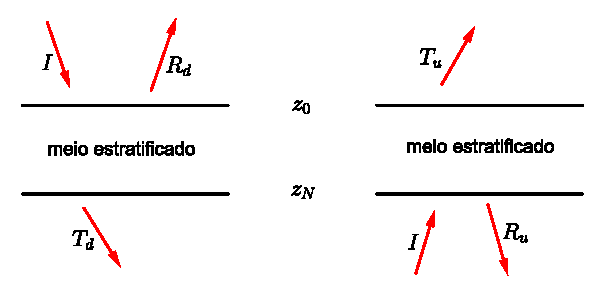
\includegraphics[scale=1.6]{ondas_ascen_descen}
%\caption{\textit{Dire\c{c}\~ao e sentido de propaga\c{c}\~ao de ondas ascendentes e descendentes em camadas homog\^eneas.}}
%\label{fig.ondas_ascen_descen}
%\end{figure}
%Vamos usar a const\^ancia da fun\c{c}\~ao dada na equa\c{c}\~ao \ref{eq.G(V,W)} para igualar seus valores calculados no topo e no fundo da pilha de camadas. Mas aqui, vamos tomar as ondas $V$ e $W$ com for\c{c}a $I$ em sentido descendente e ascendente, respectivamente.  
%\begin{equation*}
%\begin{bmatrix}
%R_d^\top&I
%\end{bmatrix}
%\begin{bmatrix}
%0&I\\
%-I&0
%\end{bmatrix}
%\begin{bmatrix}
%T_u\\
%0
%\end{bmatrix}
%=
%\begin{bmatrix}
%0&T_d^\top
%\end{bmatrix}
%\begin{bmatrix}
%0&I\\
%-I&0
%\end{bmatrix}
%\begin{bmatrix}
%I\\
%R_u
%\end{bmatrix}\,,
%\end{equation*}
%de onde conclu\'imos que
%\begin{equation}\label{eq.T}
%T_u=T_d^\top\,.
%\end{equation}
%Podemos ainda calcular o valor da fun\c{c}\~ao usando somente ondas descendentes $G(V,V)$. Igualando seus valores para o topo e a base da pilha de camadas, temos
%\begin{equation*}
%\begin{bmatrix}
%R_d^\top&I
%\end{bmatrix}
%\begin{bmatrix}
%0&I\\
%-I&0
%\end{bmatrix}
%\begin{bmatrix}
%R_d\\
%0
%\end{bmatrix}
%=
%\begin{bmatrix}
%0&R_d^\top
%\end{bmatrix}
%\begin{bmatrix}
%0&I\\
%-I&0
%\end{bmatrix}
%\begin{bmatrix}
%I\\
%R_d
%\end{bmatrix}\,,
%\end{equation*}
%de onde conclu\'imos que 
%\begin{equation}\label{eq.R_d}
%R_d=R_d^\top\,.
%\end{equation}
%Analogamente, para ondas ascendentes $G(W,W)$, temos \begin{equation}\label{eq.R_u}
%R_u=R_u^\top\,.
%\end{equation}
%Utilizando as equa\c{c}\~oes \ref{eq.T}, \ref{eq.R_d} e \ref{eq.R_u}, podemos definir uma matriz $R$ onde as componentes representam todas as ondas refletidas e transmitidas,
%\begin{equation*}
%R=
%\begin{bmatrix}
%R_d&T_u\\
%T_d&R_u
%\end{bmatrix}\,,
%\end{equation*}
%e verificar que 
%\begin{equation*}
%R=R^\top\,.
%\end{equation*}
%A matriz $R$ est\'a relacionada \`a matriz $S$ usada em \textit{Teoria de Dispers\~ao} de ondas,
%\begin{equation*}
%S=
%\begin{bmatrix}
%T_d&R_u\\
%R_d&T_u
%\end{bmatrix}\,,
%\end{equation*}
%e a matriz $S$ relaciona, de forma linear, ondas saindo de uma pilha de camadas com ondas entrando na pilha,
%\begin{equation*}
%\begin{bmatrix}
%\mathbf{D}(z_N)\\
%\mathbf{U}(z_0)
%\end{bmatrix}
%=
%S(z_0,z_N)\,
%\begin{bmatrix}
%\mathbf{D}(z_0)\\
%\mathbf{U}(z_N)
%\end{bmatrix}\,.
%\end{equation*} 
%
%\subsection{Rela\c{c}\~ao das Matrizes de Transmiss\~ao e Reflex\~ao com a matriz de Propaga\c{c}\~ao}
%
%As matrizes de reflex\~ao e transmiss\~ao podem ser escritas em termos das submatrizes da matriz de propaga\c{c}\~ao, da seguinte forma:
%\begin{align}\nonumber
%T_u(z_0,z_N)&=Q_{11}^{-1}(z_N,z_0)\,,\\\nonumber
%R_u(z_0,z_N)&=Q_{21}(z_N,z_0)\,Q_{11}^{-1}(z_N,z_0)\,,\\\label{eq.relacao_Q_R_T}
%R_d(z_0,z_N)&=-Q_{11}^{-1}(z_N,z_0)\,Q_{12}(z_N,z_0)\,,\\\nonumber
%T_d(z_0,z_N)&=Q_{22}(z_N,z_0)-Q_{21}(z_N,z_0)\,Q_{11}^{-1}(z_N,z_0)\,Q_{12}(z_N,z_0)\,,
%\end{align}
%e a matriz de propaga\c{c}\~ao \'e dada em fun\c{c}\~ao das matrizes de reflex\~ao e transmiss\~ao por
%\begin{equation*}
%Q(z_0,z_N)=
%\begin{bmatrix}
%T_u^{-1}&-T_u^{-1}R_d\\
%R_uT_u^{-1}&T_d-R_uT_u^{-1}R_d
%\end{bmatrix}\,.
%\end{equation*}
%
%
%Para o caso de camadas homog\^eneas, usando as equa\c{c}\~oes \ref{eq.Q(z,z_0)} e \ref{eq.relacao_Q_R_T}, podemos deduzir que, para matrizes de transmiss\~ao,
%\begin{equation*}
%T_d(z_0,z)=T_u(z_0,z)=\exp\left[\pm i\omega\,\Lambda(z-z_0)\right]\,,
%\end{equation*}
%e para matrizes de reflex\~ao
%\begin{equation*}
%R_d(z_0,z)=R_u(z_0,z)=0\,.
%\end{equation*}
%
%Vamos definir $E_{k+1}(-\pm i\omega)=\exp\left[-\pm i\omega\,\Lambda(z_{k+1}-z_k)\right]$. Assim, a matriz $S$ para uma camada homog\^enea e para interface para a pr\'oxima camada \'e dada pelo \textit{produto estrela},
%\begin{align*}
%S(z_{k+},z_{k+1+})&=S(z_{k+},z_{k+1-})*S(z_{k+1-},z_{k+1+})\\\\
%&=
%\begin{bmatrix}
%E_{k+1}(-\pm i\omega)&0\\
%0&E_{k+1}(-\pm i\omega)
%\end{bmatrix}
%*
%\begin{bmatrix}
%T_{d,k+1}&R_{u,k+1}\\
%R_{d,k+1}&T_{u,k+1}
%\end{bmatrix}\\\\
%&=
%\begin{bmatrix}
%T_{d,k+1}E_{k+1}(-\pm i\omega)&R_{u,k+1}\\
%E_{k+1}(-\pm i\omega)R_{d,k+1}E_{k+1}(-\pm i\omega)&E_{k+1}(-\pm i\omega)T_{u,k+1}
%\end{bmatrix}\,.
%\end{align*}
\chapter{An\'alise de Dispers\~ao e Atenua\c{c}\~ao de Ondas da Magneto-Elasticidade}

Neste cap\'itulo apresentaremos a an\'alise de dispers\~ao e atenua\c{c}\~ao de ondas mec\^anicas e ondas eletromagn\'eticas do efeito magneto-el\'astico. Primeiramente, seguiremos o desenvolvimento apresentado por \cite{Blanc_13} para realizar a an\'alise de dispers\~ao e atenua\c{c}\~ao para o caso particular de propaga\c{c}\~ao de ondas em uma \'unica dimens\~ao. Tal procedimento pode ser encontrado tamb\'em em \cite{oliveira_2018} e \cite{miranda_2016}, e \'e importante pois o estudo de casos mais simples de um problema facilita o entendimento da teoria e posterior abordagem de casos mais gerais e complexos. Em seguida, apresentaremos a an\'alise para o caso geral de propaga\c{c}\~ao de ondas no espa\c{c}o 3D, seguindo um outro desenvolvimento, aquele apresentado em \cite{sharma_08}.

\section{An\'alise de Dispers\~ao e Atenua\c{c}\~ao no Espa\c{c}o 1D}

Transformando do espa\c{c}o 3D para o espa\c{c}o 1D e linearizando as equa\c{c}\~oes da magneto-elasticidade do sistema apresentado no cap\'itulo \ref{sec.recon_model_dun_eri}, considerando somente a profundidade das camadas estratigr\'aficas como espa\c{c}o de propaga\c{c}\~ao de ondas, temos o seguinte sistema de EDP's do efeito magneto-el\'astico para o espa\c{c}o 1D
\begin{align}\label{eq.edp1}
\rho\frac{\partial^2u}{\partial\,t^2}&=\frac{\partial}{\partial\,z}\left[(\lambda+2\,G)\frac{\partial\,u}{\partial\,z}-\mu h^0h\right]+F\\\nonumber\\\label{eq.edp2}
\frac{\partial\,h}{\partial\,t}&=\frac{\partial}{\partial\,z}\left(V_H\frac{\partial\,h}{\partial\,z}-h^0\frac{\partial\,u}{\partial\,t}\right),
\end{align}
onde:
\begin{itemize}
\item $u$ \'e o deslocamento do meio;
\item $h$ \'e a varia\c{c}\~ao magn\'etica gerada;
\item $\lambda$ e $G$ s\~ao os par\^ametros de Lam\`e;
\item $t$ \'e o tempo;
\item $z$ \'e a profundidade;
\item $\rho$ \'e a densidade do meio;
\item $\mu$ \'e a permeabilidade magn\'etica do meio;
\item $h^0$ \'e o campo magn\'etico externo ao sistema (pode ser o geomagn\'etico);
\item $F$ \'e uma for\c{c}a externa fonte de onda s\'ismica;
\item $\sigma$ \'e a condutividade do meio, e
\item $V_H=(\sigma\,\mu)^{-1}$ \'e a viscosidade magn\'etica.
\end{itemize}

Segundo \cite{Blanc_13}, podemos utilizar solu\c{c}\~oes em termos de ondas planas para fazer an\'alise de dispers\~ao e atenua\c{c}\~ao das ondas que se propagam de acordo com o sistema de EDP's dado pelas equa\c{c}\~oes \ref{eq.edp1} e \ref{eq.edp2}.

Assim, sendo $\omega$ a frequ\^encia angular, $k$ o n\'umero de onda e $h_0$ e $u_0$ constantes n\~ao nulas, vamos substituir as solu\c{c}\~oes dadas por 
\begin{align}\label{eq.ondas_planas_1}
u&=u_0e^{i(\omega\,t-k\,z)}\\\label{eq.ondas_planas_2}
h&=h_0e^{i(\omega\,t-k\,z)},
\end{align}
na equa\c{c}\~ao \ref{eq.edp1} e obtermos
\begin{align}\nonumber
\rho\frac{\partial^2}{\partial\,t^2}u_0e^{i(\omega\,t-k\,z)}&=\frac{\partial}{\partial\,z}\left[(\lambda+2\,G)\frac{\partial}{\partial\,z}u_0e^{i(\omega\,t-k\,z)}-\mu h^0h_0e^{i(\omega\,t-k\,z)}\right]+F\,\Rightarrow\\\nonumber\\\nonumber
\rho\,u_0\frac{\partial^2}{\partial\,t^2}e^{i(\omega\,t-k\,z)}&=\frac{\partial}{\partial\,z}\left[(\lambda+2\,G)\,u_0\frac{\partial}{\partial\,z}\,e^{i(\omega\,t-k\,z)}-\mu h^0h_0e^{i(\omega\,t-k\,z)}\right]+F\,\Rightarrow\\\nonumber\\\nonumber
\rho\,u_0\frac{\partial}{\partial\,t}e^{i(\omega\,t-k\,z)}\,i\,\omega&=\frac{\partial}{\partial\,z}\left[(\lambda+2\,G)\,u_0e^{i(\omega\,t-k\,z)}(-i\,k)-\mu h^0h_0e^{i(\omega\,t-k\,z)}\right]+F\,\Rightarrow\\\nonumber\\\nonumber
i\,\omega\,\rho\,u_0e^{i(\omega\,t-k\,z)}\,i\,\omega&=-i\,k\,u_0(\lambda+2\,G)\,e^{i(\omega\,t-k\,z)}(-i\,k)-\mu h^0h_0e^{i(\omega\,t-k\,z)}(-i\,k)+F\,\Rightarrow\\\nonumber\\\nonumber
-\omega^2\rho\,u_0e^{i(\omega\,t-k\,z)}&=-k^2u_0(\lambda+2\,G)\,e^{i(\omega\,t-k\,z)}+i\,k\mu h^0h_0e^{i(\omega\,t-k\,z)}+F\,\Rightarrow\\\nonumber\\\label{eq.dedu_1}
-\omega^2\rho\,u_0&=-k^2u_0(\lambda+2\,G)+i\,k\mu h^0h_0+F\,e^{-i(\omega\,t-k\,z)}
\end{align}

Analogamente, substituindo as solu\c{c}\~oes \ref{eq.ondas_planas_1} e \ref{eq.ondas_planas_2} na equa\c{c}\~ao \ref{eq.edp2}, obtemos

\begin{align}\nonumber
\frac{\partial}{\partial\,t}\,h_0e^{i(\omega\,t-k\,z)}&=\frac{\partial}{\partial\,z}\left(V_H\frac{\partial}{\partial\,z}\,h_0e^{i(\omega\,t-k\,z)}-h^0\frac{\partial}{\partial\,t}\,u_0e^{i(\omega\,t-k\,z)}\right)\,\Rightarrow\\\nonumber\\\nonumber
h_0e^{i(\omega\,t-k\,z)}\,i\,\omega&=\frac{\partial}{\partial\,z}\left(V_Hh_0e^{i(\omega\,t-k\,z)}(-i\,k)-h^0u_0e^{i(\omega\,t-k\,z)}\,i\,\omega\right)\,\Rightarrow\\\nonumber\\\label{eq.dedu_2}
i\,\omega\,h_0e^{i(\omega\,t-k\,z)}&=-i\,k\,V_Hh_0e^{i(\omega\,t-k\,z)}(-i\,k)-i\,\omega
\,h^0u_0e^{i(\omega\,t-k\,z)}(-i\,k).
\end{align}
Considerando que $e^{\pm i(\omega\,t-k\,z)}\neq\,0$ em todo o dom\'inio e que para fins de an\'alise de dispers\~ao e atenua\c{c}\~ao n\~ao \'e necess\'aria a aplica\c{c}\~ao de for\c{c}a externa, as equa\c{c}\~oes \ref{eq.dedu_1} e \ref{eq.dedu_2} formam o seguinte sistema

\begin{empheq}[left=\empheqlbrace]{align*}
-\omega^2\rho\,u_0&=-k^2u_0(\lambda+2\,G)+i\,k\mu h^0h_0\\\\
i\,\omega\,h_0&=-k^2V_Hh_0-\omega\,k\,h^0u_0,
\end{empheq}\\

\begin{equation}
\begin{pmatrix}
k^2(\lambda+2\,G)-\omega^2\rho & -i\,k\mu h^0\\
\omega\,k\,h^0 & i\,\omega+k^2V_H
\end{pmatrix}
\begin{pmatrix}
u_0\\
h_0
\end{pmatrix}
=
\begin{pmatrix}
0\\
0
\end{pmatrix}.
\end{equation}\\

%\begin{empheq}[left=\empheqlbrace]{align*}
%h_0&=\frac{k^2(\lambda+2\,G)}{i\,k\mu h^0}\,u_0-\frac{\omega^2\rho}{i\,k\mu h^0}\,u_0\\\\
%h_0&=\frac{-\omega\,k\,h^0}{i\,\omega+k^2V_H}u_0.
%\end{empheq}\\

%Eliminando $h_0$, temos
%\begin{equation*}
%\left(\frac{k^2(\lambda+2\,G)-\omega^2\rho}{i\,k\mu h^0}+\frac{\omega\,k\,h^0}{i\,\omega+k^2V_H}\right)u_0=0.
%\end{equation*}\\

For\c{c}ando uma solu\c{c}\~ao n\~ao trivial, temos\\
\begin{equation*}
\frac{k^2(\lambda+2\,G)-\omega^2\rho}{i\,k\mu h^0}=-\frac{\omega\,k\,h^0}{i\,\omega+k^2V_H}\,\Rightarrow
\end{equation*}
\begin{align*}
i\,\omega\,k^2(\lambda+2\,G)-i\,\omega^3\rho+k^4V_H(\lambda+2\,G)-\omega^2k^2\rho\,V_H+i\,k^2\omega\,\mu(h^0)^2&=0\,\Rightarrow\\\\
V_H(\lambda+2\,G)\,k^4+\left[i\,\omega\,(\lambda+2\,G)+i\,\omega\,\mu(h^0)^2-\omega^2\rho\,V_H\right]\,k^2-i\,\omega^3\rho&=0.    
\end{align*}

A \'ultima igualdade, uma equa\c{c}\~ao biquadrada no n\'umero de onda, \'e a rela\c{c}\~ao de dispers\c{c}\~ao para ondas compressionais e eletro-magn\'eticas em meios isotr\'opicos, uma vez que o problema da magneto-elasticidade unidimensional n\~ao apresenta ondas cisalhantes.

Definindo 
\begin{align*}
D_4&=V_H(\lambda+2\,G)\\
D_2&=i\,\omega\,(\lambda+2\,G)+i\,\omega\,\mu(h^0)^2-\omega^2\rho\,V_H\\
D_0&=-i\,\omega^3\rho,
\end{align*}
temos que a rela\c{c}\~ao de dispers\~ao pode ser escrita como
\begin{equation*}
D_4k^4+D_2k^2+D_0=0,
\end{equation*}
onde os autovalores $k_j$ para $j=1,2,3,4$ s\~ao
\begin{equation*}
k=\pm\left(\frac{-D_2\pm\sqrt{D_2^2-4\,D_4D_0}}{2\,D_4}\right)^\frac{1}{2}.
\end{equation*}

Definindo $k_{P}$ como os autovalores para ondas compressionais e $k_{em}$ como autovalores para ondas eletro-magn\'eticas, temos
\begin{align*}
k_{P}&=\pm\left(\frac{-D_2+\sqrt{D_2^2-4\,D_4D_0}}{2\,D_4}\right)^\frac{1}{2}\\
k_{em}&=\pm\left(\frac{-D_2-\sqrt{D_2^2-4\,D_4D_0}}{2\,D_4}\right)^\frac{1}{2}.
\end{align*}
Contudo, simula\c{c}\~oes num\'ericas tem mostrado que podemos aproximar os autovalores por
\begin{align*}
k_{P}&=\left(\frac{-D_2+\sqrt{D_2^2-D_4D_0}}{D_4}\right)^\frac{1}{2}\\
k_{em}&=\left(\frac{-D_2-\sqrt{D_2^2-4\,D_4D_0}}{2\,D_4}\right)^\frac{1}{2}.
\end{align*}


Dessa forma, as velocidades de fases para ondas compressionais e eletro-magn\'eticas s\~ao, respectivamente,
\begin{equation*}
c_{P}=\frac{\omega}{\text{Re}(k_{P})}\quad\text{e}\quad c_{em}=\frac{\omega}{\text{Re}(k_{em})}.
\end{equation*}
E as respectivas atenua\c{c}\~oes s\~ao dadas por
\begin{equation*}
\alpha_{P}=-\text{Im}(k_{P})\quad\text{e}\quad \alpha_{em}=-\text{Im}(k_{em}).
\end{equation*}

As propriedades f\'isicas do meio de propaga\c{c}\~ao das ondas podem ser encontradas na tabela \ref{tab.dados_dispersao}, e seus valores s\~ao utilizados como par\^ametros nos c\'alculos da dispers\~ao e atenua\c{c}\~ao das ondas el\'asticas e eletromagn\'eticas. Algumas dessas propriedades foram extra\'idas de \cite{White_Zhou_2006} e outras de \cite{griffiths}.


\begin{table}
\begin{center}
\begin{tabular}{|c|c|c|c|}
\hline 
Propriedade & S\'imbolo & Valor & Unidade \\ 
\hline 
Massa espec\'ifica do meio & $\rho$ & 2400 & $Kg/m^3$ \\ 
\hline 
Par\^ametro de Lam\`e & $\lambda$ & $2.69\times 10^9$ & $Pa$ \\ 
\hline 
M\'odulo de cisalhamento & $G$ & $3.46\times 10^9$ & $Pa$ \\ 
\hline 
Viscosidade magn\'etica & $V_H$ & $7.9578\times 10^{-6}$ & $m^2/s$ \\ 
\hline 
Permeabilidade magn\'etica do meio & $\mu$ & $4\,\pi\times 10^{-7}$ & $T\,m/A$ \\ 
\hline 
Campo geomagn\'etico & $h^0$ & $4.625\times 10^{-5}$ & $T$ \\ 
\hline 
Condutividade & $\sigma$ & 0.1 & $S/m$ \\
\hline
\end{tabular}
\end{center}
\caption{\textit{Dados para realiza\c{c}\~ao da an\'alise de dispers\~ao e atenua\c{c}\~ao de ondas.}}
\label{tab.dados_dispersao}
\end{table}

Observe, ainda na tabela \ref{tab.dados_dispersao}, que estamos considerando a permeabilidade magn\'etica do meio igual \`a do v\'acuo, e as unidades de medida \textit{Tesla} e \textit{Siemens} s\~ao dadas, respectivamente, por $Vs/m^2$ e $A/V$, onde $A$ \'e o \textit{Ampere} e $V$ \'e o \textit{Volt}.

\begin{figure}
\centering
\subfloat{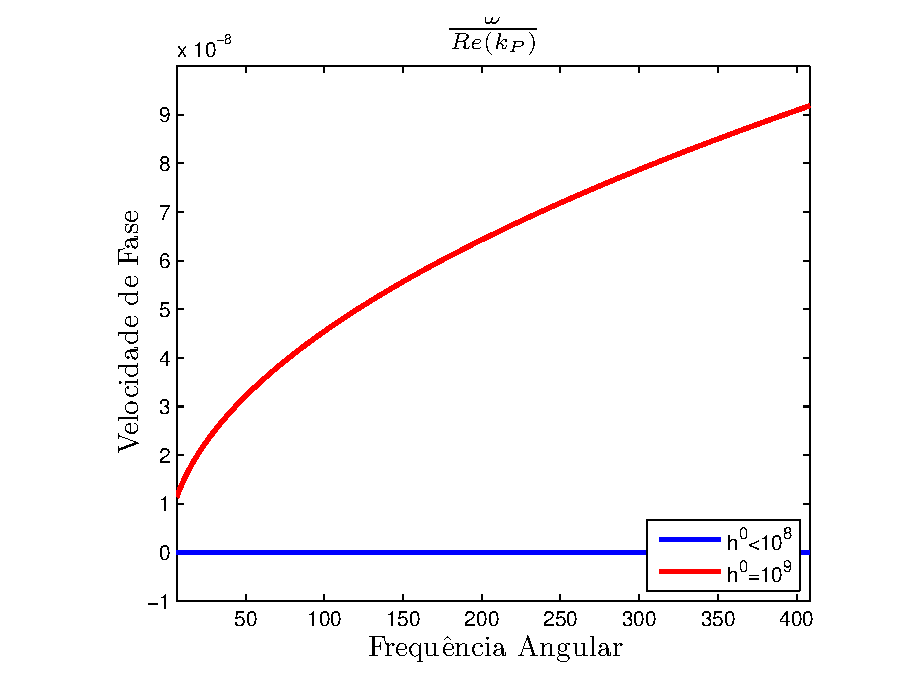
\includegraphics[scale=.57]{veloc_fase_P_1D}}
\subfloat{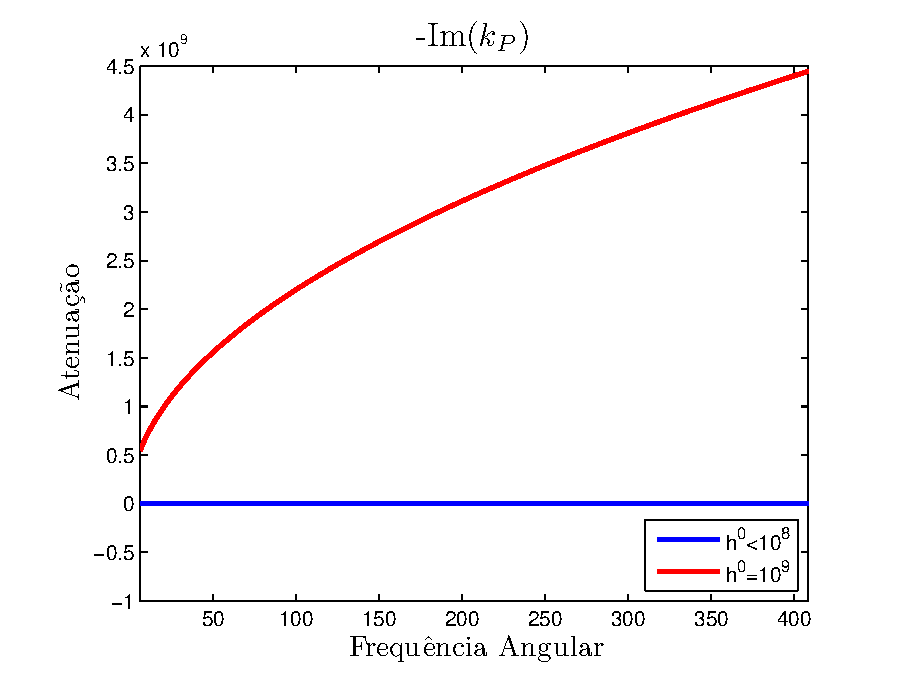
\includegraphics[scale=.57]{atenu_P_1D}}
\caption{\textit{Dispers\~ao e atenua\c{c}\~ao da onda compressional em fun\c{c}\~ao da frequ\^encia angular e de um campo magn\'etico externo.}}
\label{fig.disp_P}
\end{figure}


No nosso modelo estamos considerando o tipo de acoplamento onde a aplica\c{c}\~ao de um campo magn\'etico externo ao meio de propaga\c{c}\~ao influ\^encia a dispers\~ao e atenua\c{c}\~ao de ondas el\'asticas e eletromagn\'eticas. Sendo assim, na figura \ref{fig.disp_P} podemos observar o gr\'afico da velocidade de fase da onda el\'astica compressional em fun\c{c}\~ao da frequ\^encia angular e em fun\c{c}\~ao de um campo magn\'etico externo. Observamos pelo gr\'afico em azul que n\~ao h\'a dispers\~ao de ondas compressionais causada pela aplica\c{c}\~ao de um campo magn\'etico externo quando este atinge o valor de at\'e $10^8$ \textit{Tesla}. \'E natural que ocorra dispers\~ao de ondas compressionais causada por outros fatores. No entanto, nem mesmo com o aumento da frequ\^encia angular ocorre dispers\~ao da onda compressional causada pelo campo magn\'etico externo dentro do limite citado. Quando o campo magn\'etico externo atinge o valor $10^9$ \textit{Tesla}, podemos observar no gr\'afico em vermelho sua influ\^encia na dispers\~ao da onda compressional. Ou seja, o valor da dispers\~ao aumenta \`a medida que aumentamos o valor da frequ\^encia angular, mesmo que esse aumento na dispers\~ao n\~ao seja t\~ao significativo. Resumindo, na propaga\c{c}\~ao de ondas acopladas, o aumento extremo de um campo magn\'etico externo pode influenciar a dispers\~ao de uma onda mec\^anica compressional.


Analogamente ao que ocorre com a dispers\~ao de uma onda compressional, a atenua\c{c}\~ao dessa onda n\~ao \'e alterada pela aplica\c{c}\~ao de uma campo magn\'etico externo ao meio de propaga\c{c}\~ao, quando este campo varia entre 0 e $10^8$ \textit{Tesla}, como podemos ver no gr\'afico azul da figura \ref{fig.disp_P}. Quando o campo magn\'etico externo atinge o valor $10^9$ \textit{Tesla}, ocorre uma altera\c{c}\~ao muito significativa na atenua\c{c}\~ao da onda compressional, ao contr\'ario do que ocorre com a dispers\~ao. Ou seja, \`a medida que a frequ\^encia angular aumenta, podemos ver no gr\'afico vermelho o aumento significativo da atenua\c{c}\~ao.

\begin{figure}
\centering
\subfloat{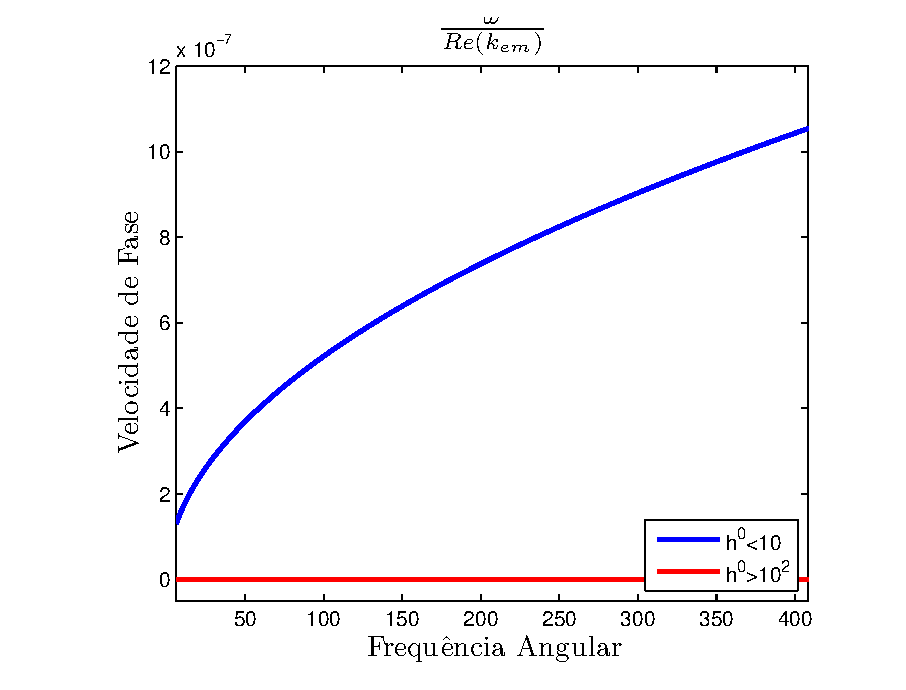
\includegraphics[scale=.57]{veloc_fase_em_1D}}
\subfloat{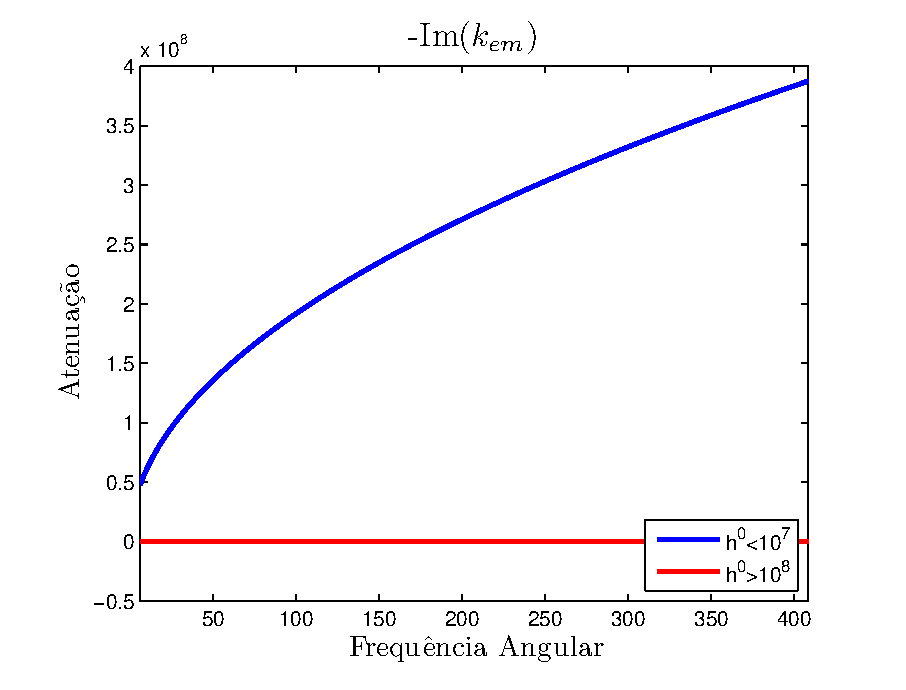
\includegraphics[scale=.57]{atenu_em_1D}}
\caption{\textit{Dispers\~ao e atenua\c{c}\~ao da onda eletromagn\'etica em fun\c{c}\~ao da frequ\^encia angular e de um campo magn\'etico externo.}}
\label{fig.disp_em}
\end{figure}

Na figura \ref{fig.disp_em}, podemos observar a varia\c{c}\~ao da velocidade de fase da onda eletromagn\'etica em fun\c{c}\~ao da varia\c{c}\~ao da frequ\^encia angular e em fun\c{c}\~ao do campo magn\'etico externo. Ao contr\'ario do que ocorre com a velocidade de fase da onda el\'astica, a velocidade de fase da onda eletromagn\'etica sofre altera\c{c}\~oes para valores pequenos do campo magn\'etico externo. Quando temos valores do campo magn\'etico externo at\'e 10 \textit{Tesla}, a velocidade de fase aumenta sutilmente \`a medida que a frequ\^encia angular varia de 0 a 400 \textit{Hz}. Quando o campo magn\'etico externo atinge valores maiores que $10^2$, n\~ao h\'a mais varia\c{c}\~ao da dispers\~ao da onda eletromagn\'etica.


Podemos observar a varia\c{c}\~ao da atenua\c{c}\~ao da onda eletromagn\'etica em fun\c{c}\~ao da frequ\^encia angular e em fun\c{c}\~ao do campo magn\'etico externo na figura \ref{fig.disp_em}. Para valores do campo magn\'etico externo entre 0 e $10^7$ \textit{Tesla}, existe um crescimento muito significativo na atenua\c{c}\~ao da onda eletromagn\'etica \`a medida que ocorre o aumento da frequ\^encia angular. Para valores do campo magn\'etico externo maiores que $10^8$ \textit{Tesla}, n\~ao h\'a mais varia\c{c}\~ao da atenua\c{c}\~ao da onda eletromagn\'etica, seu valor permanece constante e igual a zero. Observe que, quando comparamos as atenua\c{c}\~oes das ondas el\'astica e eletromagn\'etica, ocorre uma altern\^ancia no comportamento da mesma em fun\c{c}\~ao do campo magn\'etico externo. Enquanto que para a onda eletromagn\'etica ocorre altera\c{c}\~ao da atenua\c{c}\~ao ate $10^7$ \textit{Tesla}, a atenua\c{c}\~ao da onda el\'astica s\'o deixa de ser constante e igual a zero para valores grandes do campo magn\'etico externo, a partir de $10^9$ \textit{Tesla}. 


\section{An\'alise de Dispers\~ao e Atenua\c{c}\~ao no Espa\c{c}o 3D}

As equa\c{c}\~oes utilizadas para a an\'alise de dispers\~ao e atenua\c{c}\~ao s\~ao deduzidas a partir do modelo para o efeito magneto-el\'astico encontrado em \cite{eringen_1963}, conforme apresentado no cap\'itulo \ref{sec.model_dun_erin}. Essas equa\c{c}\~oes escritas no dom\'inio da frequ\^encia angular e simplificadas pelo regime quasi-estacion\'ario, similar ao que foi feito no cap\'itulo \ref{sec.recon_model_dun_eri}, s\~ao dadas por 


\begin{align}\label{eq.faraday}
\nabla\times\mathbf{\widehat{E}}&=i\,\omega\mu_0\mathbf{\widehat{H}}\\\nonumber\\\label{eq.ampere}
\nabla\times\mathbf{\widehat{H}}&=\mathbf{\widehat{J}}-i\,\epsilon\,\omega\,\mathbf{\widehat{E}}\\\nonumber\\\label{eq.div_B}
\nabla\cdot\mathbf{\widehat{H}}&=0\\\nonumber\\\label{eq.equi_couchy}
-i\,\omega\rho\,\mathbf{\widehat{v}}&=\nabla\cdot\widehat{\tau}+\rho_e\mathbf{\widehat{E}}+(\mathbf{\widehat{J}}\times\,\mu_0\mathbf{\widehat{H}})\\\nonumber\\\label{eq.dens_fluxo_ele}
\mathbf{\widehat{J}}&=\sigma\,(\mathbf{\widehat{E}}+\mathbf{\widehat{v}}\times\,\mu_0\mathbf{\widehat{H}})\\\nonumber\\\label{eq.Lame}
\widehat{\tau}&=\lambda\,(\nabla\cdot\mathbf{\widehat{u}})\,I + G\,(\nabla\,\mathbf{\widehat{u}}+\nabla\mathbf{\widehat{u}}^\top).
\end{align}

Substituindo a densidade de fluxo el\'etrico \ref{eq.dens_fluxo_ele} na equa\c{c}\~ao \ref{eq.ampere} e introduzindo o campo magn\'etico externo desprezando a parcela $\mathbf{\widehat{v}}\times\,\sigma\,\mu_0\mathbf{\widehat{H}}$, temos
\begin{equation*}
\nabla\times\mathbf{\widehat{H}}=(\sigma-i\,\epsilon\omega)\,\mathbf{\widehat{E}}+\mathbf{\widehat{v}}\times\,\sigma\,\mu_0\mathbf{\widehat{H}^0}.
\end{equation*}

Aplicando o rotacional na equa\c{c}\~ao acima e introduzindo a equa\c{c}\~ao \ref{eq.faraday}, temos
\begin{equation*}
\nabla\times(\nabla\times\mathbf{\widehat{H}})=(\sigma-i\,\epsilon\,\omega)\,i\,\omega\mu_0\mathbf{\widehat{H}}+\nabla\times(\mathbf{\widehat{v}}\times\,\sigma\,\mu_0\mathbf{\widehat{H}^0}).
\end{equation*}

Utilizando as rela\c{c}\~oes da \'algebra vetorial encontradas em JACKSON, a equa\c{c}\~ao acima se torna

\begin{align*}
\nabla(\nabla\cdot\mathbf{\widehat{H}})-\nabla^2\mathbf{\widehat{H}}&=(\sigma-i\,\epsilon\,\omega)\,i\,\omega\mu_0\mathbf{\widehat{H}}\\
&+\sigma\,\mu_0\left[(\nabla\cdot\mathbf{\widehat{H}^0})\,\mathbf{\widehat{v}}-(\nabla\cdot\mathbf{\widehat{v}})\,\mathbf{\widehat{H}^0}+(\mathbf{\widehat{H}^0}\cdot\nabla)\,\mathbf{\widehat{v}}-(\mathbf{\widehat{v}}\cdot\nabla)\,\mathbf{\widehat{H}^0}\right].
\end{align*}

Substituindo a equa\c{c}\~ao \ref{eq.div_B}, temos
\begin{equation*}
-\nabla^2\mathbf{\widehat{H}}=(\sigma-i\,\epsilon\,\omega)\,i\,\omega\mu_0\mathbf{\widehat{H}}+\sigma\,\mu_0\left[-(\nabla\cdot\mathbf{\widehat{v}})\,\mathbf{\widehat{H}^0}+(\mathbf{\widehat{H}^0}\cdot\nabla)\,\mathbf{\widehat{v}}\right].
\end{equation*}

Ou, considerando $\mathbf{\widehat{v}}=-i\,\omega\,\mathbf{\widehat{u}}$, podemos utilizar
\begin{equation}\label{eq.disp_1}
-\nabla^2\mathbf{\widehat{H}}=(\sigma-i\,\epsilon\,\omega)\,i\,\omega\mu_0\mathbf{\widehat{H}}+\nabla\times(-i\,\omega\,\mathbf{\widehat{u}}\times\,\sigma\,\mu_0\mathbf{\widehat{H}^0}).
\end{equation}

Desprezando a varia\c{c}\~ao do campo el\'etrico na equa\c{c}\~ao \ref{eq.ampere} e desprezando a densidade de carga el\'etrica na equa\c{c}\~ao \ref{eq.equi_couchy} ainda como consequ\^encia do regime quasi-estacion\'ario das equa\c{c}\~oes de Maxwell, podemos utilizar essas duas equa\c{c}\~oes para obter
\begin{equation*}
-i\,\omega\rho\,\mathbf{\widehat{v}}=\nabla\cdot\widehat{\tau}+(\nabla\times\mathbf{\widehat{H}})\times\,\mu_0\mathbf{\widehat{H}}.
\end{equation*}

Introduzindo o campo magn\'etico externo e desprezando a parcela $\mu_0\mathbf{\widehat{H}}$, temos a lineariza\c{c}\~ao
\begin{equation*}
-i\,\omega\rho\,\mathbf{\widehat{v}}=\nabla\cdot\widehat{\tau}+(\nabla\times\mathbf{\widehat{H}})\times\,\mu_0\mathbf{\widehat{H}^0}.
\end{equation*}

Aplicando o divergente na equa\c{c}\~ao \ref{eq.Lame} e substituindo na equa\c{c}\~ao acima juntamente com $\mathbf{\widehat{v}}=-i\,\omega\,\mathbf{\widehat{u}}$, temos
\begin{equation}\label{eq.disp_2}
-\omega^2\rho\,\mathbf{\widehat{u}}=\lambda\,\nabla\cdot[(\nabla\cdot\mathbf{\widehat{u}})\,I] + G\,\nabla\cdot(\nabla\,\mathbf{\widehat{u}}+\nabla\mathbf{\widehat{u}}^\top)+(\nabla\times\mathbf{\widehat{H}})\times\,\mu_0\mathbf{\widehat{H}^0}.
\end{equation}

Agora, podemos utilizar as equa\c{c}\~oes \ref{eq.disp_1} e \ref{eq.disp_2} para formar um sistema em termos dos campos el\'astico e magn\'etico, onde a an\'alise de dispers\~ao e atenua\c{c}\~ao pode ser realizada para ondas mec\^anicas e ondas eletromagn\'eticas separadamente,
\begin{empheq}[left=\empheqlbrace]{align*}
-\nabla^2\mathbf{\widehat{H}}&=(\sigma-i\,\epsilon\,\omega)\,i\,\omega\mu_0\mathbf{\widehat{H}}+\nabla\times(-i\,\omega\,\mathbf{\widehat{u}}\times\,\sigma\,\mu_0\mathbf{\widehat{H}^0})\\\\
-\omega^2\rho\,\mathbf{\widehat{u}}&=\lambda\,\nabla\cdot[(\nabla\cdot\mathbf{\widehat{u}})\,I] + G\,\nabla\cdot(\nabla\,\mathbf{\widehat{u}}+\nabla\mathbf{\widehat{u}}^\top)+(\nabla\times\mathbf{\widehat{H}})\times\,\mu_0\mathbf{\widehat{H}^0}.
\end{empheq}

Para efetuar a analise de dispersao e atenuacao usando o sistema acima, vamos utilizar o procedimento encontrado em \cite{sharma_08}. Sendo assim, ...








\chapter{Solu\c{c}\~oes N\'umericas e Anal\'iticas de Ondas do Efeito Magneto-El\'astico}

Neste cap\'itulo vamos abordar a propaga\c{c}\~ao de ondas do efeito magneto-el\'astico tanto para um meio homog\^eneo como para meios estratificados e homog\^eneos por camada, considerando a aplica\c{c}\~ao de uma fonte mec\^anica ou aplica\c{c}\~ao de uma fonte mec\^anica junto com uma fonte eletromagn\'etica, sendo quaisquer dos casos meios el\'asticos e condutivos que utilizam o regime \textit{quasi}-estacion\'ario das equa\c{c}\~oes de \textit{Maxwell}. Os modelos podem ainda ser escritos considerando a propaga\c{c}\~ao no espa\c{c}o 1D ou 3D, com campos mec\^anicos e eletromagn\'eticos totalmente ou parcialmente acoplados. Estamos aplicando hip\'oteses simplificadoras conforme cada situa\c{c}\~ao e, para o caso mais simples, conseguimos apresentar solu\c{c}\~oes anal\'iticas, e para os casos mais avan\c{c}ados vamos apresentar solu\c{c}\~oes num\'ericas baseadas no algoritmo matricial encontrado em \cite{Ursin-1983}. Como n\~ao \'e poss\'ivel ajustar as equa\c{c}\~oes do efeito magneto-el\'astico ao formato preconizado por \cite{Ursin-1983}, utilizamos o algoritmo com algumas pequenas adapta\c{c}\~oes. Em todas as figuras desse c\'apitulo vemos gr\'aficos em azul e gr\'aficos em vermelho, onde em azul temos informa\c{c}\~oes sobre tempo de chegada, amplitude e dispers\~ao, e em vermelho temos informa\c{c}\~oes sobre tempo de chegada e atenua\c{c}\~ao. Todas as simula\c{c}\~oes s\~ao executadas usando os dados da tabela (\ref{tab.dados_propagacao}) salvo poucas exce\c{c}\~oes descritas em cada caso, e as valida\c{c}\~oes do tempo de ocorr\^encia de cada evento \'e feita utilizando a velocidade de grupo para cada tipo de onda.

\begin{table}
\begin{center}
\begin{tabular}{|c|c|c|c|}
\hline 
Propriedade & Camada 1 & Camada 2 & Camada 3 \\ 
\hline 
Massa espec\'ifica do meio ($Kg/m^3$) & 2200 & 2400 & 2200 \\ 
\hline 
M\'odulo de compressibilidade ($Pa$) & $4,69\times 10^9$ & $2,69\times 10^9$ & $6,05\times 10^9$ \\ 
\hline 
M\'odulo de cisalhamento ($Pa$) & $3,46\times 10^9$ & $7,78\times 10^9$ & $1,46\times 10^9$ \\ 
\hline 
Viscosidade magn\'etica ($m^2/s$) & $3,97\times 10^{6}$ & $7,95\times 10^{5}$ & $2,65\times 10^{6}$ \\ 
\hline 
Permeabilidade magn\'etica do meio ($T\,m/A$) & $4\,\pi\times 10^{-7}$ & $4\,\pi\times 10^{-6}$ & $4\,\pi\times 10^{-7}$ \\ 
\hline 
Campo magn\'etico externo ($T$) & $10^{8}$ & $10^{8}$ & $10^{8}$ \\ 
\hline 
Condutividade ($S/m$) & 0,2 & 0,1 & 0,3 \\
\hline
\end{tabular}
\end{center}
\caption{\textit{Dados para simula\c{c}\~ao da propaga\c{c}\~ao de ondas.}}
\label{tab.dados_propagacao}
\end{table}

\section{Ondas em Meio Homog\^eneo se Propagando em uma Dimens\~ao}\label{sec.prop_homo_1D}
\subsection{Acoplamento Total}
Da mesma forma que fizemos com a an\'alise de dispers\~ao e atenua\c{c}\~ao, vamos come\c{c}ar a an\'alise de propaga\c{c}\~ao de ondas totalmente acopladas com um problema mais particular, para observarmos algum poss\'ivel comportamento que nos auxilie na resolu\c{c}\~ao de um problema mais geral. Assim, vamos substituir a equa\c{c}\~ao (\ref{eq.edo_2}) na derivada em rela\c{c}\~ao ao espa\c{c}o da equa\c{c}\~ao (\ref{eq.edo_3}) e isolar o campo magn\'etico para obter a equa\c{c}\~ao (\ref{eq.cam_mag_1D_homo}). Analogamente, vamos derivar a equa\c{c}\~ao (\ref{eq.edo_7}), substitu\'i-la na equa\c{c}\~ao (\ref{eq.edo_10}) e isolar o campo mec\^anico para obtermos a equa\c{c}\~ao (\ref{eq.cam_mech_1D_homo}).
\begin{align}\label{eq.cam_mech_1D_homo}
-\omega^2\rho\,u&=\frac{\partial}{\partial\,z}\left[(\lambda+2\,G)\frac{\partial\,u}{\partial\,z}-\mu h^0h\right]+F(z,\omega)\\\nonumber\\\label{eq.cam_mag_1D_homo}
-i\,\omega\,h&=\frac{\partial}{\partial\,z}\left(V_H\frac{\partial\,h}{\partial\,z}-h^0\frac{\partial\,u}{\partial\,t}\right).
\end{align}
Observe que estas equa\c{c}\~oes se encontram no dom\'inio da frequ\^encia e descrevem o acoplamento total entre as ondas mec\^anicas e eletromagn\'eticas. Aplicamos a transformada de Fourier e trabalhamos com os campos mec\^anico e magn\'etico na depend\^encia do n\'umero de onda,
\begin{align}
-\omega^2\rho\,u&=-k^2(\lambda+2\,G)\,u-i\,k\,\mu_0h^0h+F(k,\omega)\\\nonumber\\\
-i\,\omega\,h&=-k^2V_Hh-k\,\omega\,h^0u.
\end{align}
Definindo a fun\c{c}\~ao
\begin{equation}
g_1(k,\omega)=\frac{\omega\,k\,h^0}{i\,\omega-V_Hk^2},
\end{equation} 
temos que as solu\c{c}\~oes do sistema acima s\~ao dadas por
\begin{align*}
u(k,\omega)&=\frac{F(k,\omega)}{(\lambda+2\,G)\,k^2-\omega^2\rho+i\,k\,\mu_0h^0g_1(k,\omega)}\\
h(k,\omega)&=g_1(k,\omega)\,u(k,\omega).
\end{align*}

\subsection{Acoplamento Parcial}
Como \cite{Knopoff_1955} preconiza, a altera\c{c}\~ao que os campos geomagn\'eticos aplicam em campos mec\^anicos \'e desprez\'ivel, o que sugere que podemos desconsiderar a influ\^encia do campo magn\'etico externo em nosso modelo magneto-el\'astico para observarmos o resultado obtido. Portanto, vamos trabalhar com o acoplamento parcial que consiste em desprezar a parcela que cont\'em o campo magn\'etico na equa\c{c}\~ao (\ref{eq.cam_mech_1D_homo}). Para o acoplamento parcial, as solu\c{c}\~oes s\~ao dadas por
\begin{align*}
u_p(k,\omega)&=\frac{F(k,\omega)}{(\lambda+2\,G)\,k^2-\omega^2\rho}\\
h_p(k,\omega)&=g_1(k,\omega)\,u_p(k,\omega).
\end{align*}
Consideramos uma geometria estratigr\'afica composta por uma \'unica camada homog\^enea e com dimens\~oes infinitas, cujas caracter\'isticas est\~ao na coluna camada 1 da tabela (\ref{tab.dados_propagacao}). Na figura (\ref{fig.mech_homo_low_dep}) observamos tra\c{c}os s\'ismicos em fun\c{c}\~ao da dist\^ancia que os receptores se encontram da fonte, e quanto maior essa dist\^ancia menor \'e a amplitude dos tra\c{c}os. Temos um tra\c{c}o confeccionado usando o modelo de acoplamento total e o outro usando o modelo de acoplamento parcial, e vemos que n\~ao h\'a diferen\c{c}a entre os tra\c{c}os. Ou seja, para este modelo simples do efeito magneto-el\'astico (e para os pr\'oximos tamb\'em), a influ\^encia que campos eletromagn\'eticos exercem em campos mec\^anicos \'e desprez\'ivel. Podemos observar na figura (\ref{fig.mag_homo_low_dep}) exatamente a mesma abordagem anterior aplicada agora ao campo magn\'etico e, n\~ao importa se o acoplamento \'e total ou parcial, o comportamento permanece o mesmo. Comparando os gr\'aficos do campo magn\'etico com os do campo mec\^anico vemos que o campo magn\'etico sofre mais influ\^encia dos efeitos de dispers\~ao. Nas figuras (\ref{fig.mech_homo_high_dep}) e (\ref{fig.mag_homo_high_dep}), vemos que as caracter\'isticas de propaga\c{c}\~ao citadas acima continuam v\'alidas mesmo em caso de grandes dist\^ancias fonte/receptor.

\begin{landscape}
\begin{figure}
\centering
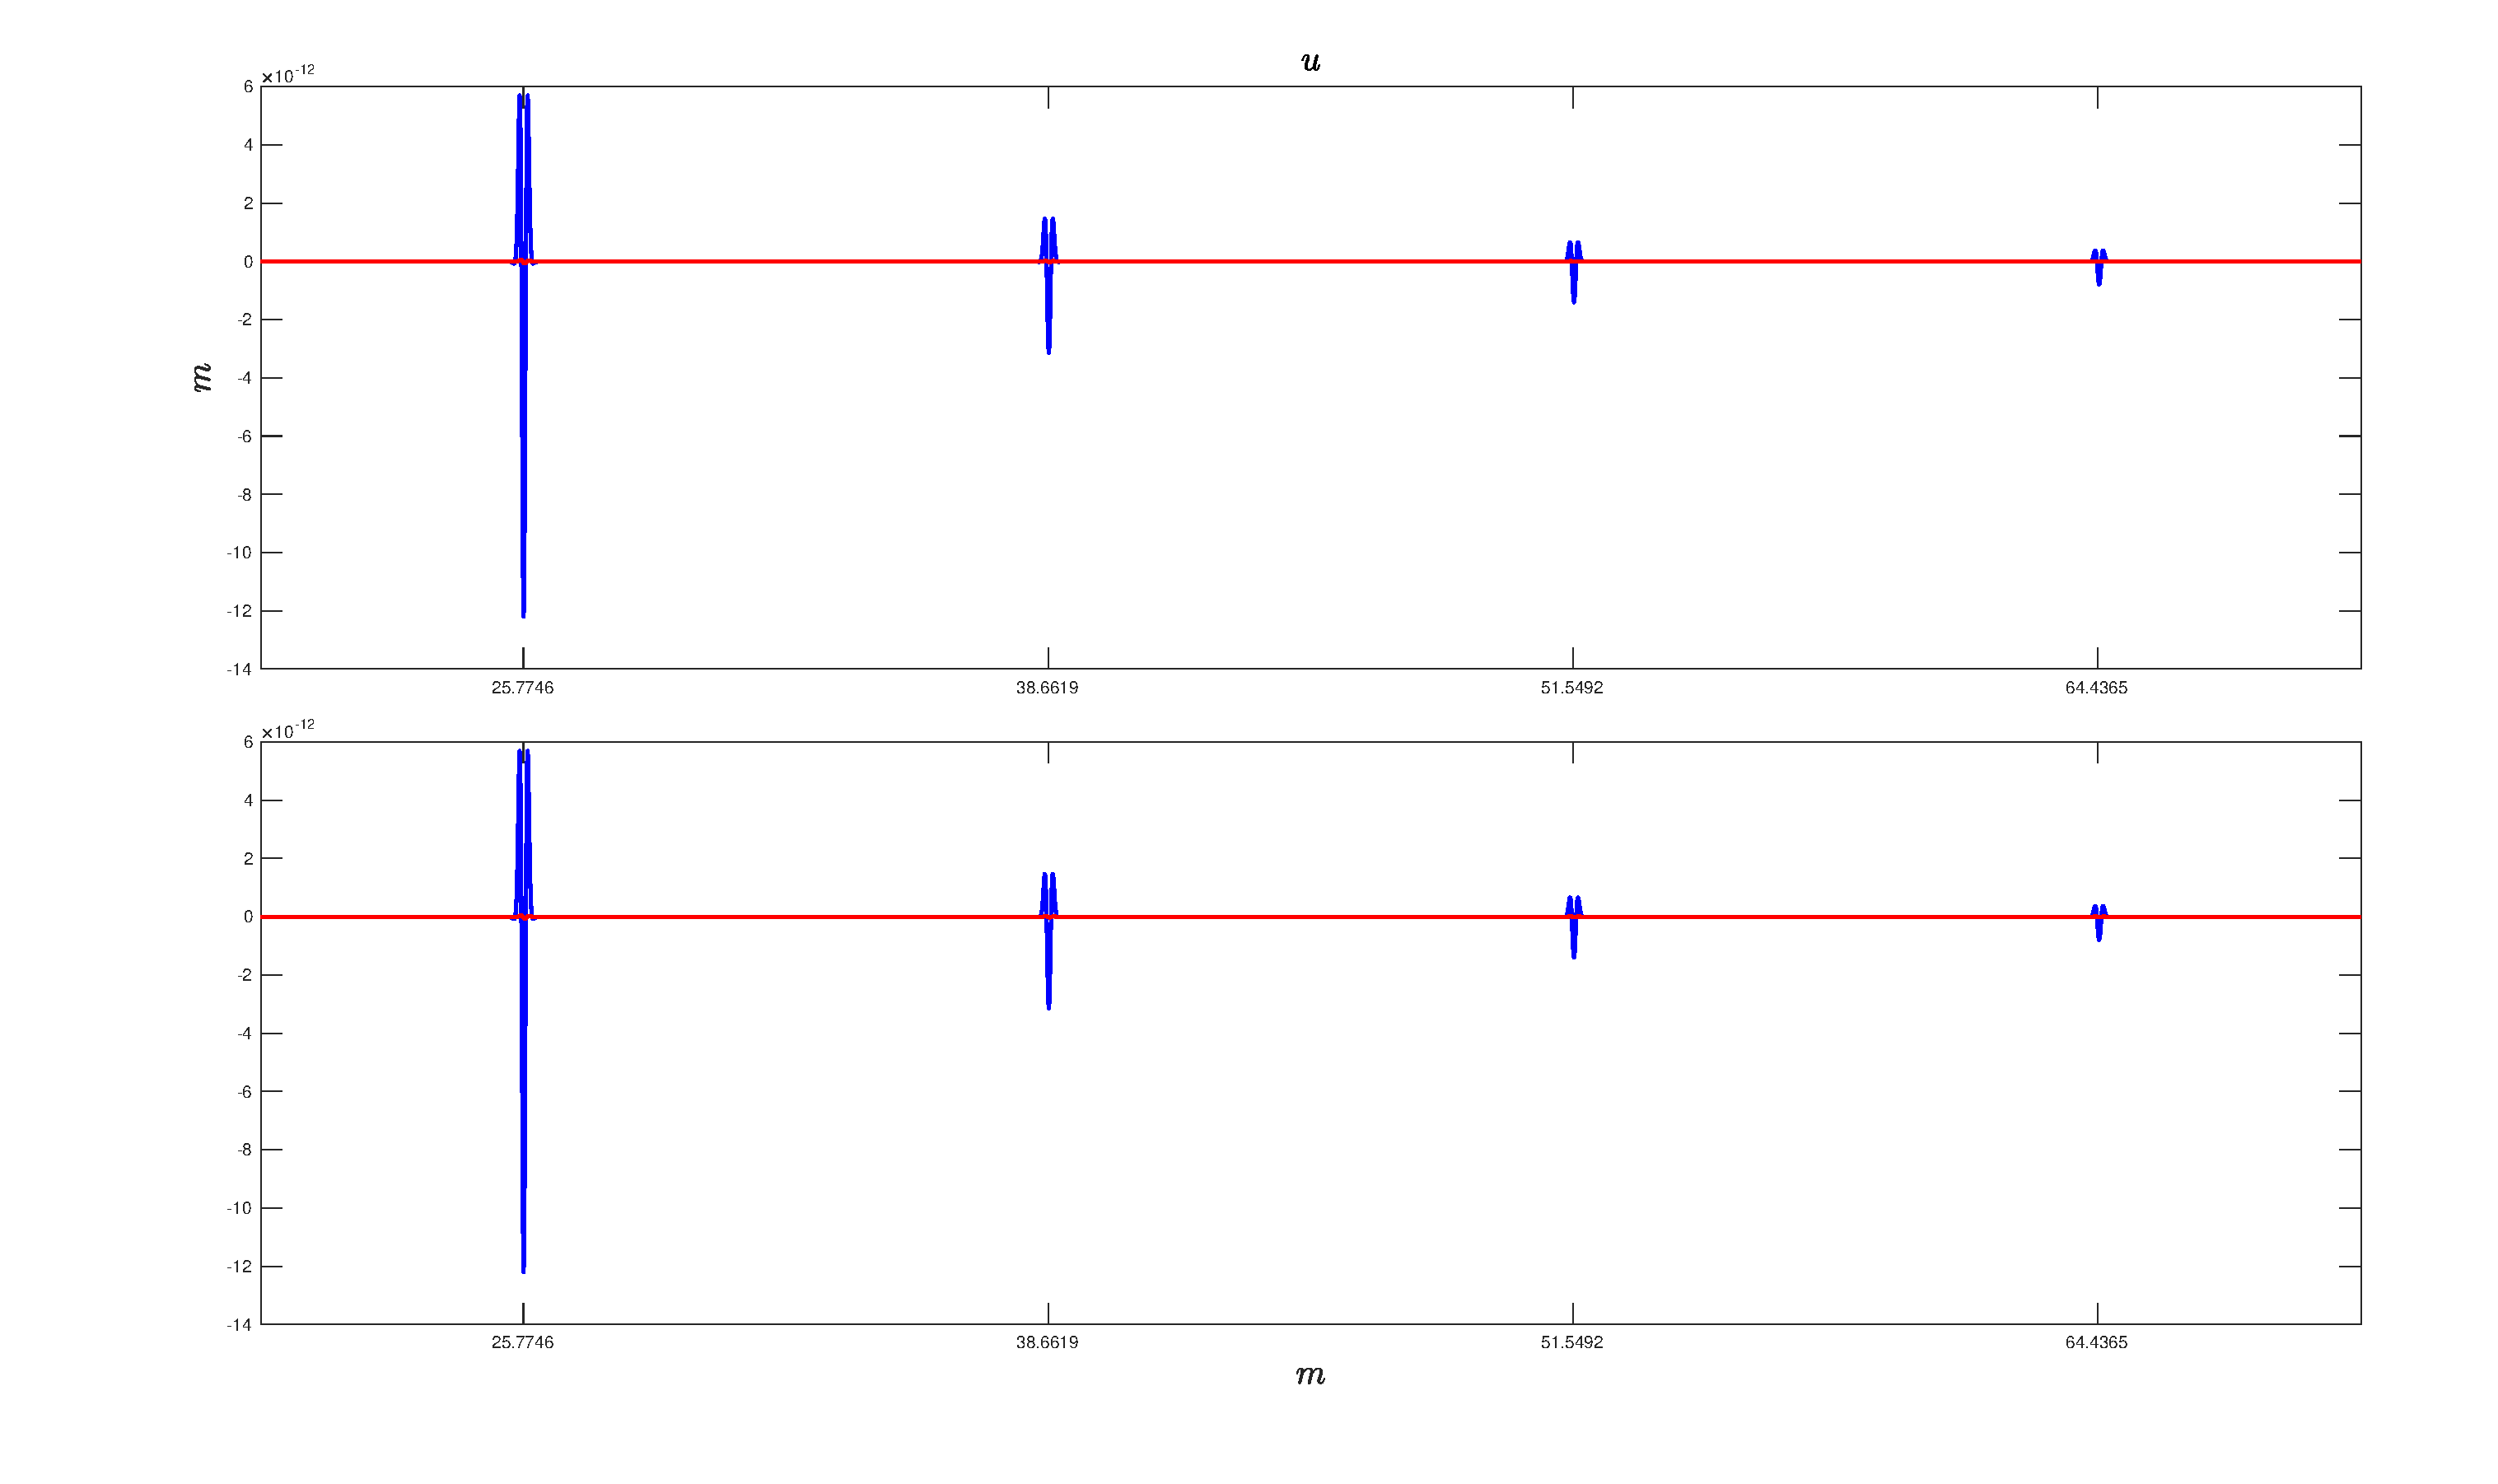
\includegraphics[scale=.5]{u_homo_F}
\caption{\textit{Tra\c{c}o s\'ismico de onda mec\^anica para sistema totalmente acoplado em cima e parcialmente acoplado embaixo, para pequenas dist\^ancias fonte/receptor.}}
\label{fig.mech_homo_low_dep}
\end{figure}
\end{landscape}

\begin{landscape}
\begin{figure}
\centering
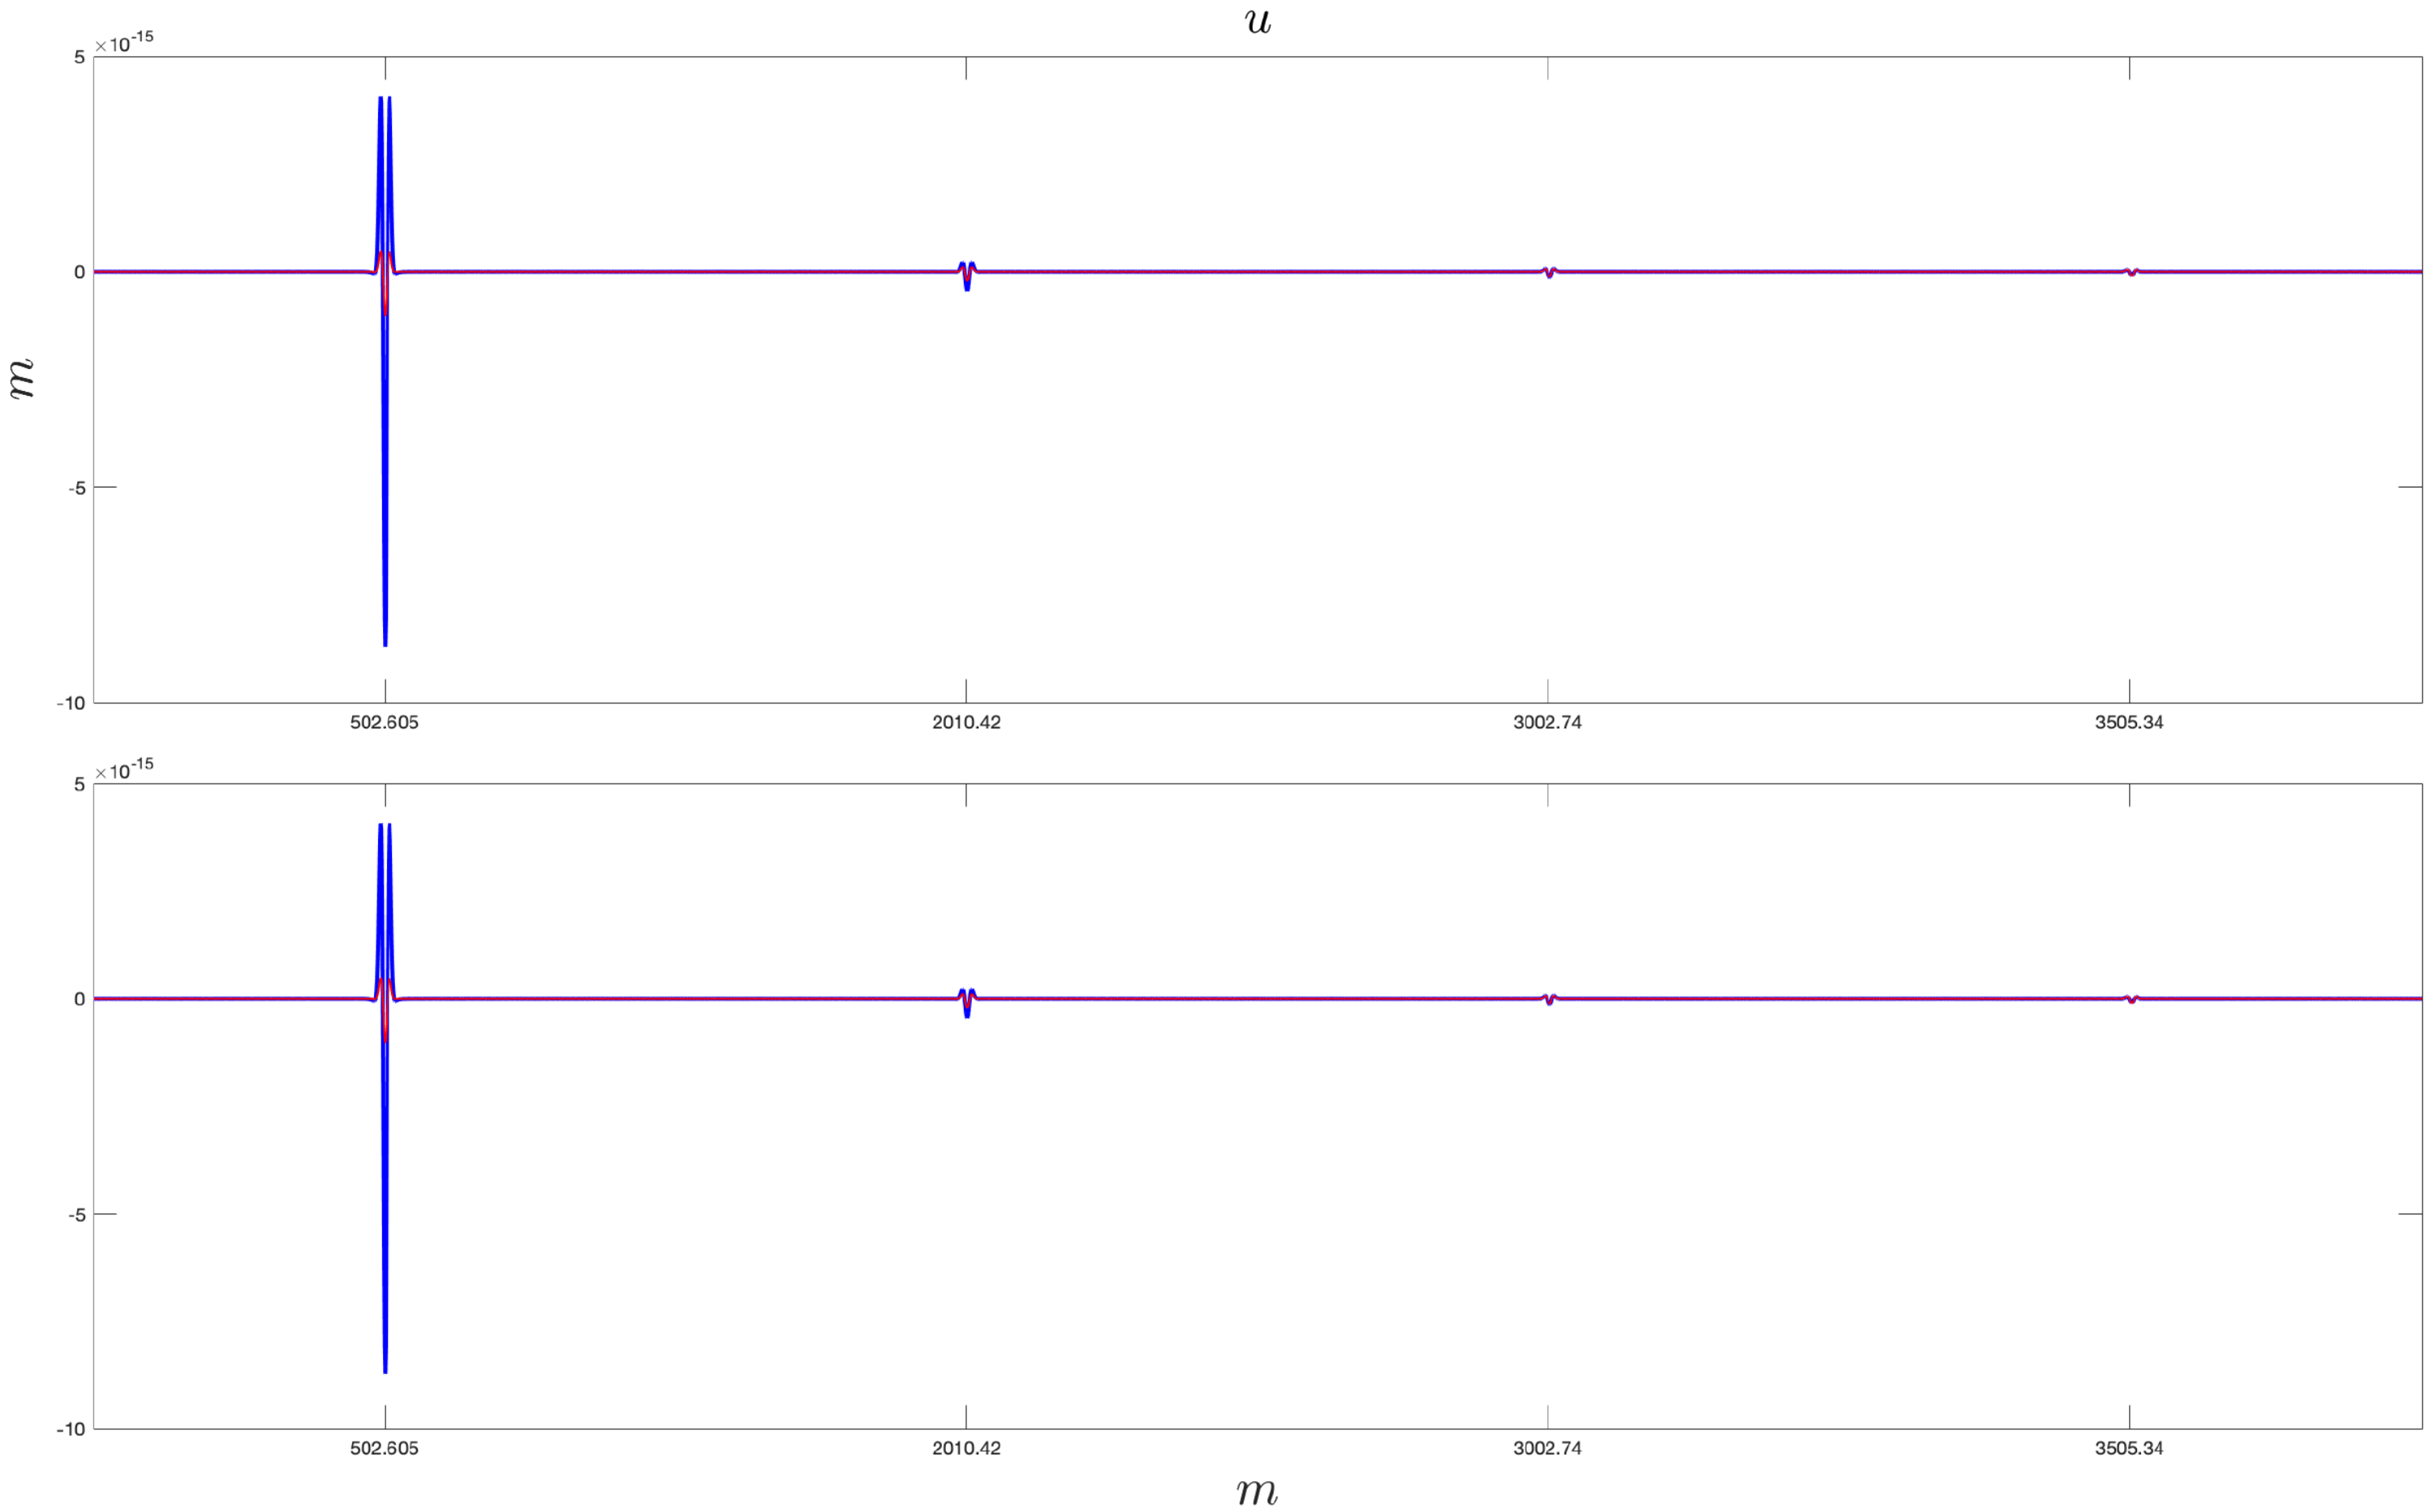
\includegraphics[scale=1.05]{u_homo_large_depth}
\caption{\textit{Tra\c{c}o s\'ismico de onda mec\^anica para sistema totalmente acoplado em cima e parcialmente acoplado embaixo, para grandes dist\^ancias fonte/receptor.}}
\end{figure}
\label{fig.mag_homo_low_dep}
\end{landscape}

\begin{landscape}
\begin{figure}
\centering
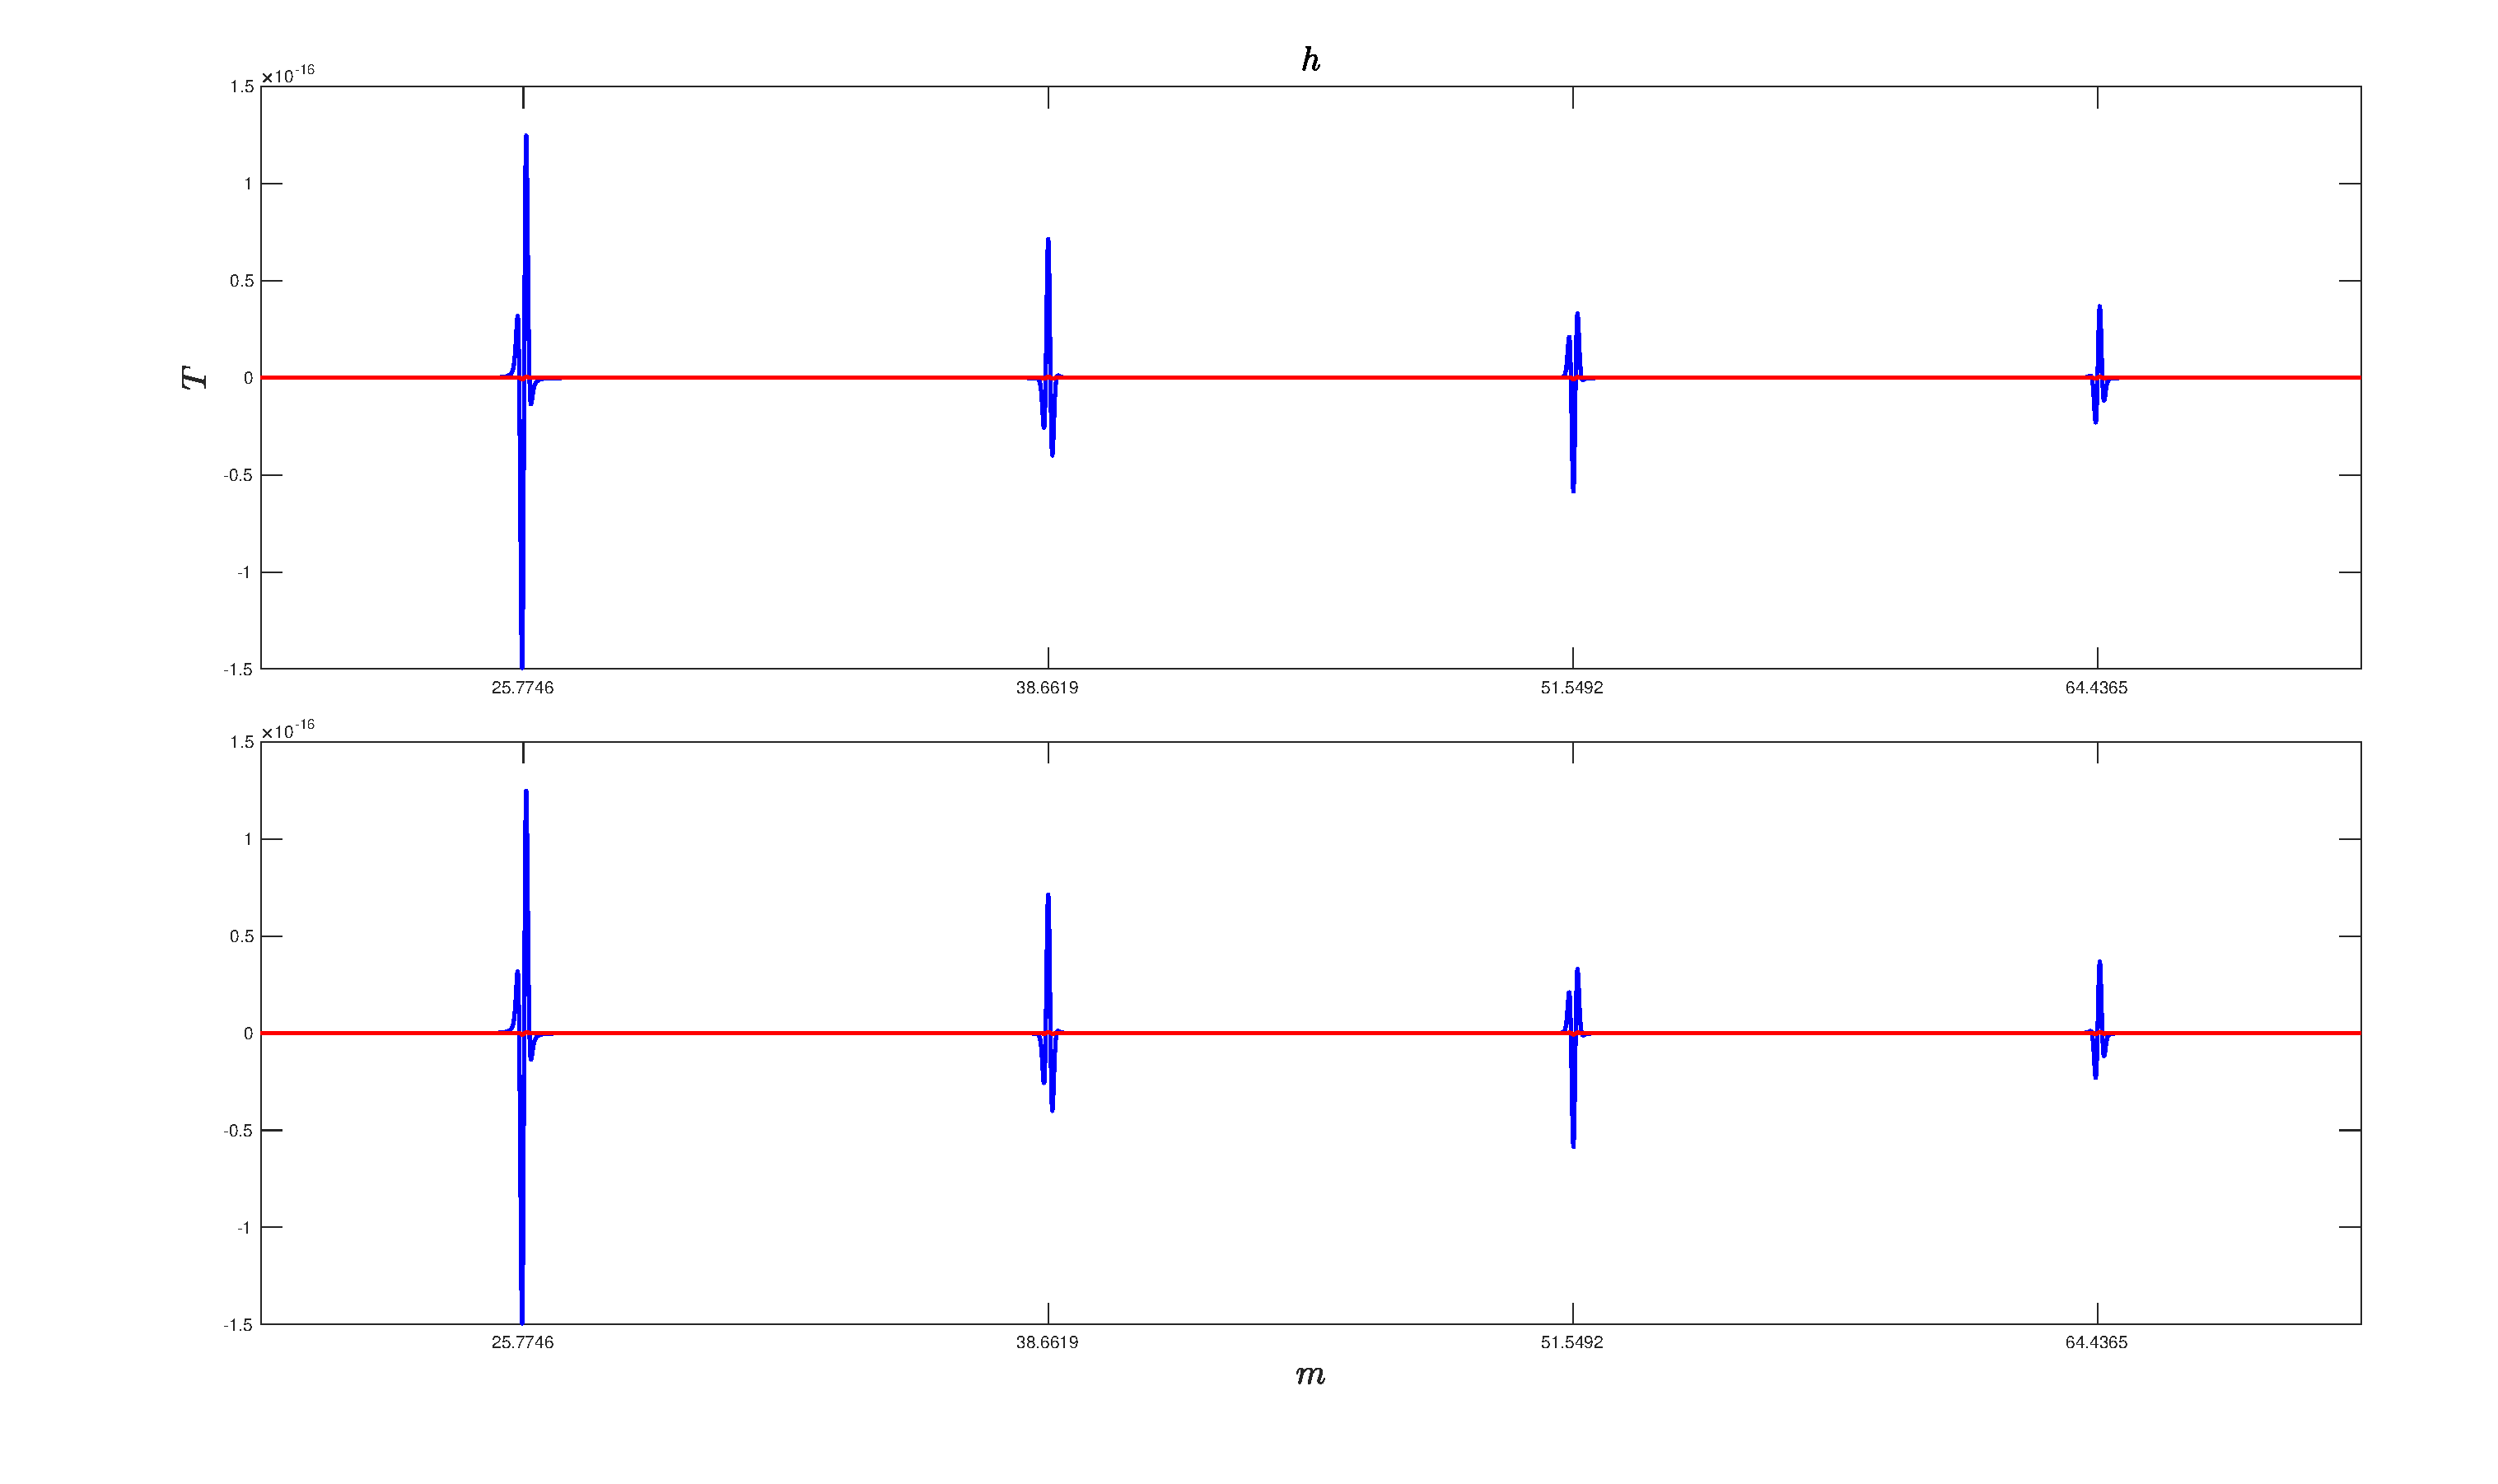
\includegraphics[scale=.5]{h_homo_F}
\caption{\textit{Tra\c{c}o s\'ismico do campo magn\'etico para sistema totalmente acoplado em cima e parcialmente acoplado embaixo, para pequenas dist\^ancias fonte/receptor.}}
\label{fig.mech_homo_high_dep}
\end{figure}
\end{landscape}

\begin{landscape}
\begin{figure}
\centering
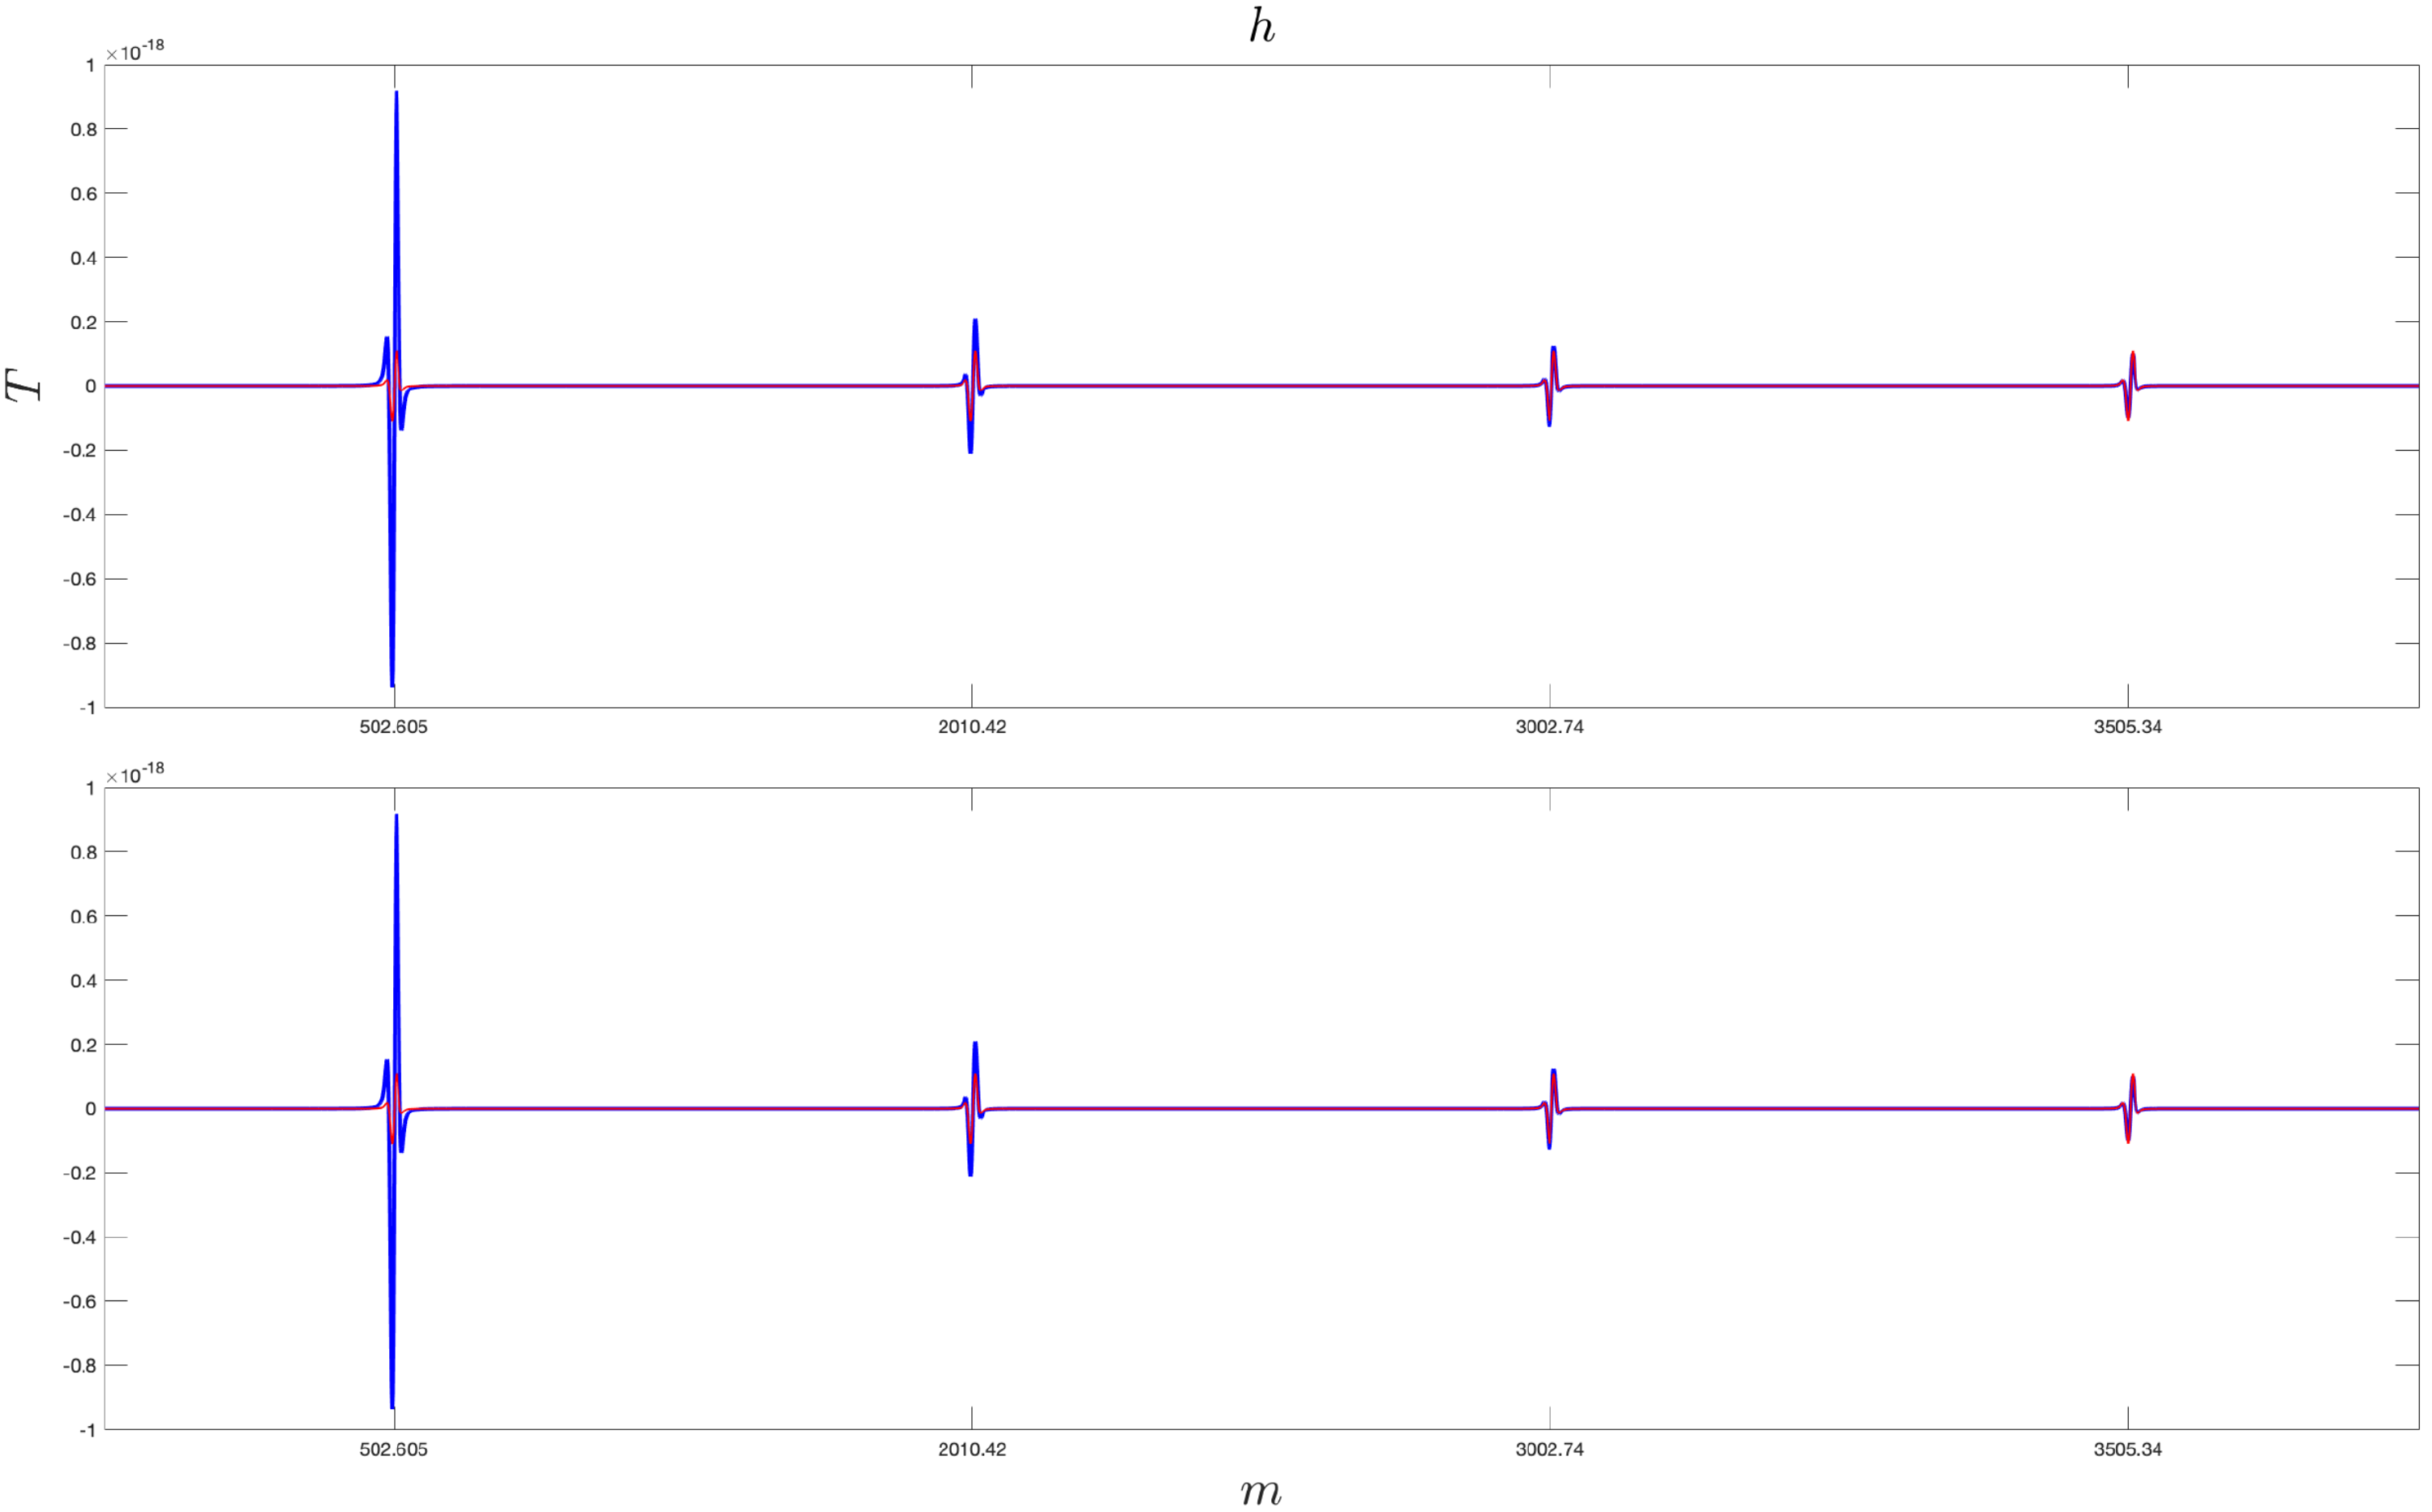
\includegraphics[scale=1.05]{h_homo_large_depth}
\caption{\textit{Tra\c{c}o s\'ismico do campo magn\'etico para sistema totalmente acoplado em cima e parcialmente acoplado embaixo, para grandes dist\^ancias fonte/receptor.}}
\label{fig.mag_homo_high_dep}
\end{figure}
\end{landscape}

\section{Ondas em Meio Estratificado se Propagando em uma Dimens\~ao}\label{sec.prop_strat_1D}

\subsection{Acoplamento Total}\label{sec.1D_four_fully}

Partindo das EDO's (\ref{eq.edo_2}), (\ref{eq.edo_3}), (\ref{eq.edo_7}) e (\ref{eq.edo_10}), vamos incluir a for\c{c}a de Lorentz dada pela equa\c{c}\~ao TAL na equa\c{c}\~ao (\ref{eq.edo_10}), para trabalharmos em um modelo com acoplamento total entre campos mec\^anicos e eletromagn\'eticos. Assim, temos o seguinte sistema
\begin{align*}
\frac{\partial\,E}{\partial\,z}&=-i\,\omega\,\mu_0\,h\\\\
\frac{\partial\,h}{\partial\,z}&=\sigma\,E-i\,\omega\,\sigma\,\mu_0h^0u\\\\
\frac{\partial\,u}{\partial\,z}&=\frac{1}{\lambda+2\,G}\,\tau\\\\
\frac{\partial\,\tau}{\partial\,z}&=-\omega^2\,\rho\,u+\mu_0h^0\frac{\partial\,h}{\partial\,z}-F.
\end{align*}
Seguindo o algoritmo em formato matricial preconizado por \cite{ursin-1983}, temos
\begin{equation}\label{eq.four_f_full_coupled_1D_model}
\frac{\partial}{\partial\,z}\begin{pmatrix}
h\\
\tau\\
E\\
u
\end{pmatrix}
=
-i\,\omega\begin{pmatrix}
0&0&\frac{-\sigma}{i\,\omega}&\sigma\,\mu_0h^0\\
0&0&\frac{-\sigma\,\mu_0h^0}{i\,\omega}&\sigma\,\mu_0^2(h^0)^2-i\,\omega\rho\\
\mu_0&0&0&0\\
0&\frac{-1}{i\,\omega\,(\lambda+2\,G)} &0&0
\end{pmatrix}
\begin{pmatrix}
h\\
\tau\\
E\\
u
\end{pmatrix}
+
\begin{pmatrix}
0\\
-F\\
0\\
0
\end{pmatrix}.
\end{equation}
\begin{equation*}
M_1M_2=\begin{pmatrix}
\frac{\sigma\,\mu_0}{-i\,\omega}&\frac{-\sigma\,\mu_0h^0}{i\,\omega\,(\lambda+2\,G)}\\\\
\frac{\sigma\,\mu_0^2h^0}{-i\,\omega}&\frac{i\,\omega\rho-\sigma\,\mu_0^2(h^0)^2}{i\,\omega\,(\lambda+2\,G)}
\end{pmatrix}
=\begin{pmatrix}
m_{11}&m_{12}\\
m_{21}&m_{22}
\end{pmatrix}.
\end{equation*}
Sendo $q^2_{1,2}$ os autovalores para a matriz $M_1M_2$, temos que os autovetores s\~ao dados por
\begin{equation*}
\mathbf{a}_1=\begin{pmatrix}
a_1\\\\
\frac{q_1^2-m_{11}}{m_{12}}\,a_1
\end{pmatrix}\qquad\text{e}\qquad
\mathbf{a}_2=\begin{pmatrix}
\frac{m_{12}}{q_2^2-m_{11}}\,a_2\\\\
a_2
\end{pmatrix},
\end{equation*}
onde
\begin{equation*}
a_1=\sqrt{\frac{q_1}{\mu_0-\frac{(q_1^2-m_{11})^2}{i\,\omega\,m_{12}^2(\lambda+2\,G)}}}\qquad\text{e}\qquad 
a_2=\sqrt{\frac{q_2}{\frac{m_{12}^2\mu_0}{(q_2^2-m_{11})^2}-\frac{1}{i\,\omega\,(\lambda+2\,G)}}}.
\end{equation*}
Os autovalores para a matriz $M_2M_1$ tamb\'em s\~ao dados por $q_{1,2}^2$, e os autovetores s\~ao
\begin{equation*}
\mathbf{b}_1=\frac{1}{q_1}\begin{pmatrix}
\mu_0a_1\\\\
\frac{q_1^2-m_{11}}{-i\,\omega\,m_{12}(\lambda+2\,G)}\,a_1
\end{pmatrix}\qquad\text{e}\qquad
\mathbf{b}_2=\frac{1}{q_2}\begin{pmatrix}
\frac{\mu_0m_{12}}{q_2^2-m_{11}}\,a_2\\\\
\frac{1}{-i\,\omega\,(\lambda+2\,G)}a_2
\end{pmatrix}.
\end{equation*}
Vamos utilizar uma fonte n\~ao causal que simula a aplica\c{c}\~ao de uma for\c{c}a vertical dada por
\begin{equation*}
F=\delta(z-z_0)\,rck(\omega),
\end{equation*}
onde $\delta$ de \textit{Dirac} \'e a fun\c{c}\~ao dada pela subse\c{c}\~ao (\ref{sec.dirac}) e $rck(\omega)$ \'e o pulso de \textit{Ricker} no dom\'inio da frequ\^encia angular. Seguindo a subse\c{c}\~ao \ref{sec.presenca_fonte}, vamos substituir $F$ na fonte $\mathbf{S}$ e usar a rela\c{c}\~ao
\begin{equation*}
\mathbf{S}=\delta(z-z_0)\,\begin{pmatrix}
\mathbf{S_A}\\
\mathbf{S_B}
\end{pmatrix},
\end{equation*}
para obtermos
\begin{equation*}
\mathbf{S_A}=\begin{pmatrix}
0\\
rck
\end{pmatrix}\qquad\text{e}\qquad\mathbf{S_B}=\begin{pmatrix}
0\\
0
\end{pmatrix}.
\end{equation*}
As condi\c{c}\~oes de contorno s\~ao inseridas usando as matrizes $G_A$ e $G_B$, conforme a subse\c{c}\~ao \ref{sec.cond_contorno},
\begin{equation*}
\mathbf{\Phi}=\begin{pmatrix}
G_A\\
G_B
\end{pmatrix}\mathbf{\Phi}_g,
\end{equation*}
onde
\begin{equation*}
G_A=\begin{pmatrix}
\frac{q_0}{\mu_0}&0\\
0&0
\end{pmatrix},\qquad G_B=\begin{pmatrix}
1&0\\
0&1
\end{pmatrix}\qquad\text{e}\qquad\mathbf{\Phi}_g=\begin{pmatrix}
E\\
u
\end{pmatrix}.
\end{equation*}
Assim, podemos obter numericamente as solu\c{c}\~oes para o sistema (\ref{eq.four_f_full_coupled_1D_model}), em que duas delas t\^em seus gr\'aficos nas figuras (\ref {fig.four_fully_1D_u}) e (\ref{fig.four_fully_1D_h}), onde podemos observar, respectivamente, o campo mec\^anico e o campo magn\'etico de ondas que se propagam em camadas estratigr\'aficas. Para esta simula\c{c}\~ao estamos considerando uma geometria estratigr\'afica com duas camadas onde a camada 1 tem a superf\'icie livre de contato com o ar e tem $1000\,m$ de profundidade. A camada 1, que \'e onde ocorre a propaga\c{c}\~ao, forma uma interface de contato com a camada 2 a qual possui profundidade infinita, e as caracter\'sticas dessas camadas est\~ao na tabela (\ref{tab.dados_propagacao}). Tanto na figura  (\ref {fig.four_fully_1D_u}) como na figura (\ref{fig.four_fully_1D_h}) podemos visualizar nitidamente tr\^es eventos para a onda mec\^anica e eletromagn\'etica, respectivamente. Nesses dois gr\'aficos temos a chegada de uma onda direta no tempo zero (simulando com fonte n\~ao causal e receptor na mesma posi\c{c}\~ao), seguida de uma reflex\~ao na interface entre a primeira e segunda camadas, e por \'ultimo uma m\'ultipla da referida reflex\~ao. A interface est\'a a 1000 $m$ de profundidade em rela\c{c}\~ao \`a superficie livre onde est\'a a fonte, e observamos que a m\'ultipla tem o dobro do tempo de chegada em rela\c{c}\~ao \`a sua correspondente reflex\~ao, para ambas as ondas. Como estamos trabalhando com modelo de acoplamento entre as ondas, o tempo de chegada da reflex\~ao da onda mec\^anica \'e bastante pr\'oximo do tempo da onda eletromagn\'etica, e o tempo de chegada tamb\'em \'e similar entre as m\'ultiplas dessas duas ondas.

\begin{figure}
\centering
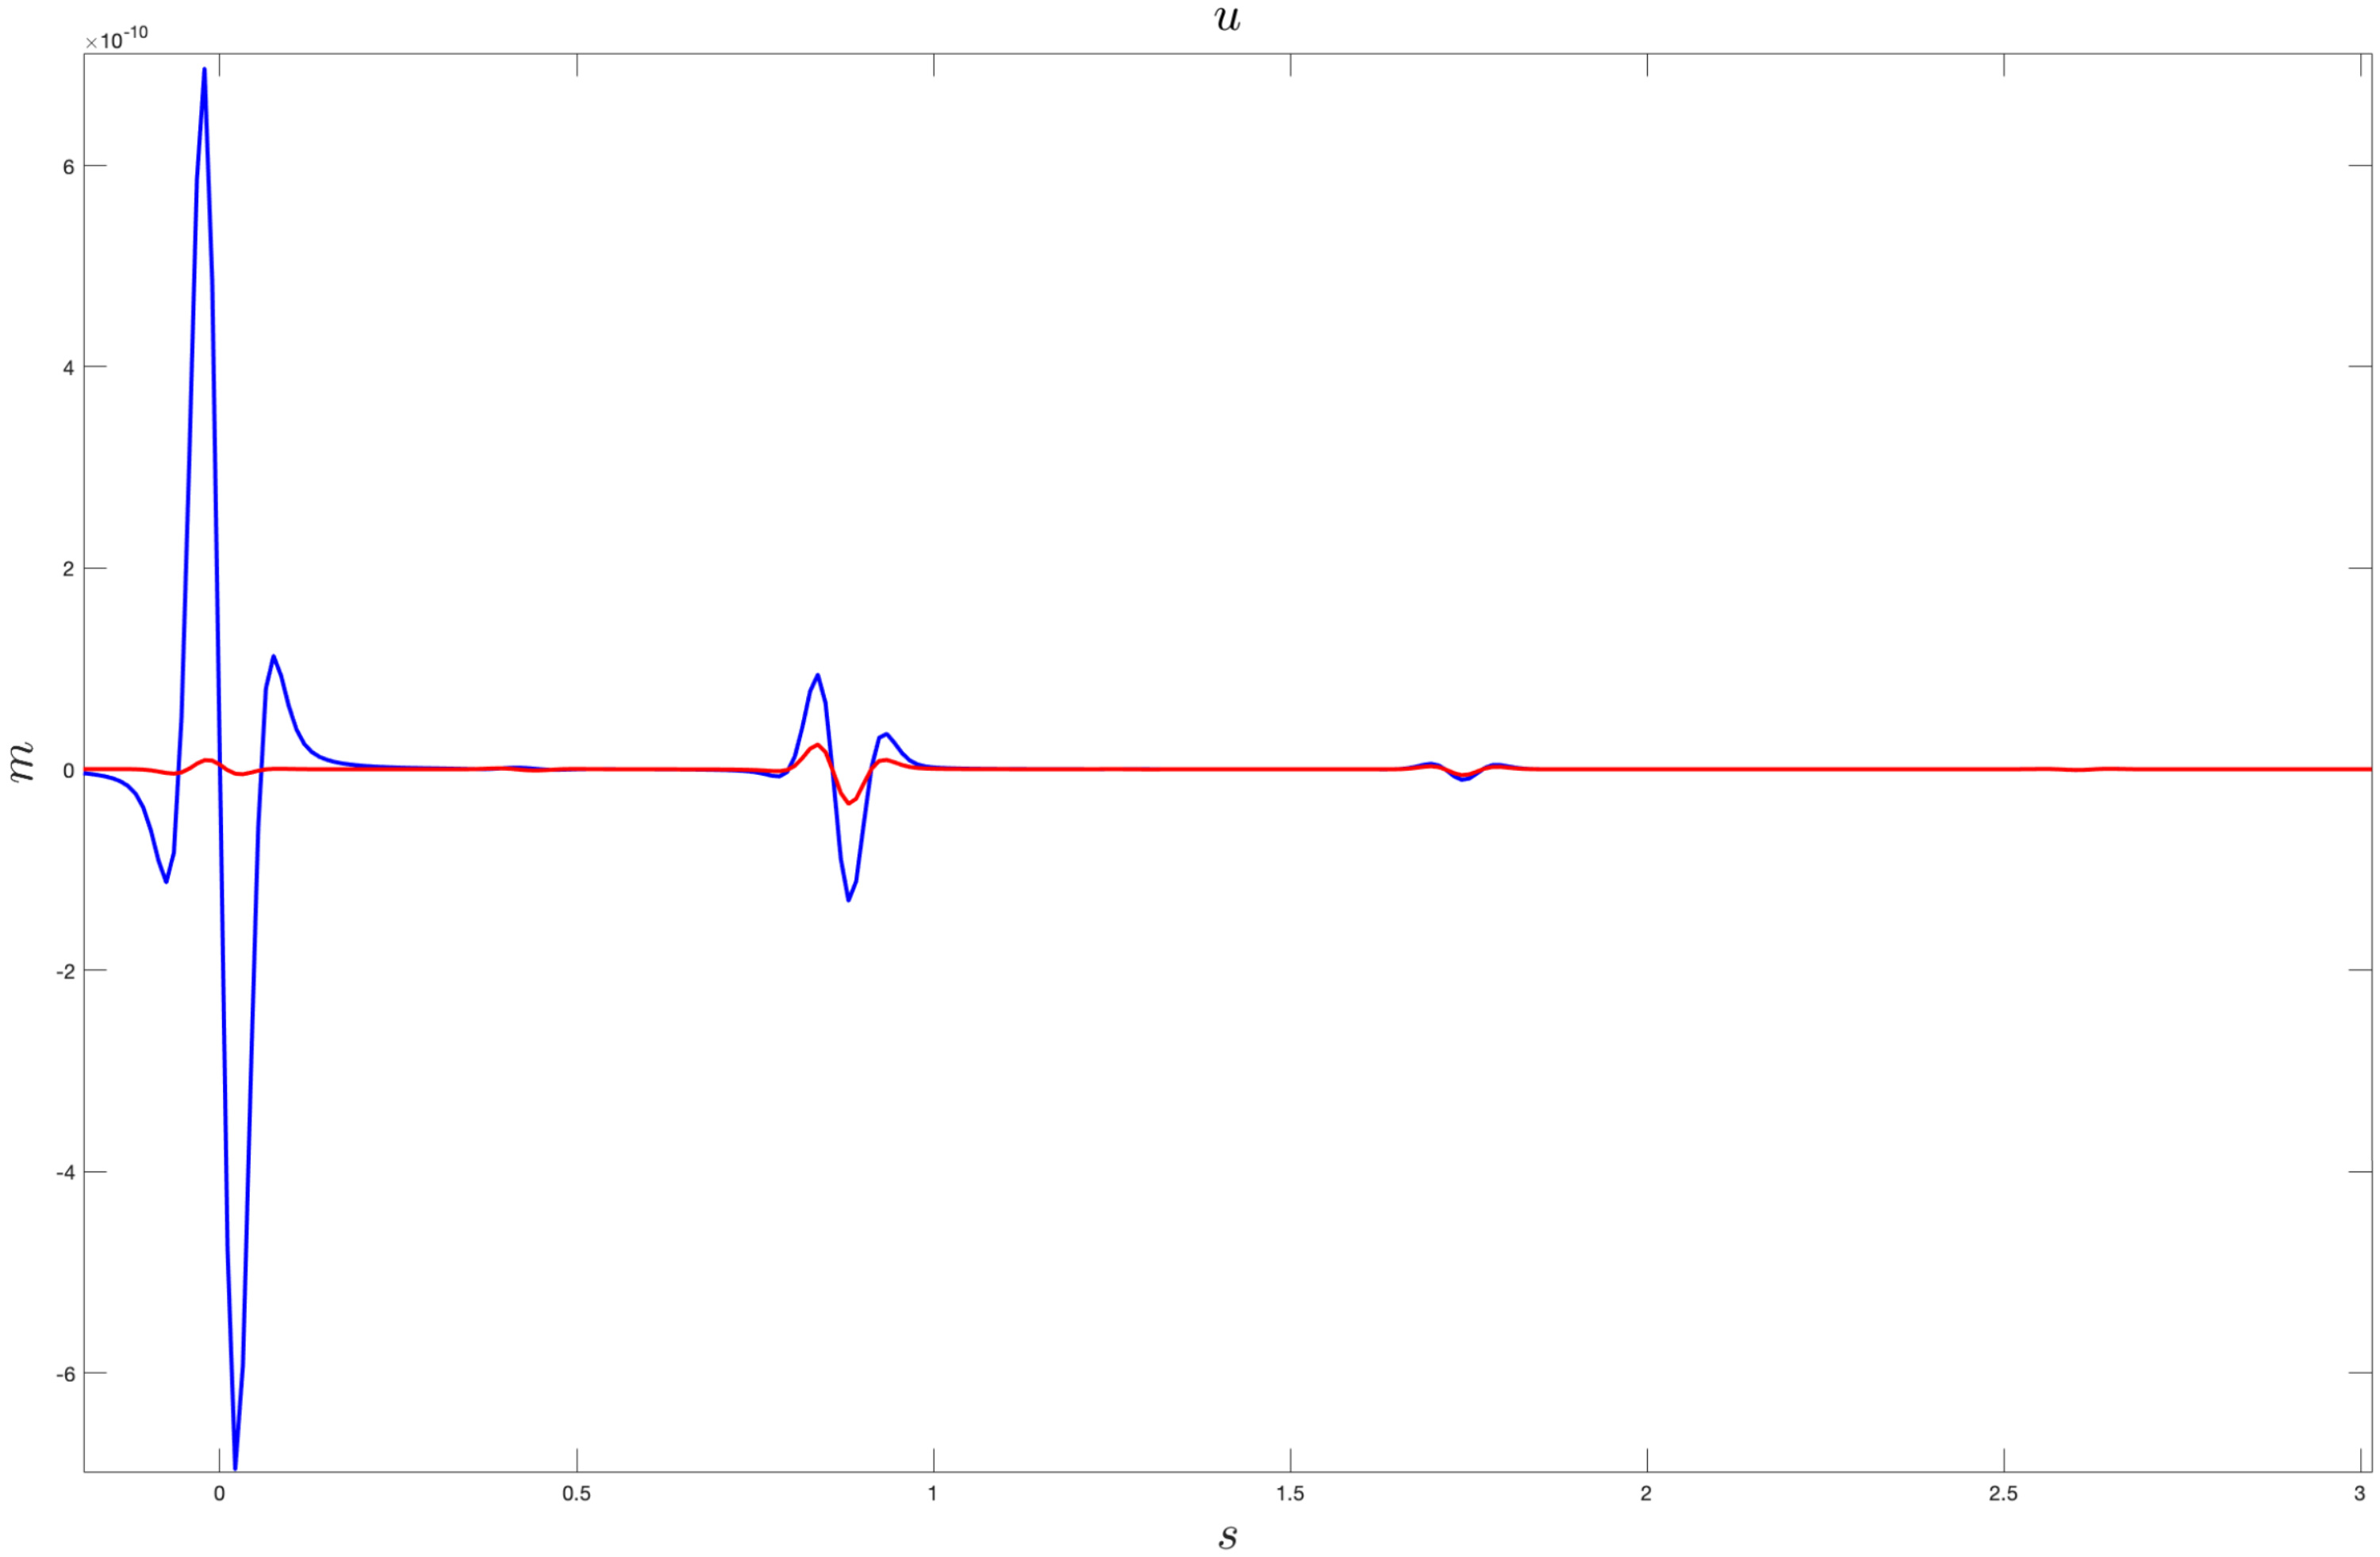
\includegraphics[scale=.9]{four_fully_1D_u}\\
\caption{\textit{Campo mec\^anico em acoplamento total, com fonte e receptor na superf\'icie e interface a 1000 $m$. Observamos a onda direta, seguida da reflex\~ao e depois uma m\'ultipla.}}
\label{fig.four_fully_1D_u}
\end{figure}


\begin{figure}
\centering
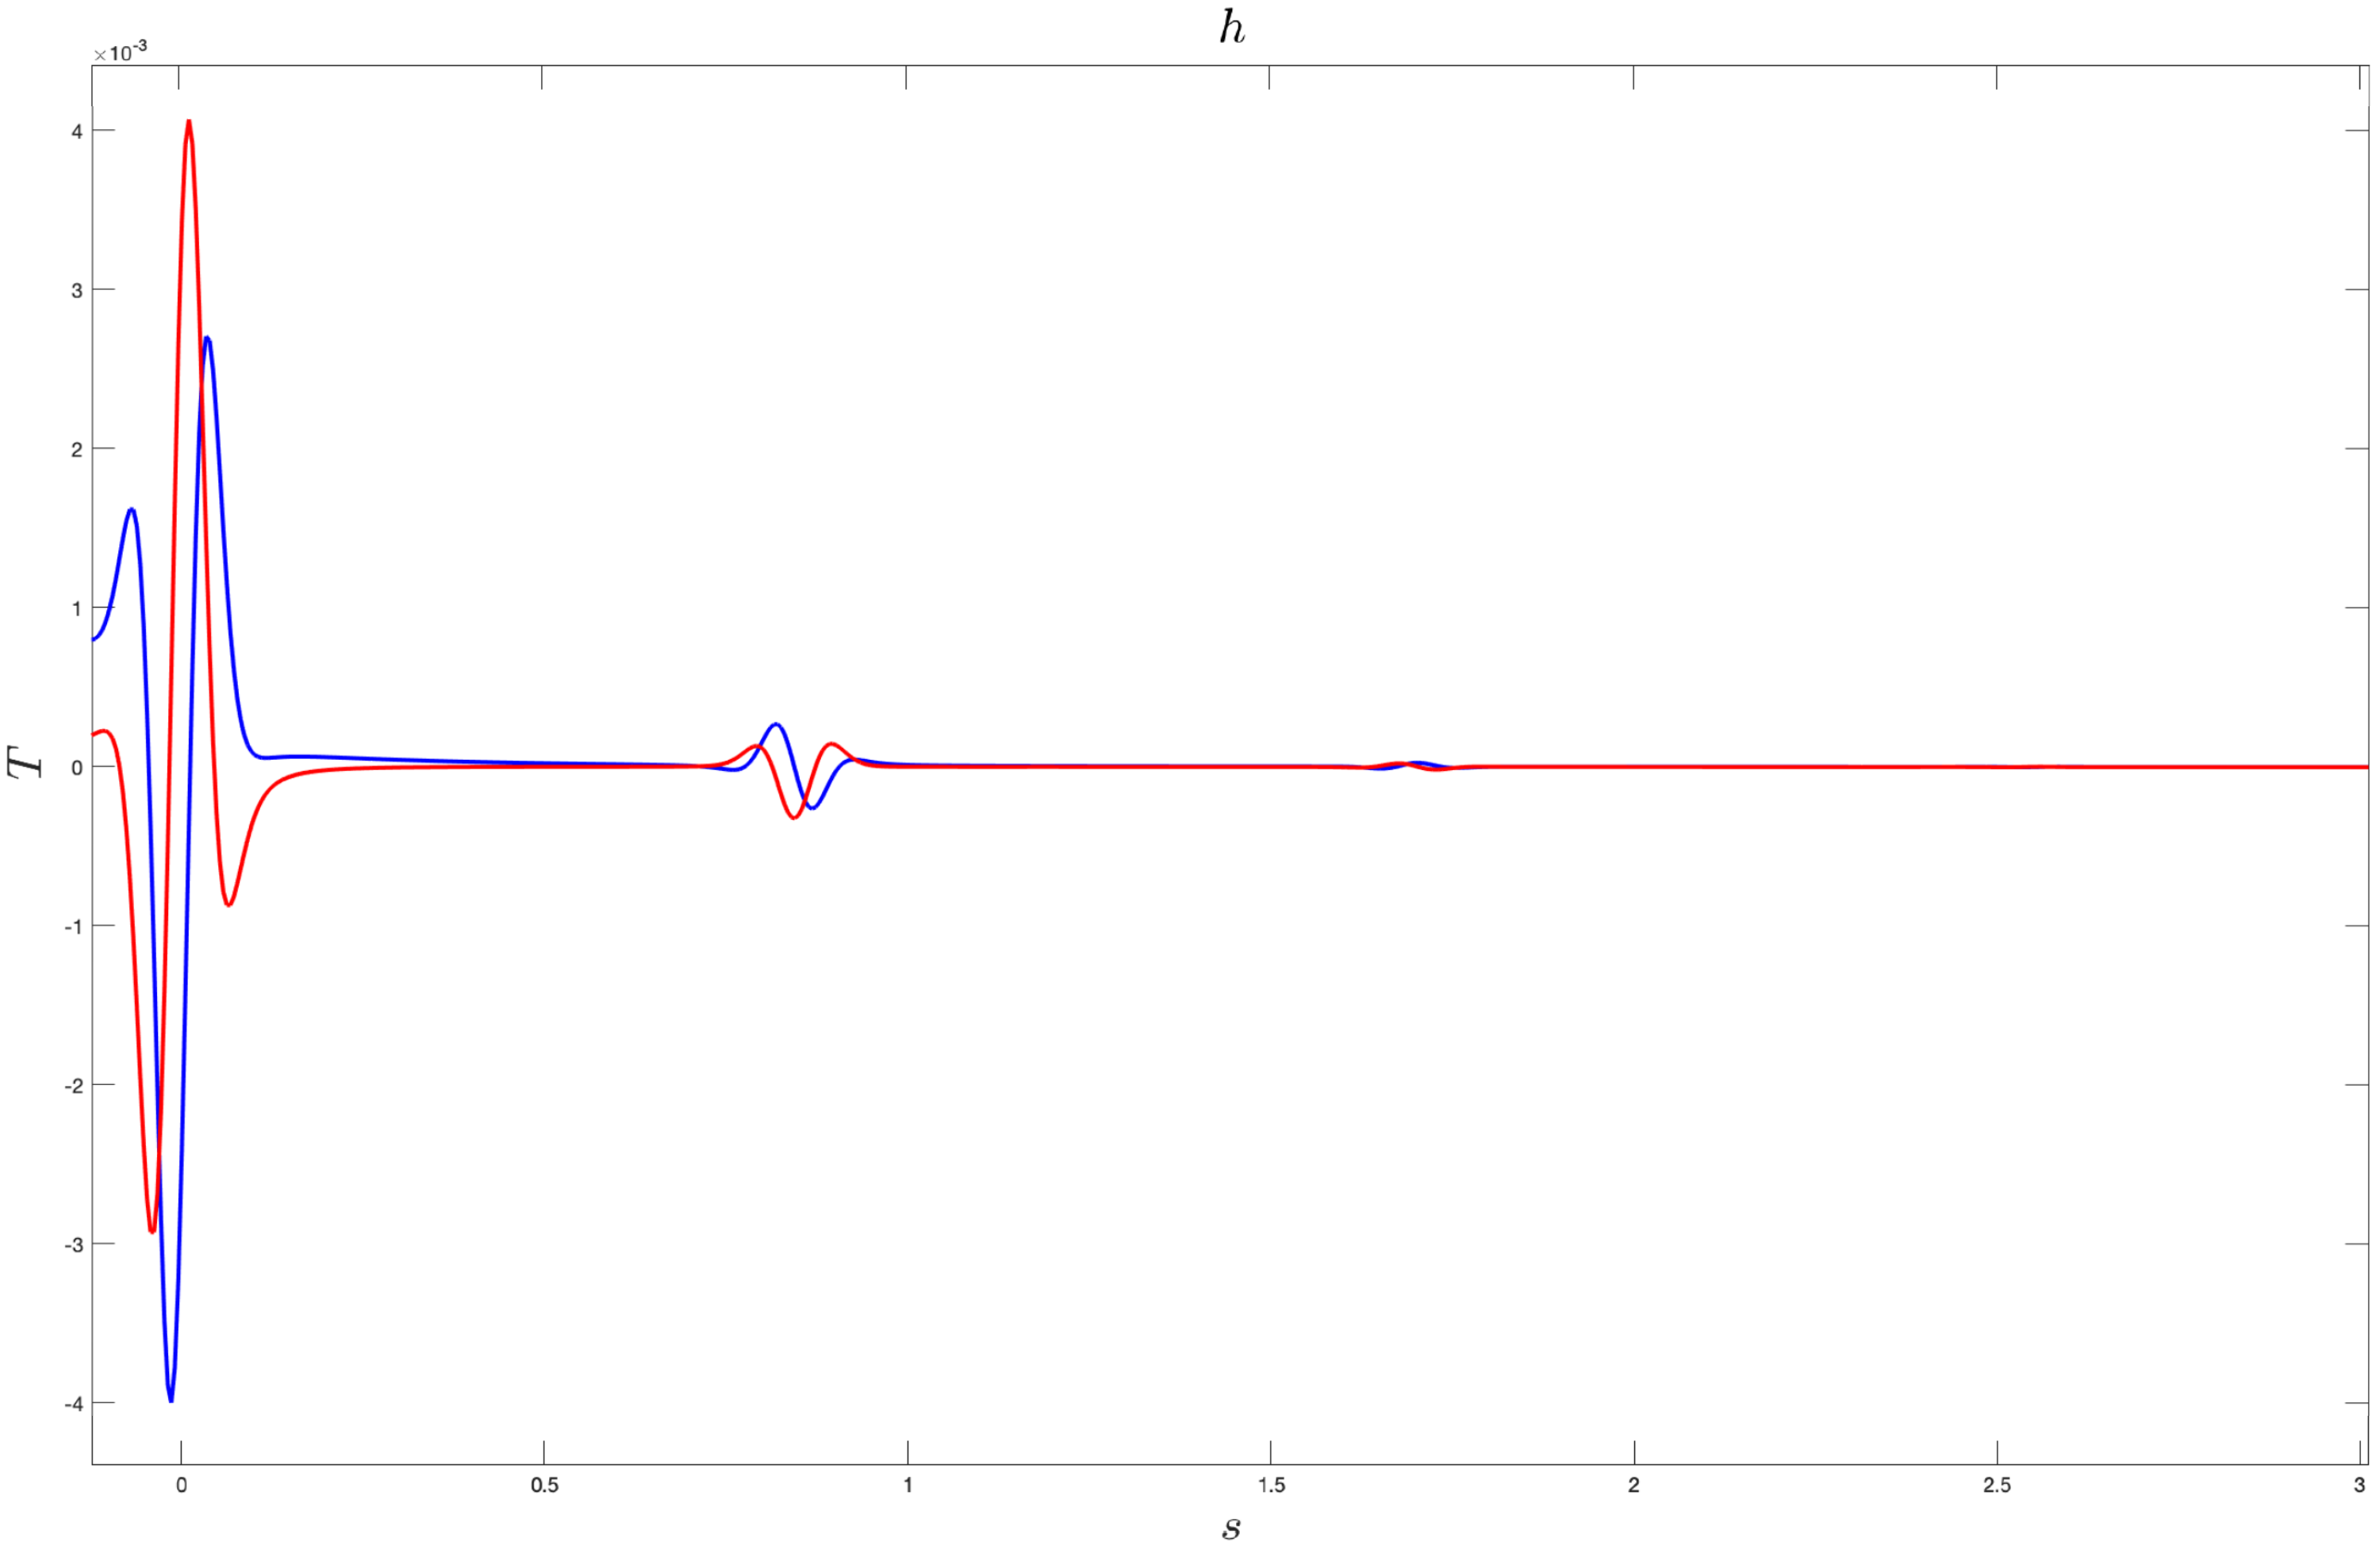
\includegraphics[scale=.825]{four_fully_1D_h}\\
\caption{\textit{Campo magn\'etico em acoplamento total, com fonte e receptor na superf\'icie e interface a 1000 $m$. Observamos a onda direta, seguida da reflex\~ao e depois uma m\'ultipla.}}
\label{fig.four_fully_1D_h}
\end{figure}


\subsection{Acoplamento Parcial}
Para tratarmos do acoplamento parcial, vamos desconsiderar a influ\^encia que os campos eletromagn\'eticos exercem sobre os campos mec\^anicos, ou seja, o modelo dado pelas equa\c{c}\~oes \ref{eq.four_f_full_coupled_1D_model} \'e reescrito como
\begin{equation*}
\frac{\partial}{\partial\,z}\begin{pmatrix}
h\\
\tau\\
E\\
u
\end{pmatrix}
=
-i\,\omega\begin{pmatrix}
0&0&\frac{-\sigma}{i\,\omega}&\sigma\,\mu_0h^0\\
0&0&0&\sigma\,\mu_0^2(h^0)^2-i\,\omega\rho\\
\mu_0&0&0&0\\
0&\frac{-1}{i\,\omega\,(\lambda+2\,G)} &0&0
\end{pmatrix}
\begin{pmatrix}
h\\
\tau\\
E\\
u
\end{pmatrix}
+
\begin{pmatrix}
0\\
-F\\
0\\
0
\end{pmatrix},
\end{equation*}
e a matriz $M_1M_2$ passa a ser dada por
\begin{equation*}
M_1M_2=\begin{pmatrix}
\frac{\sigma\,\mu_0}{-i\,\omega}&\frac{-\sigma\,\mu_0h^0}{i\,\omega\,(\lambda+2\,G)}\\\\
0&\frac{i\,\omega\rho-\sigma\,\mu_0^2(h^0)^2}{i\,\omega\,(\lambda+2\,G)}
\end{pmatrix}
=\begin{pmatrix}
m_{11}&m_{12}\\
m_{21}&m_{22}
\end{pmatrix}.
\end{equation*}
Os autovalores e autovetores, fonte e condi\c{c}\~oes de contorno para esse novo modelo podem ser calculados usando as mesmas f\'ormulas da subse\c{c}\~ao \ref{sec.1D_four_fully}, bastando tomar $m_{21}=0$ para determinarmos os autovalores. As solu\c{c}\~oes podem ser observadas nas figuras (\ref{fig.four_partially_1D_mech}) e (\ref{fig.four_partially_1D_eletro}).

\begin{figure}
\centering
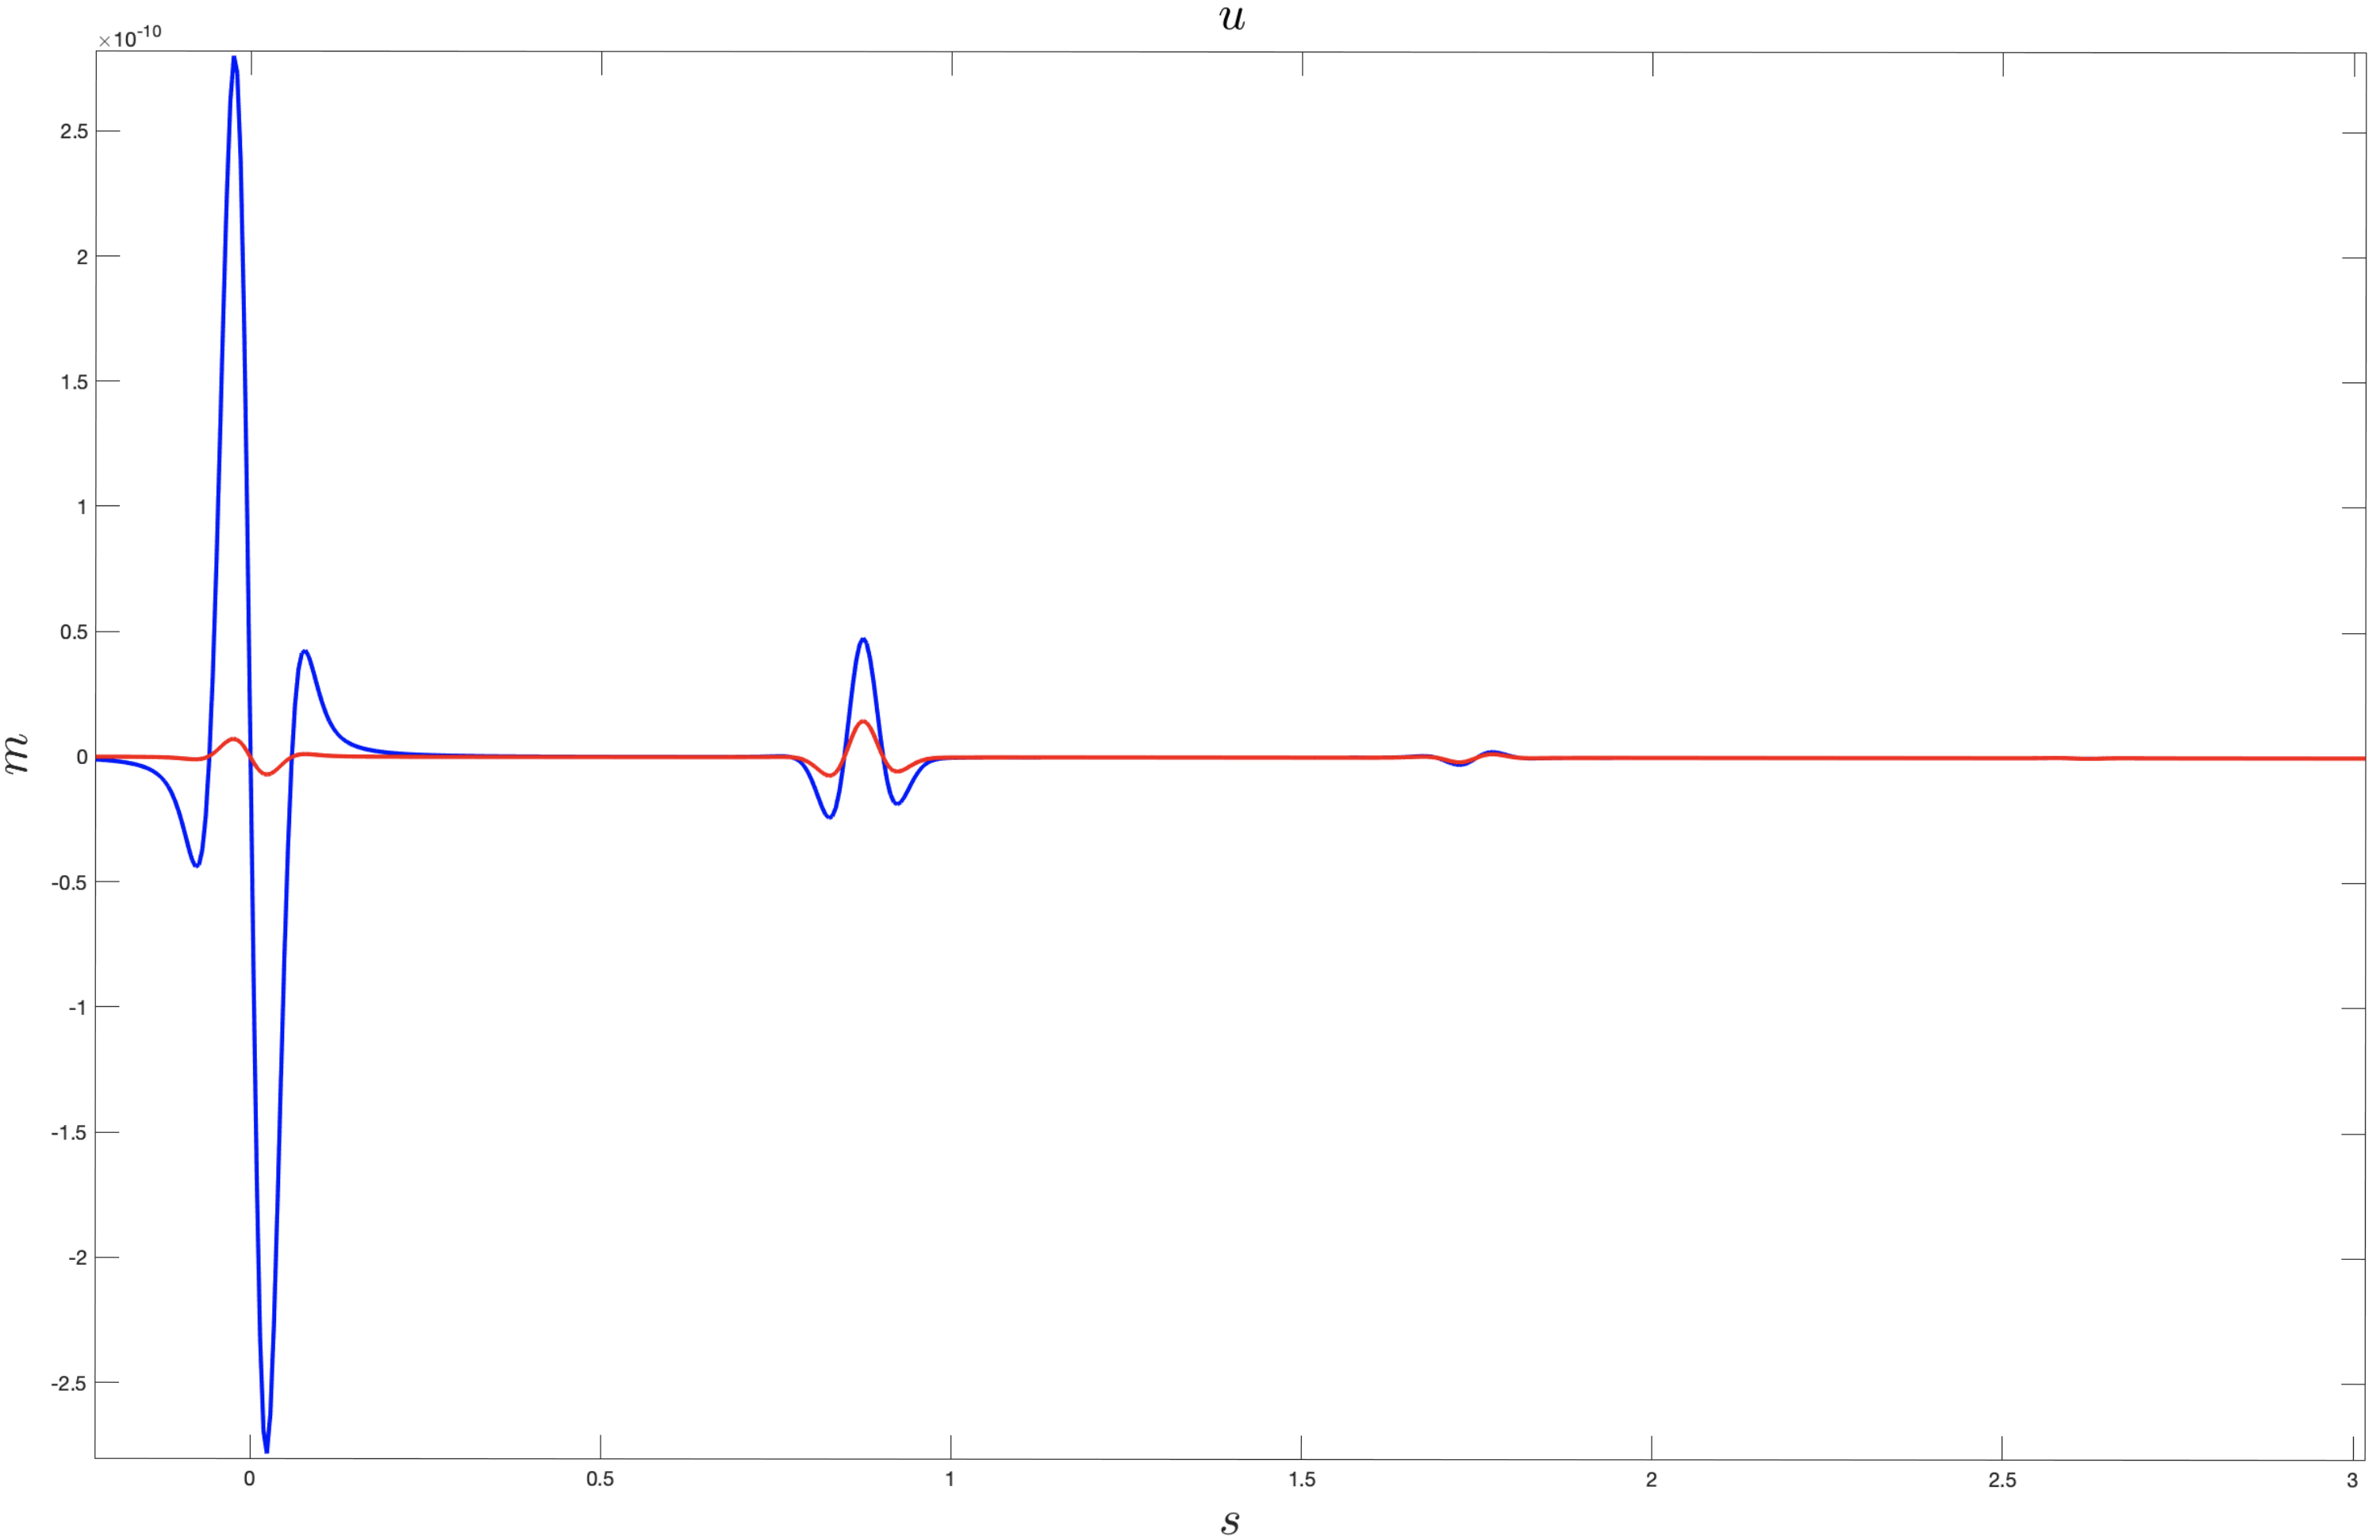
\includegraphics[scale=.71]{four_partially_1D_u}\\
\caption{\textit{Podemos observar a chegada da onda direta seguida de uma reflex\~ao e uma m\'ultipla de uma onda mec\^anica, num sistema parcialmente acoplado.}}
\label{fig.four_partially_1D_mech}
\end{figure}

\begin{figure}
\centering
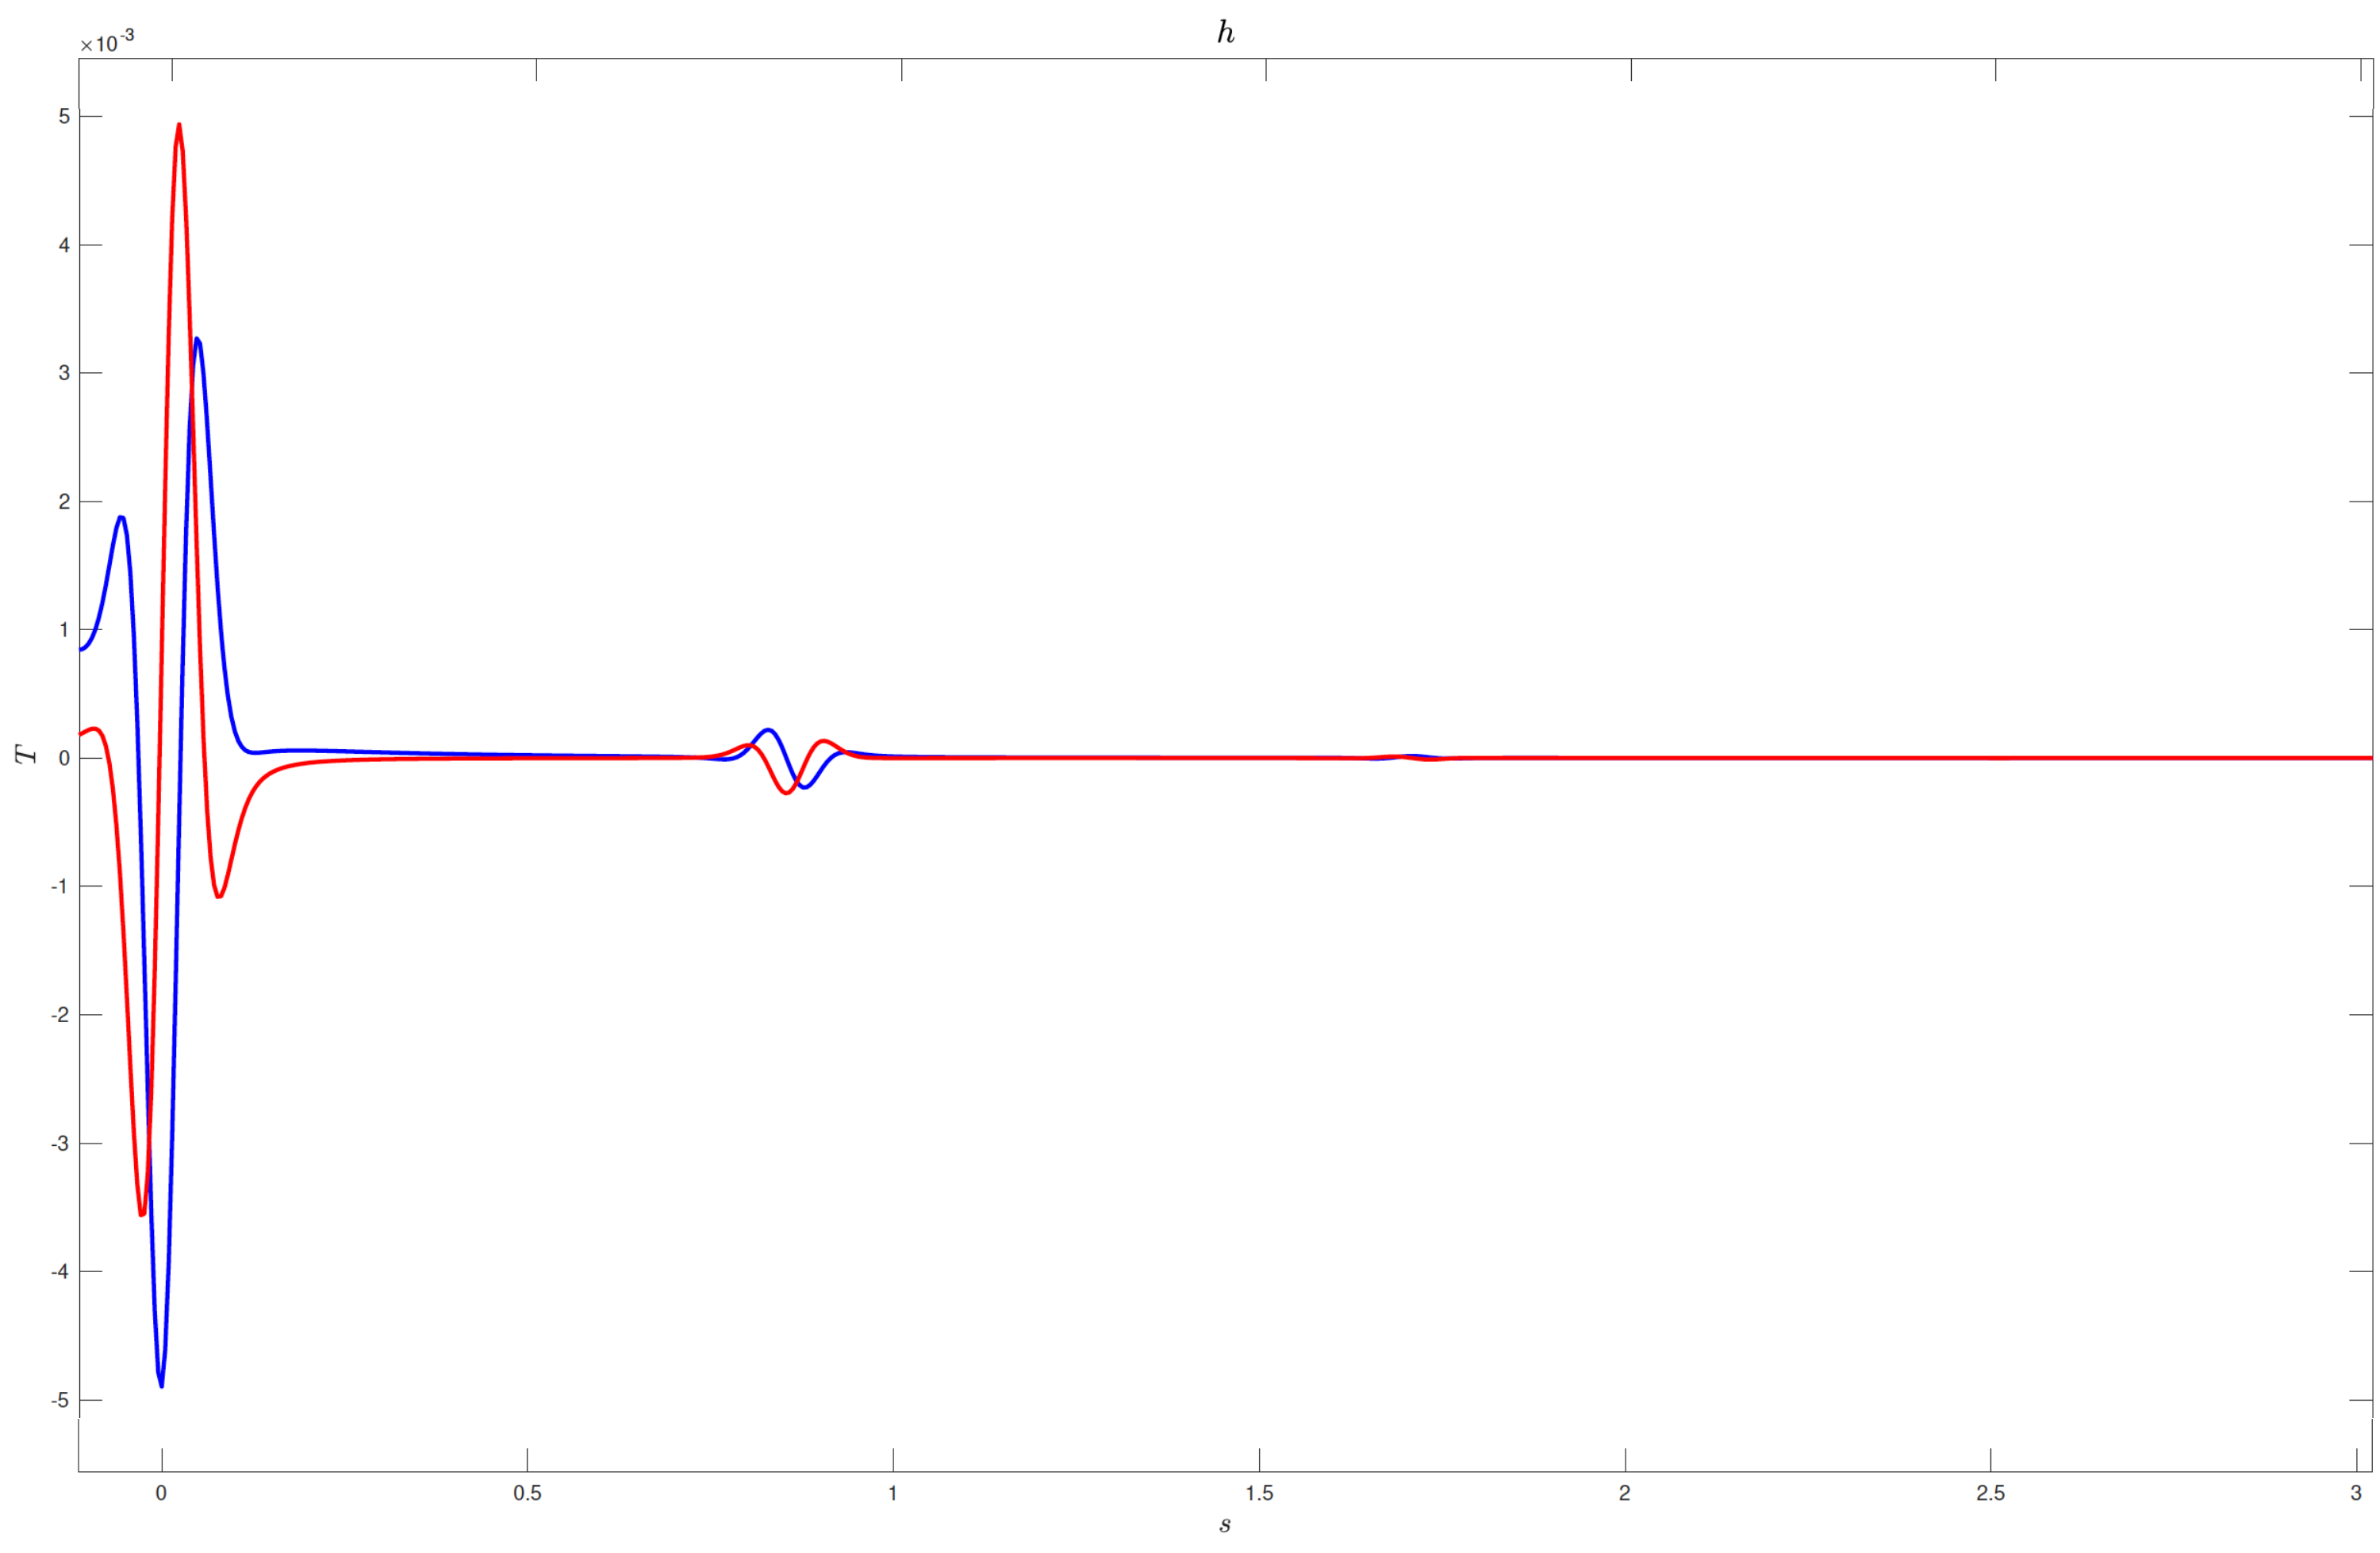
\includegraphics[scale=.85]{four_partially_1D_h}\\
\caption{\textit{Onda direta seguida de uma reflex\~ao e uma m\'ultipla (de amplitude bem pequena) de uma onda eletromagn\'etica, num sistema parcialmente acoplado.}}
\label{fig.four_partially_1D_eletro}
\end{figure}

Comparando os campos mec\^anicos do modelo de acoplamento total na figura (\ref{fig.four_fully_1D_u}) com o modelo de acoplamento parcial na figura (\ref{fig.four_partially_1D_mech}), observamos que n\~ao houve altera\c{c}\~ao significativa na propaga\c{c}\~ao dessas ondas quando mudamos o modelo. Os tempos de chegada e as amplitudes das ondas diretas, das reflex\~oes na primeira interface e das respectivas m\'ultiplas, permanecem aproximadamente iguais. Quaisquer discrep\^ancias entre os gr\'aficos podem estar relacionadas \`a estabilidade num\'erica, j\'a que para o caso parcialmente acoplado estamos computando uma quantidade menor de dados e, consequentemente, seu gr\'afico pode apresentar menos ru\'ido e sinais de instabilidade. 

Vamos mudar algumas caracter\'isticas da segunda camada para alterarmos a rela\c{c}\~ao de imped\^ancia e o coeficiente de reflex\~ao entre a primeira e segunda camadas para uma melhor visualiza\c{c}\~ao dos eventos. Em rela\c{c}\~ao \`a tabela (\ref{tab.dados_propagacao}), alteramos a segunda camada para $\rho=3000\,\frac{kg}{m^3}$ e $\sigma=1\,S/m$ (uma caracter\'istica mec\^anica e uma eletromagn\'etica), e com isso conseguimos uma melhor visualiza\c{c}\~ao da reflex\~ao e das m\'ultiplas na figura (\ref{fig.four_partially_1D_mech_hi_ampl}) para onda mec\^anica e na figura (\ref{fig.four_partially_1D_electro_hi_ampl}) para onda eletromagn\'etica. Comparando as figuras (\ref{fig.four_partially_1D_mech}) e (\ref{fig.four_partially_1D_mech_hi_ampl}), al\'em de termos  um aumento nas amplitudes da reflex\~ao e das m\'ultiplas, aumentamos tamb\'em a quantidade de m\'ultiplas vis\'iveis. Note ainda que o tempo de chegada da reflex\~ao e das m\'ultiplas n\~ao foram alterados, pois s\'o mudamos as caracter\'isticas da segunda camada e a onda mec\^anica est\'a se propagando na primiera. Essa mesma an\'alise pode ser aplicada \`a onda eletromagn\'etica comparando as figuras (\ref{fig.four_partially_1D_eletro}) e (\ref{fig.four_partially_1D_electro_hi_ampl}).

\begin{figure}
\centering
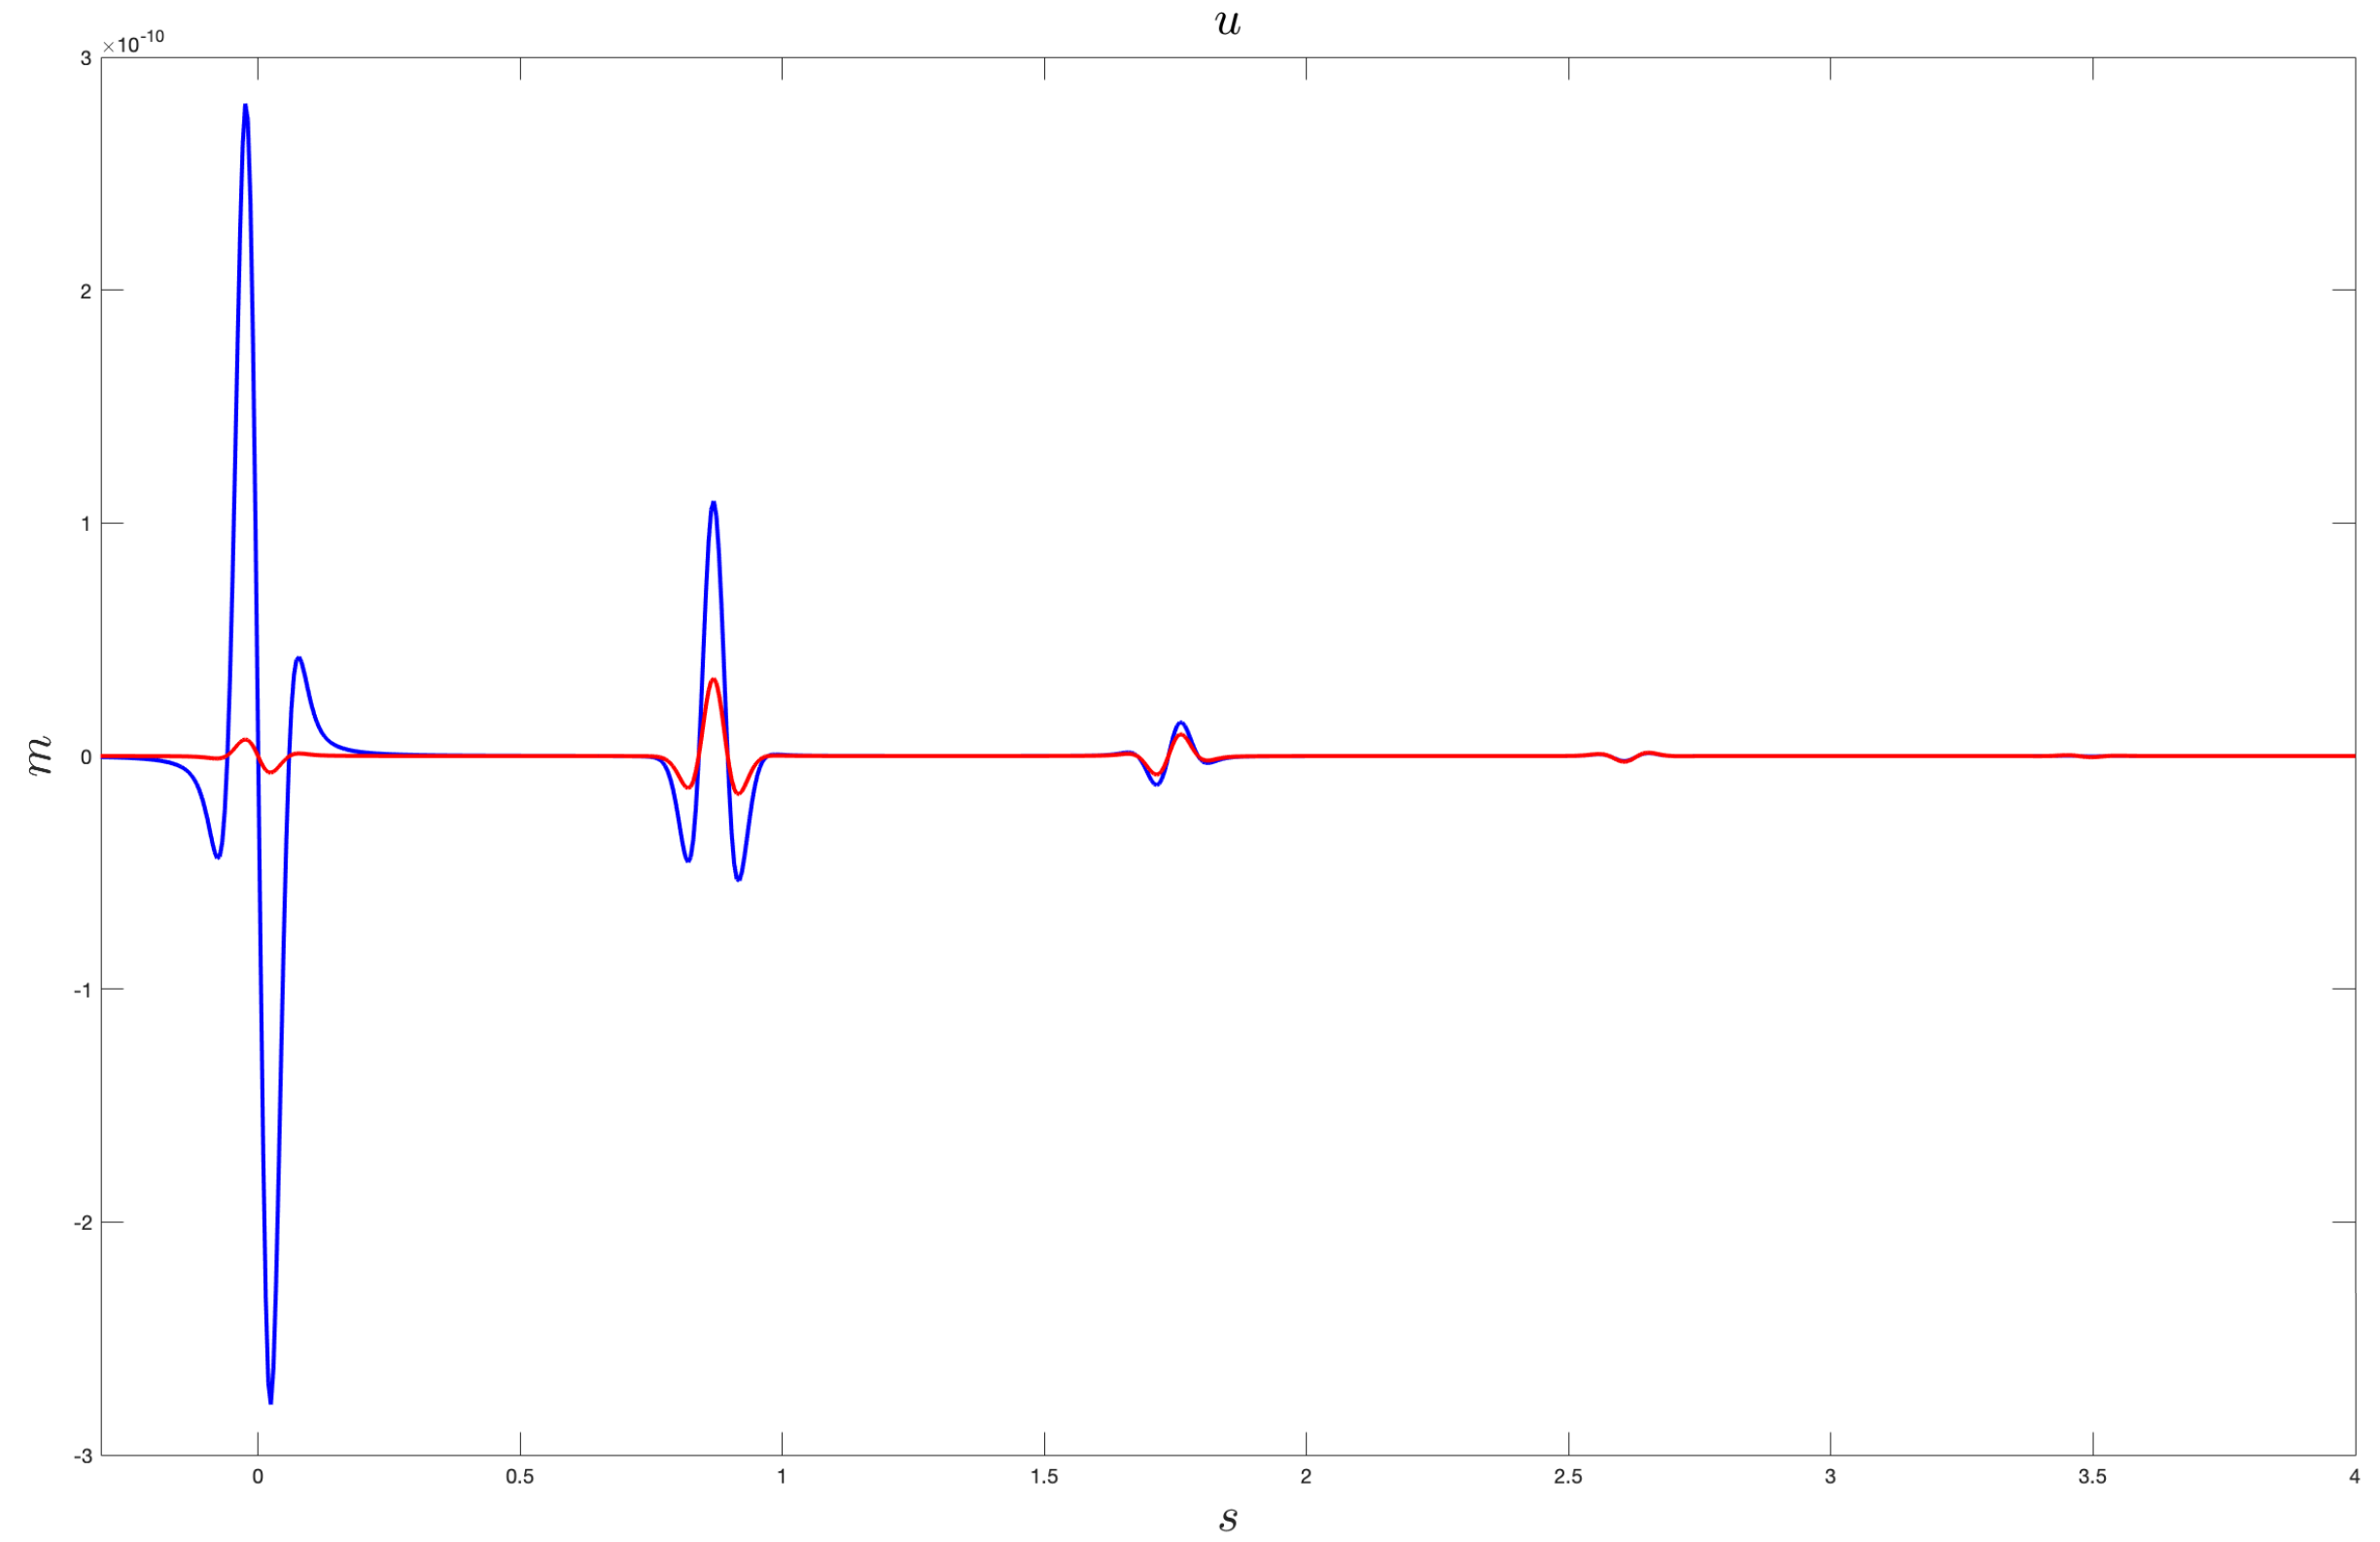
\includegraphics[scale=.36]{four_partially_1D_high_ampl_u}\\
\caption{\textit{Podemos observar a chegada da onda direta seguida de uma reflex\~ao e de tr\^es m\'ultiplas da onda mec\^anica.}}
\label{fig.four_partially_1D_mech_hi_ampl}
\end{figure}


\begin{figure}
\centering
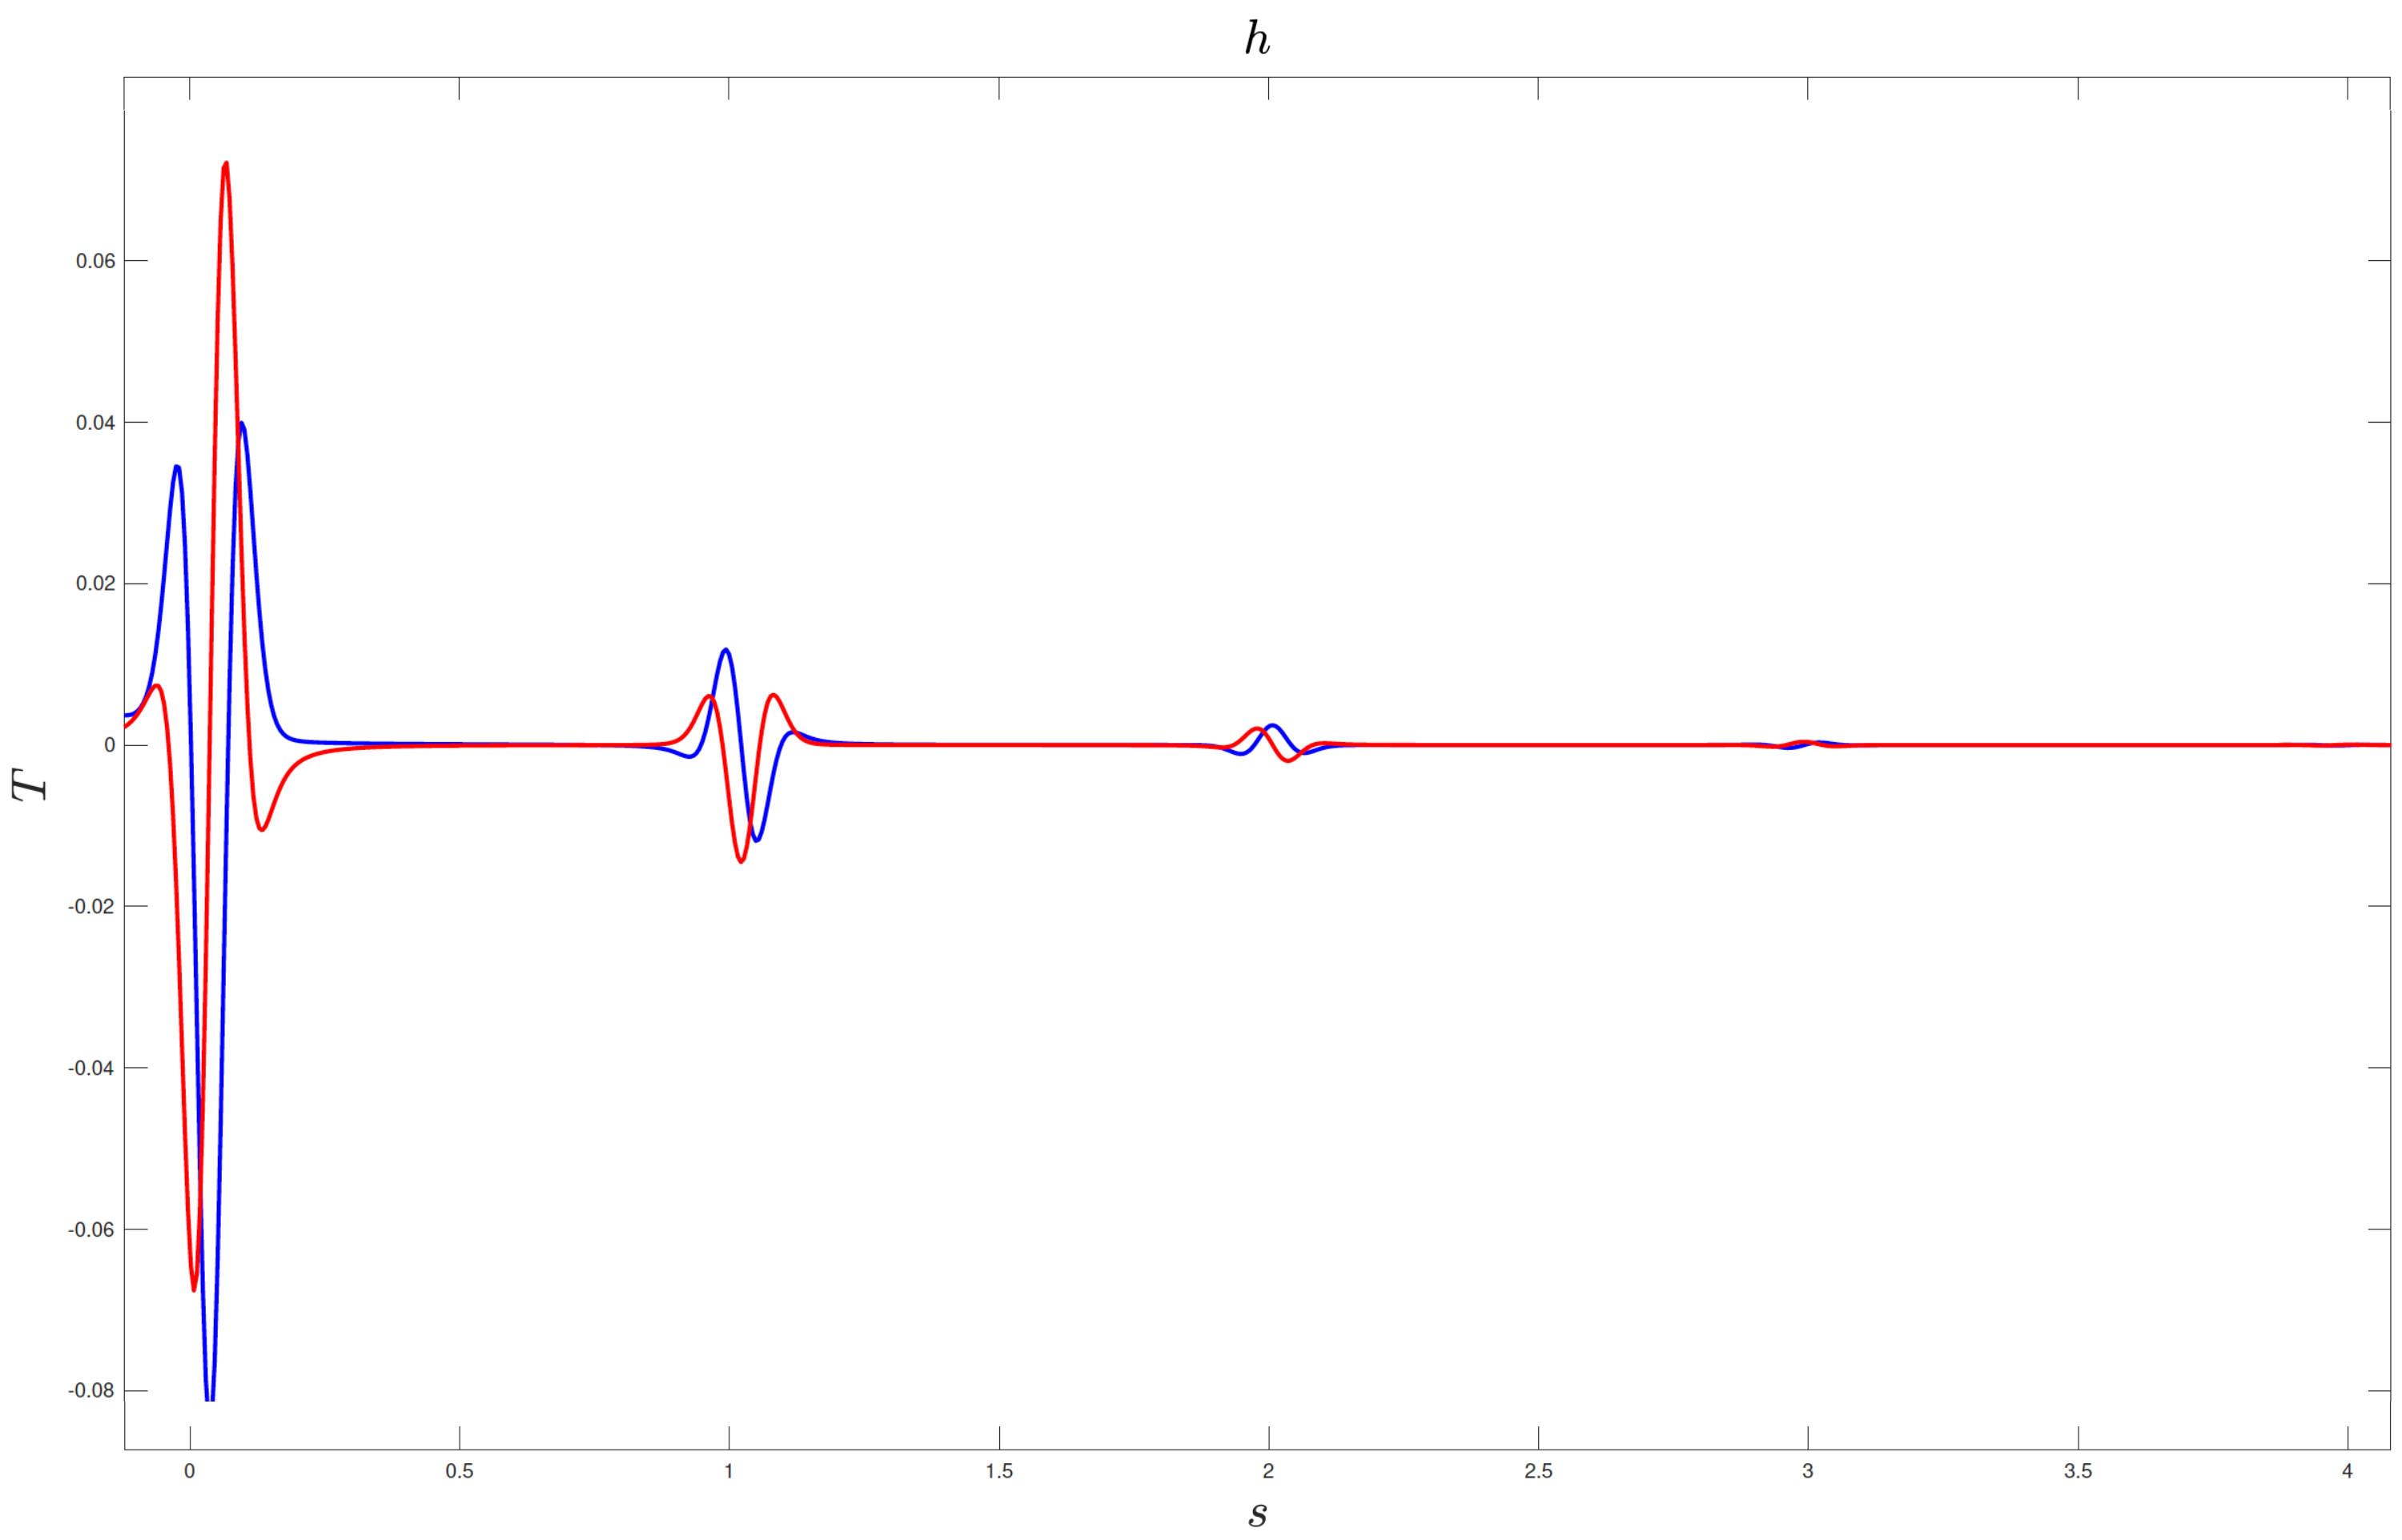
\includegraphics[scale=.94]{four_partially_1D_high_ampl_h}\\
\caption{\textit{Podemos observar a chegada da onda direta seguida de uma reflex\~ao e de tr\^es m\'ultiplas da onda eletromagn\'etica.}}
\label{fig.four_partially_1D_electro_hi_ampl}
\end{figure}

At\'e aqui temos simulado propaga\c{c}\~ao com o receptor na superf\'icie, teoricamente junto com a fonte, numa camada de 1000 $m$ de espessura. Mas podemos simular com o receptor em profundidades variadas, e na figura (\ref{fig.four_partially_1D_mech_hi_ampl_250}) vemos uma simula\c{c}\~ao para onda mec\^anica com o receptor a $250\,m$ de profundidade, de onde extra\'imos algumas observa\c{c}\~oes.

\begin{itemize}
\item A chegada da onda direta (evento 1) n\~ao ocorre mais exatamente no tempo zero (considerando fonte n\~ao causal) como acontece com o receptor na superf\'icie, pois a onda teve que descer por 250 $m$ at\'e que atingisse o receptor.
\item A onda refletida na interface entre as camadas (evento 2) chega com tempo um pouco menor que a reflex\~ao do modelo anterior comparando com a figura (\ref{fig.four_partially_1D_mech_hi_ampl}), por exemplo. De fato, para produzir a reflex\~ao do modelo com receptor na superf\'icie, a onda se propagou por $2000\,m$ ida e volta, e aqui a onda se propagou por $1750\,m$.
\item Existe uma grande diferen\c{c}a de amplitude entre a onda refletida e a onda direta, j\'a que al\'em da perda de energia para o meio durante a propaga\c{c}\~ao houve tamb\'em a perda de energia na interface entre as camadas por conta da onda transmitida para a segunda camada.
\item A onda refletida na interface produziu o evento 2, continuou subindo, foi refletida na superf\'icie livre e desceu novamente produzindo o evento 3.
\item Entre os eventos 2 e 3 a onda se propagou por apenas $500\,m$, por isso o evento 3 ocorre rapidamente ap\'os o evento 2.
\item A reflex\~ao na superf\'icie livre \'e praticamente total e n\~ao h\'a onda transmitida para a camada de ar. Assim, h\'a pouca diminui\c{c}\~ao da amplitude do evento 3 em rela\c{c}\~ao ao evento 2, a qual \'e devida somente a perda de energia para o meio durante a propaga\c{c}\~ao.
\item Os eventos 4 e 5 s\~ao m\'ultiplas dos eventos 2 e 3. A grande diminui\c{c}\~ao da amplitude do evento 4 em rela\c{c}\~ao ao evento 3 e a pouca diminui\c{c}\~ao do evento 5 em rela\c{c}\~ao ao 4 ocorrem pelas mesmas raz\~oes dos itens anteriores.
\item Podemos visualizar a ocorr\^encia de mais m\'ultiplas ap\'os o evento 5.
\end{itemize}

\begin{figure}
\centering
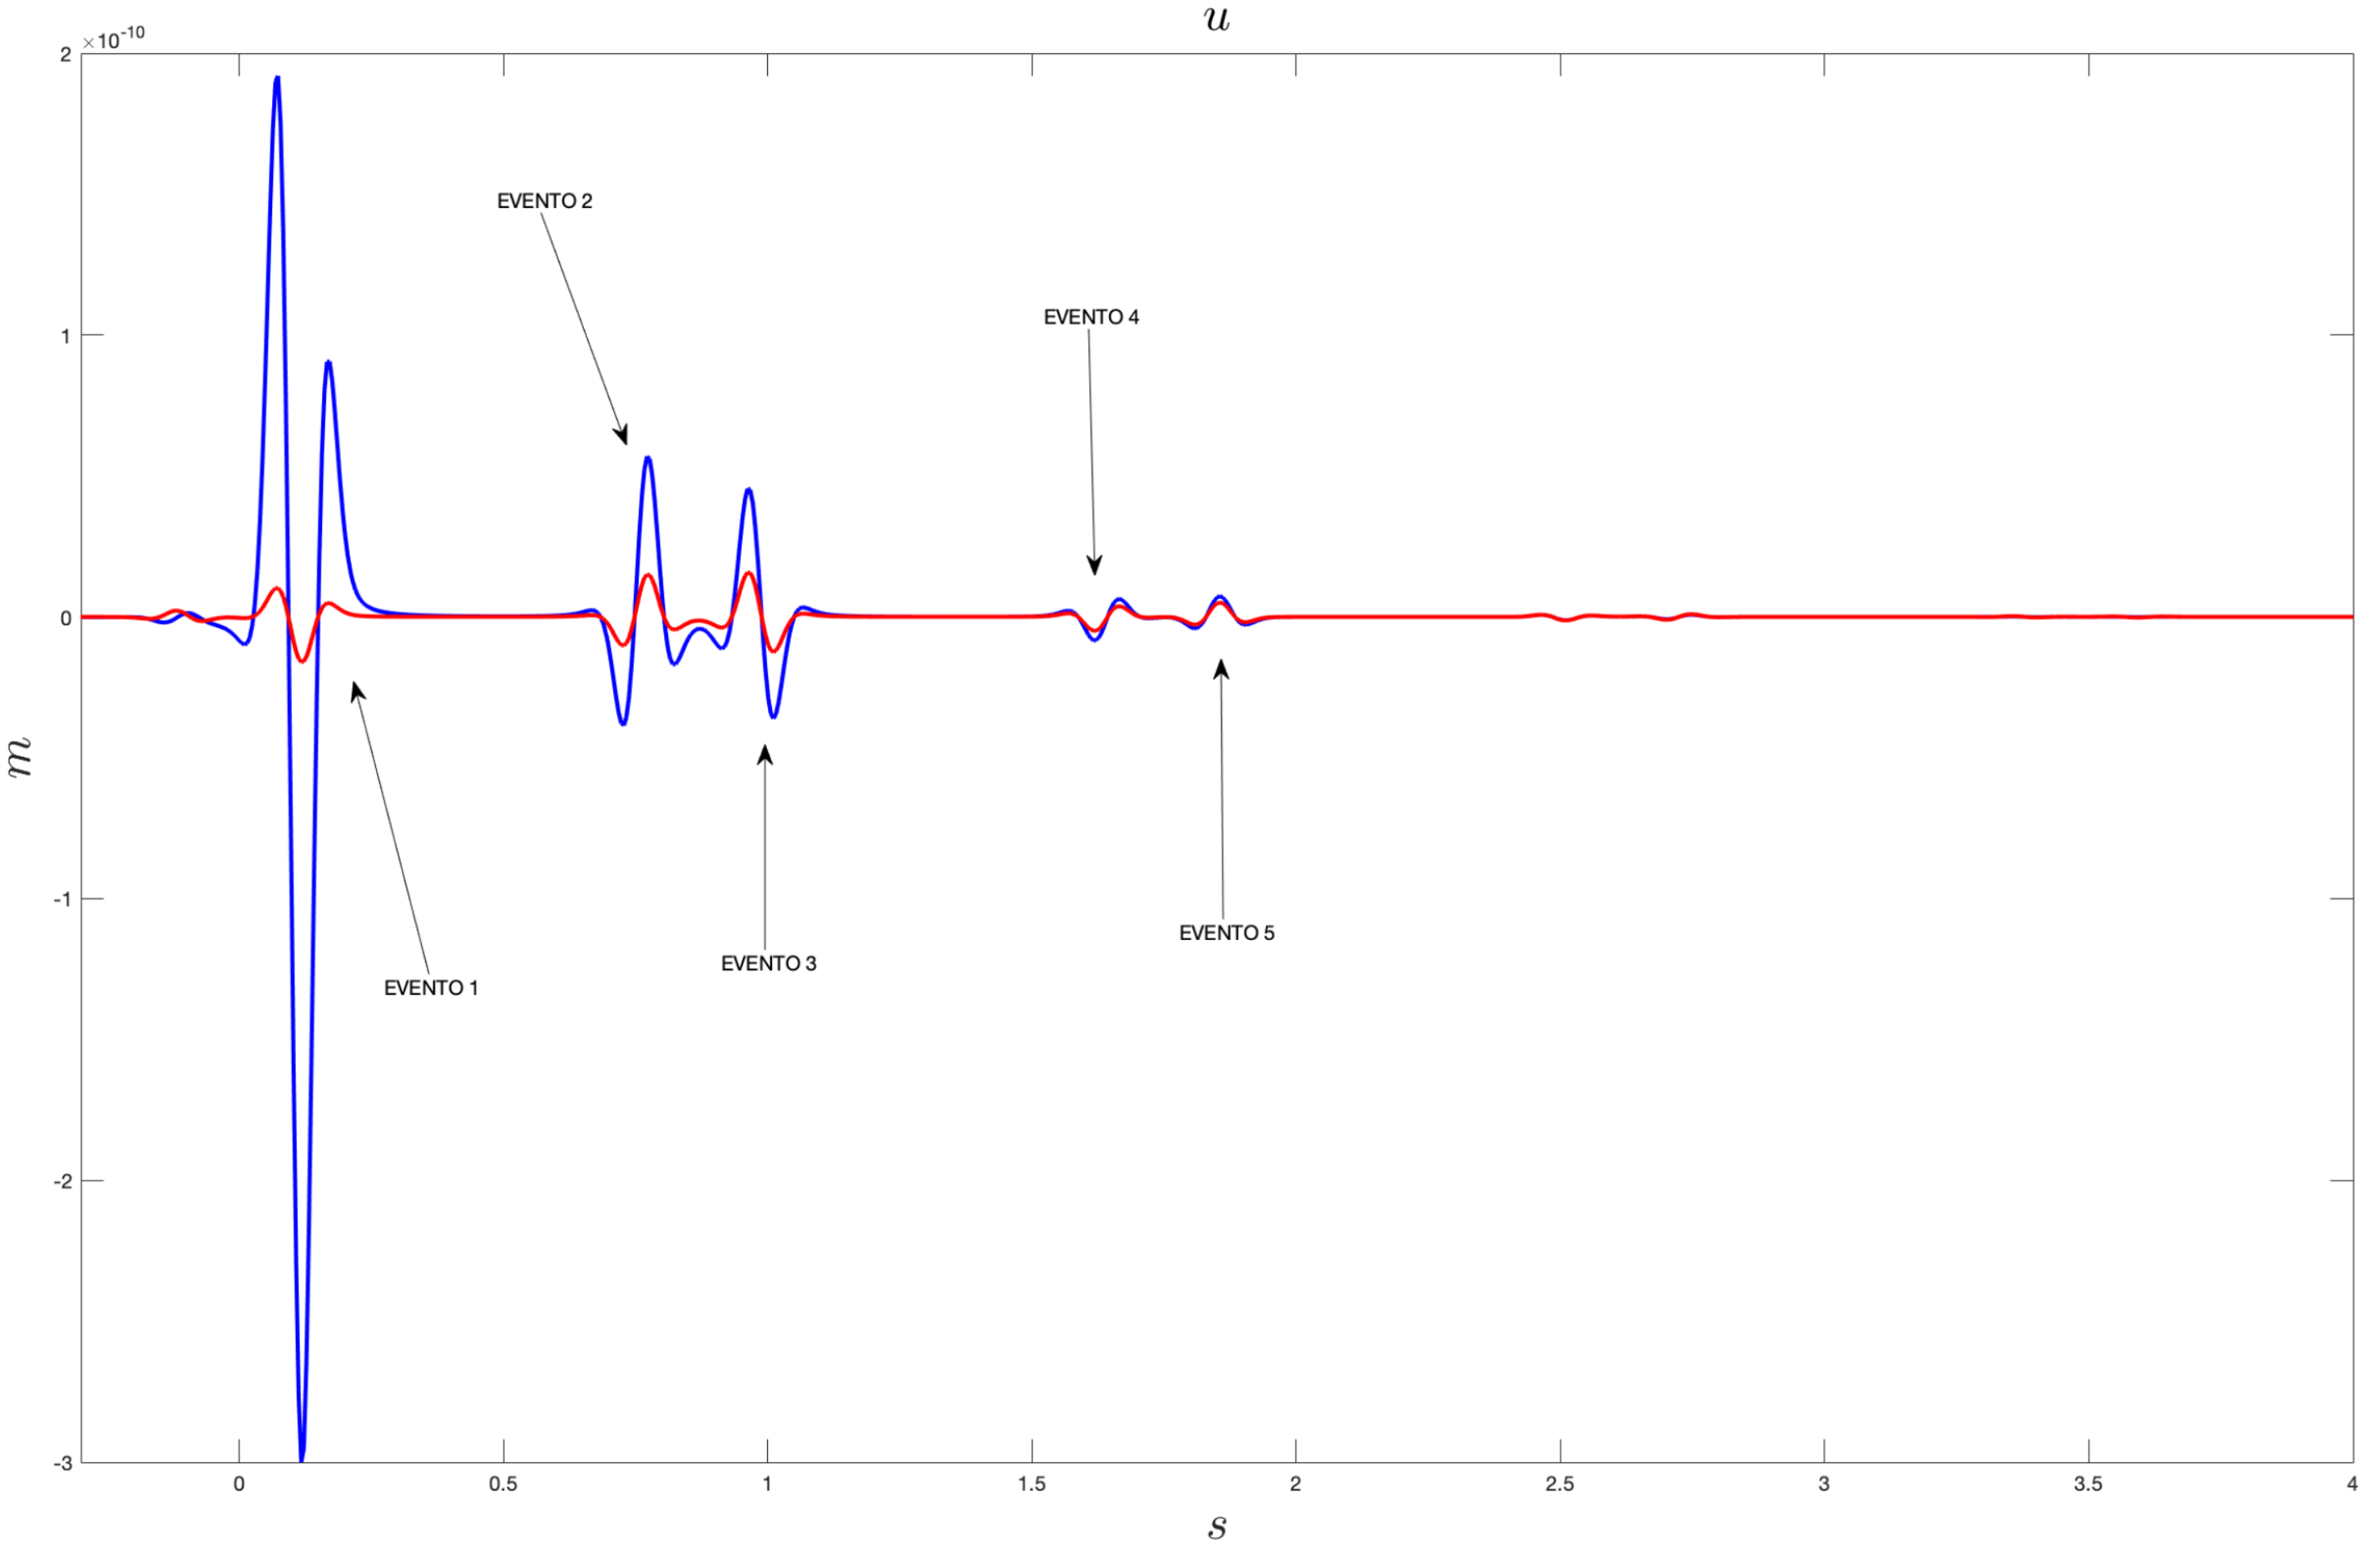
\includegraphics[scale=.775]{four_partially_1D_high_ampl_250_u}\\
\caption{\textit{Camada com 1000 $m$, fonte na superf\'icie e o receptor a 250 $m$ de profundidade.}}
\label{fig.four_partially_1D_mech_hi_ampl_250}
\end{figure}

\begin{figure}
\centering
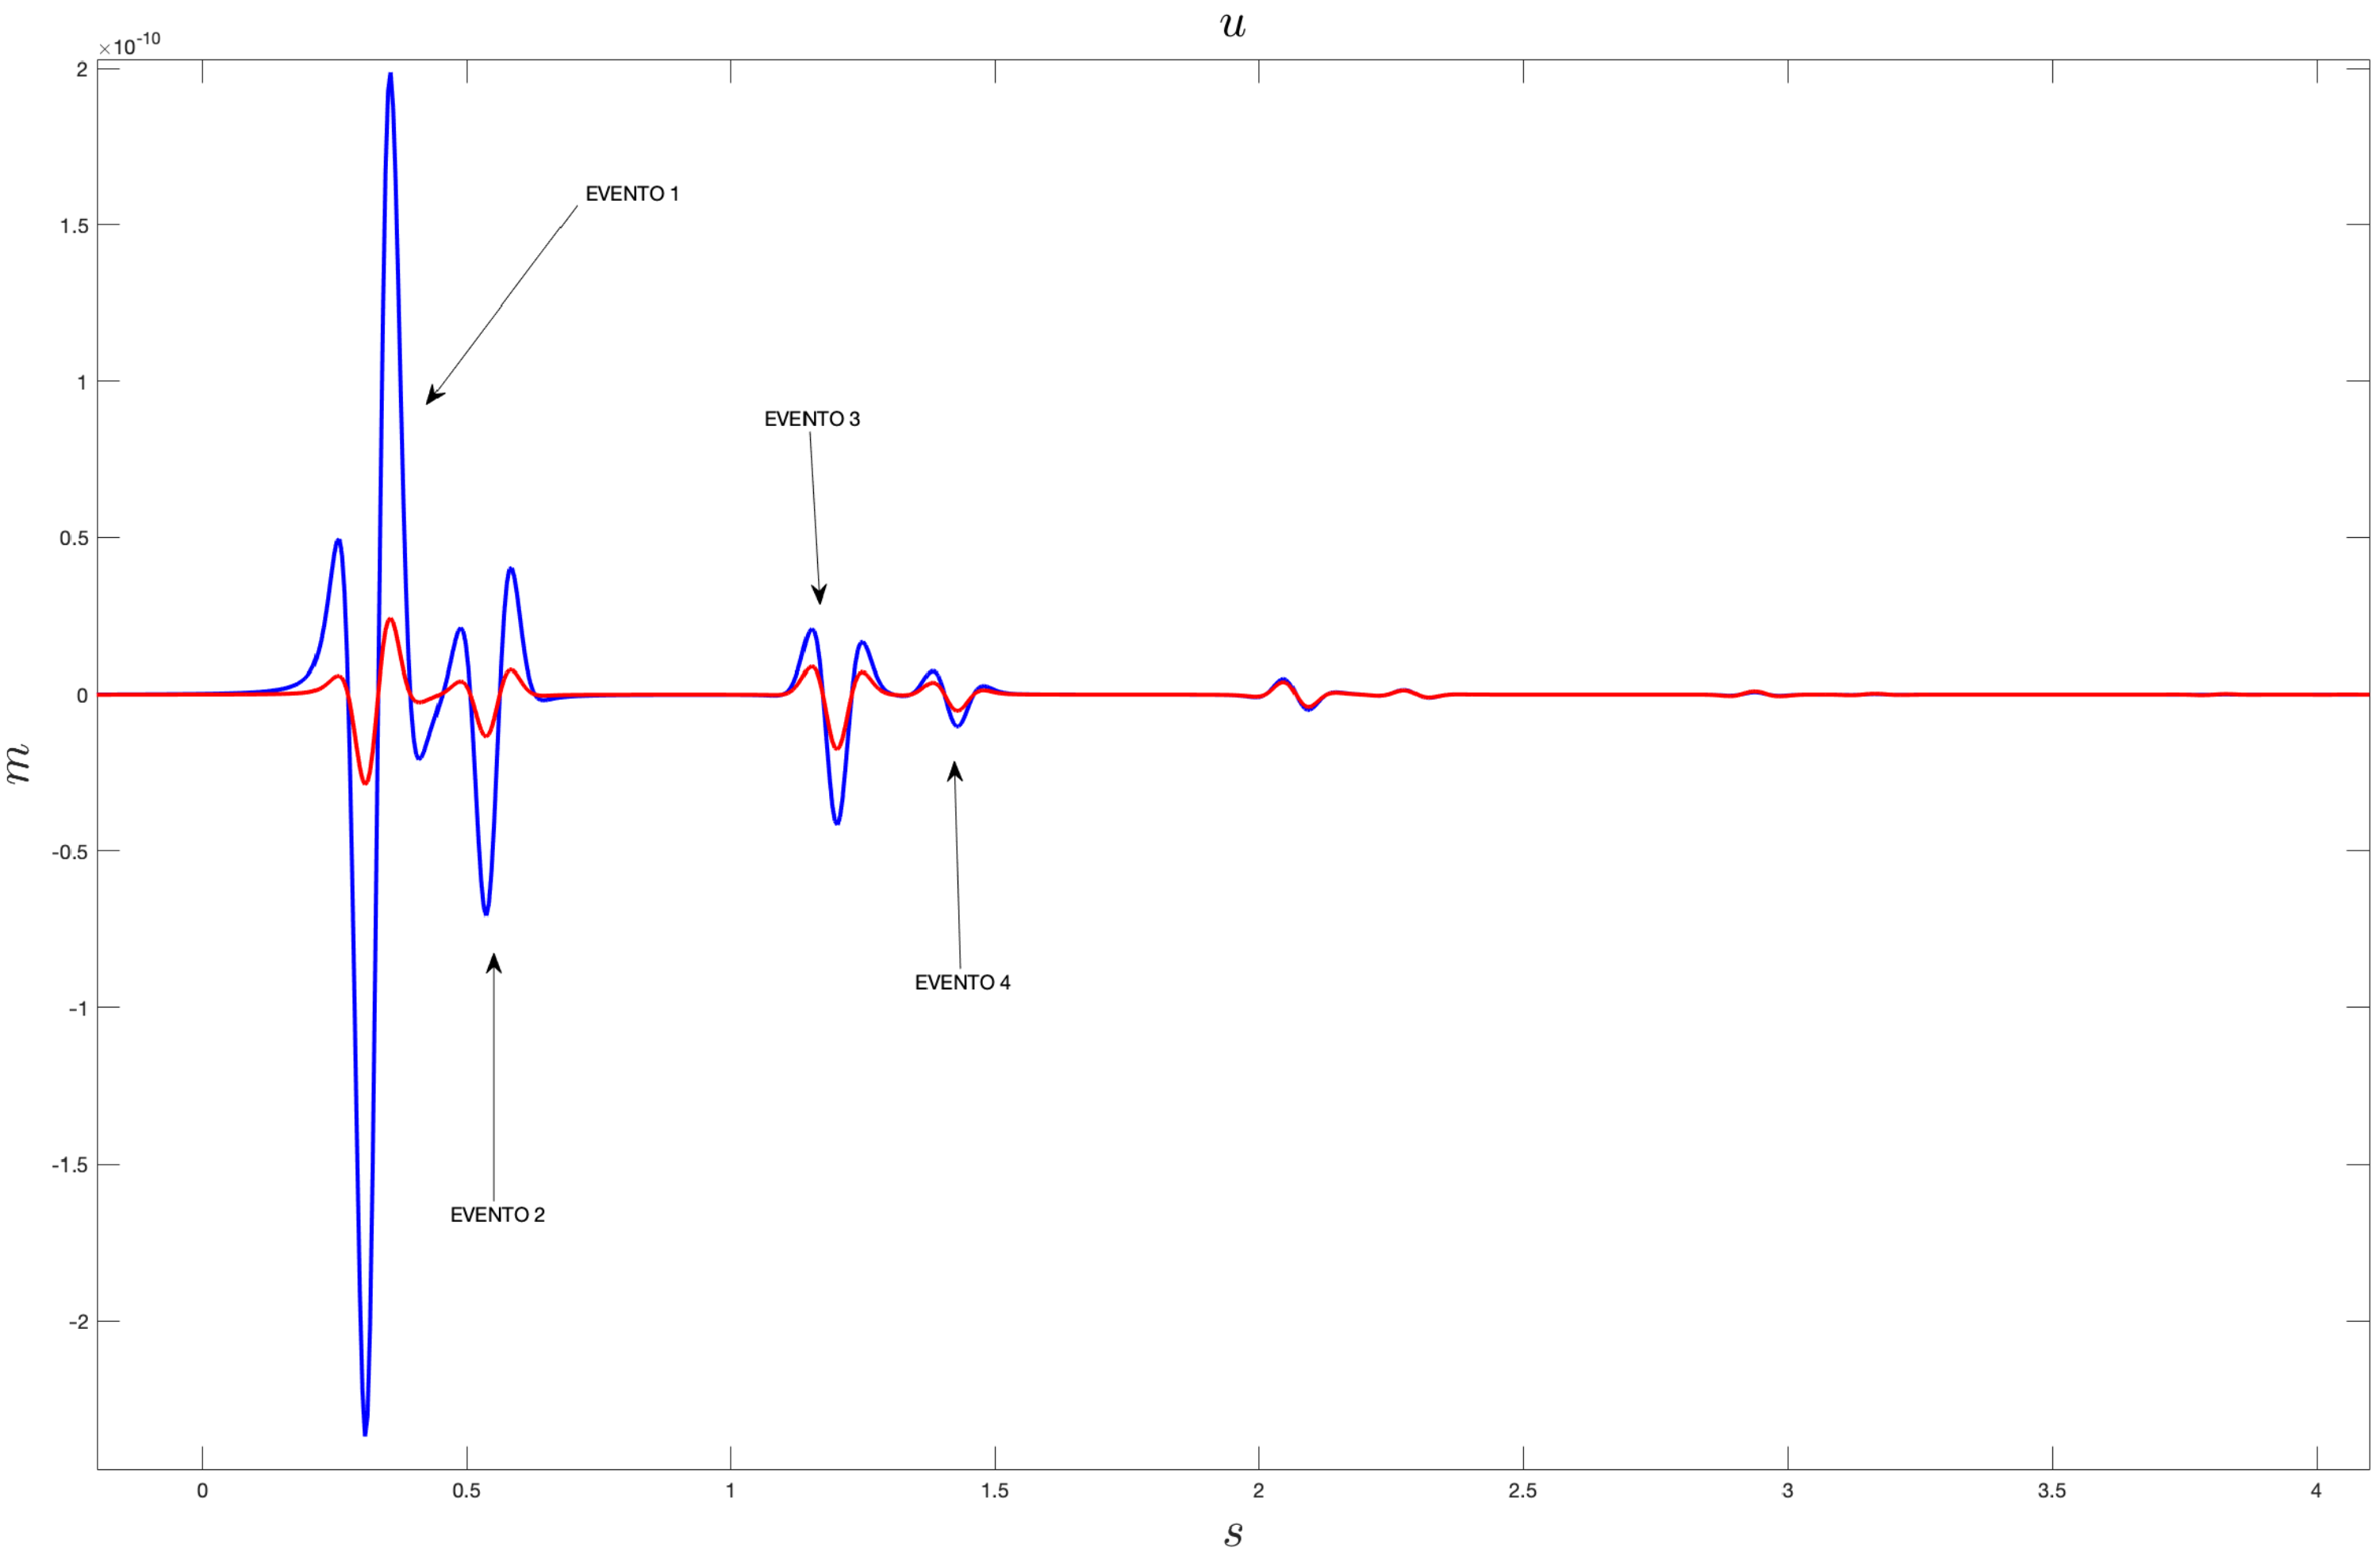
\includegraphics[scale=.87]{four_partially_1D_high_ampl_750_u}\\
\caption{\textit{Camada com 1000 $m$, fonte na superf\'icie e o receptor a 750 $m$ de profundidade.}}
\label{fig.four_partially_1D_mech_hi_ampl_750}
\end{figure}

Na figura (\ref{fig.four_partially_1D_mech_hi_ampl_750}) podemos observar uma simula\c{c}\~ao de propaga\c{c}\~ao de onda mec\^anica numa camada com espessura de 1000 $m$, fonte na superf\'icie e com receptor a 750 $m$ de profundidade, de onde podemos retirar mais algumas observa\c{c}\~oes.

\begin{itemize}
\item O tempo de chegada da onda direta (evento 1) \'e maior que nos dois casos anteriores com receptor na superf\'icie e receptor a $250\,m$ de profundidade. 
\item  Existe pouca diferen\c{c}a de tempo entre a onda direta e a onda refletida na interface (evento 2), pois o receptor se encontra pr\'oximo \`a interface e entre esses eventos a onda se propagou por apenas $500\,m$.
\item A onda refletida na interface (evento 2) atinge o receptor com amplitude bem menor que da onda direta (evento 1), pois h\'a perda de energia da onda transmitida para a segunda camada.
\item O tempo, desde o acionamento da fonte, com que a onda refletida na interface (evento 2) atinge o receptor \'e menor que nos dois casos anteriores (figuras (\ref{fig.four_partially_1D_mech_hi_ampl}) e (\ref{fig.four_partially_1D_mech_hi_ampl_250})), pois aqui essa onda se propagou por uma dist\^ancia menor, $1250\,m$.
\item Ap\'os produzir o evento 2, a onda refletida na interface continua subindo, \'e refletida na superf\'icie livre e desce novamente para produzir o evento 3, completando um ciclo. Ou seja, o evento 3 \'e uma m\'ultipla do evento 1.
\item A diminui\c{c}\~ao de amplitude do evento 3 em rela\c{c}\~ao ao evento 2 n\~ao \'e muito grande, pois a onda sofre reflex\~ao total na superf\'icie livre, e a diminui\c{c}\~ao de amplitude detectada deve-se basicamente a perda de energia para o meio durante a propaga\c{c}\~ao.
\item O evento 4 (m\'ultipla do evento 2) \'e a segunda reflex\~ao na interface e atinge o receptor, comparando com o evento 3, num tempo curto e com amplitude bastante reduzida por conta da energia transmitida para segunda camada.
\item Podemos visualizar mais m\'ultiplas ap\'os o evento 4.
\end{itemize}

\section{Ondas em Meio Estratificado se Propagando em tr\^es Dimens\~oes}
Nesse modelo onde consideramos a propaga\c{c}\~ao em tr\^es dimens\~oes podemos estudar tamb\'em o comportamento da onda transversal, ou onda $S$. A geometria estratigr\'afica \'e composta por tr\^es camadas: a camada 1 com $1000\,m$ de profundidade e superf\'icie livre de contato com o ar, a camada 2 com $500\,m$ de profundidade, interface superior de contato com a camada 1 e interface inferiror de contato com a camada 3, onde a camada 3 possui profundidade infinita. Analisamos somente as ondas que se propagam nas camadas 1 e 2, e as caracter\'isticas das tr\^es camadas est\~ao na tabela (\ref{tab.dados_propagacao}). Assim, nas figuras (\ref{fig.v3}) e (\ref{fig.v3_750}) observamos tra\c{c}os s\'ismicos com v\'arias amplitudes que representam as chegadas de ondas $P$ ou $S$ refletidas na primeira ou segunda interfaces, bem como suas m\'ultiplas.

No cap\'itulo (\ref{sec.disp_aten_mag_elastico}), constatamos que a influ\^encia de campos eletromagn\'eticos em campos mec\^anicos \'e desprez\'ivel em rela\c{c}\~ao a an\'alise de dispers\~ao e atenua\c{c}\~ao, em simula\c{c}\~oes com v\'arios modelos. De acordo com as subse\c{c}\~oes (\ref{sec.prop_homo_1D}) e (\ref{sec.prop_strat_1D}), constatamos ainda que a influ\^encia de campos eletromagn\'eticos em campos mec\^anicos tamb\'em \'e desprez\'ivel em modelos de propaga\c{c}\~ao em uma dimens\~ao tanto homog\^eneos como estratificados. Essas duas constata\c{c}\~oes sugerem que essa influ\^encia continue sendo desprez\'ivel para modelos de propaga\c{c}\~ao em tr\^es dimens\~oes, e isso se constitui numa nova hip\'otese simplificadora para nosso problema, j\'a que n\~ao \'e poss\'ivel ajustar nosso modelo ao formato preconizado por \cite{Ursin-1983}, nem mesmo com a adapta\c{c}\~ao do algoritmo usada nos casos anteriores. Assim, estudamos o caso de propaga\c{c}\~ao em tr\^es dimens\~oes usando apenas o modelo para sistemas parcialmente acoplados, onde analisamos o comportamento somente de campos mec\^anicos para em seguida observar quais influ\^encias esse comportamento mec\^anico provoca em campos eletromagn\'eticos.

\subsection{Modelo para Ondas Mec\^anicas}
Para tratar as ondas mec\^anicas sem influ\^encia dos campos eletromagn\'eticos usamos as equa\c{c}\~oes (\ref{eq.edo_5}) at\'e (\ref{eq.edo_10}), as quais j\'a est\~ao no formato sem aplica\c{c}\~ao da for\c{c}a de \textit{Lorentz}. Para possibilitar a utiliza\c{c}\~ao do m\'etodo matricial dividimos as equa\c{c}\~oes em dois sistemas, onde $v=\dot{\tilde{u}}$ \'e a velocidade de deslocamento do meio.

\begin{empheq}[left=\empheqlbrace]{align}\nonumber
\frac{\partial\,v_3}{\partial\,z}&=-\frac{i\,\omega}{\lambda+2\,G}\,\tilde{\tau}_{33}-\frac{i\,\omega\,\gamma\,\lambda}{\lambda+2\,G}\,v_1\\\nonumber\\\nonumber
\frac{\partial\,\tilde{\tau}_{13}}{\partial\,z}&=-i\,\omega
\left(\rho-\frac{4\,\gamma^2G\,(\lambda+G)}{\lambda+2\,G}\right)\,v_1-\frac{i\,\omega\,\gamma\,\lambda}{\lambda+2\,G}\,\tilde{\tau}_{33}-\tilde{F}_1\\\label{eq.sys_mech_1}\\\nonumber
\frac{\partial\,\tilde{\tau}_{33}}{\partial\,z}&=\frac{\omega\,\rho}{i}\,v_3-i\,\omega\,\gamma\,\tilde{\tau}_{13}-\tilde{F}_3\\\nonumber\\\nonumber
\frac{\partial\,v_1}{\partial\,z}&=-i\,\gamma\,\omega\,v_3-\frac{i\,\omega}{G}\,\tilde{\tau}_{13}
\end{empheq}

\begin{empheq}[left=\empheqlbrace]{align}\nonumber
\frac{\partial\,v_2}{\partial\,z}&=-\frac{i\,\omega}{G}\,\tilde{\tau}_{23}\\\label{eq.sys_mech_2}\\\nonumber
\frac{\partial\,\tilde{\tau}_{23}}{\partial\,z}&=\left[\frac{\omega\,\rho}{i}+\frac{i^2\gamma^2\omega\,G}{i}\right]\,v_2-\tilde{F}_2
\end{empheq}

Come\c{c}ando com o sistema (\ref{eq.sys_mech_1}), temos
\begin{equation*}
M_1^{(\ref{eq.sys_mech_1})}=\begin{pmatrix}
\frac{1}{\lambda+2\,G}&\frac{\gamma\,\lambda}{\lambda+2\,G}\\\\
\frac{\gamma\,\lambda}{\lambda+2\,G}\,&\,\rho-\frac{4\,\gamma^2G\,(\lambda+G)}{\lambda+2\,G}
\end{pmatrix}\,,\quad\quad
M_2^{(\ref{eq.sys_mech_1})}=\begin{pmatrix}
\rho&\gamma\\\\
\gamma&\frac{1}{G}
\end{pmatrix}\quad\text{e}\quad
\mathbf{S}^{(\ref{eq.sys_mech_1})}=\begin{pmatrix}
0\\-F_1\\-F_3\\0
\end{pmatrix},
\end{equation*}
e os autovetores s\~ao
\begin{equation*}
\mathbf{a}_1^{(\ref{eq.sys_mech_1})}=
\sqrt{\frac{q_1}{ \rho+2\,\gamma\,a_1+\frac{a_1^2}{G}}}
\begin{pmatrix}
1\\
a_1
\end{pmatrix}\quad\text{e}\quad
\mathbf{a}_2^{(\ref{eq.sys_mech_1})}=
\sqrt{\frac{q_2}{a_2^2\rho+2\,\gamma\,a_2+\frac{1}{G}}}
\begin{pmatrix}
a_2\\
1
\end{pmatrix}
\end{equation*}\\
\begin{equation*}
\mathbf{b}_1^{(\ref{eq.sys_mech_1})}=\frac{1}{q_1}M_2^{(\ref{eq.sys_mech_1})}\mathbf{a}_1^{(\ref{eq.sys_mech_1})}
\quad\text{e}\quad
\mathbf{b}_2^{(\ref{eq.sys_mech_1})}=\frac{1}{q_2}M_2^{(\ref{eq.sys_mech_1})}\mathbf{a}_2^{(\ref{eq.sys_mech_1})},
\end{equation*}
onde
\begin{equation*}
a_1=\frac{q_1^2- \frac{1}{\lambda+2\,G}  }{\frac{\gamma\,\lambda}{\lambda+2\,G}}\quad\text{e}\quad
a_2=\frac{\frac{\gamma\,\lambda}{\lambda+2\,G}}{q_2^2- \frac{1}{\lambda+2\,G}}.
\end{equation*}
Utilizamos como fonte a aplica\c{c}\~ao de uma for\c{c}a vertical que, no dom\'inio da frequ\^encia angular, \'e dada por
\begin{equation*}
\mathbf{F}=\begin{pmatrix}
0\\
0\\
rck(\omega)
\end{pmatrix}\delta(z-z_s),\quad\text{e como}\quad
\begin{pmatrix}
0\\
-F_1\\
-F_3\\
0
\end{pmatrix}
=-
\begin{pmatrix}
\mathbf{S}_A\\
\mathbf{S}_B
\end{pmatrix}\,\delta(z-z_s),
\end{equation*}
temos que
\begin{equation*}
\mathbf{S}_A^{(\ref{eq.sys_mech_1})}=\begin{pmatrix}
0\\
0
\end{pmatrix}\quad\text{e}\quad
\mathbf{S}_B^{(\ref{eq.sys_mech_1})}=\begin{pmatrix}
rck(\omega)\\
0
\end{pmatrix}.
\end{equation*}
Estabelecemos as condi\c{c}\~oes de contorno usando as encontradas em \cite{pride_94}, que s\~ao $\tau_{13}=\tau_{33}=0$, e a solu\c{c}\~ao imediatamente abaixo da superf\'icie \'e
\begin{equation*}
\Phi(0^+)^{(\ref{eq.sys_mech_1})}=\begin{pmatrix}
v_3\\
0\\
0\\
v_1
\end{pmatrix},\quad\text{e tomando}\quad
\Phi_g^{(\ref{eq.sys_mech_1})}=\begin{pmatrix}
v_3\\
v_1
\end{pmatrix},
\end{equation*}
temos que
\begin{equation*}
G_A^{(\ref{eq.sys_mech_1})}=\begin{pmatrix}
1&0\\
0&0
\end{pmatrix}\quad\text{e}\quad
G_B^{(\ref{eq.sys_mech_1})}=\begin{pmatrix}
0&0\\
0&1
\end{pmatrix}.
\end{equation*}

Para o sistema (\ref{eq.sys_mech_2}), temos 
\begin{equation*}
M_1^{(\ref{eq.sys_mech_2})}=\begin{pmatrix}
\frac{1}{G}
\end{pmatrix}\,,\quad\quad
M_2^{(\ref{eq.sys_mech_2})}=\begin{pmatrix}
\rho-G\,\gamma^2
\end{pmatrix}\quad\text{e}\quad
\mathbf{S}^{(\ref{eq.sys_mech_2})}=\begin{pmatrix}
0\\-F_2
\end{pmatrix},
\end{equation*}
e os autovetores s\~ao
\begin{equation*}
\mathbf{a}^{(\ref{eq.sys_mech_2})}=
\sqrt{\frac{q}{\rho-G\,\gamma^2}}
\quad\text{e}\quad
\mathbf{b}^{(\ref{eq.sys_mech_2})}=
\sqrt{\frac{\rho-G\,\gamma^2}{q}}.
\end{equation*}
Incluindo a fonte no m\'etodo matricial, temos
\begin{equation*}
\begin{pmatrix}
0\\
-F_2
\end{pmatrix}
=-
\begin{pmatrix}
S_A\\
S_B
\end{pmatrix}\,\delta(z-z_s)\quad\text{e, portanto,}\quad
\mathbf{S}_A^{(\ref{eq.sys_mech_2})}=\mathbf{S}_B^{(\ref{eq.sys_mech_2})}=0.
\end{equation*}
Ou seja, o tipo de fonte que estamos usando n\~ao produz onda para o sistema (\ref{eq.sys_mech_2}), pois esse sistema \'e respons\'avel por ondas $SH$, como podemos ver em \cite{pride_94}.

Na figura (\ref{fig.v3}), observamos o tra\c{c}o s\'ismico de uma onda mec\^anica obtido em simula\c{c}\~ao com o sistema (\ref{eq.sys_mech_1}), usando fonte e receptor na mesma posi\c{c}\~ao na superf\'icie.
\begin{figure}
\centering
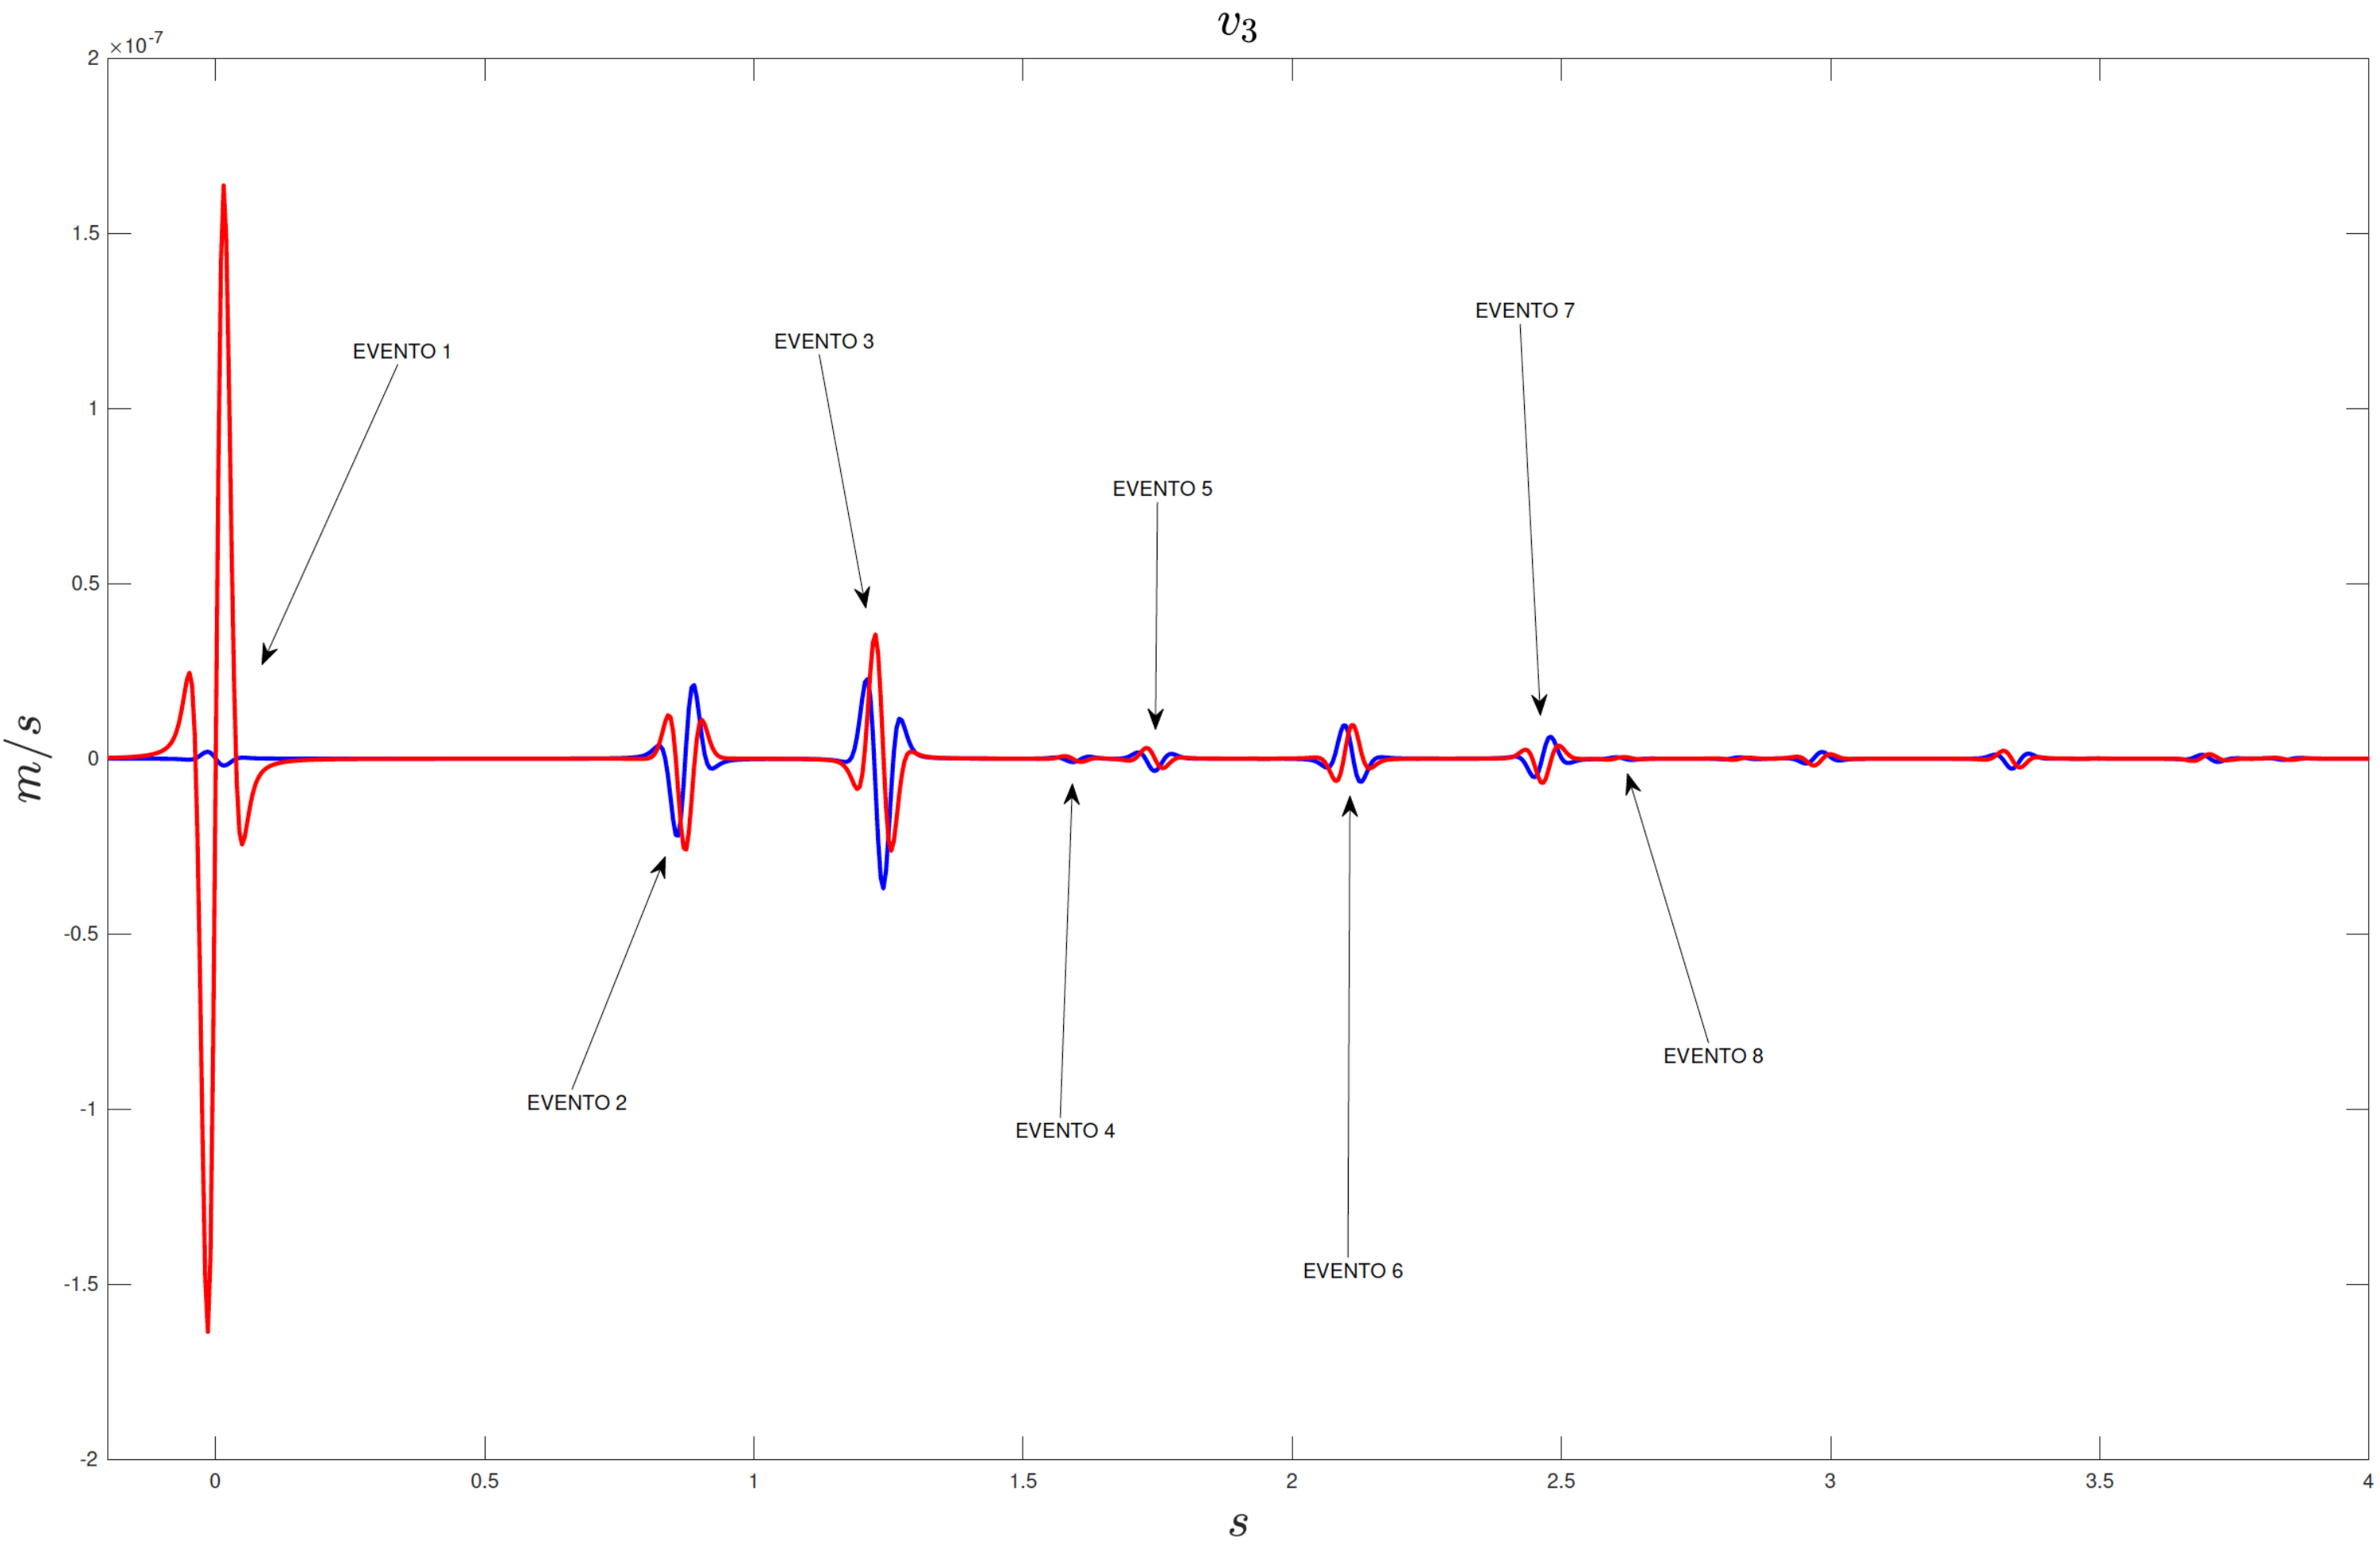
\includegraphics[scale=.775]{v3}\\
\caption{\textit{Modelo tridimensional, primeira camada com 1000 $m$, segunda camada com 500 $m$, fonte e o receptor na superf\'icie.}}
\label{fig.v3}
\end{figure}
Vamos listar algumas observa\c{c}\~oes sobre essa propaga\c{c}\~ao:
\begin{itemize}
\item A ocorr\^encia do evento 1 no tempo zero mostra que este representa a onda direta, j\'a que receptor e fonte est\~ao juntos. Note que a amplitude da onda direta est\'a relativamente pequena.
\item O evento 2 ocorre no tempo necess\'ario para a onda $P$ realizar a propaga\c{c}\~ao de ida e volta entre a superf\'icie e a primeira interface, mostrando que este evento representa a reflex\~ao na primeira interface. 
\item O evento 3 ocorre no tempo necess\'ario para que a onda $S$ se propague ida e volta da superf\'icie at\'e a primeira interface, portanto \'e a reflex\~ao da onda $S$ na primeira interface. De fato, a amplitude do evento 3 \'e maior que do evento 2, comportamento comum entre ondas $P$ e $S$ como podemos observar em v\'arios sism\'ografos.
\item O tempo de chegada do evento 4 coincide com o tempo necess\'ario para onda longitudinal ser refletida na segunda interface.
\item O evento 5 tem o dobro do tempo de chegada e menor amplitude que o evento 2, mostrando que o mesmo \'e uma m\'ultipla da onda longitudinal refletida na primeira interface.
\item O evento 4 \'e de uma onda $P$ que viajou por $3000\,m$ e o evento 5 de uma onda $P$ que viajou por $4000\,m$, mas o evento 4 tem amplitude menor que do evento 5. Isso acontece porque o evento 4 passou por tr\^es processos (duas transmiss\~oes e uma reflex\~ao) de perda de energia em interfaces, enquanto o evento 5 passou por dois processos. 
\item O evento 6 tem o tempo de chegada compat\'ivel com o tempo necess\'ario para reflex\~ao de uma onda transversal na segunda interface. Note que o evento 6 tem amplitude e tempo de chegada maiores que do evento 4.
\item O evento 7 tem o dobro do tempo de chegada do evento 3, ou seja, \'e uma m\'ultipla da onda transversal refletida na primeira interface.
\item O evento 8 tem tr\^es vezes o tempo de chegada do evento 2, ou seja, \'e a segunda m\'ultipla da reflex\~ao da onda $P$ na primeira interface.
\end{itemize}

\begin{figure}
\centering
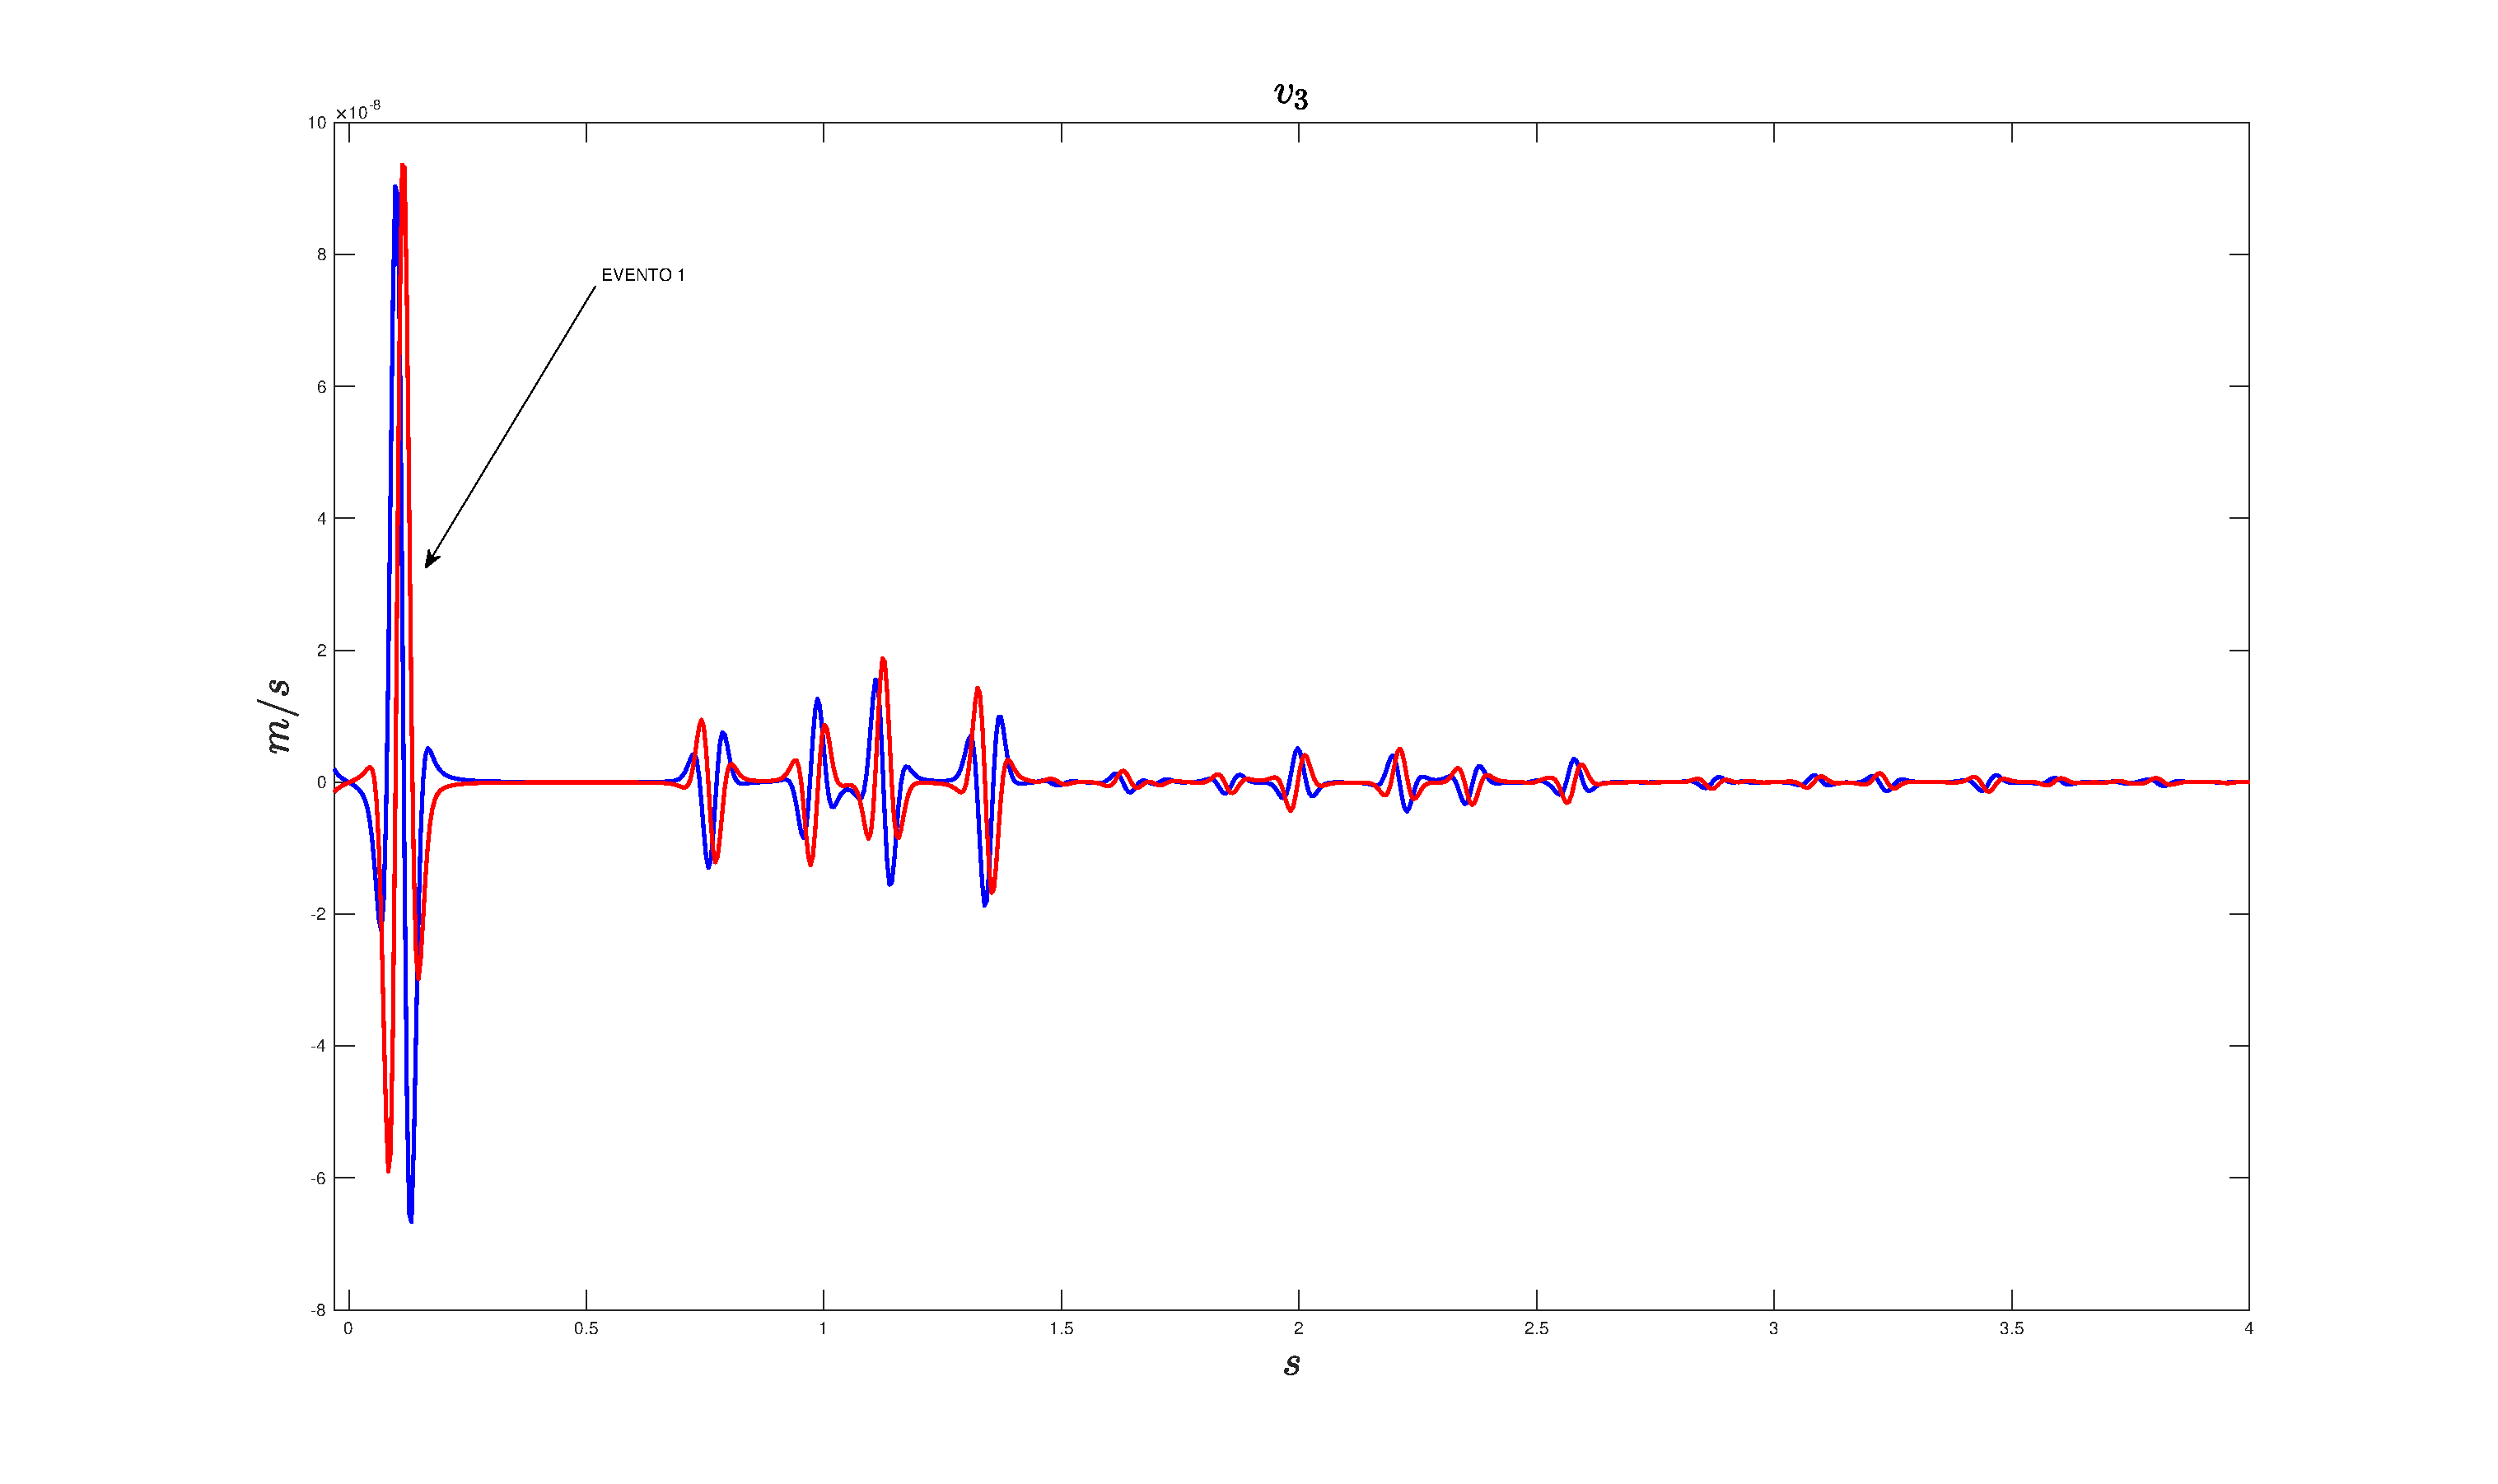
\includegraphics[scale=.678]{v3_250}\\
\caption{\textit{Modelo tridimensional, primeira camada com 1000 $m$, segunda camada com 500 $m$, fonte na superf\'icie e o receptor a 250 $m$ de profundidade verticalmente abaixo da fonte.}}
\label{fig.v3_250}
\end{figure}

Podemos observar, na figura (\ref{fig.v3}) que a amplitude da onda direta (evento 1) n\~ao est\'a satisfat\'oria como em casos anteriores. Nessa abordagem para o caso tridimensional temos uma quantidade maior de coeficientes e o algebrismo se torna menos trabalhoso se usarmos a velocidade de deslocamento do meio do que o pr\'oprio deslocamento do meio, pois economizamos a manipula\c{c}\~ao de alguns coeficientes. Talvez o algoritmo tenha dificuldade em identificar a velocidade de deslocamento do meio para onda direta quando fonte e receptor est\~ao na mesma posi\c{c}\~ao. Assim, afastamos o receptor da fonte, colocando-o numa profundidade vertical de $250\,m$, similar ao que fizemos anteriormente, e foi poss\'ivel identificar normalmente e chagada da onda direta. Na figura (\ref{fig.v3_250}), temos a chegada da onda direta (evento 1) para o mesmo modelo da figura (\ref{fig.v3}), com a \'unica diferen\c{c}a na dist\^ancia fonte/receptor. Note que o tempo de chegada da onda direta da figura (\ref{fig.v3_250}) coincide com o tempo de chegada da mesma onda na figura (\ref{fig.four_partially_1D_mech_hi_ampl_250}), pois em ambos os casos temos a mesma dist\^ancia fonte/receptor.\\













































%\chapter{Conclusões e Trabalhos Futuros}

Muitas pesquisas v\^em sendo realizadas no sentido de efetuar simula\c{c}\~oes num\'erico-computacionais que possam descrever diversos fen\^omenos f\'isicos relacionados \`a prospec\c{c}\~ao de petr\'oleo ou outro bem mineral, assim como fen\^omenos f\'isicos relacionados a terremotos ou que se aplicam a outros objetos de estudo. Essas simula\c{c}\~oes s\~ao ainda confrontadas com experimentos de campo na busca por consist\^encia entre essas duas faces do desenvolvimento de uma teoria. Numa oportunidade futura vamos desenvolver de forma anal\'itico-matem\'atica as EDP's da magneto-elasticidade,  e em seguida criar um algoritmo computacional capaz de efetuar simula\c{c}\~oes que nos auxiliem a estudar o efeito magneto-el\'astico, bem como entender e expandir a teoria geral que trata da intera\c{c}\~ao entre mec\^anica do cont\'inuo e eletromagnetismo em explora\c{c}\~ao de petr\'oleo.

O efeito magneto-el\'astico \'e descrito matematicamente pelo conjunto de EDP's formado pelo sistema de Maxwell e pelo sistema de Lam\`e, os quais s\~ao utilizados no estudo da propaga\c{c}\~ao acoplada de ondas s\'ismicas e eletromagn\'eticas na subsuperf\'icie terrestre. O acoplamento foi caracterizado, primeiramente, pela varia\c{c}\~ao que a for\c{c}a de Lorentz provoca no deslocamento do meio condutivo, simbolizado pela adi\c{c}\~ao da parcela referente \`a esta for\c{c}a na equa\c{c}\~ao do movimento de Cauchy. Segundo, pela a altera\c{c}\~ao eletromagn\'etica gerada pela passagem de uma onda s\'ismica que faz um meio condutivo oscilar no campo geomagn\'etico, simbolizada pela adi\c{c}\~ao desta varia\c{c}\~ao \`a lei de Amp\`ere-Maxwell. Estamos estudando o caso parcialmente acoplado no espaco 3D, mas desejamos analisar tamb\'em o acoplamento total considerando tanto o espa\c{c}o 3D como o espa\c{c}o 1D, esperando que os desenvolvimentos e resultados em cada caso possam se complementar mutuamente.

Algumas hip\'oteses de ordem f\'isica, como o regime quasi-estacion\'ario por exemplo, foram necess\'arias para simplificar o modelo, linearizando as equa\c{c}\~oes e possibilitando o desenvolvimento anal\'itico das mesmas. Sendo assim, buscaremos pelas solu\c{c}\~oes dessas EDP's raciocinando basicamente com duas alternativas. Uma delas \'e trasnsformar as EDP's em EDO's utilizando ferramentas como as transformadas laterais de Fourier, transformadas de Hankel e mudan\c{c}as de eixos coordenados, escrevendo as equa\c{c}\~oes num formato onde \'e poss\'ivel aplicar um metodo matricial espec\'ifico para estudo de propaga\c{c}\~ao de ondas em meios estratigr\'aficos. Outra alternativa \'e reescrever as equa\c{c}\~oes em coordenadas cil\'indricas e fazer uso da hip\'otese de isotropia do meio de propaga\c{c}\~ao para reduzir as dimens\~oes do problema e obter as EDO's nas quais o m\'etodo matricial \'e aplicado.
\\
Neste trabalho apresentamos um tratamento matem\'atico das EDP's do efeito magneto-el\'astico encontrado em \cite{pinho_2018} , no sentido de propiciar a contru\c{c}\~ao de um algoritmo num\'erico est\'avel que possa descrever a propaga\c{c}\~ao acoplada de ondas el\'asticas e eletromagn\'eticas. Nesse tratamento foi fundamental a aplica\c{c}\~ao de conhecimentos da F\'isica-Matem\'atica, Geof\'isica e, em particular, um metodo matricial que facilita a an\'alise de propaga\c{c}\~ao de ondas em meios estratificados.

Vimos na subse\c{c}\~ao \ref{sec.matricial_poroelast} a possibilidade de an\'alise de dispers\~ao e de atenua\c{c}\~ao de ondas para casos diversos, onde tal an\'alise auxilia na verifica\c{c}\~ao e constru\c{c}\~ao de um c\'odigo computacional efetivo para descrever a propaga\c{c}\~ao dessas ondas. Numa oportuinidade futura, queremos aplicar a an\'alise de atenua\c{c}\~ao e dispers\~ao nesse sistema de EDP's do efeito magneto-el\'astico com a finalidade de ajudar a estudar o comportamento da propaga\c{c}\~ao.

Numa determinada abordagem, a an\'alise de casos mais simples auxilia no estudo de casos mais sofisticados. Por tanto, no intuito ainda de otimizar o estudo da propaga\c{c}\~ao das ondas, faremos o tratamento matem\'atico das EDP's de magneto-elasticidade para o caso unidimensional, considerando a propaga\c{c}\~ao em fun\c{c}\~ao do tempo e em fun\c{c}\~ao da profundidade. Neste caso podemos utilizar o m\'etodo matricial e a an\'alise de atenua\c{c}\~ao e dispers\~ao das ondas, e economizamos a utiliza\c{c}\~ao de transformadas e mudan\c{c}a de eixos coordenados.

O formato final das EDO's dado no cap\'itulo \ref{sec.trans_edp_2_edo} apresentou algumas vari\'aveis incluidas como fonte, diferentemente do que \'e preconizado por Ursin, onde todas a vari\'aveis devem estar inseridas no vetor $\mathbf{\Phi}$. Assim, analisaremos a possibilidade da aplica\c{c}\~ao de fun\c{c}\~oes de Green juntamente com o m\'etodo matricial para contornar esse problema. \'E poss\'ivel que essa abordagem traga desafios computacionais consider\'aveis e da\'i estudaremos tamb\'em outras alternativas. Uma delas \'e considerar o efeito magento-el\'astico para o caso totalmente acoplado e verificar se o novo formato das equa\c{c}\~oes permite a exclus\~ao de vari\'avies dadas como fonte. Outra possibilidade \'e escrever as equa\c{c}\~oes em coordenadas cil\'indricas, considerar as propriedades de isotropia das camadas e substituir as coordenadas horizontais somente pelo raio.

A implementa\c{c}\~ao do algoritmo computacional ser\'a realizada em linguagem C++, por conta de algumas caracter\'isticas apresentadas por esta linguagem descritas em \cite{bueno_2015}, como: ser de prop\'osito geral podendo ser utilizada na constru\c{c}\~ao de programas computacionais, aplicativos de sistemas embarcados e em computa\c{c}\~ao cient\'ifica; ser de alto n\'ivel e orientada a objeto, permitindo a propagama\c{c}\~ao simult\^anea realizada por v\'arios programadores trabalhando num mesmo projeto; fortemente tipada o que ajuda na detec\c{c}\~ao de \textit{bugs} e controle e gerenciamento de mem\'oria; ser a mais utilizada em sistemas complexos e grandes no uso de programa\c{c}\~ao paralela.

\bibliographystyle{plainnat}
%\bibliography{referencias}

\begin{thebibliography}{25}
\providecommand{\natexlab}[1]{#1}
\providecommand{\url}[1]{\texttt{#1}}
\expandafter\ifx\csname urlstyle\endcsname\relax
  \providecommand{\doi}[1]{doi: #1}\else
  \providecommand{\doi}{doi: \begingroup \urlstyle{rm}\Url}\fi


\bibitem[Cukavac(2008)]{Cukavac_2008}
M.~S. Cukavac.
\newblock Seismomagnetic insvestigations in kopaonik area.
\newblock \emph{MGB}, 2008.

\bibitem[Eringen(1963)]{eringen_1963}
J.W.~Dunkin e A.C.~Eringen.
\newblock On the propagation of waves in an electromagnetic elastic solid.
\newblock \emph{International Journal of Engineering Science}, 1, 1963.


\bibitem[Tromp(1998)]{dahlem}
F.~A.~Dahlem e~J.~Tromp.
\newblock \emph{Theoretical Global Seismology}.
\newblock Princeton University Press, 1998.

\bibitem[Soboleva(1997)]{Mikhailenko_1997}
B.~G.~Mikhailenko e~O.~N.~Soboleva.
\newblock Mathematical modeling of seismomagnetic efects arising in the seismic
  wave motion in the earth's constant magnetic field.
\newblock \emph{Applied Mathematics Lettures}, 10\penalty0 (3):\penalty0
  47--51, 1997.

\bibitem[Pilipenko(1997)]{surkov_97}
V.~V.~Surkov e~V.~A.~Pilipenko.
\newblock Magnetic effects due to earthquakes and underground explosions: a
  review.
\newblock \emph{Annali di Geofisica}, XL\penalty0 (2):\penalty0 227--239, 1997.

\bibitem[Eringen(1962)]{Eringen_1962}
A.~C. Eringen.
\newblock \emph{Nonlinear Theory of Continuous Media}.
\newblock McGraw-Hill New York, 1962.

\bibitem[Griffiths(1999)]{griffiths}
D.~J. Griffiths.
\newblock \emph{Introduction to Electrodynamics}.
\newblock Prentice-Hall, 1999.

\bibitem[Guglielmi(1986a)]{guglielmi_86a}
A.~V. Guglielmi.
\newblock Magnetoelastic waves.
\newblock \emph{Izv. Akad. Nauk SSSR, Fizika Zemli}, 7\penalty0 (112), 1986a.

\bibitem[Guglielmi(1986b)]{guglielmi_86b}
A.~V. Guglielmi.
\newblock Excitation of oscillations of the electromagnetic field by elastic
  waves in the conducting body.
\newblock \emph{Geomagn. Aeron.}, 27\penalty0 (3):\penalty0 467--470, 1986b.

\bibitem[Jackson(1999)]{jackson_classical_1999}
J.~D. Jackson.
\newblock \emph{Classical electrodynamics}.
\newblock Wiley, New York, {NY}, 3rd ed., 1999.


\bibitem[Knopoff(1955)]{Knopoff_1955}
E.~L. Knopoff.
\newblock The interaction between elastic waves motions and magnetic field in
  electrical conductors.
\newblock \emph{J. Geophys. Res.}, 60\penalty0 (4):\penalty0 617--629, 1955.

\bibitem[Yerzhanov(1985)]{yerzhanov_85}
T.~E. Nasynbaev e A. V.~Bushuev L.~S.~Yerzhanov, A. K.~Kurskeev.
\newblock Geomagnetics observations during the massa experiments.
\newblock \emph{Izv. Akad. Nauk SSSR, Fizika Zemli}, 11:\penalty0 80--82, 1985.

\bibitem[Liu(2002)]{liu}
I.~S. Liu.
\newblock \emph{Continuum Mechanics}.
\newblock Spring-Verlag, Berlim-Heidelberg, 2002.

\bibitem[Sadovsky(1980)]{Sadovsky_1980}
M.A. Sadovsky.
\newblock Electro magnetic precursors of earthquakes.
\newblock \emph{Dokl. Acad. Nauka}, 1980.

\bibitem[Slawinski(2007)]{slawinski}
M.~A. Slawinski.
\newblock \emph{Waves And rays in elastic continua}.
\newblock World Scientific Publishing Company, 2 ed, 2007.


\bibitem[Sommerfeld(1952)]{sommerfeld_52}
A.~Sommerfeld.
\newblock Electrodynamics.
\newblock \emph{Academic Press}, 1952.

\bibitem[Stacey(1964)]{stacey_64}
F.~D. Stacey.
\newblock Seismo-magnetic effect.
\newblock \emph{Pure Applied Geophysics}, 58\penalty0 (11):\penalty0 5--23,
  1964.

\bibitem[Surkov(1989a)]{surkov_89a}
V.~V. Surkov.
\newblock Local changes in geomagnetics and geoeletrics fields under rocks
  deformation near the earth surface.
\newblock \emph{Izv. Akad. Nauk SSSR, Fizika Zemli}, 5:\penalty0 91--96, 1989a.

\bibitem[Surkov(1989b)]{surkov_89b}
V.~V. Surkov.
\newblock Distortion of external magnetic field by a longitudinal acoustic
  wave.
\newblock \emph{Magnetic Hydro-Dynamics}, 2:\penalty0 9--12, 1989b.

\bibitem[Anisimov(1985)]{Anisimov_1985}
E.A. Ivanov M.V. Pedanov N.N.Rusakov V.A. Troizhkya e V.E.~Goncharov
  S.V.~Anisimov, M.B.~Gokhberg.
\newblock Short period oscillations of electromagnetic field of the earth after
  explosion.
\newblock \emph{Dokl. Acad. Nauka}, 281\penalty0 (3):\penalty0 556--559, 1985.

\bibitem[Rikitake(1980)]{Rikitake_80}
H.~Tanaka N. Ohshiman Y. Sasai Y. Ishikawa S. Koyama M. Kawamura e K.~Ohchi
  T.~Rikitake, Y.~Honkura.
\newblock Changes in the geomagnetic field associated with earthquakes in the
  izu peninsula, japan.
\newblock \emph{J. Geomag. Geoelectr.}, 32:\penalty0 721--739, 1980.


\bibitem[Azeredo(2013)]{Azeredo_2013}
M.~M. Azeredo.
\newblock \emph{Modelagem Matem\'atica e Computacional da Propaga\c{c}\~ao de
  Ondas S\'ismicas em Meios Poroel\'asticos Estratificados}.
\newblock PhD thesis, Universidade Estadual do Norte Fluminense, 2013.

\bibitem[Baruch(2013)]{baruch_2013}
E.~M. Baruch.
\newblock The classical hankel transform in the kirillov model of discrete
  series.
\newblock \emph{Integral Transforms and Special Functions}, 24, 2013.
%\newblock \doi{10.1080/10652469.2012.691097}.

\bibitem[Bueno(2015)]{bueno_2015}
A.~D. Bueno.
\newblock \emph{Programa\c{c}\~ao Orientada a Objeto com C++}.
\newblock Novatec, 2015.

\bibitem[Butkov(1988)]{butkov_88}
E.~Butkov.
\newblock \emph{F\'isica Matem\'atica}.
\newblock LTC, 1988.

\bibitem[Chew(1995)]{chew}
W.~C. Chew.
\newblock \emph{Waves and Fields in Inhomogeneous Media}.
\newblock IEEE PRESS, 1995.

\bibitem[Dunkin and Eringen(1963)]{eringen_1963}
J.W. Dunkin and A.C. Eringen.
\newblock On the propagation of waves in an electromagnetic elastic solid.
\newblock \emph{International Journal of Engineering Science}, 1, 1963.

\bibitem[Savit(1988)]{dobrin_88}
M.~B.~Dobrin e~C.~H.~Savit.
\newblock \emph{Introduction to Geophysical Prospecting}.
\newblock McGraw-Hill, 1988.

\bibitem[Farlow(1993)]{farlow_93}
S.~J. Farlow.
\newblock \emph{Partial Differential Equations for Scientists and Engineers}.
\newblock Dover, 1993.

\bibitem[Fatianov and Mikhailenko(1989)]{Mikhailenko_89}
A.G. Fatianov and B.G. Mikhailenko.
\newblock Numerically-analytical method for calculation of theoretical
  seismograms in layered-inhomogeneous anelastic media.
\newblock \emph{In Proceedings of the 7 th International Mathematical
  Geophysics Seminar held at the Free University of Berlin}, 1989.

\bibitem[Griffiths(1999)]{griffiths}
D.~J. Griffiths.
\newblock \emph{Introduction to Electrodynamics}.
\newblock Prentice-Hall, 1999.

\bibitem[Lang(1986)]{lang_1986}
S.~Lang.
\newblock \emph{Introduction to Linear Algebra}.
\newblock Springer, 1986.

\bibitem[Lebedev and Cloud(2003)]{lebedev_2003}
L.~P. Lebedev and M.~J. Cloud.
\newblock \emph{Tensor Analysis}.
\newblock World Scientific Publishing, 2003.

\bibitem[Mikhailenko and Soboleva(1997)]{mikhailenko_97}
B.~G. Mikhailenko and O.~N. Soboleva.
\newblock Mathematical modeling of seismomagnetic efects arising in the seismic
  wave motion in the earth's constant magnetic field.
\newblock \emph{Appl. Math. Lett.}, 10\penalty0 (3):\penalty0 47--51, 1997.

\bibitem[Miranda(2016)]{miranda_2016}
M.~R. S.~T. Miranda.
\newblock \emph{M\'etodo Matricial em Modelagem Poroel\'astica: Modelo de
  Biot-JKD}.
\newblock UENF, 2016.

\bibitem[Novacki(1983)]{Novacki_83}
W.~Novacki.
\newblock Electromagnetic efects in solid bodies.
\newblock \emph{In Panstwowe Wydawnictwo Naukowe}, 10, 1983.

\bibitem[Oliveira(2018)]{oliveira_2018}
I.~B. Oliveira.
\newblock \emph{Modelagem de Propaga\c{c}\~ao das Ondas El\'asticas em Meios
  Porosos 1D: Modelo de Biot vs. Biot-JKD}.
\newblock UENF, 2018.

\bibitem[Pinho(2018)]{pinho_2018}
D.~C. Pinho.
\newblock \emph{Fundamentos de Magneto-Elasticidade}.
\newblock UENF, 2018.

\bibitem[Pride(1994)]{pride_94}
S.~Pride.
\newblock Governing equations for the coupled electromagnetics and acustics of
  porous media.
\newblock \emph{Physical Review B}, 1994.

\bibitem[Ursin(1983)]{Ursin-1983}
B.~Ursin.
\newblock Review of elastic and electromagnetic wave propagation in
  horizontally layered media.
\newblock \emph{The Leading Edge}, 48, 08 1983.

\bibitem[Weyl(1919)]{weyl_19}
H.~Weyl.
\newblock Ausbreitung elektromagnetischen wellen ueber einem ebenen leiter.
\newblock \emph{Annalen der Physik}, 1919.

\bibitem[White e Zhou(2006)]{White_Zhou_2006}
B.S. White e M.~Zhou.
\newblock Eletroseismic prospecting in layered media.
\newblock \emph{Society for Industrial and Applied Mathematics}, 67\penalty0
  (1):\penalty0 69--98, 2006.

\bibitem[Blanc(2013)]{Blanc_13}
Blanc, E.
\newblock Time-Domain Numerical Modeling of Poroelastic Waves: The Biot-JKD
Model with Fractional Derivatives.
\newblock \emph{Tese (Doutorado) — AIX-Marseille Université}, December 2013.

\bibitem[Sharma(2008)]{sharma_08}
Sharma, M. D.
\newblock Wave Propagation in Thermoelastic Saturated Porous Medium.
\newblock \emph{J. Earth Syst. Sci.}, 117\penalty0
  (6):\penalty0 951--958, 2008.
  
\bibitem[Abramowitz e Stegun (1964)]{abramovitz_64}
Abramowitz, M. e Stegun, I. A.
\newblock Handbook of Mathematical Functions with Formulas, Graphs, and Mathematical Tables.
\newblock \emph{Dover}, ninth Dover printing, tenth GPO printing, 1964.  
    
  
% LEFT TO BE CITED IN TEXT BODY  
  
  \bibitem[Powell(2011)]{powell_11}
Powell, P. D.
\newblock Calculating Determinants of Block Matrices.
\newblock \emph{arXiv:1112.4379 [math.RA]}, 2011.


\bibitem[Wang(2015)]{wang_15}
Wang, Y.
\newblock Frequencies of the Ricker Wavelet.
\newblock \emph{Geophysics}, 80\penalty0
  (2):\penalty0 A31--A37, 2015.
  
  \bibitem[Chattopadhyay(2011)]{chattopadhyay_11}
A. Chattopadhyay, S. Gupta, A. K. Singh and S. A. Sahu
\newblock G-Type Seismic Wave in Magnetoelastic Monoclinic Layer.
\newblock \emph{Applied Mathematics}, \penalty0
  (2):\penalty0 145--154, 2011.
  
 \bibitem[Jouniaux(2015)]{jouniaux_15}
 L. Jouniaux e F. Zyserman
\newblock Seismo-Electrics, Electro-Seismics, and
Seismo-Magnetics for Earth Sciences.
\newblock \emph{Solid Earth Discuss}, \penalty0
  (7):\penalty0 2563--2662, 2015.
  
  \bibitem[DeBeer(2008)]{beer_08}
 M. De Beer e J. W. Maina
\newblock Some Fundamentals Definitions of the Elastic Parameters for Homogeneous Isotropic Linear Elastic Materials in Pavement Design and Analysis.
\newblock \emph{Proceedings of the Southern African Transport Conference},\penalty0 282--293, 2008.


\end{thebibliography}

\appendix

\chapter{An\'alise de Dispers\~ao e Atenua\c{c}\~ao}\label{sec.app_faraday}
Para o caso citado na subse\c{c}\~ao \ref{sec.faraday}, calculamos a velocidade de fase e atenua\c{c}\~ao de ondas mec\^anicas e eletromagn\'eticas considerando as componentes $u_1$, $u_2$ e $H_3$, escolhendo a dire\c{c}\~ao horizontal de propaga\c{c}\~ao dessas ondas. O gr\'afico \ref{fig.disp_fa_45}  mostra a propaga\c{c}\~ao na dire\c{c}\~ao $45^\circ$ no plano $xy$ e foi confeccionado usando a ferramenta \textit{root} para extrair as ra\'izes de um polin\^omio de grau 6. Observamos o mesmo comportamento da an\'alise feita na subse\c{c}\~ao \ref{sec.faraday}, com a diferen\c{c}a do problema num\'erico gerado pela ferramenta \textit{root}. 

\begin{figure}
\centering
\subfloat{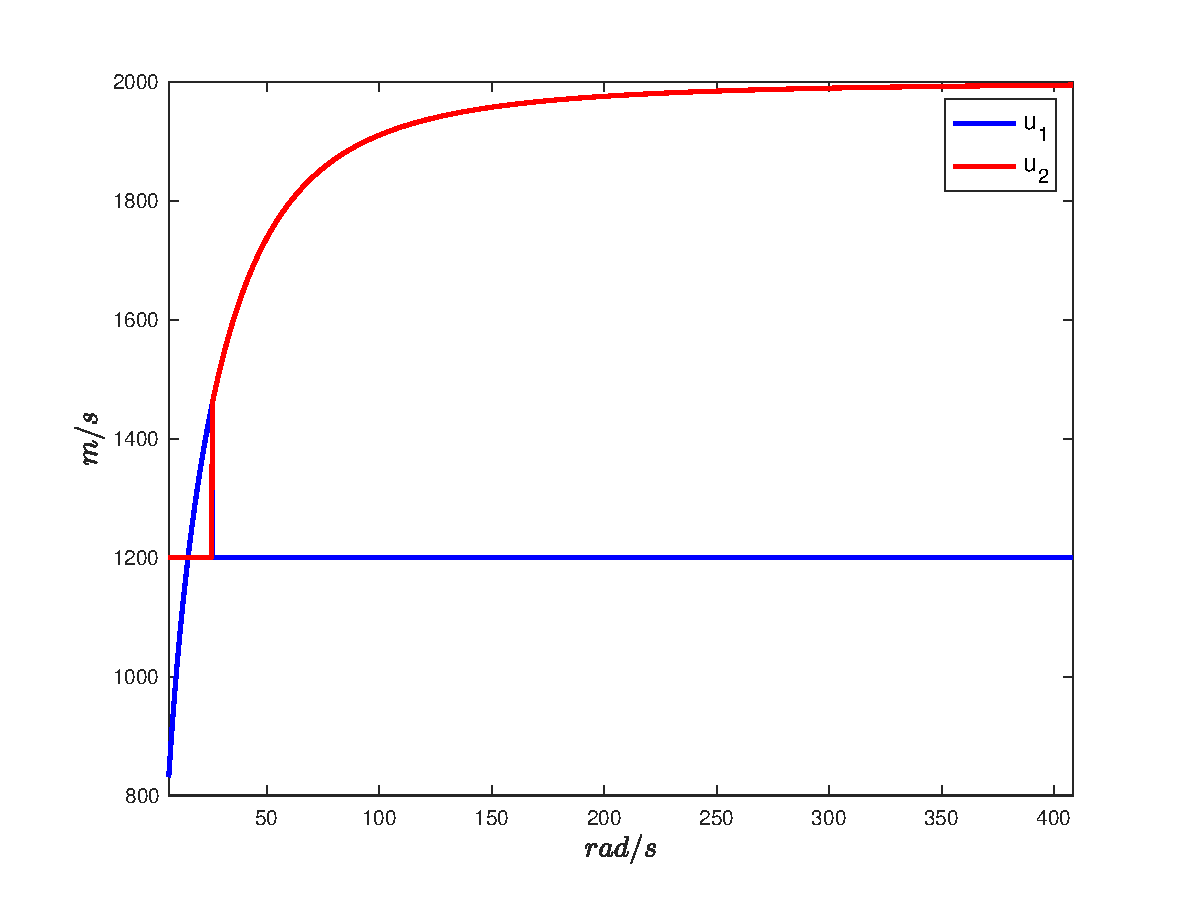
\includegraphics[scale=.425]{app_v_u}}
\subfloat{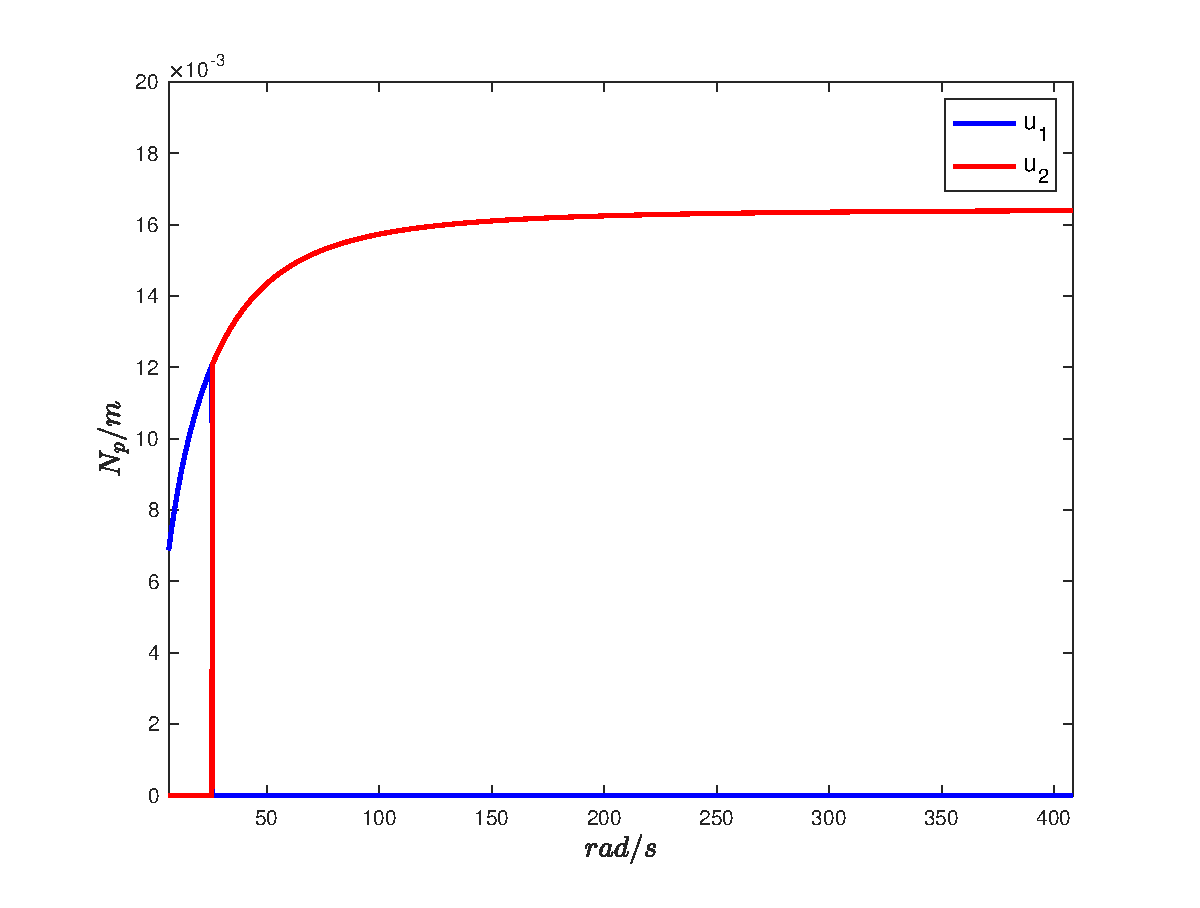
\includegraphics[scale=.425]{app_at_u}}\\
%\subfloat{\includegraphics[scale=.57]{phase_veloc_faraday_3}}
%\subfloat{\includegraphics[scale=.57]{attenuation_faraday_3}}\\
\subfloat{\includegraphics[scale=.425]{app_v_h}}
\subfloat{\includegraphics[scale=.425]{app_at_h}}
\caption{\textit{Velocidade de fase e atenua\c{c}\~ao de duas ondas el\'asticas e de uma onda eletromagn\'etica, que se propagam na dire\c{c}\~ao de $45^\circ$ no plano $xy$, e em fun\c{c}\~ao da frequ\^encia angular e de um campo magn\'etico externo. Caso Faraday.}}
\label{fig.disp_fa_45}
\end{figure}


\chapter{Modelo com Duas Fontes: S\'ismica e Eletromagn\'etica}
Normalmente, em levantamentos s\'ismicos s\~ao utilizadas somente fontes de ondas mec\^anicas, mas \'e poss\'ivel obtermos alguns resultados te\'oricos utilizando dois tipos de fontes simultaneamente. A seguir verificamos a inclus\~ao de uma fonte eletromagn\'etica junto com a fonte s\'ismica para o modelo de propaga\c{c}\~ao de ondas em meio 1D, homog\^eneo e com acoplamento total entre campos mec\^anicos e eletromagn\'eticos.

Incluindo uma fonte eletromagn\'etica $f(z,t)$ no sistema TAL, temos
\begin{align}
-\omega^2\rho\,u&=\frac{\partial}{\partial\,z}\left[(\lambda+2\,G)\frac{\partial\,u}{\partial\,z}-\mu h^0h\right]+F(z,\omega)\\\nonumber\\\
-i\,\omega\,h&=\frac{\partial}{\partial\,z}\left(V_H\frac{\partial\,h}{\partial\,z}-h^0\frac{\partial\,u}{\partial\,t}\right)-V_H f(z,t).
\end{align}
As solu\c{c}\~oes para esse novo sistema com duas fontes s\~ao dadas por 
\begin{align*}
u(k,\omega)&=u_1(k,\omega)+g_2(k,\omega)\,h_1(k,\omega)\\
h(k,\omega)&=g_1(k,\omega)\,u_1(k,\omega)+h_1(k,\omega),
\end{align*}
onde,
\begin{align*}
g_2(k,\omega)&=\frac{-i\,k\,\mu_0h^0}{(\lambda+2\,G)k^2-\omega^2\rho}\\\\
u_1(k,\omega)&=\frac{F}{(\lambda+2\,G)\,k^2-\omega^2\rho+i\,k\,\mu_0h^0g_1}\\\\
h_1(k,\omega)&=\frac{-V_Hf}{V_Hk^2-\omega^2\rho+k\,\omega\,h^0g_2}.
\end{align*}
Finalmente, se o acoplamento das ondas \'e parcial, temos
\begin{align*}
u_p(k,\omega)&=\frac{F}{(\lambda+2\,G)\,k^2-\omega^2\rho}\\
h_p(k,\omega)&=g_1(k,\omega)\,u_p(k,\omega)-\frac{V_Hf}{V_Hk^2-\omega^2\rho} .
\end{align*}
Observe que, para sistemas parcialmente acoplados, a solu\c{c}\~ao para ondas mec\^anicas permanece sem influ\^encia de for\c{c}as eletromagn\'eticas mesmo com a inclus\~ao de uma fonte eletromagn\'etica junto com a fonte s\'ismica. 

\begin{figure}
\centering
\includegraphics[scale=.73]{u_homo_Ff}
\caption{\textit{Considerando duas fontes, temos a amplitude de onda mec\^anica para sistema totalmente acoplado em cima e parcialmente acoplado embaixo.}}
\end{figure}

\begin{figure}
\centering
\includegraphics[scale=.73]{h_homo_Ff}
\caption{\textit{Considerando duas fontes, temos a amplitude da varia\c{c}\~ao magn\'etica para sistema totalmente acoplado em cima e parcialmente acoplado embaixo.}}
\end{figure}

TO CITE THE GRAPHICS in THE BODY TEXT\\
TO BUILD ANOTHER GRAPHICS CONSIDERING THE MAGNETIC VISCOSITY AT ELECTROMAGNETIC SOURCE.\\
THE ELECTROMAGNETIC SOURCE PRODUCE A LOT'S OF NOISES IN THE GRAPHICS (SPECIALLY IF WE INCLUDE VH) AND WE WILL PUSH THAT MODEL TO APPENDIX.





\end{document}